%%%%%%%%%%%%%%%%%%%%%%%%%%%%%%%%%%%%%%%%%%%%%%%%%%%%%%%%%%%%%%%%%%%%%%
%%  disstemplate.tex, to be compiled with latex.		     %
%%  08 April 2002	Version 4				     %
%%%%%%%%%%%%%%%%%%%%%%%%%%%%%%%%%%%%%%%%%%%%%%%%%%%%%%%%%%%%%%%%%%%%%%
%%								     %
%%  Writing a Doctoral Dissertation with LaTeX at		     %
%%	the University of Texas at Austin			     %
%%								     %
%%  (Modify this ``template'' for your own dissertation.)	     %
%%								     %
%%%%%%%%%%%%%%%%%%%%%%%%%%%%%%%%%%%%%%%%%%%%%%%%%%%%%%%%%%%%%%%%%%%%%%


\documentclass[12pt]{report}	% The documentclass must be ``report''.

\usepackage{utdiss2}  		% Dissertation package style file.


%%%%%%%%%%%%%%%%%%%%%%%%%%%%%%%%%%%%%%%%%%%%%%%%%%%%%%%%%%%%%%%%%%%%%%
% Optional packages used for this sample dissertation. If you don't  %
% need a capability in your dissertation, feel free to comment out   %
% the package usage command.					     %
%%%%%%%%%%%%%%%%%%%%%%%%%%%%%%%%%%%%%%%%%%%%%%%%%%%%%%%%%%%%%%%%%%%%%%

\usepackage{amsmath,amsthm,amsfonts,amscd} 
				% Some packages to write mathematics.
\usepackage{eucal} 	 	% Euler fonts
\usepackage{verbatim}      	% Allows quoting source with commands.
%\usepackage{makeidx}       	% Package to make an index.
\usepackage{psfig}         	% Allows inclusion of eps files.
\usepackage{epsfig}         	% Allows inclusion of eps files.
\usepackage{citesort}         	% 
\usepackage{url}		% Allows good typesetting of web URLs.
%\usepackage{draftcopy}		% Uncomment this line to have the
				% word, "DRAFT," as a background
				% "watermark" on all of the pages of
				% of your draft versions. When ready
				% to generate your final copy, re-comment
				% it out with a percent sign to remove
				% the word draft before you re-run
				% Makediss for the last time.
\usepackage{xspace}
\usepackage{parskip}
\usepackage{wrapfig}
\usepackage{times}
\usepackage{graphicx}
\usepackage{titling}
\usepackage{titlesec}
\usepackage{subfig}
\usepackage{bigstrut}
\usepackage{multirow}
\usepackage{booktabs}
\usepackage{array}
%\usepackage[T1]{fontenc}
%\usepackage[sc]{mathpazo} % Use the great palatino font provided by the mathpazo package. Add osf for old style figures
\usepackage{arial} % default for \textsf
\usepackage{inconsolata} % default for \texttt
\usepackage[usenames,dvipsnames]{xcolor}

\author{Yuhao Zhu}  	% Required

\address{1630 W 6th St.\\ Austin, Texas 78703}  % Required

\title{Energy-Efficient Mobile Web Computing}   % Required

%%%%%%%%%%%%%%%%%%%%%%%%%%%%%%%%%%%%%%%%%%%%%%%%%%%%%%%%%%%%%%%%%%%%%%
% NOTICE: The total number of supervisors and other members %%%%%%%%%%
%%%%%%%%%%%%%%% MUST be seven (7) or less! If you put in more, %%%%%%%
%%%%%%%%%%%%%%% they are put on the page after the Committee %%%%%%%%%
%%%%%%%%%%%%%%% Certification of Approved Version page. %%%%%%%%%%%%%%
%%%%%%%%%%%%%%%%%%%%%%%%%%%%%%%%%%%%%%%%%%%%%%%%%%%%%%%%%%%%%%%%%%%%%%

%%%%%%%%%%%%%%%%%%%%%%%%%%%%%%%%%%%%%%%%%%%%%%%%%%%%%%%%%%%%%%%%%%%%%%
%
% Enter names of the supervisor and co-supervisor(s), if any,
% of your dissertation committee. Put one name per line with
% the name in square brackets. The name on the last line, however,
% must be in curly braces.
%
% If you have only one supervisor, the entry below will read:
%
%	\supervisor
%		{Supervisor's Name}
%
% NOTE: Maximum three supervisors. Minimum one supervisor.
% NOTE: The Office of Graduate Studies will accept only two supervisors!
% 
%
\supervisor
	{Vijay Janapa Reddi}

%%%%%%%%%%%%%%%%%%%%%%%%%%%%%%%%%%%%%%%%%%%%%%%%%%%%%%%%%%%%%%%%%%%%%%
%
% Enter names of the other (non-supervisor) members(s) of your
% dissertation committee. Put one name per line with the name
% in square brackets. The name on the last line, however, must
% be in curly braces.
%
% NOTE: Maximum six other members. Minimum zero other members.
% NOTE: The Office of Graduate Studies may restrict you to a total
%	of six committee members.
%
%
\committeemembers
	[Lizy K. John]
	[Derek Chiou]
	[Christine Julien]
	{Scott Mahlke}

%%%%%%%%%%%%%%%%%%%%%%%%%%%%%%%%%%%%%%%%%%%%%%%%%%%%%%%%%%%%%%%%%%%%%%

\previousdegrees{B.S., M.S.}
     % The abbreviated form of your previous degree(s).
     % E.g., \previousdegrees{B.S., MBA}.
     %
     % The default value is `B.S., M.S.'

%\graduationmonth{...}      
     % Graduation month, either May, August, or December, in the form
     % as `\graduationmonth{May}'. Do not abbreviate.
     %
     % The default value (either May, August, or December) is guessed
     % according to the time of running LaTeX.

%\graduationyear{...}   
     % Graduation year, in the form as `\graduationyear{2001}'.
     % Use a 4 digit (not a 2 digit) number.
     %
     % The default value is guessed according to the time of 
     % running LaTeX.

%\typist{...}       
     % The name(s) of typist(s), put `the author' if you do it yourself.
     % E.g., `\typist{Maryann Hersey and the author}'.
     %
     % The default value is `the author'.


%%%%%%%%%%%%%%%%%%%%%%%%%%%%%%%%%%%%%%%%%%%%%%%%%%%%%%%%%%%%%%%%%%%%%%
% Commands for master's theses and reports.			     %
%%%%%%%%%%%%%%%%%%%%%%%%%%%%%%%%%%%%%%%%%%%%%%%%%%%%%%%%%%%%%%%%%%%%%%
%
% If the degree you're seeking is NOT Doctor of Philosophy, uncomment
% (remove the % in front of) the following two command lines (the ones
% that have the \ as their second character).
%
%\degree{MASTER OF ARTS}
%\degreeabbr{M.A.}

% Uncomment the line below that corresponds to the type of master's
% document you are writing.
%
%\masterreport
%\masterthesis


%%%%%%%%%%%%%%%%%%%%%%%%%%%%%%%%%%%%%%%%%%%%%%%%%%%%%%%%%%%%%%%%%%%%%%
% Some optional commands to change the document's defaults.	     %
%%%%%%%%%%%%%%%%%%%%%%%%%%%%%%%%%%%%%%%%%%%%%%%%%%%%%%%%%%%%%%%%%%%%%%
%
%\singlespacing
%\oneandonehalfspacing

%\singlespacequote
\oneandonehalfspacequote

\topmargin 0.125in	% Adjust this value if the PostScript file output
			% of your dissertation has incorrect top and 
			% bottom margins. Print a copy of at least one
			% full page of your dissertation (not the first
			% page of a chapter) and measure the top and
			% bottom margins with a ruler. You must have
			% a top margin of 1.5" and a bottom margin of
			% at least 1.25". The page numbers must be at
			% least 1.00" from the bottom of the page.
			% If the margins are not correct, adjust this
			% value accordingly and re-compile and print again.
			%
			% The default value is 0.125"

		% If you want to adjust other margins, they are in the
		% utdiss2-nn.sty file near the top. If you are using
		% the shell script Makediss on a Unix/Linux system, make
		% your changes in the utdiss2-nn.sty file instead of
		% utdiss2.sty because Makediss will overwrite any changes
		% made to utdiss2.sty.

%%%%%%%%%%%%%%%%%%%%%%%%%%%%%%%%%%%%%%%%%%%%%%%%%%%%%%%%%%%%%%%%%%%%%%
% Some optional commands to be tested.				     %
%%%%%%%%%%%%%%%%%%%%%%%%%%%%%%%%%%%%%%%%%%%%%%%%%%%%%%%%%%%%%%%%%%%%%%

% If there are 10 or more sections, 10 or more subsections for a section,
% etc., you need to make an adjustment to the Table of Contents with the
% command \longtocentry.
%
%\longtocentry 



%%%%%%%%%%%%%%%%%%%%%%%%%%%%%%%%%%%%%%%%%%%%%%%%%%%%%%%%%%%%%%%%%%%%%%
%	Some math support.					     %
%%%%%%%%%%%%%%%%%%%%%%%%%%%%%%%%%%%%%%%%%%%%%%%%%%%%%%%%%%%%%%%%%%%%%%
%
%	Theorem environments (these need the amsthm package)
%
%% \theoremstyle{plain} %% This is the default

\newtheorem{thm}{Theorem}[section]
\newtheorem{cor}[thm]{Corollary}
\newtheorem{lem}[thm]{Lemma}
\newtheorem{prop}[thm]{Proposition}
\newtheorem{ax}{Axiom}

\theoremstyle{definition}
\newtheorem{defn}{Definition}[section]

\theoremstyle{remark}
\newtheorem{rem}{Remark}[section]
\newtheorem*{notation}{Notation}

%\numberwithin{equation}{section}


%%%%%%%%%%%%%%%%%%%%%%%%%%%%%%%%%%%%%%%%%%%%%%%%%%%%%%%%%%%%%%%%%%%%%%
%	Macros.							     %
%%%%%%%%%%%%%%%%%%%%%%%%%%%%%%%%%%%%%%%%%%%%%%%%%%%%%%%%%%%%%%%%%%%%%%
%
%	Here some macros that are needed in this document:


\newcommand{\latexe}{{\LaTeX\kern.125em2%
                      \lower.5ex\hbox{$\varepsilon$}}}

\newcommand{\amslatex}{\AmS-\LaTeX{}}

\chardef\bslash=`\\	% \bslash makes a backslash (in tt fonts)
			%	p. 424, TeXbook

\newcommand{\cn}[1]{\texttt{\bslash #1}}

\makeatletter		% Starts section where @ is considered a letter
			% and thus may be used in commands.
\def\square{\RIfM@\bgroup\else$\bgroup\aftergroup$\fi
  \vcenter{\hrule\hbox{\vrule\@height.6em\kern.6em\vrule}%
                                              \hrule}\egroup}
\makeatother		% Ends sections where @ is considered a letter.
			% Now @ cannot be used in commands.

%\makeindex    % Make the index

%%%%%%%%%%%%%%%%%%%%%%%%%%%%%%%%%%%%%%%%%%%%%%%%%%%%%%%%%%%%%%%%%%%%%%
%		The document starts here.			     %
%%%%%%%%%%%%%%%%%%%%%%%%%%%%%%%%%%%%%%%%%%%%%%%%%%%%%%%%%%%%%%%%%%%%%%

\begin{document}

\copyrightpage          % Produces the copyright page.


%
% NOTE: In a doctoral dissertation, the Committee Certification page
%		(with signatures) is BEFORE the Title page.
%	In a masters thesis or report, the Signature page
%		(with signatures) is AFTER the Title page.
%
%	If you are writing a masters thesis or report, you MUST REVERSE
%	the order of the \commcertpage and \titlepage commands below.
%
\commcertpage           % Produces the Committee Certification
			%   of Approved Version page (doctoral)
			%   or Signature page (masters).
			%		20 Mar 2002	cwm

\titlepage              % Produces the title page.


\graphicspath{{figs/}}
\newcommand{\website}[1]{{\tt #1}}
\newcommand{\program}[1]{{\tt #1}}
\newcommand{\benchmark}[1]{{\it #1}}
\newcommand{\fixme}[1]{{\textcolor{red}{$fixme:$~\textit{#1}}}}

\renewcommand{\figurename}{Fig.}
\renewcommand{\paragraph}[1]{\textbf{#1}~~}
\newcommand{\figline}{{\vspace*{.05in}\hline}}

\newcommand{\Sect}[1]{Section.~\ref{#1}}
\newcommand{\Fig}[1]{Figure.~\ref{#1}}
\newcommand{\Tbl}[1]{Table~\ref{#1}}
\newcommand{\Equ}[1]{Equation.~\ref{#1}}
\newcommand{\Apx}[1]{Appendix.~\ref{#1}}

\newcommand{\specialcell}[2][c]{\begin{tabular}[#1]{@{}l@{}}#2\end{tabular}}
\newcommand{\note}[1]{\textcolor{red}{#1}}

\newcolumntype{x}[1]{>{\centering\arraybackslash\hspace{0pt}}p{#1}}
\newcolumntype{y}[1]{>{\raggeright\arraybackslash\hspace{0pt}}p{#1}}

\newcommand{\greenweb}{{\fontfamily{cmtt}\selectfont GreenWeb}\xspace}
\newcommand{\webcore}{{\fontfamily{cmtt}\selectfont WebCore}\xspace}
\newcommand{\webrt}{{\fontfamily{cmtt}\selectfont WebRT}\xspace}
\newcommand{\autogreen}{\textsc{AutoGreen}\xspace}
\newcommand{\ebs}{\textsc{EBS}\xspace}

\newcommand{\RNum}[1]{\uppercase\expandafter{\romannumeral #1\relax}}


\begin{dedication}
%\index{Dedication@\emph{Dedication}}%
Dedicated to my wife Shirley.
\end{dedication}


%!TEX root=../paper.tex

\begin{acknowledgments}		% Optional
%\index{Acknowledgments@\emph{Acknowledgments}}%
I wish to thank the multitudes of people who helped me throughout this journey. First and foremost, I would like to thank The University of Texas at Austin, and the taxpayers of the great state of Texas, for supporting me to pursue a degree in a filed that I am truly passionate about. Among many things, UT Austin provides a stimulating, diverse, and welcoming environment for intellectual explorations that one could ever imagine having.

I would like to express my sincere gratitude to my advisor Vijay Janapa Reddi, who turned me from a student to a researcher. I came to UT as an avocational computer architecture enthusiast. Vijay patiently taught me how to turn half-baked ideas to high-quality research papers, and how to turn individual papers into a dissertation. I appreciate the many technical and visionary discussions that he had with me while walking on campus.

Vijay also trained me to be a long-term investor. In my first semester working with Vijay, he spent over a thousand dollars to send us to a half-day course on information visualization. He later sent us to other venues such as training mental agility. Although some of these investments might have not paid off immediately toward a paper---some never will---it gradually shaped my mindset beyond just becoming a better graduate student to becoming a better person, which I will forever benefit from.

I would also like to thank other members of my dissertation committee: Lizy John, Derek Chiou, Christine Julien, and Scott Mahlke. Their keen insights and feedbacks are absolutely invaluable in developing and refining the concepts in my dissertation. In addition, Lizy taught me Computer Performance Evaluation and Benchmarking, and Derek taught me Parallel Architecture; both helped me form the computer architecture foundations. Special thanks to Christine and Scott who gave me many pieces of advice and wrote me recommendation letters for my job search.

During my time at UT, I also had the privilege to interact and work with other faculty members, in particular Mattan Erez, Mohit Tiwari, and Yale Patt. Mattan is a calm, sharp, and encouraging human being who I look up to. He taught me Computer Architecture during my first semester in UT (and this country), which is the reason that I now can talk comfortably about computer architecture. Mohit is always there to provide me lots of advice in career development. I worked with Dr. Patt during my first year as a graduate researcher and as a teaching assistant for his Computer Architecture course in my second semester. The interactions with him provided me unique perspectives that I would have gotten from nowhere otherwise.

I had four summer internships during my graduate study, and I want to thank my mentors during each internship. Osvaldo Colavin was my mentor at STMicroelectronics in summer 2011. We first met at DAC that year at San Diego, and he later made me an internship offer. I thank Osvaldo for truly opening my eyes to the industry for the first time. Mauricio Breternitz was my mentor during my two internships at AMD Research in summer 2012 and 2013. I admire his incredible experience in hardware and software industry. He gave me the opportunity to integrate several AMD specific hardware performance counters into the \texttt{libpfm} in my first internship, and gave me lots of freedom to explore Web browser caching during my second internship. Nat Duca was my mentor during my internship at the Google Chrome team in summer 2015. Even to this day I couldn't believe that I had worked with Nat. Nat is an incredible person and great friend who continues to help me after the internship. He also connected me with many other wonderful Chrome engineers---the reason that the Web is well alive and kicking!

My lab mates and friends at UT Austin not only help me academically, but also always encourage me to never back off from challenges, and I greatly thank them for that. Jingwen Leng and Aditya Srikanth helped me with my first project to get my research started. Jingwen and I had a lot of fun beyond research. Among many things, we often drove to Houston just to play snooker, and flew to UK to watch snooker games. Daniel Richins and Wenzhi Cui helped me with the Node.js project. Wenzhi would always listen to my nonsense ideas. Matthew Halpern helped me with \textit{everything} since he joined. He acts as a cheerleader when I am down and keeps me sane. I have also met many friends at UT and Austin who I want to thank: Song Zhang, Haishan Zhu, Tianhao Zheng, Yazhou Zu, Yong Li, Minsoo Rhu, Milad Hashemi, Faruk Guvenilir, and Khubaib. Special thanks to Khubaib who mentored me during my first year working with Dr. Patt and continued to support me after that.

I am grateful to the Google Ph.D. fellowship for supporting my Ph.D. research. Matt Welsh is my fellowship mentor, who is a true enemy of hogwash. Matt has supported my research throughout my entire graduate study by being an advocator inside Google for our research. He also generously wrote a recommendation letter for my job search. I was also supported by the Microelectronics and Computer Development Fellowship at the Cockrell School of Engineering in UT Austin during my second year.

I also want to thank my undergraduate advisor Yangdong (Steve) Deng at Tsinghua University. I was an undergrad at Beihang University, and Steve just came back from the United States to start his lab. I anxiously sent him a cold email expressing my interests, and (not) surprisingly he decided to bring me to the lab. We together worked on GPGPU programming and microarchitecture, which greatly raised my interests in system architectures. He encourages me to think big and makes me believe that I, too, could publish first-class research results. I would never get a Ph.D. if not for the one year working and interacting with Steve.

Most importantly, not a single word of this dissertation would happen without the support of my loving family. My parents, Qinxiong Zhu and Xiaojing Yu, care about me more than themselves and never hold me off in pursuing whatever I am passionate about, even if that means they only saw me four times in the past seven years. Finally, I thank my wife Yunjing Luo for always being there since we first met in 2012. Although she believes that I could have finished Ph.D. sooner without her, I believe otherwise.

\end{acknowledgments}

%!TEX root=paper.tex

% The abstract is required. Note the use of ``utabstract'' instead of
% ``abstract''! This was necessary to fix a page numbering problem.
% The abstract heading is generated automatically.
% Do NOT use \begin{abstract} ... \end{abstract}.
%
\utabstract
\indent
Next-generation Web services will be primarily accessed through mobile devices. However, mobile devices are low-performance and stringently energy-constrained. In this thesis, I propose the design of a high-performance and energy-efficient mobile computing substrate. It is a hardware/software co-designed system that delivers satisfactory user quality-of-service (QoS) experience on a mobile energy budget. The key insight that the traditional interfaces between different Web stacks need to be enhanced with new abstractions that express user QoS experience and that expose architectural-level complexities. On the basis of the enhanced interfaces, I propose synergistic cross-layer optimizations across the processor architecture, Web runtime, programming language, and application layers to maximize the whole system efficiency. The proposal is likely to have a long-term impact because the target application domain, the Web, is becoming a universal mobile development platform, and our solutions target the fundamental computation layers of the Web domain.



\tableofcontents   % Table of Contents will be automatically
                   % generated and placed here.

\listoftables      % List of Tables and List of Figures will be placed
\listoffigures     % here, if applicable.


%%%%%%%%%%%%%%%%%%%%%%%%%%%%%%%%%%%%%%%%%%%%%%%%%%%%%%%%%%%%%%%%%%%%%%
% Actual text starts here.					     %
%%%%%%%%%%%%%%%%%%%%%%%%%%%%%%%%%%%%%%%%%%%%%%%%%%%%%%%%%%%%%%%%%%%%%%
%
% Including external files for each chapter makes this document simpler,
% makes each chapter simpler, and allows for generating test documents
% with as few as zero chapters (by commenting out the include statements).
% This allows quicker processing by the Makediss command file in case you
% are not working on a specific, long and slow to compile chapter. You
% can even change the chapter order by merely interchanging the order
% of the include statements (something I found helpful in my own
% dissertation).
%
%!TEX root=../paper.tex

\chapter{Introduction}
\label{sec:intro}

Web technologies have shaped how we think, communicate, and innovate. Over the past decade, the Web's role shifted from solely information retrieval (Web 1.0) to providing interactive user experiences (Web 2.0). Now the Web is once again on the cusp of a new evolution that features automatic recognition, mining, and synthesis of user-originated ``big data.'' The driving force behind this evolution is today's most pervasive personal computing platform---mobile devices. It is estimated that 3~billion Web-connected mobile devices currently exist, and will reach nearly 50~billion by 2020~\cite{Evans:2011ys}. The trend is clear: next-generation Web services will be primarily accessed through mobile devices instead of desktops and laptops as in previous generations~\cite{KPCB-Internet-Trends15}.

While there are significant growth opportunities for mobile Web computing, standing in the way are technology challenges. Specifically, there is a fundamental tension between the ever-increasing computation intensity of Web technologies and the performance and energy-constraint nature of mobile devices. Such a mismatch between computational ``demand and supply'' leads to poor quality-of-service (QoS) experience, resulting in severe consequences. For example, Google estimated that ``a 400~ms delay leads to a 0.44\% drop in search volume.''~\cite{web:google} Similarly, Amazon concluded that a 1-second delay in webpage load time could translate to \$1.6 billion lost in sales annually~\cite{Eaton:2013uq}.

Conventional techniques to improve mobile compute capability have largely been focused on CPU design, especially by simply adopting desktop-oriented design techniques---to apply aggressive (micro-)architecture mechanisms for both single-core and multi-core performance improvement while relying the underlying circuit techniques (i.e., Dennard Scaling~\cite{dennard}) for power and energy-efficiency improvement~\cite{mobilecpu}. However, as the demise of graceful Dennard scaling becomes a reality, excessive power and energy consumption will eventually put such a CPU-centric, desktop-like design strategy to its end.

\paragraph{Thesis Statement} To provide sustainable mobile performance improvement while being energy-efficient, we must deviate away from the traditional CPU-only mentality. Instead, we must expand the research scope to the entire Web computing stack where performance and energy-efficiency can be maximized through exploiting synergistic cross-layer optimizations. My dissertation designs a hardware/software computing substrate that optimizes mobile Web performance and energy-efficiency across the application, programming language, Web runtime, and processor architecture layers.

\Sect{sec:intro:scope} first outlines my research scope with respect to the broad context of mobile computing. \Sect{sec:intro:work} then provides an overview of my research contributions and \Sect{sec:intro:impact} discusses the long-term impact of my dissertation work. \Sect{sec:intro:outline} outlines the rest of the dissertation and \Sect{sec:intro:prev} lists previously published materials that this dissertation draws upon.

\section{Research Scope}
\label{sec:intro:scope}

The rich scope of mobile Web computing involves two critical components: compute and network. The compute component can be further classified by approaches that are either client-centric or based on cloud-offloading. My research judiciously focuses on the client-side compute. In other words, it takes a compute-driven and client-centric approach. This section discusses my rational. The goal here is not to dismiss research in network and cloud computing community, but to explain the trade-offs and thereby set the context.

\paragraph{Compute-versus-Network} Traditionally when the scope of Web computing was merely about serving static webpages, Web performance was predominantly bottlenecked by network capability because very little processing was involved. However, this trend is changing. Over the past decade cellular network technology has improved dramatically. For example, the round-trip time is improved by two orders of magnitude from 2G to LTE ~\cite{4gtest}. Meanwhile, the computational requirements posed by new Web technologies (e.g., CSS3, HTML5, WebGL) keep increasing. For instance, under the same network condition the processing time for loading the same website from different years over the past decade has increased by as much as 10X~\cite{big-little}. The combined effect of faster network performance and higher computation demand implies that future mobile Web performance will be unattainable without improving the compute capability. I provide an in-depth computer-versus-network bottleneck analysis in \Sect{sec:motivation:perf}.

\paragraph{Client-versus-Cloud} Compute in mobile Web has been primarily carried out by client-side devices only. Recently researcher have started investigating a new compute paradigm where part of the computation is offloaded to cloud platforms through wireless connections---the so called mobile cloud computing (MCC). Although MCC is a promising approach that extends the capability of mobile devices for computation-intensive applications, it has three major limitations. First, today's Web applications are extremely dynamic where both data and code can be generated at runtime depending on user-specific information (e.g., via sensors). The dynamic nature of Web applications leads to frequent synchronizations between client and cloud that potentially undermine the performance and energy-efficiency benefits that MCC brings. Second, MCC assumes the availability of wireless connections, which limits its usage scenario. Third, MCC raises security and privacy concerns as data and computation are transmitted over the network.

The limitations stated above indicate that a handful questions need to be addressed for MCC to succeed. That said, future mobile Web computing systems will most certainly incorporate certain aspects of cloud-offloading, a quantitative trade-off study of which is warranted but beyond my scope.

\section{Research Contributions}
\label{sec:intro:work}

The key theme of my work is to deviate away from the general-purpose CPU-centric mindset and to take a holistic view of the mobile Web computation stack spanning application, Web browser runtime, and processor architecture layers. I contend that improving energy-efficiency and performance of mobile Web computing requires us to enhance the traditional computing interfaces with \textit{new abstractions} and to leverage the new interfaces for \textit{cross-layer optimizations}. As such, the central challenge of my research is to carefully forge new abstractions that expose optimization opportunities while enabling effective and practical optimization mechanisms.

At the application/Web browser boundary, current Web applications merely specify visual appearance and functionalities to the browser through Web languages such as HTML, CSS, and JavaScript. User QoS requirements (e.g., latency tolerance) are unexpressed. However, different users QoS requirements lead to different optimal runtime decisions for trading off QoS with energy consumption. Exposing user QoS expectations at the application level would allow the Web runtime to budget wisely the energy usage while delivering satisfactory user QoS experience.

At the Web browser/architecture boundary, the traditional interface provides to the Web browser runtime a simplistic and monolithic execution model of the hardware. However, today's mobile processors are becoming extremely complex, combining general-purpose cores that have different performance and energy characteristics~\cite{single-ISA} with special-purpose domain-specific accelerators. While the hardware upheaval promises performance and energy improvements for the mobile Web, its practical impact depends on how effective the Web browser can leverage it. I see both needs on specializing the processor architecture for the Web domain that enriches the runtime/architecture interface and on designing an intelligent Web browser runtime that can effectively manage the complex interface to optimize for energy-efficiency.

In the spirit of enhancing the traditional Web computing stack interfaces and leveraging the new interfaces to optimize each layer, my dissertation makes the following three contributions. \Fig{fig:framework} provides an overview of the contributions. Enhancements to the existing Web stack are shaded.

\begin{sidewaysfigure}
    \centering
    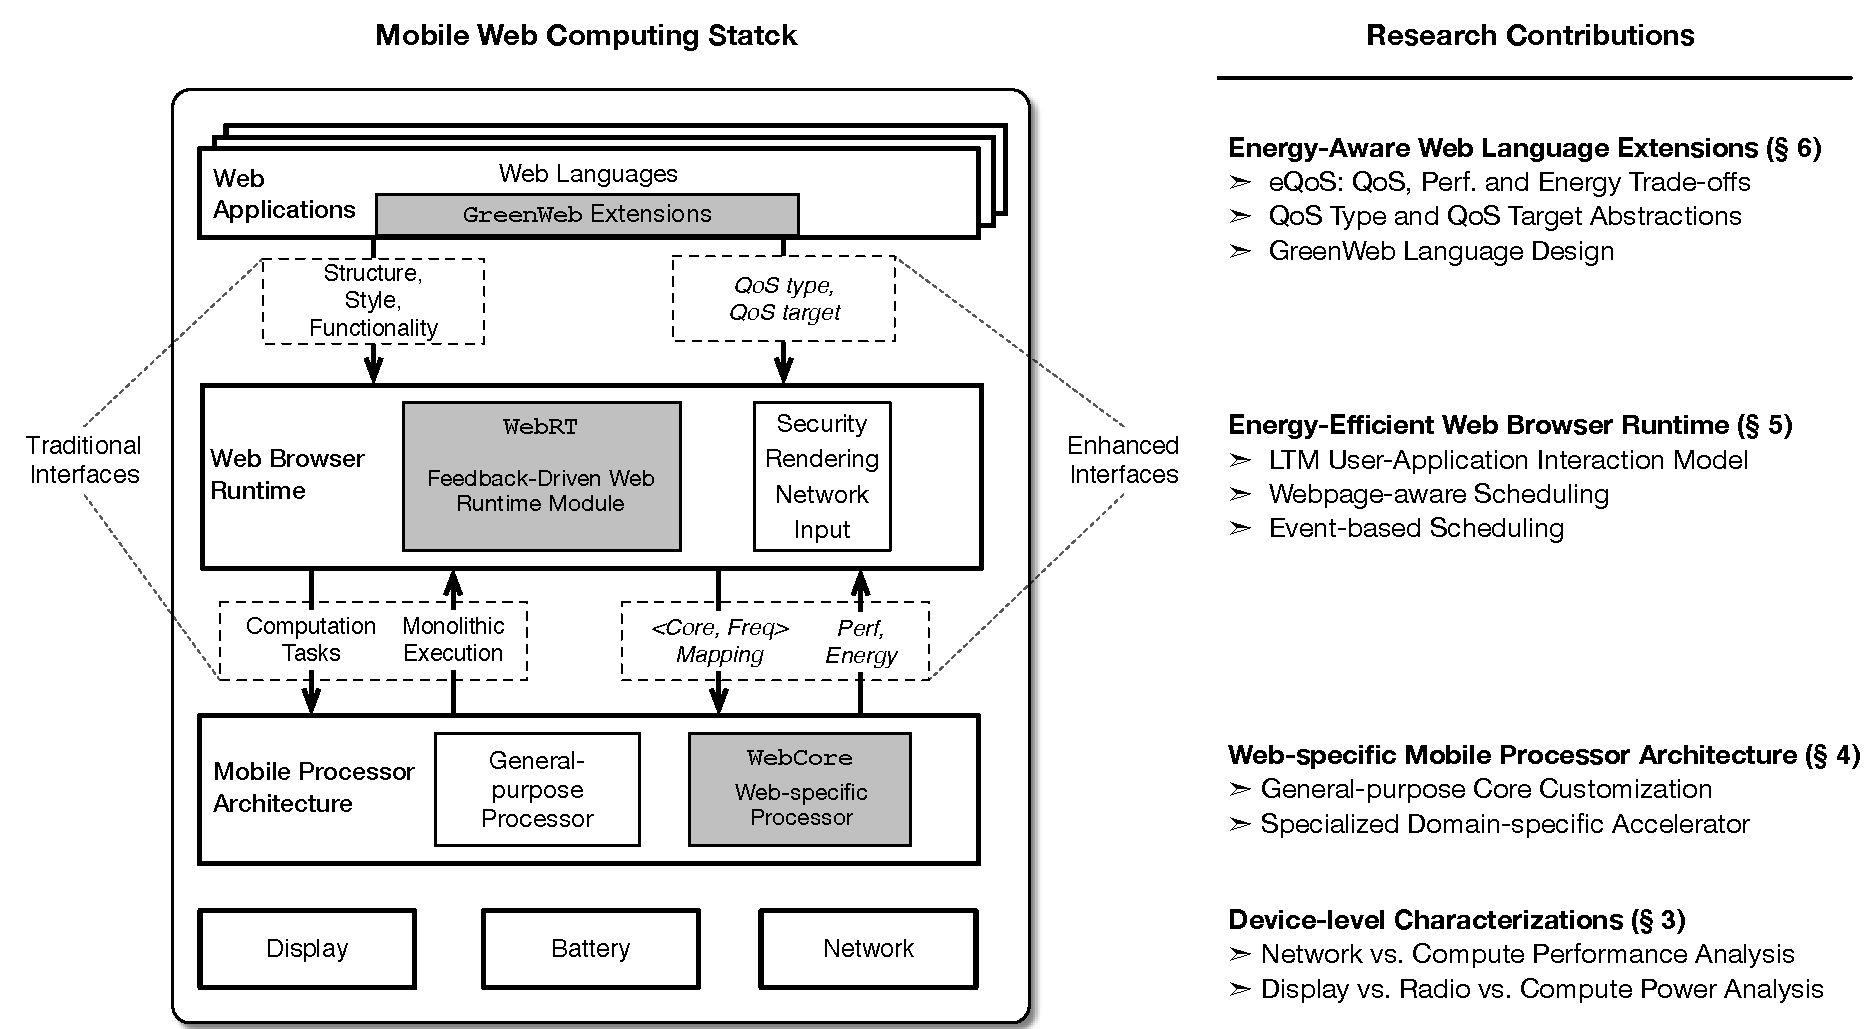
\includegraphics[trim=0 0 0 0, clip, width=1\columnwidth]{framework}
    \caption{Overview of my cross-layer research contributions.}
    \label{fig:framework}
\end{sidewaysfigure}

\begin{itemize}
\item \textbf{Web Language Extensions:} I propose \greenweb, a set of programming language extensions that let Web developers express user QoS expectations as program annotations. \greenweb enhances the traditional application-runtime interface with two new programming abstractions, QoS type and QoS target, that capture two critical aspects of user QoS experience. Exposing QoS requirements in Web applications effectively guides the underlying Web runtime to determine how to deliver the target QoS experience while minimizing the energy consumption. \greenweb does not pose any constraints on specific runtime implementations but instead supports general energy optimization techniques.

\item \textbf{Smart Web Browser Runtime:} I propose \webrt, a  mobile Web browser runtime that optimizes for energy-efficiency while delivering the specified user QoS requirements. Although \webrt is a generic runtime design, I demonstrate a prototype implementation based on the asymmetric chip-multiprocessor (ACMP) hardware architecture. ACMP exposes two new architecture-level abstractions: core type and core frequency. \webrt leverages the new abstractions and dynamically provisions the hardware resources according to user QoS requirements for energy savings. In addition, \webrt also continuously monitors the runtime execution behaviors to enable feedback-driven optimizations, which is critical considering the interactive nature of mobile applications.

\item \textbf{Web-Specific Processor Architecture:} I propose \webcore, a forward-looking mobile CPU architecture customized and specialized for the Web stack. The \webcore improves performance and energy-efficiency simultaneously by integrating domain-specific hardware that exploits critical computation kernels and data communication patterns. A key design goal of \webcore is maintain general-purpose programmability, which is vital to ensure its applicability to the complex Web software stack. Overall, \webcore deepens the heterogeneity of the mobile processor architecture and enlarges the performance-energy trade-off space that the Web runtime can take advantage of.
\end{itemize}

\section{Long-term Impact}
\label{sec:intro:impact}

Mobile hardware and Web software ecosystems undergo rapid design cycles to keep up with constant innovations. It is vital to ensure that any research contributions to this domain have long-term impact, or they perish.

The long-term impact of my work lies in two fundamental aspects. First, the problem that I study is a long-term research agenda. The key research challenge that my research focuses on, i.e., to improve performance and energy-efficiency, will always be at the forefront of mobile computing research. As the battleground of mobile computing gradually shifts into even smaller form factors such as wearables and Internet-of-Things (IoT) devices, improving performance and energy-efficiency of mobile computing is ever important.

Second, my proposed techniques are likely to have long-term applicability because they focus on the fundamental computation layers of Web technologies rather than tied to specifics of a particular platform. For instance, \webcore proposes a hardware units that optimizes CSS processing. Although new Web standards and specifications come and go, CSS processing as a cornerstone technology remains largely unchanged and thus can continue to benefit from \webcore. Similarly, the designs of \webrt and \greenweb are also generally applicable because they are do not rely on a particular form of underlying processor (micro-)architecture or application features.

\section{Dissertation Organization}
\label{sec:intro:outline}

The rest of my dissertation is organized as follows. \Sect{sec:background} introduces the preliminary knowledge of Web computing. \Sect{sec:motivation} quantitatively demonstrates the need for high-performance and energy-efficient computation in the mobile Web, which directly motivates the research theme of my work. \Sect{sec:arch}, \Sect{sec:runtime}, and \Sect{sec:lang} describe the proposed \webcore, \webrt, and \greenweb at the architecture, runtime, and programming language layer, respectively. \Sect{sec:conc} provides a retrospective and prospective view of my dissertation work. The retrospective part summarizes the principles distilled from this work on building a high-performance while energy-efficient mobile Web computing system; the prospective part suggests next steps for generalizing the principles and outlines potential research items for future work.

\section{Previously Published Material}
\label{sec:intro:prev}

This dissertation contains materials that are previously published in peer-reviewed conferences and journals:

\textbf{\Sect{sec:motivation}}. The network-versus-computer analysis in \Sect{sec:motivation:perf} contains results from the following paper: \textit{The Role of the CPU in Energy-Efficient Mobile Web Browsing}. Yuhao Zhu, Matthew Halpern and Vijay Janapa Reddi. In IEEE Micro, Jan/Feb 2015, 35(1):26-33 \cite{zhu2015role}. The power and energy characterizations in \Sect{sec:motivation:energy} contains results from the following paper: \textit{Mobile CPU's Rise to Power: Quantifying the Impact of Generational Mobile CPU Design Trends on Performance, Energy, and User Satisfaction}. Matthew Halpern, Yuhao Zhu and Vijay Janapa Reddi. In High Performance Computer Architecture (HPCA), 2016 \cite{mobilecpu}.

\textbf{\Sect{sec:arch}}. The design and implementation of \webcore are based on the following paper: \textit{WebCore: Architectural Support for Mobile Web Browsing}. Yuhao Zhu and Vijay Janapa Reddi. In International Symposium on Computer Architecture (ISCA), 2014 \cite{webcore}. \Sect{sec:arch} also contains results from the following journal paper that is currently under review: \textit{Optimizing General-Purpose CPUs for Energy-Efficient Mobile Web Computing}. Yuhao Zhu and Vijay Janapa Reddi. 2016 \cite{webcore-tocs}.

\textbf{\Sect{sec:runtime}}. The fundamental idea of \webrt is based on the following position paper:  \textit{Exploiting Webpage Characteristics for Energy-Efficient Mobile Web Browsing}. Yuhao Zhu, Aditya Srikanth, Jingwen Leng and Vijay Janapa Reddi. In Computer Architecture Letters (CAL), Oct 2012, 13(1):33-36 \cite{zhu2014exploiting}. The webpage-aware scheduler described in \Sect{sec:runtime:load} draws upon \textit{High-Performance and Energy-Efficient Mobile Web Browsing on Big/Little Systems}. Yuhao Zhu and Vijay Janapa Reddi.  In High Performance Computer Architecture (HPCA), 2013 \cite{big-little}. The event-based scheduler in \Sect{sec:runtime:ebs} draws upon \textit{Event-based Scheduling for Energy-Efficient QoS (eQoS) in Mobile Web Applications}. Yuhao Zhu, Matthew Halpern and Vijay Janapa Reddi. In High Performance Computer Architecture (HPCA), 2015 \cite{ebs}.

\textbf{\Sect{sec:lang}}. The \greenweb language extensions and the \autogreen annotation framework are based on the following paper: \textit{GreenWeb: Language Extensions for QoS-aware Energy-Efficient Mobile Web Computing}. Yuhao Zhu and Vijay Janapa Reddi. In Programming Language Design and Implementation (PLDI), 2016 \cite{greenweb}.



%!TEX root=paper.tex

\chapter{The Need for High-Performance and Energy-Efficient Computation in Mobile Web}
\label{sec:motivation}

This section quantitatively demonstrates the importance of \textit{computation}, among other components such as network and display, to mobile Web's performance and energy consumption. The observations discussed in this section directly motivate my research to focus on the computation layer of the mobile Web and to improve its performance and energy-efficiency.

The computation layer involves many mobile SoC components, such as CPU, GPU, and domain-specific accelerators. My proposal specifically focuses on the CPU for the following two reasons. First, CPU is the most heavily exercised computation component for Web applications because the Web runtime primarily targets CPUs. GPUs' usage, although providing critical performance benefits, is still limited to specific tasks such as rasterization and compositing~\cite{gpucompositor}. The key computations such as layout and JavaScript execution are still solely performed on general-purpose CPUs. Second, CPU serves as an incubator for future accelerators---we must first understand computation kernels' characteristics on CPUs before they can be accelerated.
%In fact, one of my proposed techniques is the accelerator design for a key Web computation kernel based on its CPU execution behaviors.
%From now on, I use computation and CPU interchangeably unless otherwise noted.

In the rest of this section, I first show that mobile Web performance increasingly depends on the computational capability of mobile CPUs, indicating the need for a high-performance computation~(\Sect{sec:motivation:perf}). I then show that mobile devices' power consumption is increasingly dominated by CPUs, calling for an energy-efficient computation~(\Sect{sec:motivation:energy}). Note that all the results presented in \Sect{sec:motivation:energy} are adapted from a recent research project~\cite{mobilecpu} that I collaborated on and contributed to.

\section{The Importance of High-Performance Computation in Mobile Web}
\label{sec:motivation:perf}

Computation and network largely dictate the performance of mobile Web. Conventional wisdom suggests that mobile Web performance is primarily limited by the network latency. In this section, I quantify the impact of CPU and network performance by experimentally comparing how the webpage load time varies with different CPU and network performance on today's high-end smartphone Galaxy S5. I show that as cellular network technologies evolve over generations, mobile Web performance becomes sensitive to CPU performance.

%Network performance is typically evaluated in two metrics: latency and bandwidth. Prior work has shown that in the mobile context, network latency---typically evaluated by round-trip time (RTT)---has a much more significant impact than network bandwidth~\cite{HPBN, browser-slow}. Therefore, we focus only on the latency aspect of network performance.

\paragraph{Network Impact} To study the impact of network latency of various cellular network generations, we host all the webpages on a Web server, into which we manually inject delay. We then use Wi-Fi on the smartphone to access the webpages. Since Wi-Fi has significantly lower latency than the current 4G/LTE network, the delay injection lets us mimic a wide range of network latencies. 
%This methodology is a well-established technique to control cellular network latency~\cite{browser-slow}.

Holding the CPU performance at its peak, \Fig{fig:network_bottleneck} shows the webpage load time with respect to different network latencies. We superimpose the figure with different mobile network technologies' typical latencies derived from both technical specifications as well as real measurements in the field~\cite{HPBN, carrier_measure}. We observe that reducing the network latency from an adverse 3G connection at 2,000~ms to an LTE connection at 100~ms results in a 9.5X speedup in webpage load time from 38~seconds to 4~seconds. As the network latency further improves within the range of LTE network latency (50$\sim$100~ms), the network latency has only a marginal impact on the overall webpage load time. This is because at this point the fast network accesses are hidden behind CPU computations in the asynchronous execution model; the application is largely CPU-bound. Further reducing the network latency from LTE to Wi-Fi has almost no effect.

\paragraph{Computation Impact} As the network latency becomes low (e.g., under the LTE technology), the CPU performance starts playing a significant role in the mobile Web performance. To study how the CPU performance affects the webpage load time, we mimic a wide range of CPU performance capabilities by leveraging S5's 14 frequency settings. Note that we use frequency only as a \textit{proxy} for CPU performance, it is \emph{not} our intention to study the impact of a particular CPU's frequency itself.~\Fig{fig:cpu_bottleneck} shows how webpage load time changes with CPU performance under a 100~ms RTT (LTE-like cellular network connectivity). As the CPU frequency decreases from the highest to the lowest by about 6X (2.5 GHz to 0.4 GHz), the webpage load time slows down by as much as 4.5X from 4~seconds to about 18~seconds, indicating strong sensitivity to CPU performance.

\begin{figure}[t]
\centering
  \begin{minipage}[b]{0.47\columnwidth}
    \centering
    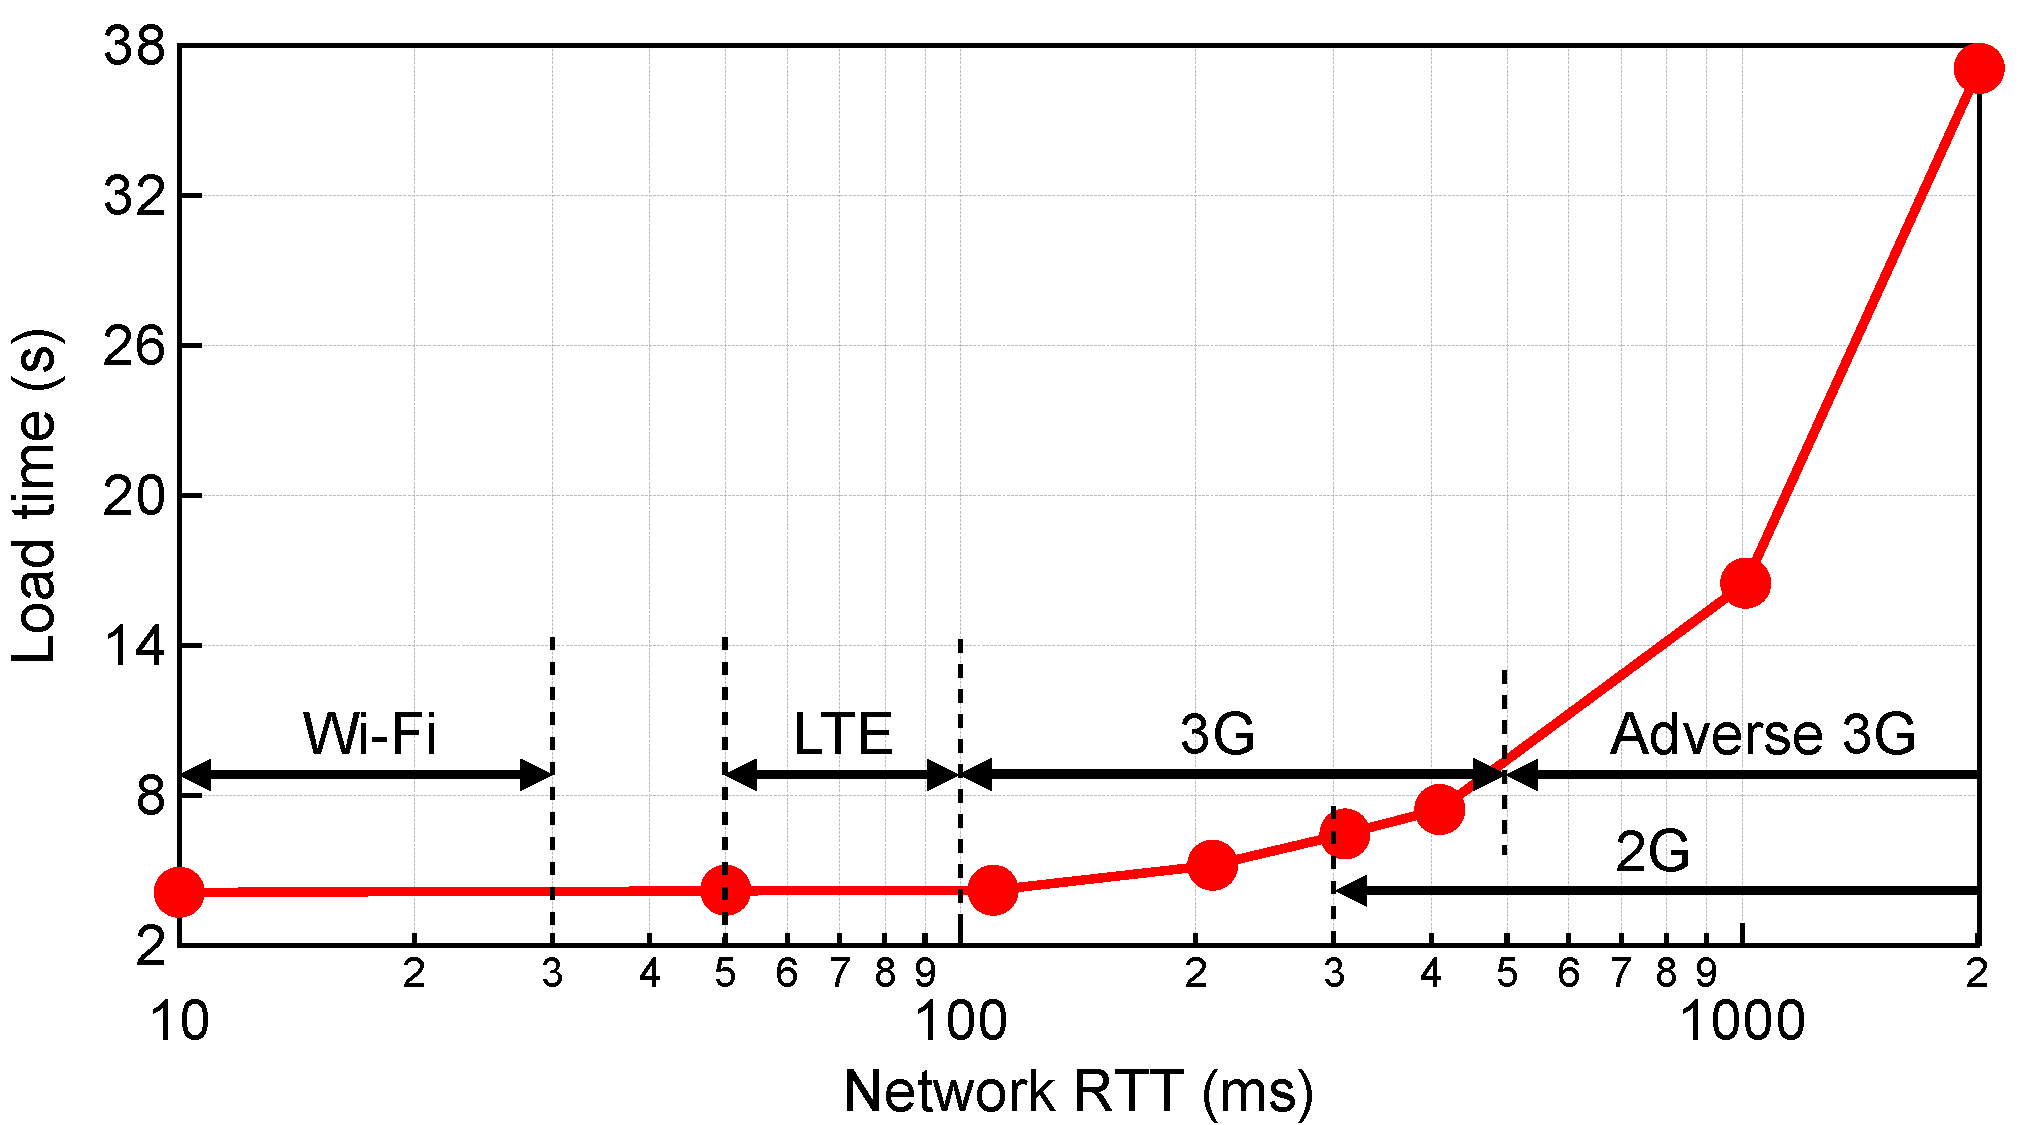
\includegraphics[trim=0 0 0 0, clip, width=\columnwidth]{network_bottleneck}
    \caption{Webpage load time with respect to changing network latency. Each
marker corresponds to an RTT value. We also superimpose the round-trip time
(RTT) range for different cellular technologies derived from both technical
specifications as well as real measurements in the field~\cite{HPBN,
carrier_measure}.}
  \label{fig:network_bottleneck}
  \end{minipage}
  \hspace*{15pt}
  \begin{minipage}[b]{0.47\columnwidth}
    \centering
    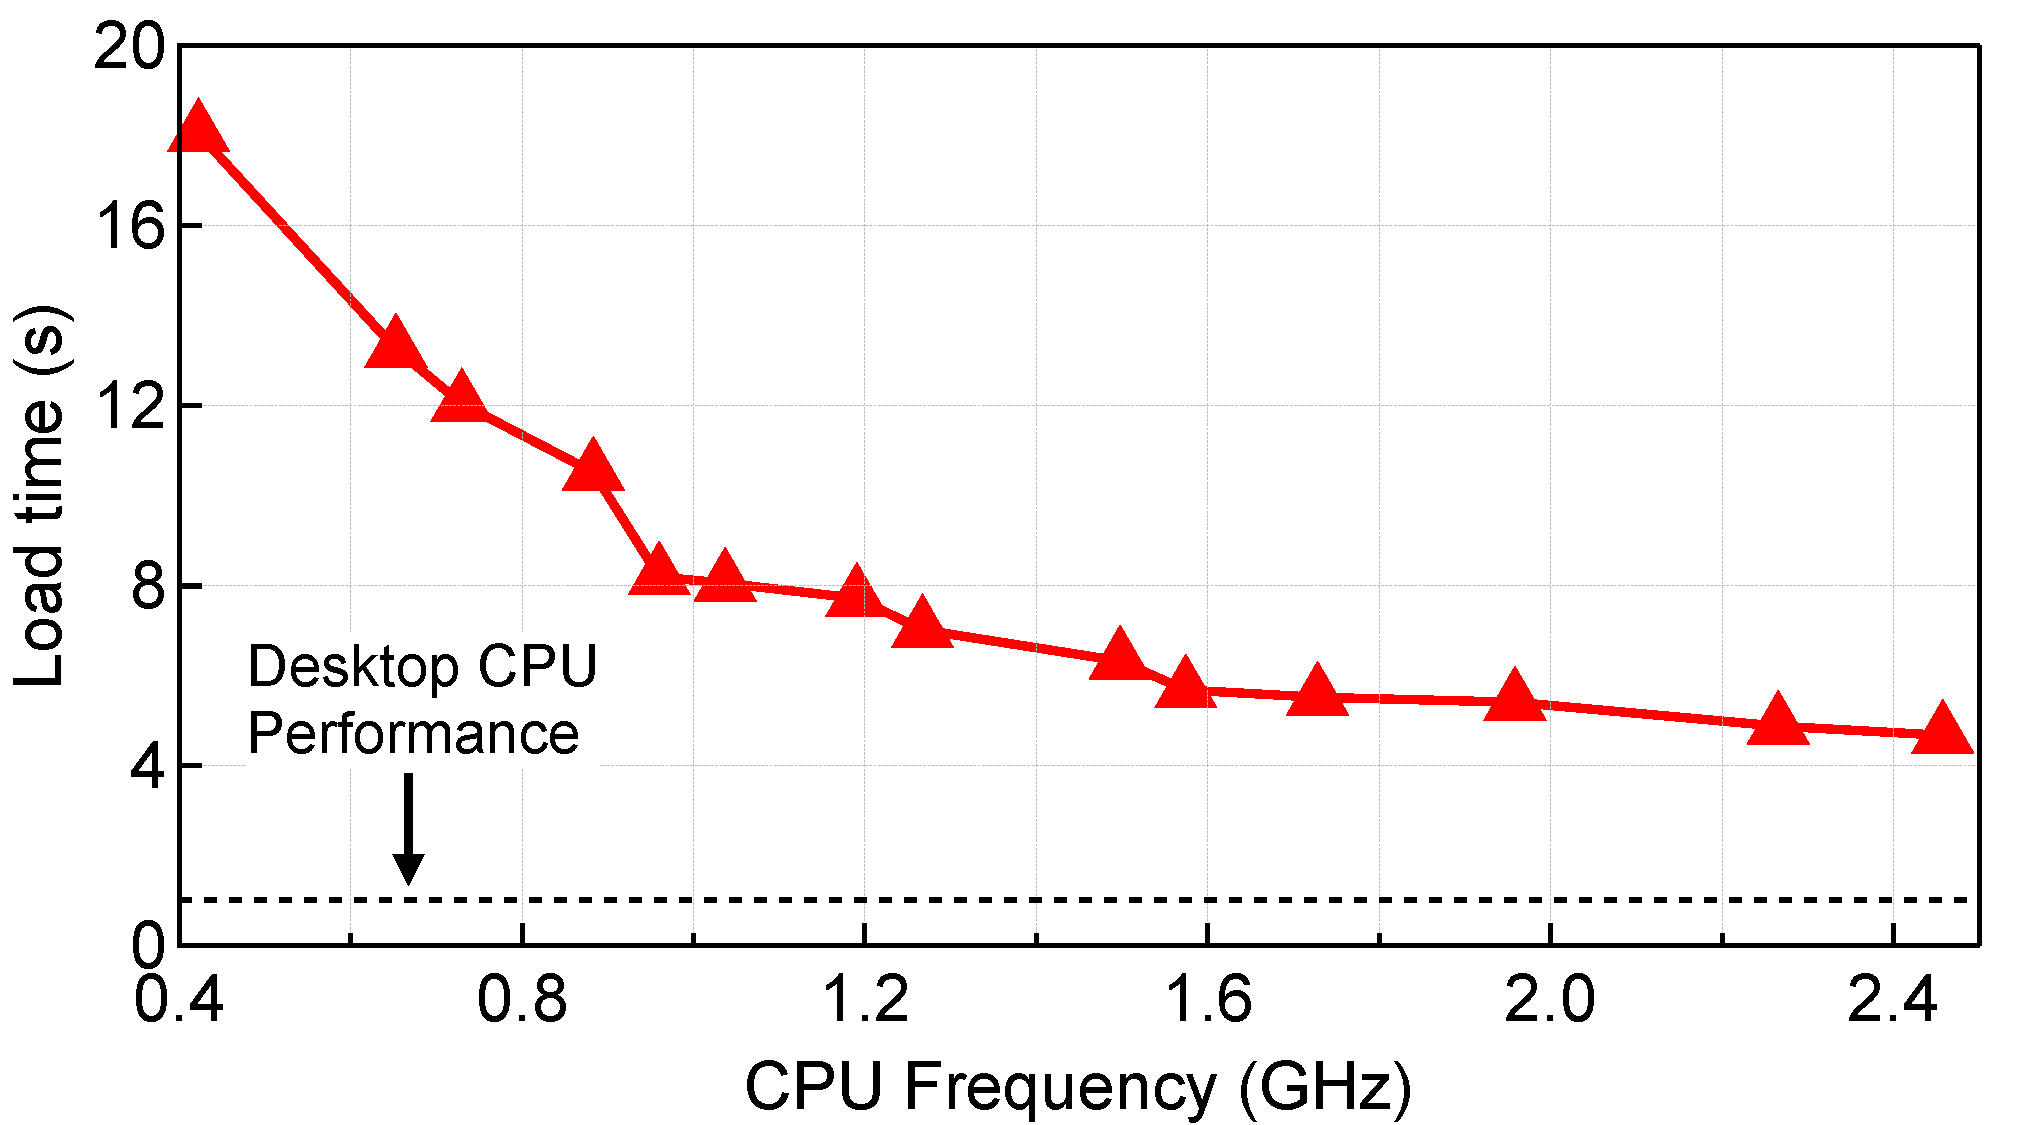
\includegraphics[trim=0 0 0 0, clip, width=\columnwidth]{cpu_bottleneck}
    \caption{Webpage load time with respect to CPU frequency on a Galaxy S5
smartphone. The markers represent CPU frequencies, which range from 0.4~GHz
(left) to 2.5~GHz (right). We also overlay the load time on a desktop CPU (the
dotted line) for comparison purpose.}
  \label{fig:cpu_bottleneck}
  \end{minipage}
\end{figure}

Note that increasing clock frequency between 1.6~GHz and 2.4~GHz yields small performance benefits. One may then naively conclude that mobile CPU performance improvements provide marginal improvements in Web performance. However, the ``marginal improvement'' is merely an artifact of using frequency as a performance proxy. At high frequencies, the processor's pipeline is already saturated, and the memory and interconnection become the microarchitectural-level bottlenecks~\cite{clockvsipc}. To overcome this artificial constraint and assess the impact of future mobile CPU improvements, we perform the same experiment on a desktop CPU (Intel Core i5 at 1.2~GHz). The result is shown as the dotted line in \Fig{fig:cpu_bottleneck}. The average webpage load time on the desktop CPU is about 1~second, effectively a 4X speedup over the peak performance of S5. This experiment shows that mobile CPU performance today is still far from reaching a diminishing return point, and it can continue to have a significant impact on mobile Web performance.

The takeaway from the results is that continuous improvement to network latency will eventually, if not already, take us to a point where further Web performance improvement will be unattainable without improving CPU performance.  This is a timely conclusion, especially when low latency cellular network, such as LTE, is already prevalent today. It is estimated that LTE's subscription will reach 1.37 billion (one-fifth of the world population) by the end of 2015~\cite{lte_subscription}.
%Note, however, that we do \emph{not} claim that network latency is irrelevant. When the network deviates from an ideal low-latency condition, or in emerging markets where high-latency network accesses are prevalent~\cite{em}, mobile Web performance is indeed constrained by the network latency.

\section{The Need for Energy-Efficient Computation in Mobile Web}
\label{sec:motivation:energy}

Despite the need for high-performance computation, mobile devices are severely limited by a battery-imposed energy budget, which in turn limits the achievable performance. In this section, I first use smartphones to quantitatively demonstrate that the energy budget of mobile devices is likely to stay stringently constrained in the near future. I then show that the CPU is becoming the worst power and energy consumer of a mobile device as compared to other components such as display and radio. There is clearly a need for energy-efficient computation in the mobile Web. Data presented here is adapted from the results of a related project~\cite{mobilecpu} that I collaborated on.

\paragraph{Energy Constraint} Battery technology has not experienced Moore's law-like improvements because of fundamental physics limitations~\cite{battery-mooreslaw}. As a result, the density of lithium-ion batteries has improved by only about 10\% per year~\cite{battery-stats}.  Therefore, the battery capacity of today's mobile devices is determined by the battery's volume, which is largely dictated by the device's screen size~\cite{phonescreen}. Using the smartphone as an example of a start-of-the-art mobile device, \Fig{fig:screen_batt} compares the screen sizes and battery capacities of over 600 smartphones from 2006 to 2014. There is a near-linear correlation between the battery capacity and screen size. As smartphone form factors reach maturity~\cite{phonesize}, the total device energy budget will likely stay severely constrained.

\begin{figure}[t]
\centering
  \begin{minipage}[b]{0.47\columnwidth}
    \centering
    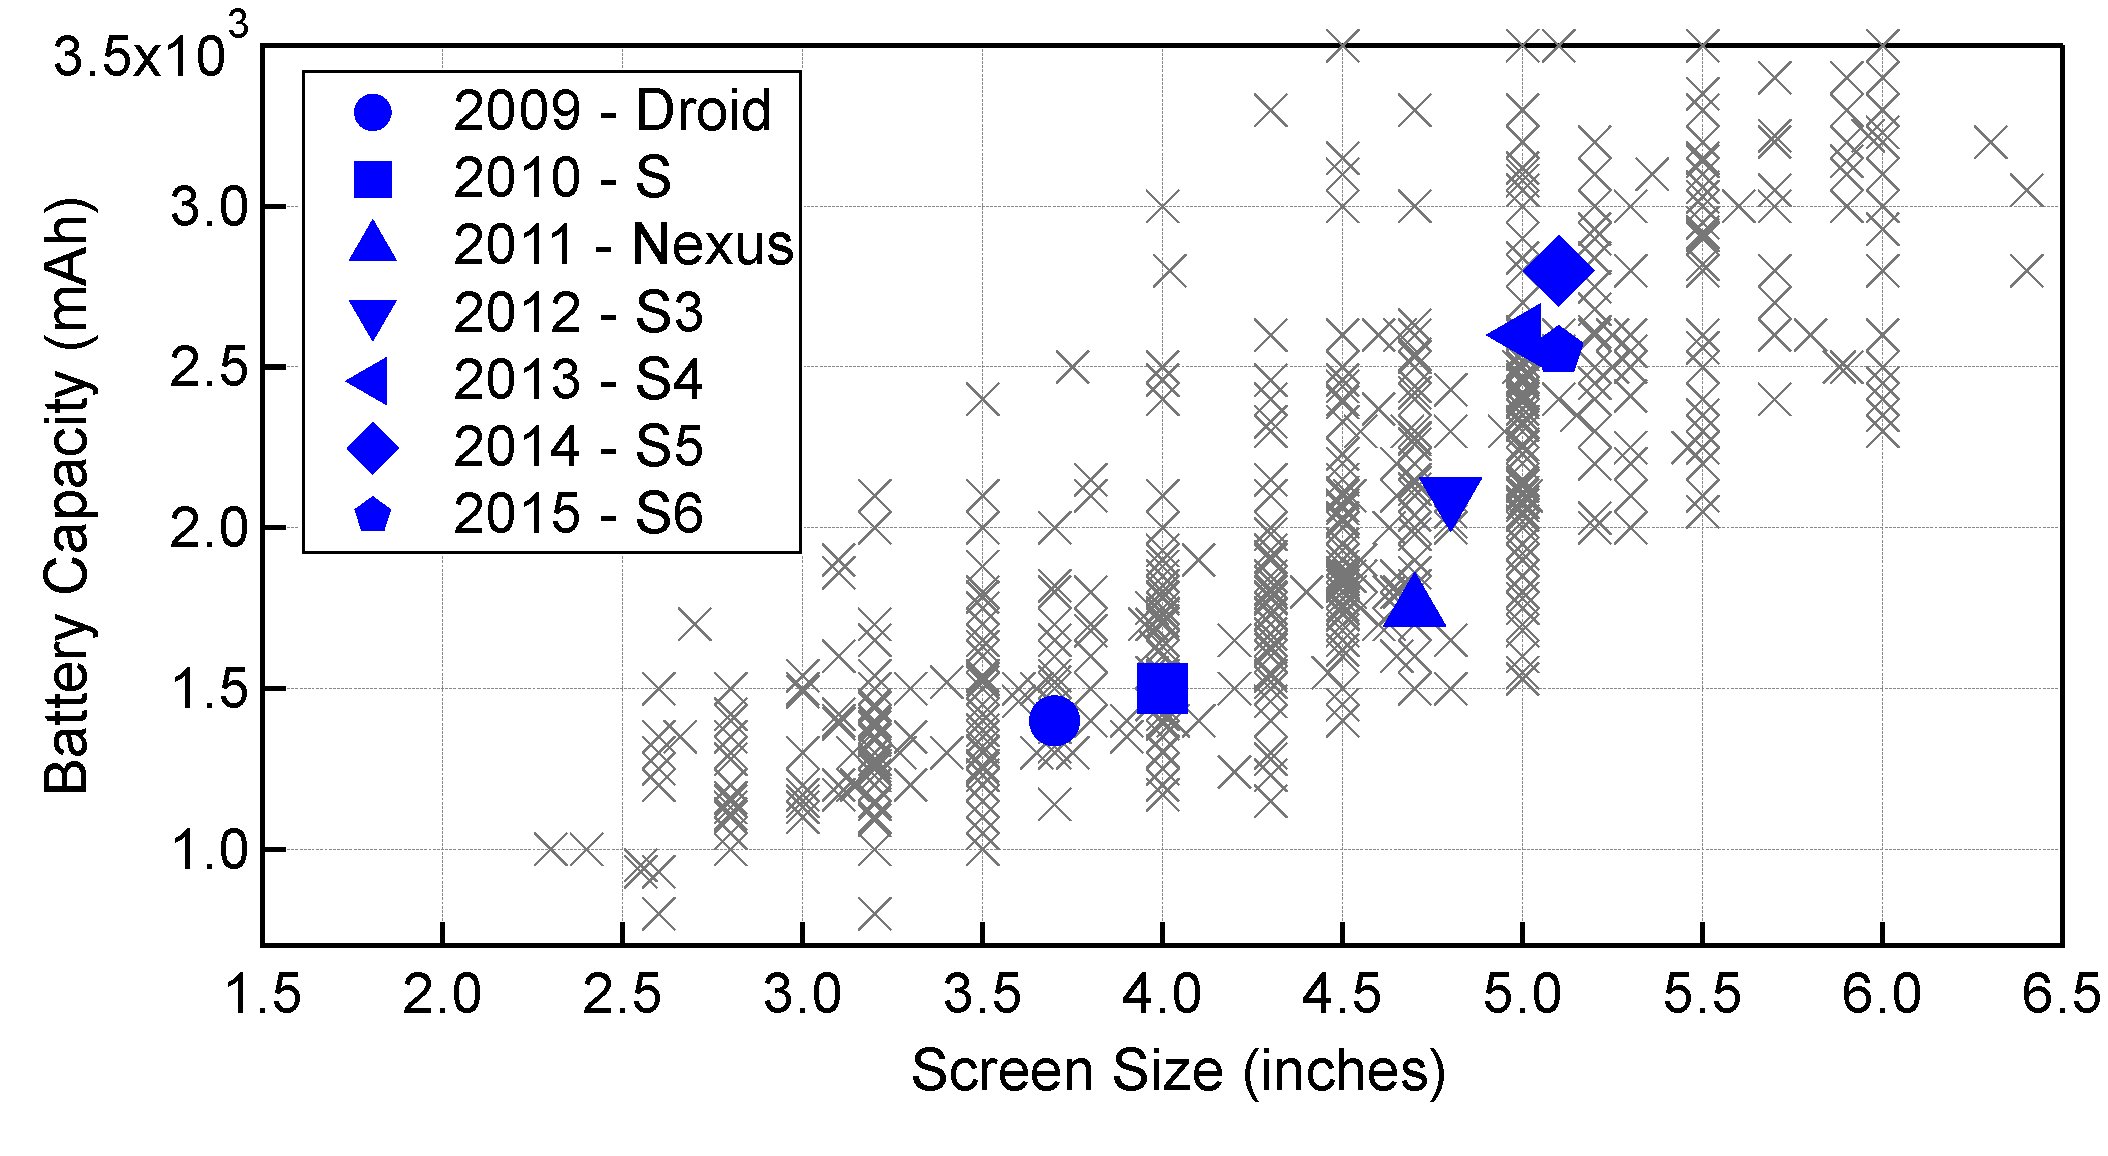
\includegraphics[trim=0 0 0 0, clip, width=\columnwidth]{figs/screen_batt}
    \caption{\small{There is an almost linear relationship between battery and screen size over the time.}}
  \label{fig:screen_batt}
  \end{minipage}
  \hspace*{15pt}
  \begin{minipage}[b]{0.47\columnwidth}
    \centering
    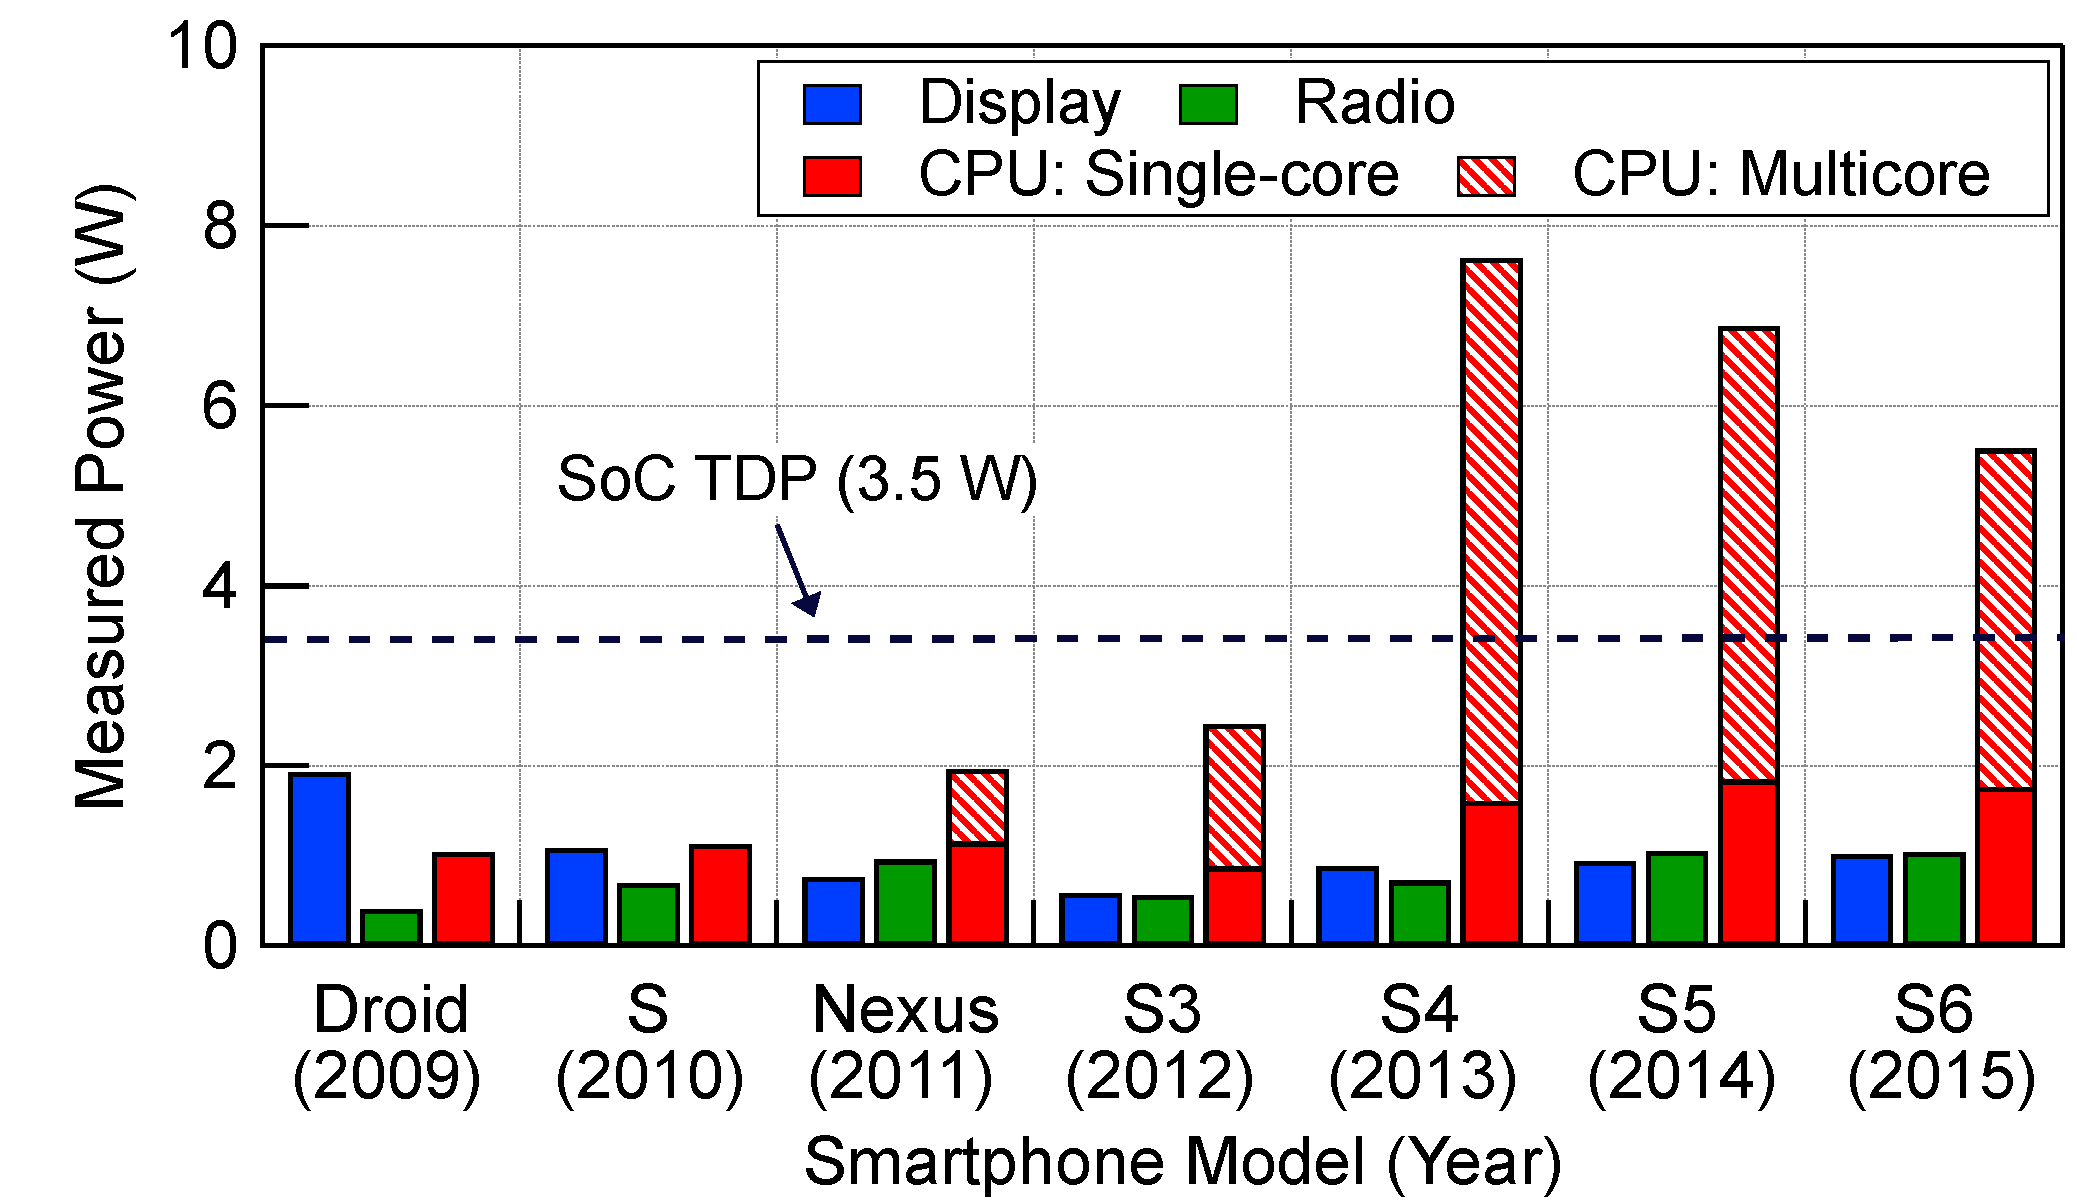
\includegraphics[trim=0 0 0 0, clip, width=\columnwidth]{figs/phone_power_trend}
    \caption{\small{CPU power consumption has increased significantly compared to other key components.}}
  \label{fig:phone_power_trend}
  \end{minipage}
\end{figure}

\paragraph{Mobile CPU's Rise to Power} Different components contribute to the overall power consumption of a mobile device. \Fig{fig:phone_power_trend} compares the measured power consumption of three major mobile device components: CPU, display, and radio. We select seven top smartphones for each year from 2009 to 2015. They are Motorola's Droid from 2009, and Samsung's Galaxy S, Nexus, S3, S4, S5, and S6 from 2010 through 2015, respectively. Chronologically, the seven phones represent how cutting-edge smartphone technologies have progressed over time. The results are collected while running a standard Web benchmark, Sunspider~\cite{sunspider}, for the CPU(s), and dedicated benchmarks for the other components~\cite{carroll2010analysis, ookla}. We used the Monsoon power monitor to measure the seven smartphones' power consumptions at the battery level.

We make two important observations from~\Fig{fig:phone_power_trend}. First of all, CPU is now a major power consumer of a mobile device. The year 2011 marks an inflection point where a single CPU core began overtaking the display as the most power consuming component. On any of the last three mobile CPU generations, the multicore CPU can exceed the entire mobile device's thermal design power~(TDP) even without including the radio and display's power consumptions.

Second, while other components are becoming more power-efficient over time due to technological advancements~\cite{chen2013energy}, the CPU's power has risen sharply. The excessive mobile CPU power consumption is a direct result of current mobile CPU design strategy, i.e., merely adopting desktop-like design techniques such as aggressive single-core microarchitecture enhancement and multicore scaling to improve performance~\cite{mobilecpu}. As the Dennard Scaling~\cite{dennard} comes to its end, the performance benefits do not sufficiently make up for the additional power consumption~\cite{mobilecpu}, eventually hurting mobile CPU's energy-efficiency.
%For example, I observed that the energy consumption improvement of Web browsing has already plateaued since 2012~\cite{zhu2015role}.
%A recent measurement study further suggests that the CPU contributes to about 50\% of the total device energy consumption for various mobile Web applications~\cite{mobilebench}.

Given that users expect each mobile device generation to incorporate new peripherals such as sensors that also require energy from the same budget, it is clear that the CPU, as a major energy consumer, needs to become more energy-efficient while sustaining performance improvement.


%!TEX root=../paper.tex

\chapter{WebCore: A Mobile Processor Architecture Substrate for Web Computing}
\label{sec:arch}

Domain-specific specialized architecture has long been deemed as extremely high-performance and energy-efficient because it aggregates hundreds of operations in a few instructions and, therefore, reduces major sources of inefficiencies in general-purpose CPUs~\cite{h264,soda,anysp}. The key challenge of applying architectural specialization to Web computing is how to \textit{retain general-purpose programmability}. The general-purpose programmability is a particular necessity for Web technologies because they involve large pieces of software that are written in a combination of different general-purpose programming languages. For example, Google's Chrome Web browser is developed in 29 languages with over 17 million lines of code~\cite{chromeloc}. Recent work has demonstrated the importance and feasibility of balancing general-purpose programmability and specialization in various data computation domains (e.g., H.264 encoding~\cite{h264}, convolution~\cite{ce}).

%Following the architecture design philosophy of balancing general-purpose programmability and domain-specific specialization, I propose the \webcore, a general-purpose CPU customized and specialized for Web technologies. \webcore's design starts from existing mobile CPUs, and thus retains the general-purpose programmability. It achieves performance and energy improvement by combining customization and specialization techniques. In the rest of this section, I describe the customization and specialization process in \Sect{sec:arch:customization} and \Sect{sec:arch:specialization}, respectively. \Sect{sec:arch:related} puts \webcore in the context of prior work on hardware support for the mobile Web.

Following the architecture design philosophy of balancing general-purpose programmability and domain-specific specialization, we propose \webcore, \textit{a general-purpose core customized and specialized for mobile Web computing}. In comparison to prior work that either takes a fully software approach on general-purpose processors~\cite{zoomm,ParallelBrowser} or a fully hardware specialization approach~\cite{SiChrome}, our design strikes a balance between the two. On one hand, \webcore retains the flexibility and programmability of a general-purpose core. It naturally fits in the multicore SoC that is already common in today's mainstream mobile devices. On the other hand, it achieves energy-efficiency improvement via modest hardware specializations that create closely coupled datapath and data storage.

We begin by examining existing general purpose designs for the mobile Web applications. Through exhaustive design space exploration, we find that existing general purpose designs bear inherent sources of energy-inefficiency. In particular, instruction delivery and data feeding are two major bottlenecks. We show that customizing current designs by properly sizing key design parameters achieves better energy efficiency. The customization step ensures that further optimizations are performed upon an optimized general-purpose baseline.

Building on the customized general-purpose baseline, we develop specialized hardware to further overcome the instruction delivery and data feeding bottlenecks. We propose two new optimizations: the \emph{``Style Resolution Unit''} (SRU) and a \emph{``Software-Managed Browser Engine Cache.''} The SRU is a hardware accelerator for the critical style-resolution kernel within the Web browser engine. It is based on the observation that the style-resolution kernel has abundant fine-grained parallelism that is hidden in a software implementation but can be captured by a dedicated hardware structure. SRU employs a GPU-like multi-lane architecture to exploit the inherent parallelism. Through exploiting the parallelism, the SRU aggregates enough computations in a few operations, which effectively increases the arithmetic intensity and offsets the instruction delivery and data feeding overhead.

The proposed browser engine cache structure improves data feeding efficiency by exploiting the unique data access pattern of the browser engine's principal data structures such as the DOM tree and the Render tree. Web applications typically operate on one DOM/Render tree node heavily and traverse to the next one, indicating both heavy data reuse and predictable access pattern. The browser engine cache uses a small and energy-conserving hardware memory to capture the heavy data reuse and uses software to predict the access pattern and to manage the cache. Overall, the browser cache achieves a high hit rate for the important data structures but with extremely low accessing energy.

Our results show that customizations alone on the existing general-purpose mobile processor design lead to 22.2\% performance improvement and 18.6\% energy saving. Our specialization techniques achieve an additional 9.2\% performance improvement and 22.2\% overall energy saving; the accelerated portion itself achieves up to 10X speedup. Finally, we also show that our specialization incurs negligible area overhead. More importantly, such overhead, if dedicated to tuning already existing general-purpose architectural features (e.g., caches), lead to much lower energy-efficiency improvements.

The rest of the paper is organized as follows. We first describe our experimental setup including software/hardware infrastructure and application selection in \Sect{sec:arch:exp}. We then describe the design-space explorations that allow us to identify sources of inefficiency in existing general-purpose processors and customize them for mobile Web applications in \Sect{sec:arch:customization}. Building on top of the customized general-purpose designs, we further propose the two new specialization techniques in \Sect{sec:arch:sru} and \Sect{sec:arch:cache}. We show that our proposed \webcore achieves significant performance and energy-efficiency improvement over existing designs in \Sect{sec:arch:eval}. We review related work in \Sect{sec:arch:related}.

\section{Experimental Setup}
\label{sec:arch:exp}

Before we begin our investigation, we describe our software infrastructure, specifically outlining our careful selection of representative webpages to study, and the processor simulator. 

\paragraph{Web Browser} We focus on the popular WebKit~\cite{webkit} rendering engine used in Google Chromium (Version 30.0) for our studies. WebKit is also widely used by other popular mobile browsers, such as Apple's Safari and Opera.

\paragraph{Benchmarked Web Applications}  We pay close attention to the choice of webpages to ensure that the WebCore design is not misled. We mine through the top 10,000 websites as ranked by Alexa~\cite{alexa} and pick the 12 most representative websites. All except one happen to rank among Alexa's top 25 websites. The 12 benchmarked websites also cover 10 of BBench's 11 webpages~\cite{BBench}. \Sect{sec:arch:eval} lists the website names. We refer interested readers to \Sect{sec:arch:related:char} for a discussion of BBench. 

\begin{figure}[t]
  \centering
  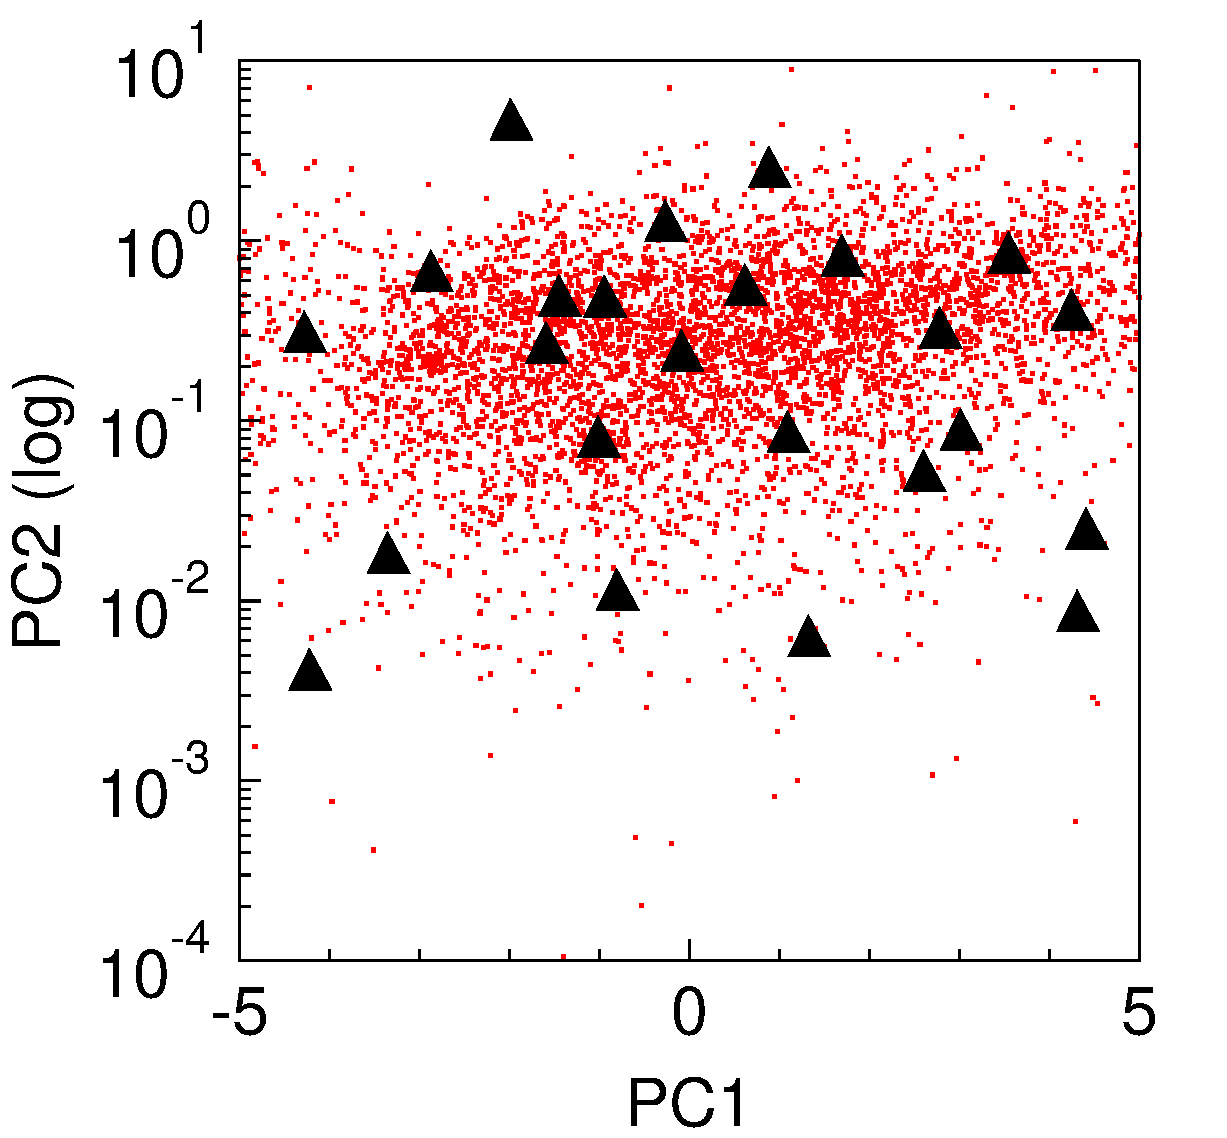
\includegraphics[trim=0 0 0 0, clip, width=.55\columnwidth]{pca}
  \caption{We pick 24 representative webpages from 10,000 of the hottest webpages as per \texttt{www.alexa.com}}
  \label{fig:pca}
\end{figure}

We consider not only the mobile version of the 12 websites, but also their desktop counterparts. Many mobile users still prefer desktop-version websites for their richer content and experience~\cite{Slocum:2011fk,Bixby:2011uq}. Moreover, many mobile devices, especially tablets, typically load the desktop version of webpages by default. As webpage sizes exceed 1~MB~\cite{Everts:2011kx}, we must study mobile processor architectures that can process more complex content and not just simple mobile webpages.

We study 24 distinct webpages in total. The 24 benchmarked webpages are representative because they capture the webpage variations in both webpage-inherent and microarchitecture-dependent features. To prove this, we performed principal component analysis (PCA), which is a statistical method that reduces the number of inputs without losing generality~\cite{PCA}.  PCA transforms the original inputs into a set of principal components (PC) that are linear combinations of the inputs. In our study, PCA calculates four PCs from about 400 distinct features. These four PCs account for 70\% of the variance across all of the original 10,000 webpages. \Fig{fig:pca} shows the results for two major components, PC1 and PC2. IPC (microarchitecture-dependent feature) is the single most significant metric in PC1, and the number of DOM tree nodes (webpage-inherent feature) is the most significant metric in PC2. The triangular dots represent our webpages. They cover a very large spread of the top 10,000 webpages in the Internet.

\paragraph{Performance Metric} We focus on the initial loading of Web applications. This is because user QoS experience is strongly tied to the initial load time in Web applications. For instance, it is estimated that 79\% of online shoppers will not return to the website with slow load time~\cite{Jacob:2013fk}.

Unless stated otherwise, we define Web application load time as the execution time that elapses until the~\texttt{onload} event is triggered by the Web browser. It is worth noting that during the loading phase (i.e., before the \texttt{onLoad} event is triggered), many Web applications execute JavaScript code such as Ads and analytics. Therefore, our study not only takes into account the initial loading of the webpage, but also includes JavaScript activity that is triggered automatically by Web applications.

\paragraph{Simulators} We assume the x86 instruction set architecture (ISA) for our study. Prior work shows that the ISA does not significantly impact energy efficiency for mobile workloads~\cite{risc-cisc}. Therefore, we believe that our microarchitecture explorations are generally valid across ISAs. We use Marss86~\cite{marss}, a cycle-accurate simulator, in full-system mode to faithfully model all the network and OS activity. Performance counters from Marss86 are fed into McPAT~\cite{mcpat} for power estimation.

%We do our best-effort validation of the simulator by comparing it with an ARM platform because we do not have access to a measurable x86 mobile platform. We use the ODroid XU+E development board~\cite{odroidxue} that hosts the Exynos 5410 SoC as the hardware platform. The Exynos 5410 SoC is known for powering the Samsung's Galaxy S4 smartphone. The Exynos 5410 SoC contains an ARM Cortex-A15 processor. In our measurements, single core Cortex-A15 consumes 1.7~J energy and 2~seconds to load~\website{www.cnn.com}. For comparison, we tune our simulator configurations to best match the microarchitecture parameters of Cortex-A15. The simulation results report 1.2~J and 2.2~seconds for energy consumption and loading time, respective.

\section{Customizing General-Purpose Cores}
\label{sec:arch:customization}

\webcore design is based on general-purpose CPUs to best retain the general-purpose programmability. However, existing general-purpose processors may not be an ideal baseline for \webcore, because they are not uniquely tuned for Web applications. \webcore customizes current designs by exploring a vast design space to properly size key microarchitecture parameters (\Sect{sec:arch:customization:dse}). I derive two major conclusions through the customization process. First, out-of-order designs provide more flexibility for energy versus performance trade-offs than in-order designs (\Sect{sec:arch:customization:core}). Second, a customized out-of-order design configuration still contains two sources of inefficiency--instruction delivery and data feeding--that need to be further mitigated (\Sect{sec:arch:customization:sources}).

\subsection{Design Space Exploration}
\label{sec:arch:customization:dse}

\paragraph{Design Space Specification} We define the set of tunable microarchitectural parameters in \Tbl{tab:dse:para}. We vary the values of functionally related parameters (e.g., issue width and the number of functional units) together to avoid reaching an entirely unbalanced design~\cite{ilp2}. We also do not consider single-issue out-of-order processors, which are known to be energy inefficient~\cite{marginal}. In total, we consider over 3~billion design points.

%!TEX root=../../paper.tex

\begin{table}[p]
\large
\centering
\captionsetup{width=.9\columnwidth}
\caption{Microarchitecture design-space parameters. The first column shows the parameters that are considered in our DSE. The second column shows the metric that the value of each parameter is measured. The $i$::$j$::$k$ in the third column denotes values ranging from $i$ to $k$ at steps of $j$}
\renewcommand*{\arraystretch}{1.4}
\renewcommand*{\tabcolsep}{25pt}
\resizebox{.9\columnwidth}{!}
{
	\begin{tabular}{l l l l l l}
	\toprule[0.15em]
		\bigstrut\textbf{Parameters} & \bigstrut\textbf{Measure} & \bigstrut\textbf{Range}\\
	\midrule[0.05em]
		Issue width				&	count					&	1::1::4	\\
		\# Functional units		&	count					&	1::1::4 \\
		%I-TLB size				&	\#entries				&	8::8::32 \\
		%D-TLB size				&	\#entries				&	8::8::32 \\
		Load queue size			&	\# entries				&	4::4::16 \\
		Store queue size		&	\# entries				&	4::4::16 \\
        Branch prediction size  &   $log_{2}$(\#entries)    &   1::1::10\\
		ROB size				&	\# entries				&	8::8::128 \\
		\# Physical registers	&	\# entries				&	5::5::140 \\
		L1 I-cache size			&	$log_{2}$(KB)			&	3::1::7 \\
		L1 I-cache delay		&	cycles					&	1::1::3 \\
		L1 D-cache size			&	$log_{2}$(KB)			&	3::1::7 \\
		L1 D-cache delay		&	cycles					&	1::1::3\\
		L2 cache size			&	$log_{2}$(KB)			&	7::1::10 \\
		L2 cache delay			&	cycles					&	16,32,64 \\
	\bottomrule[0.15em]
	\end{tabular}
}
\label{tab:dse:para}
\end{table}


We intentionally relax the design parameters beyond the current mobile systems in order to allow an exhaustive design space exploration. For example, we consider up to 128~KB L1 cache design whereas most L1 caches in existing mobile processors are 32~KB in size. Also, since thermal design power (TDP) is important for mobile SoCs, we eliminate overly aggressive designs with more than 2~W TDP.

We assume a fixed core frequency in our design-space exploration. We use 1.6~GHz, a common value in mobile processors~\cite{snapdragon-wiki,exynos-wiki}, to further prune the exploration space. However, because the latency of both the L1 and L2 caches can still vary, we include different cache designs in the exploration space.

We use a constant memory latency to model the memory subsystem because we do not observe significant impact of the memory system on the mobile Web browsing workload. According to hardware measurements on the Cortex-A15 processor using ARM's performance monitoring tool Streamline~\cite{streamline}, the MPKI for the L2 cache across all the webpages is below 5. We observe similar low L2 MPKI, i.e. low main memory pressure, in our simulations. Therefore, we use a simpler memory system to further trim the search space.

\paragraph{Statistical Inference Method} It is not feasible to simulate billions of the design points that we consider simply due to time constraints. Therefore, we leverage the statistical inference technique that trains predictive models using a small number of samples. Such models reflect how different microarchitecture parameters, both individually and collectively, influence performance and power consumption. Statistical inference methods have been used successfully in the past for architecture design-space exploration~\cite{dse,comt}.

In particular, we use linear regression modeling~\cite{RMS} to construct our predictive models. A linear regression model can be formulated as in~\Equ{equ:linear}, where $y$ denotes the response, $x = x_{1},...,x_{p}$ denote \textit{p} predictors, and $\beta = \beta_{0},...,\beta_{p}$ denote corresponding coefficients of each predictor. The \textit{least squares method} is used to solve the regression model by identifying the best-fitting $\beta$ that minimizes the residual sum of squares (RSS)~\cite{ESL}. In our case, the response $y$ is either performance (measured in terms of instruction per cycle, IPC) or power, and the predictors $x_{i}$ are microarchitecture structures listed in \Tbl{tab:dse:para}.

\begin{equation}
       y = \beta_0 + \sum_{i=1}^{p} x_i \beta_i
\label{equ:linear}
\end{equation}

We find that 2,000 \textit{uniformly at random} (UAR) samples of microarchitecture configurations from the design space are sufficient in our case to construct robust models. We also obtain 500 additional UAR samples from the cache design space (both L1 and L2) to reinforce the credibility of instruction and data cache design predictions. We perform cross-validation of the model (i.e., we partition a sample dataset into complementary subsets, and perform analysis on one subset and validate the analysis on the other subset), and then obtain additional samples from the design space for full evaluation.

\begin{figure}[t]
  \centering
  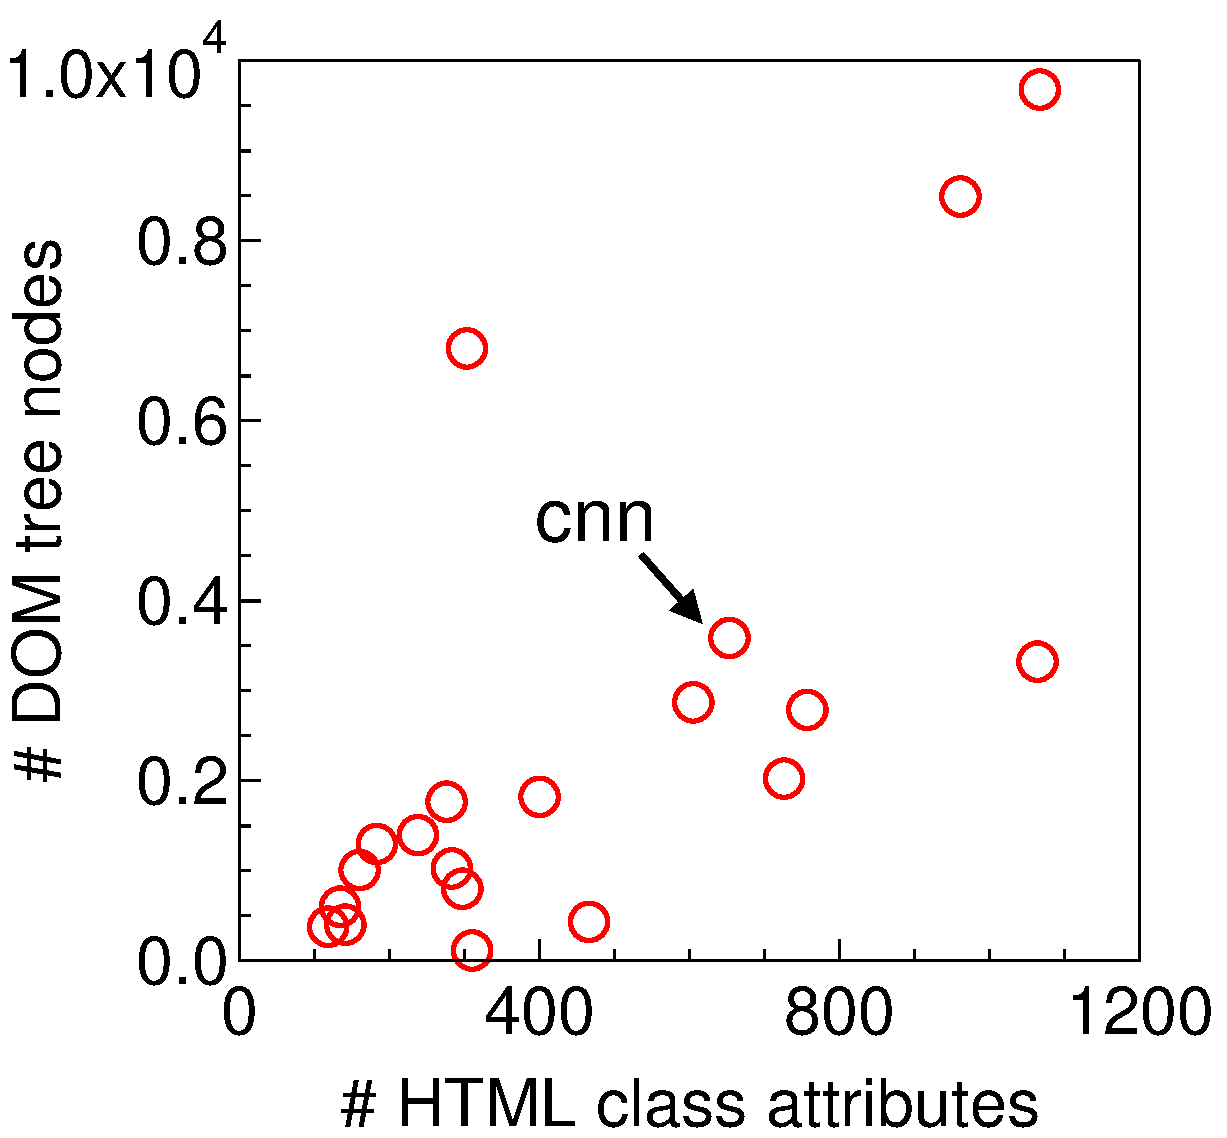
\includegraphics[trim=0 0 0 0, clip, width=.55\columnwidth]{cnn}
  \caption{\website{www.cnn.com} is a representative webpage from our benchmark suite because it is almost the centroid.}
  \label{fig:cnn}
\end{figure}

In order to derive general conclusions about the design space and optimize for the common case, in this section we present only our in-depth analysis for the representative website \website{www.cnn.com}. ~\Fig{fig:cnn} compares~\website{www.cnn.com} with other webpages to demonstrate that it is indeed representative of the other benchmarked webpages. The $x$-axis and $y$-axis represent the number of DOM tree nodes and the number of~\textsf{class} attributes in HTML. These are the two webpage characteristics that are most correlated with a webpage's load time and energy consumption~\cite{big-little}. As the figure shows,~\website{www.cnn.com} is roughly the centroid of the benchmarked webpages, and thus we use it as a representative webpage for the common case.

We construct predictive models for out-of-order and in-order design space separately because microarchitecture structures have different impact on performance and power in in-order and out-of-order pipelines. In general, the out-of-order models' error rates are below 6.0\%. The in-order models (not shown) are more accurate because of their simpler design. On average, the in-order performance and power models' errors are within 5\% and 2\%, respectively.

\begin{figure}[t]
  \centering
  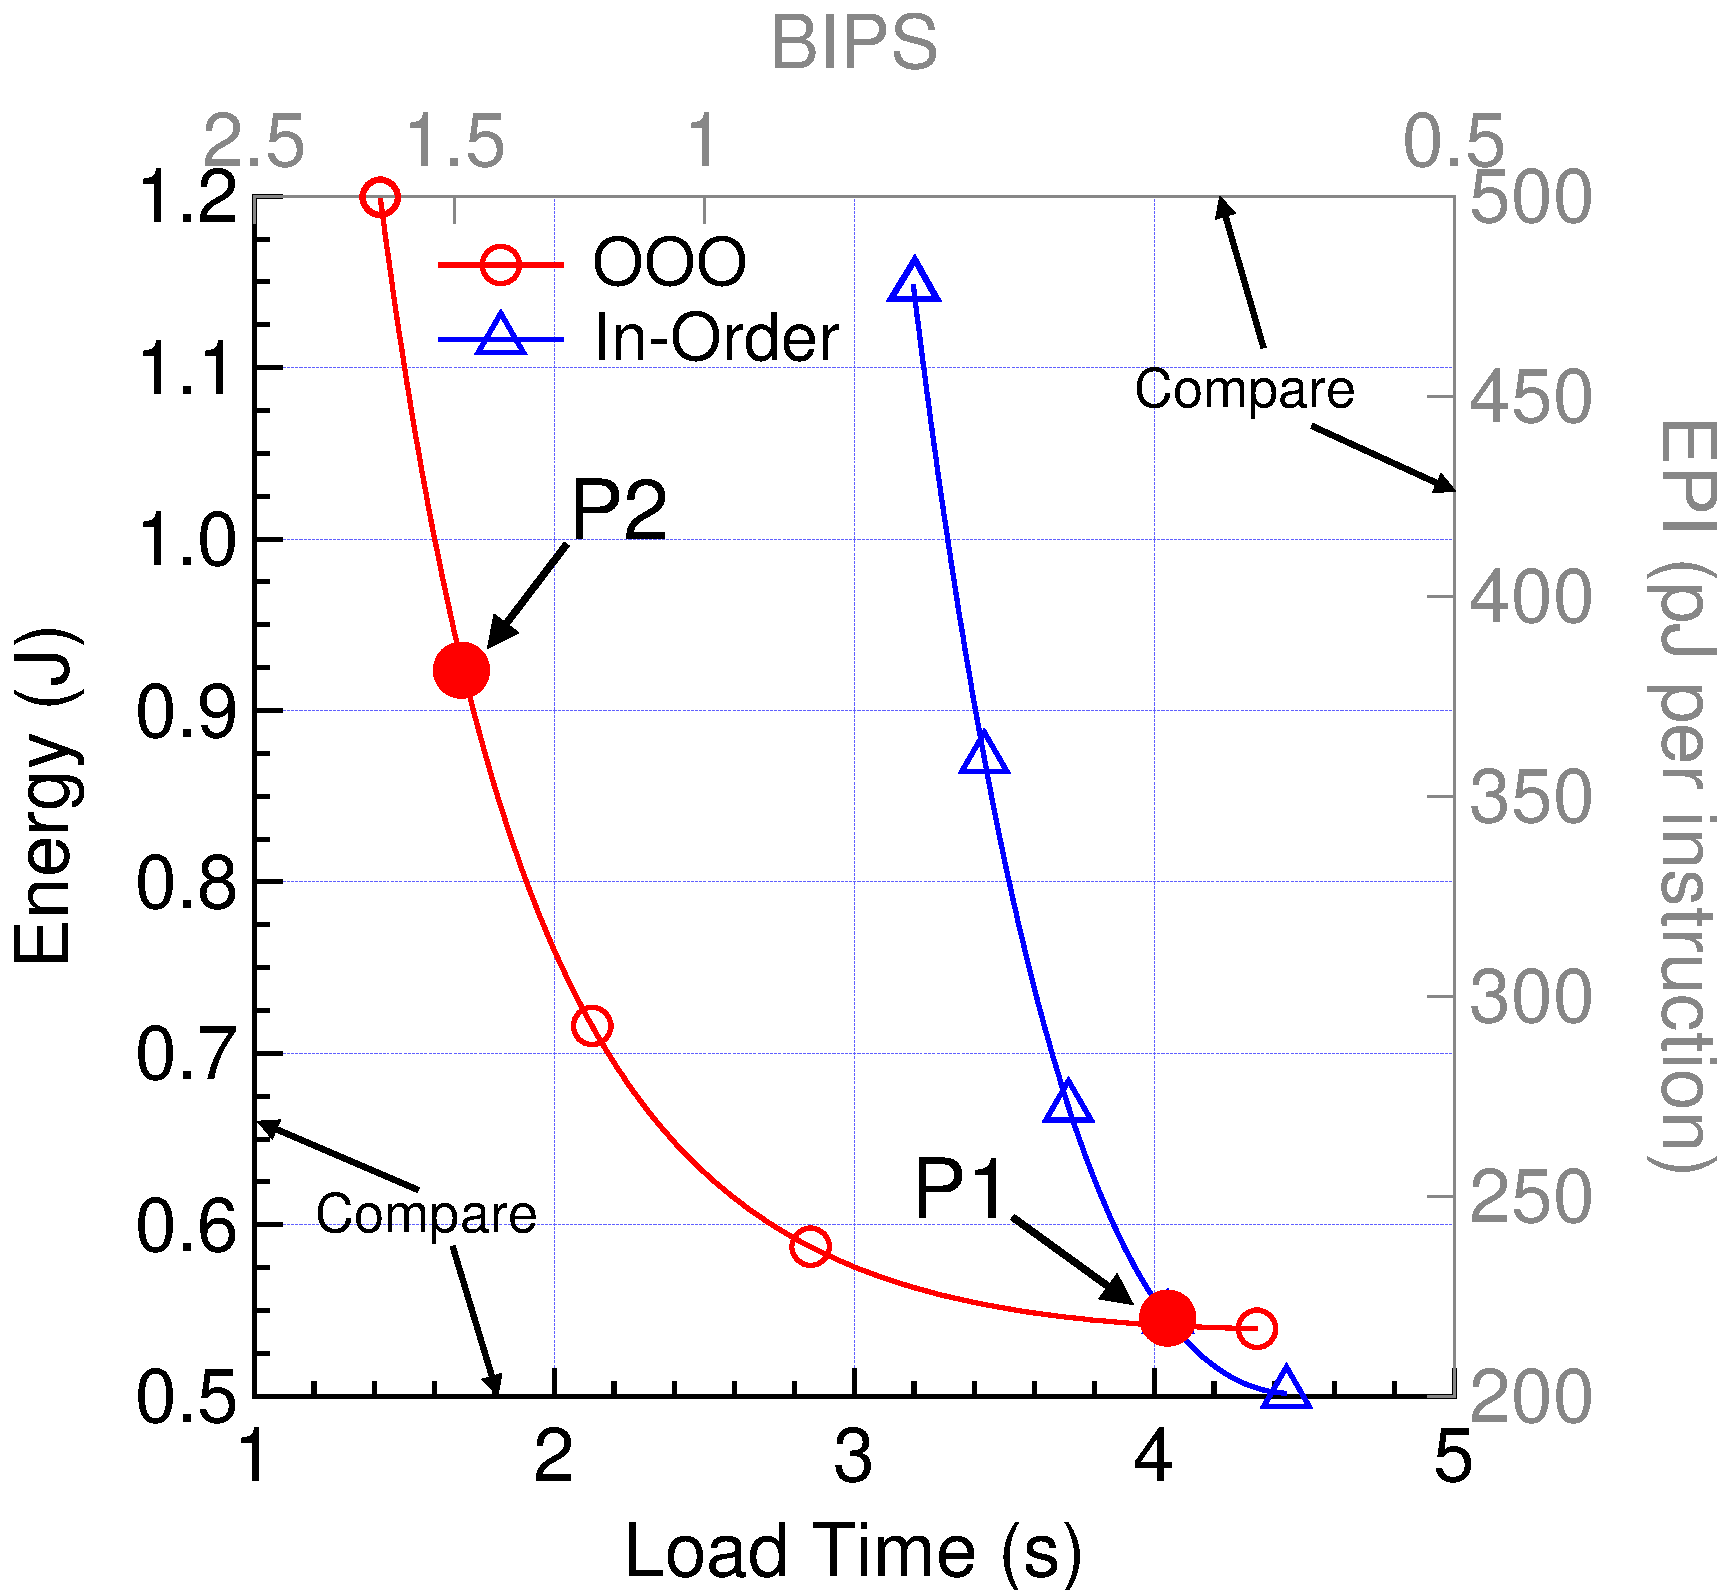
\includegraphics[trim=0 0 0 0, clip, width=.6\columnwidth]{ivso}
  \caption{In-order versus out-of-order Pareto optimal frontiers.}
  \label{fig:ivso}
\end{figure}

\subsection{In-order vs. Out-of-order Design Space Exploration}
\label{sec:arch:customization:core}

Design space exploration helps customization at the ``macro-architecture'' level, i.e., determining between in-order and out-of-order designs. We understand the difference between in-order and out-of-order design space by examining their Pareto optimal frontiers. Design points on a Pareto optimal frontier reflect different optimal design decisions given specific performance/energy targets. The Pareto-optimal is more general than the (sometimes overly specific) $EDP$, $ED^{2}P$ metrics, etc. Design configurations optimized for such metrics have been known to correspond to different points on the Pareto-optimal frontier~\cite{marginal}. \Fig{fig:ivso} shows the Pareto-optimal frontiers of both in-order and out-of-order designs between energy and performance. We use energy per instruction (EPI) for the energy metric, and million instructions per second (MIPS) as the performance metric. 

We make two important observations from \Fig{fig:ivso}. First, the out-of-order design space offers a much larger performance range ($\sim$1~BIPS between markers P1 and P2, see top $x$-axis) than the in-order design space (\textless~0.5~BIPS), which reflects the out-of-order's flexibility in design decisions. Second, the out-of-order design frontier is flatter around the 4-second webpage load time range (see marker P1) than in the in-order design, which indicates that the out-of-order design has a much lower marginal energy cost. The observation indicates that processor architects can make design decisions based on the different performance goals without too much concern about the energy budget. In contrast, the in-order design space quickly enters the region of diminishing returns (i.e., sharp increase in energy consumption) as we push toward webpage load times that are less than 4 seconds. In other words, the in-order design has a low marginal performance value (or equivalently high marginal cost of energy).

%\Fig{fig:ivso} shows the Pareto optimal frontiers of the in-order and out-of-order design space. We observe that the in-order design space has a narrow performance range of 1~second, whereas the out-of-order space covers a 4~second performance range. The performance range contrast indicates that out-of-order designs can more flexibly balance performance with energy and, therefore, are better design baselines for mobile Web applications.

\begin{figure}[t]
  \centering
  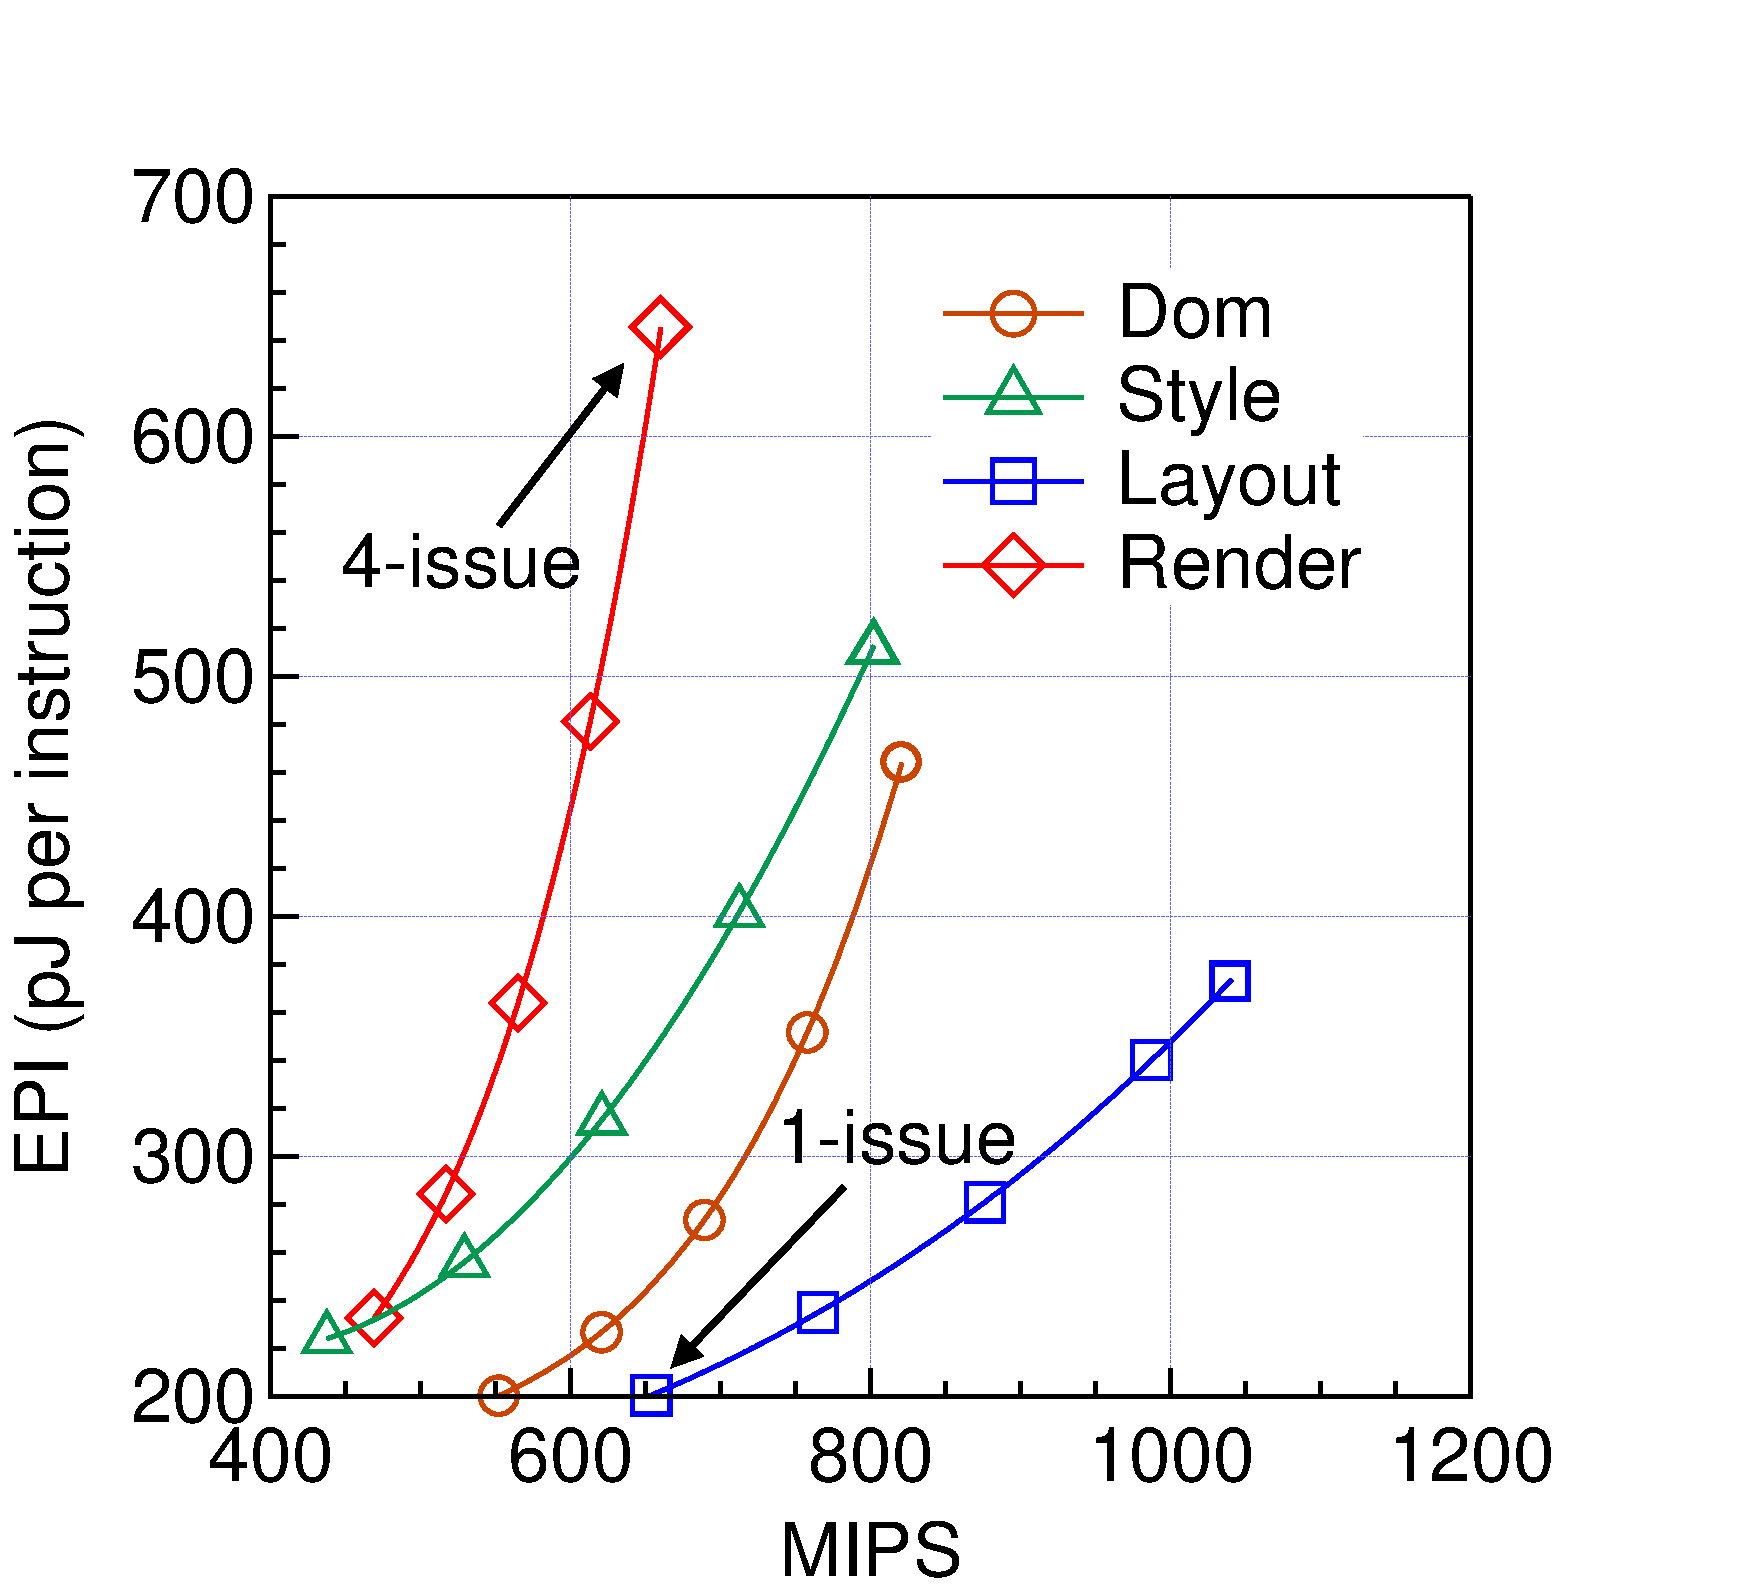
\includegraphics[trim=0 0 0 0, clip, width=.6\columnwidth]{pareto_io}
  \caption{In-order Pareto optimal frontier for each kernel.}
  \label{fig:pareto_io}
\end{figure}

\begin{figure}[t]
  \centering
  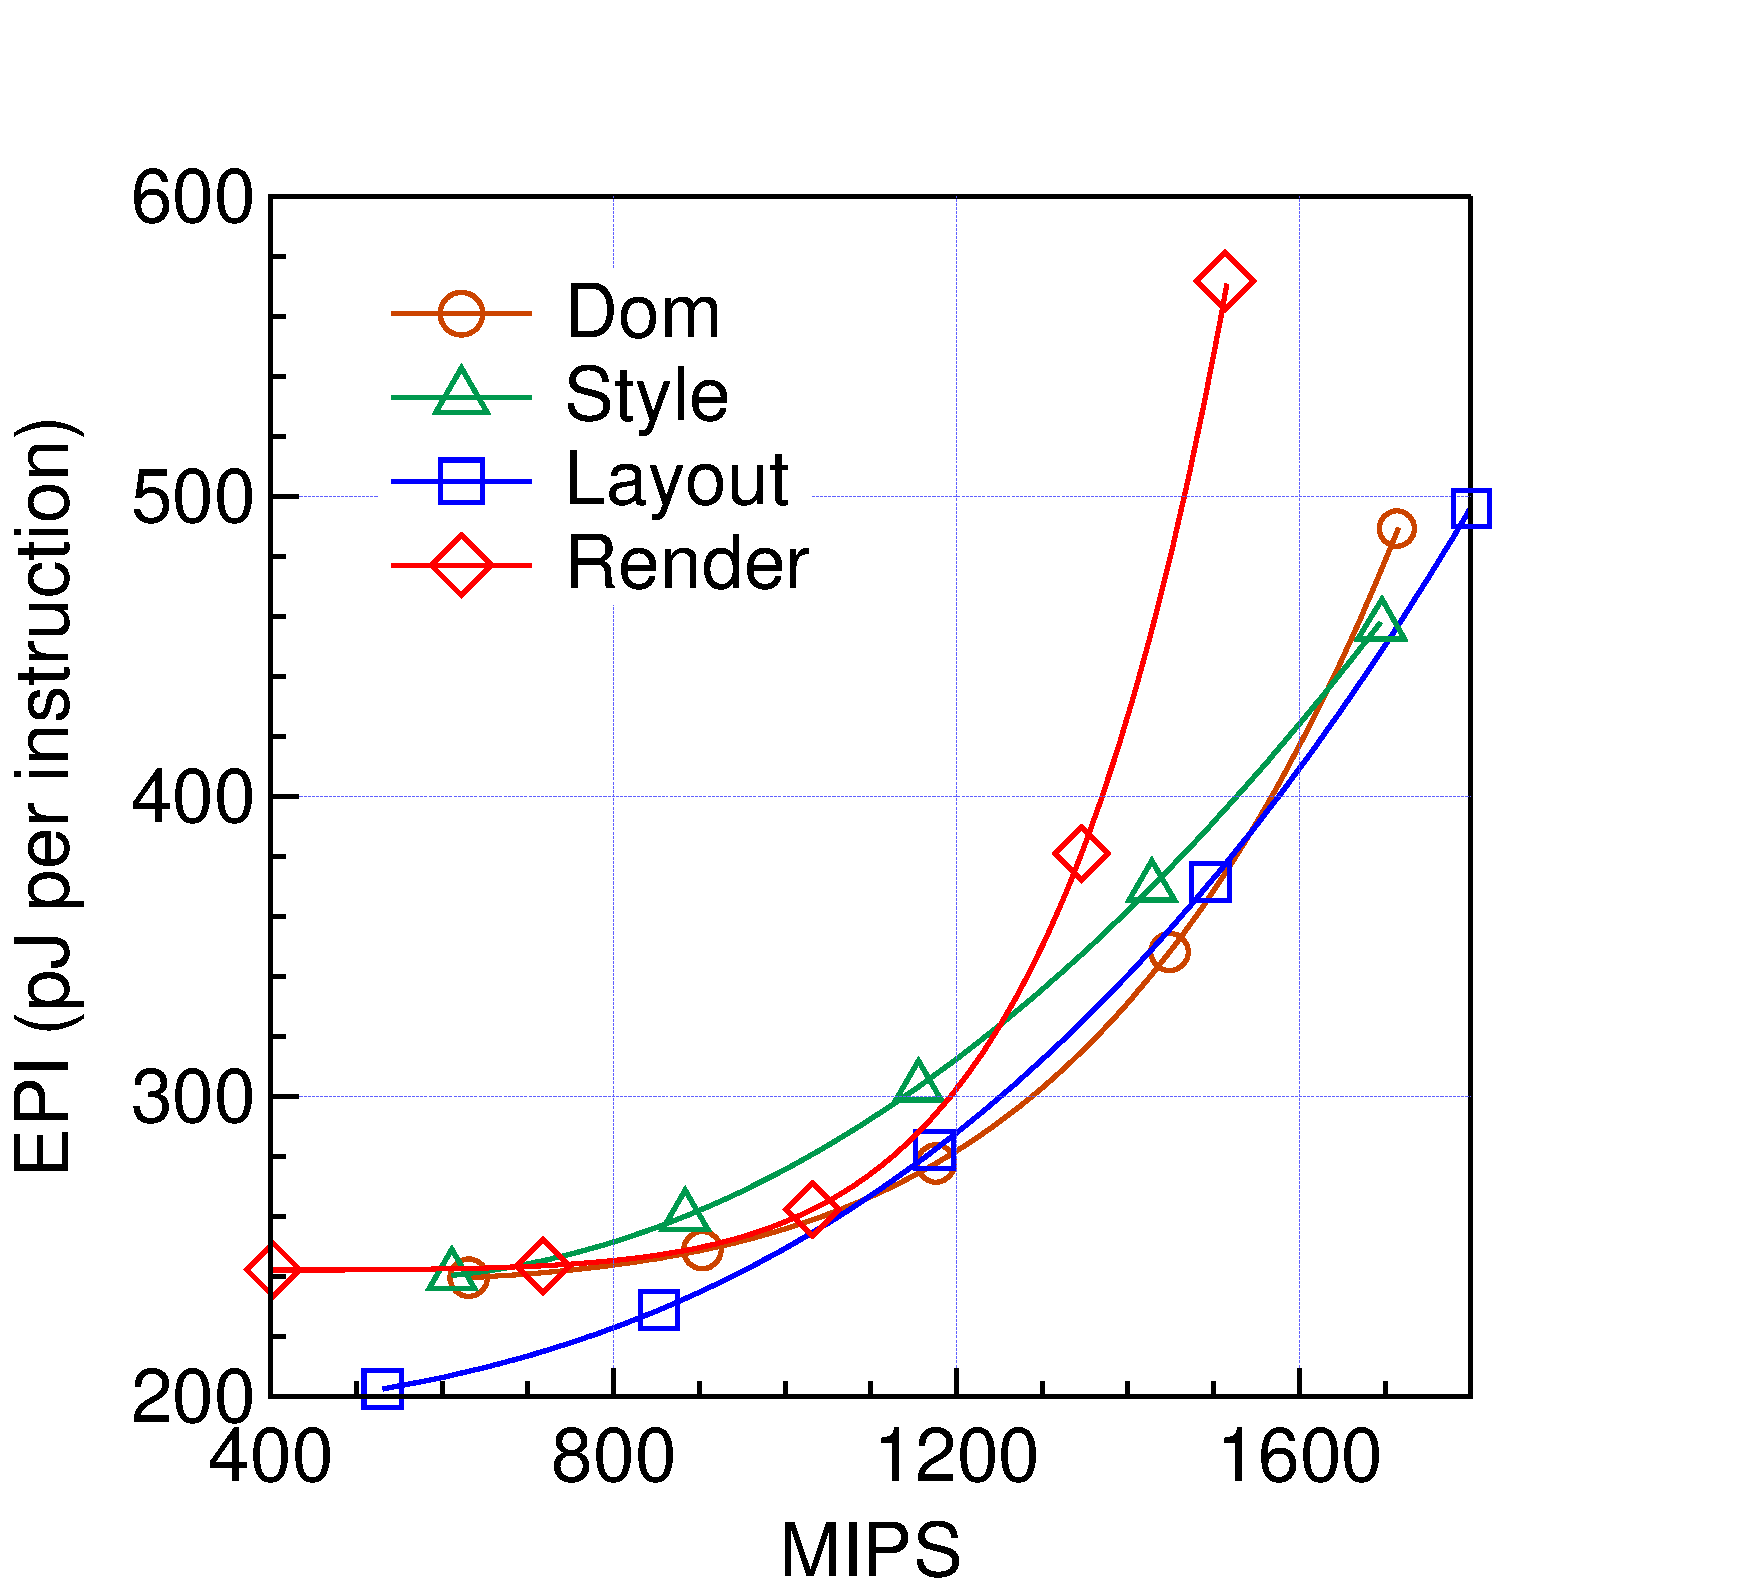
\includegraphics[trim=0 0 0 0, clip, width=.6\columnwidth]{pareto_ooo}
  \caption{Out-of-order Pareto optimal frontier for each kernel.}
  \label{fig:pareto_ooo}
\end{figure}

To understand the difference behind the in-order versus out-of-order designs, we study the kernel behaviors in Web applications. There are four important computation kernels in executing a Web application: i.e.,~\textit{Dom}, \textit{Style}, \textit{Layout}, and \textit{Render}. They contribute to about 75\% of the webpage load time and energy consumption.~\Fig{fig:pareto_io} and~\Fig{fig:pareto_ooo} show the Pareto optimal frontiers of the in-order and out-of-order design space for each kernel. We find that the kernel variance in the in-order designs is more pronounced than in the out-of-order designs. As we push toward more performance in the in-order design space, some kernels stop scaling gracefully on the energy-versus-delay curve, and eventually become a performance bottleneck. Overall, in-order designs have low marginal performance value with high marginal energy cost~\cite{marginal}. In contrast, out-of-order cores can cover the variances across the different kernels through complex execution logic and, therefore, provide wider performance and energy trade-off range.

\subsection{Sources of Inefficiency}
\label{sec:arch:customization:sources}

DSE also helps customization at the microarchitecture level. We examine microarchitectural parameters of two out-of-order Pareto optimal designs: P1 and P2 in \Fig{fig:ivso}. They represent designs optimized for different performance and energy targets. P1 is optimized for minimal energy consumption in the out-of-order space. P2 is a high-performance design with a performance of 1500 MIPS (million instructions per second). \Tbl{tab:dse:ednp} summarizes the microarchitecture configurations of the two designs. For comparison purposes, it also lists the same parameters for ARM Cortex-A15, which represents today's high-end mobile CPU.

%!TEX root=../../paper.tex

\begin{table}[p]
\large
\centering
\captionsetup{width=.9\columnwidth}
\caption{Microarchitecture configurations for P1 and P2 in
\Fig{fig:ivso}. They represent different energy-delay trade-offs. For comparison purpose, we also show the parameters for ARM Cortex-A15, whose information is gather from measurements using the 7-Zip LZMA Benchmark~\cite{7cpu-a15} and ARM's public presentation~\cite{a15-slide}.}
\renewcommand*{\arraystretch}{1.4}
\renewcommand*{\tabcolsep}{15pt}
\resizebox{.9\columnwidth}{!}
{
	\begin{tabular}{l c c c}
	\toprule[0.15em]
        ~      & \bigstrut\textbf{P1} & \bigstrut\textbf{P2} & \bigstrut\textbf{Cortex-A15}\\
	\midrule[0.05em]
        Issue width						&	1		&	3	&	3	\\
        \# Functional units				&	2		&	3	&	8	\\
        Load queue size (\# entries)		&	4		&	16	&	16	\\
        Store queue size (\# entries)	&	4		&	16	&	16	\\
        BTB size (\# entries)   &       1024    &       128 &   64       \\
        ROB size (\# entries)			&	128		&	128	&	40+	\\
        \# Physical registers			&	128		&	128	&	?	\\
        L1 I-cache size (KB)				&	64		&	128	&	32	\\
        L1 I-cache delay (cycles)		&	1		&	2	&	?	\\
        L1 D-cache size (KB)				&	8		&	64	&	32	\\
        L1 D-cache delay (cycles)		&	1		&	1	&	4	\\
        L2 cache size (KB)				&	256&	1024	&	512\textasciitilde4096	\\
        L2 cache delay (cycles)			&	16		&	16	&	21	\\
	\bottomrule[0.15em]
    \end{tabular}
}
\label{tab:dse:ednp}
\end{table}


By comparing P1 and P2 with Cortex-A15, we find two major sources of inefficiencies in general-purpose processors: instruction delivery and data feeding. First, current mobile processors have a small L1 instruction cache that is typically 32~KB in size. However, the two Pareto optimal designs require a 64~KB to 128~KB instruction cache to alleviate the pressure on instruction delivery in mobile Web applications. The pathological front-end behavior mainly stems from the large instruction footprint and the prevalence of the irregular control flow path~\cite{BBench}.

Second, the high-performance design P2 also necessitate a 64~KB data cache, doubling the typical L1 data cache size in current mobile CPUs. The need for a large data cache mainly stems from the large working set size on principal data structures (e.g., the DOM tree) during webpage processing. For example, profiling results show that the average data reuse distance for DOM tree accesses is 4~KB (excluding other memory operations interleaved with DOM accesses). The large data cache leads to excessive energy consumption and needs to be optimized.

\section{Style Resolution Unit}
\label{sec:arch:sru}

Unusual design parameters in a customized processor tuned for the mobile Web workload indicate that instruction delivery and data feeding are critical to guarantee high performance while still being energy efficient. I propose specialized hardware mechanisms to mitigate the instruction delivery and data feeding inefficiencies in the customized out-of-order core designs. In particular, I introduce two new hardware structures: a Style Resolution Unit (SRU) and a Browser Engine Cache (BEC). This section focuses on the SRU and the next section focuses on the BEC.

The SRU is an accelerator for the critical \textit{Style} kernel within the Web browser rendering engine. The SRU design is based on the observation that the \textit{Style} kernel has abundant fine-grained parallelism that is hidden in a software implementation but can be captured by a dedicated hardware structure~(\Sect{sec:sru:motivation}). To exploit the inherent fine-grained parallelism, the SRU employs a multi-lane parallel architecture, which greatly reduces the instruction delivery overhead. To reduce the data feeding pressure, the SRU is tightly coupled with a small scratchpad memory that brings operands closer to the SRU~(\Sect{sec:sru:hw}). To maintain general-purpose programmability, these new hardware structures are accessed via a set of high-level language APIs. The APIs are implemented through a runtime library with only slight modification to the current browser implementation~(\Sect{sec:sru:sw}).

%\Fig{fig:framework} shows an overview of our proposed optimization framework. Overall, the hardware supports fast and energy-efficient execution and data communication, and the library hides the hardware complexity, manages the hardware executions, and eases the software development effort.

\subsection{Motivation}
\label{sec:sru:motivation}

Optimizing the \textit{Style} kernel would improve the overall energy efficiency the most for the following reasons. The~\textit{Style} kernel is the most time-consuming task in the rendering engine. In our profiling, it consumes 35\% of the total rendering engine execution time. it also dominates the energy consumption by consuming 40\% of the total energy.

In order to mitigate the instruction delivery and data communication overhead of the~\textit{Style} kernel, we propose a special functional unit called the~\textit{Style Resolution Unit} (SRU) that is tightly coupled with a small scratchpad memory. The SRU exploits fine-grained parallelism to reduce the amount of instructions and potential divergences. The scratchpad memory reduces data communication pressure by bringing operands closer to the SRU.

\begin{figure}[t]
\centering
\captionsetup{width=\columnwidth}
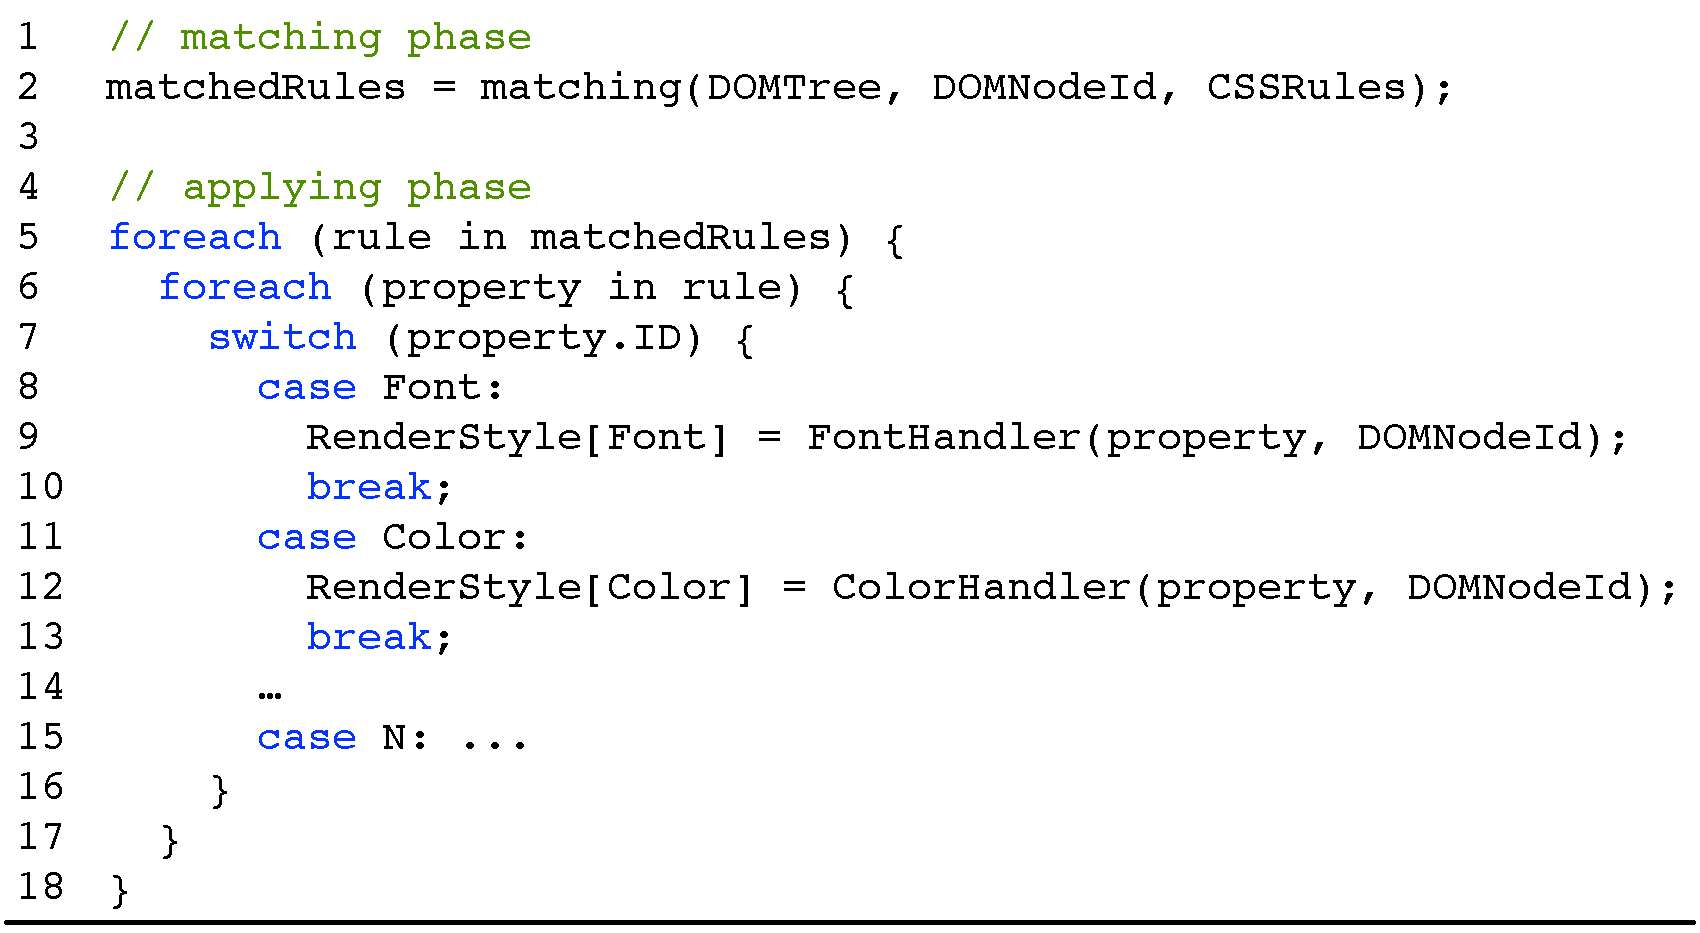
\includegraphics[trim=0 0 0 0, clip, width=\columnwidth]{style-code}
\caption{\small{Pseudo-code of the \textit{Style} kernel. It consists of a matching phase and an applying phase. SRU accelerates the applying phase, which takes about two-thirds of the \textit{Style} kernel execution time.}}
\label{fig:style-code}
\end{figure}

The \textit{Style} kernel consists of two phases: a matching phase and an applying phase. \Fig{fig:style-code} shows the pseudo-code of the two phases. Previous work~\cite{zoomm,ParallelBrowser} focuses on parallelizing the matching phase. However, in our profiling, we find that the applying phase takes nearly twice as long to execute as the matching phase. Therefore, we focus on the applying phase. The applying phase takes in a set of CSS rules (\texttt{matchedRules}) as input, iterates over each rule in the correct cascading order~\cite{cascading} to calculate each style property's final value (e.g., the exact-color RGB values, font width pixels). The final values are stored back to the Render tree (the \texttt{RenderStyle} array).

The key observation we make in the applying phase is that there are two types of inherent parallelism: ``rule-level parallelism'' (RLP) and ``property-level parallelism'' (PLP). Improving the energy efficiency of the~\textit{Style} kernel requires us to exploit both forms of parallelism in order to reduce the control-flow divergence and data communication overheads. Our profiling results indicate that both control flow and memory instructions put together constitute 80\% of the total instructions that are executed within the \textit{Style} kernel.

RLP comes from the following. In order to maintain the correct cascading order, each rule contained in the input data structure must be sequentially iterated from the lowest priority to the highest, so that the higher-priority rules can override the lower-priority rules. However, in reality, we could speculatively apply the rules with different priorities in parallel, and select the one with the highest priority. PLP follows RLP. Each rule has multiple properties, and each property is examined by the engine to set the corresponding data field in the Render tree according to its property ID. Because properties are independent of one another, handling of their processing routines can be dealt with in parallel.

\subsection{Hardware Design}
\label{sec:sru:hw}

We propose a parallel hardware unit that exploits both RLP and PLP, called the Style Resolution Unit. The SRU aggregates enough computations to reduce control-flow divergences and increase arithmetic intensity. It is accompanied by data storage units for both input and output. Note that it is not easy to exploit software-level parallelism for PLP and RLP because of the complex control flow, memory aliasing, and severe loop-carried dependencies.

\begin{figure}[t]
\centering
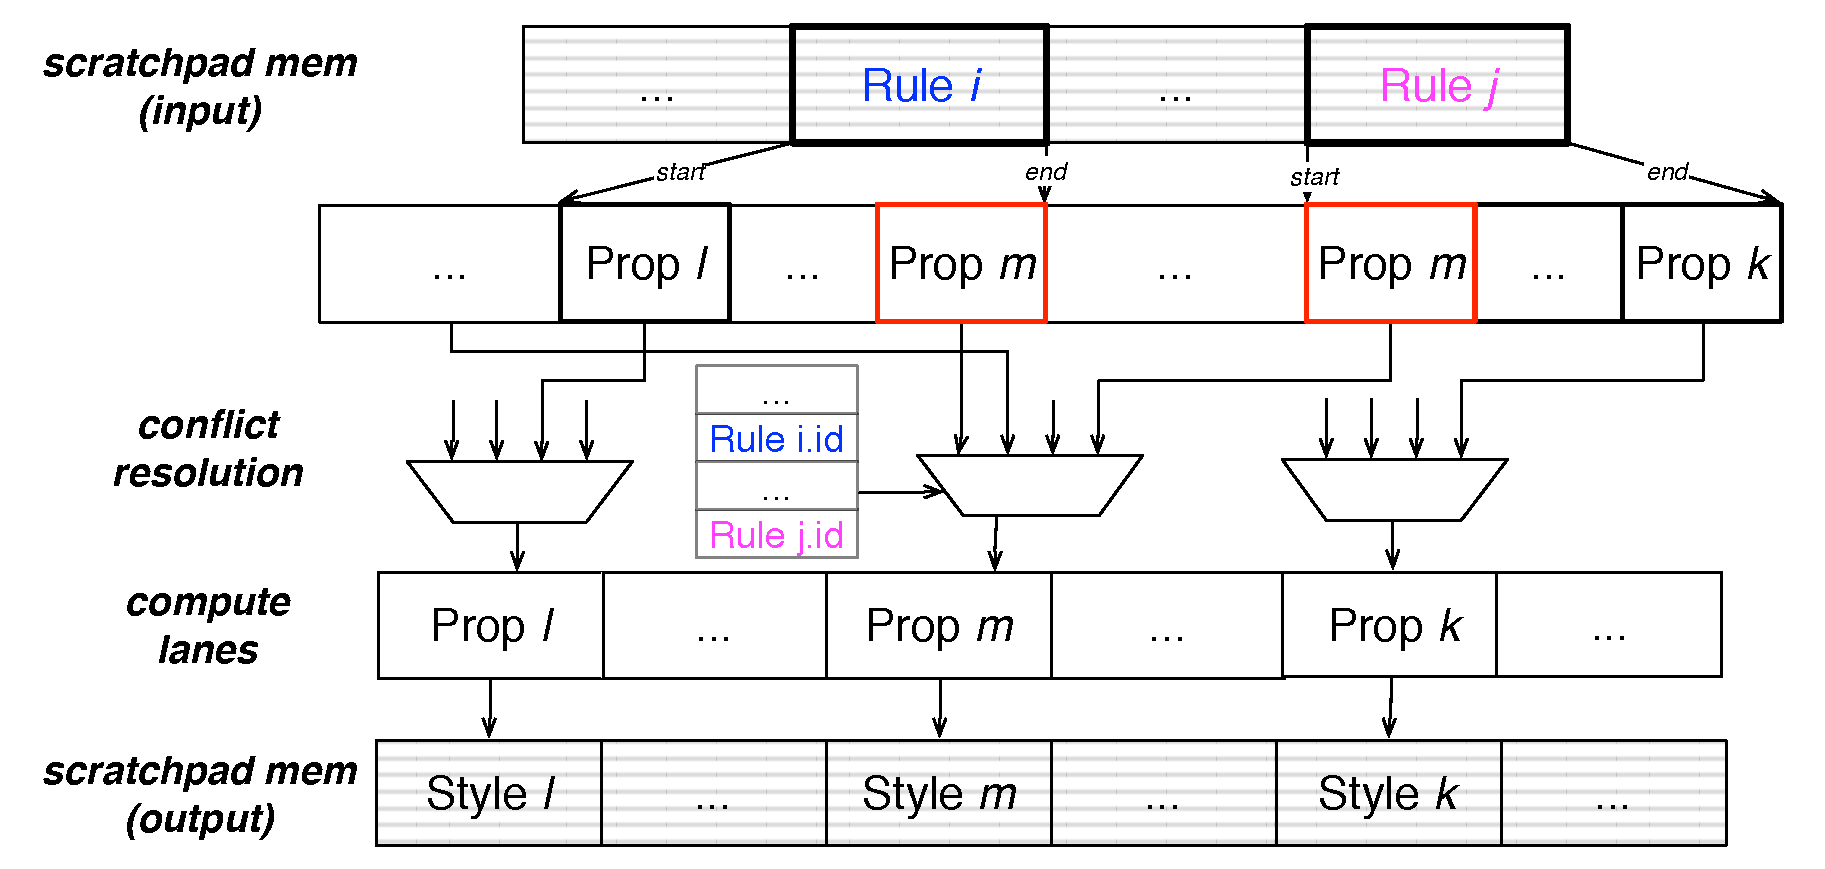
\includegraphics[trim=0 0 0 0, clip, width=\columnwidth]{sru}
\caption{\small{SRU coupled with scratchpad memories.}}
\label{fig:sru}
\end{figure}

In addition, we noticed that the input to the applying phase, \texttt{matchedRules}, is an intra-kernel shared data structure between the matching and applying phases. Storing such short-lived data into the memory hierarchy, and accessing it through traditional load and store instructions, results in slow computation. It also wastes energy. Therefore, we provide a scratchpad memory for the input. Similarly, we store the output structure (i.e., \texttt{RenderStyle}) in a separate scratchpad memory.

\Fig{fig:sru} shows the structure of the SRU with scratchpad memory for input and output data. SRU has multiple lanes, with each lane dealing with one CSS property. Assume Rule~$i$ and Rule~$j$ are two rules from the input that are residing in the scratchpad memory. Rule~$i$ has higher priority than Rule~$j$. Prop~$l$ and Prop~$m$ are two properties in Rule~$i$. Similarly, Rule~$j$ has properties Prop $k$ and Prop $m$. Prop~$l$ and Prop~$k$ can be executed in parallel using different SRU lanes because they do not conflict with each other. However, Prop~$m$ is present in both rules, and as such it causes an SRU lane conflict, in which case the MUX selects the property from the rule with the highest priority, which in our example is Rule~$i$.

%At execution time upon reaching the \texttt{Style\_Apply()} API that programmers use for trigerring the applying phase, the runtime layer copies all the matched rules into the scratchpad memory before the applying phase starts, issue instructions to the SRU, and copies the final style values back to the memory once SRU finishes.

\paragraph{Design Considerations} A hardware implementation can have only a fixed amount of resources. Therefore, the number of SRU lanes and the size of the scratchpad memory is limited. Prior work~\cite{big-little} shows that the number of matched CSS rules and the number of properties in a rule can vary from one webpage to another. As such, a fixed design may overfeed or underfeed the SRU if the resources are not allocated properly.

\begin{figure}[t]
\centering
\subfloat[\small{RLP analysis.}]
{
  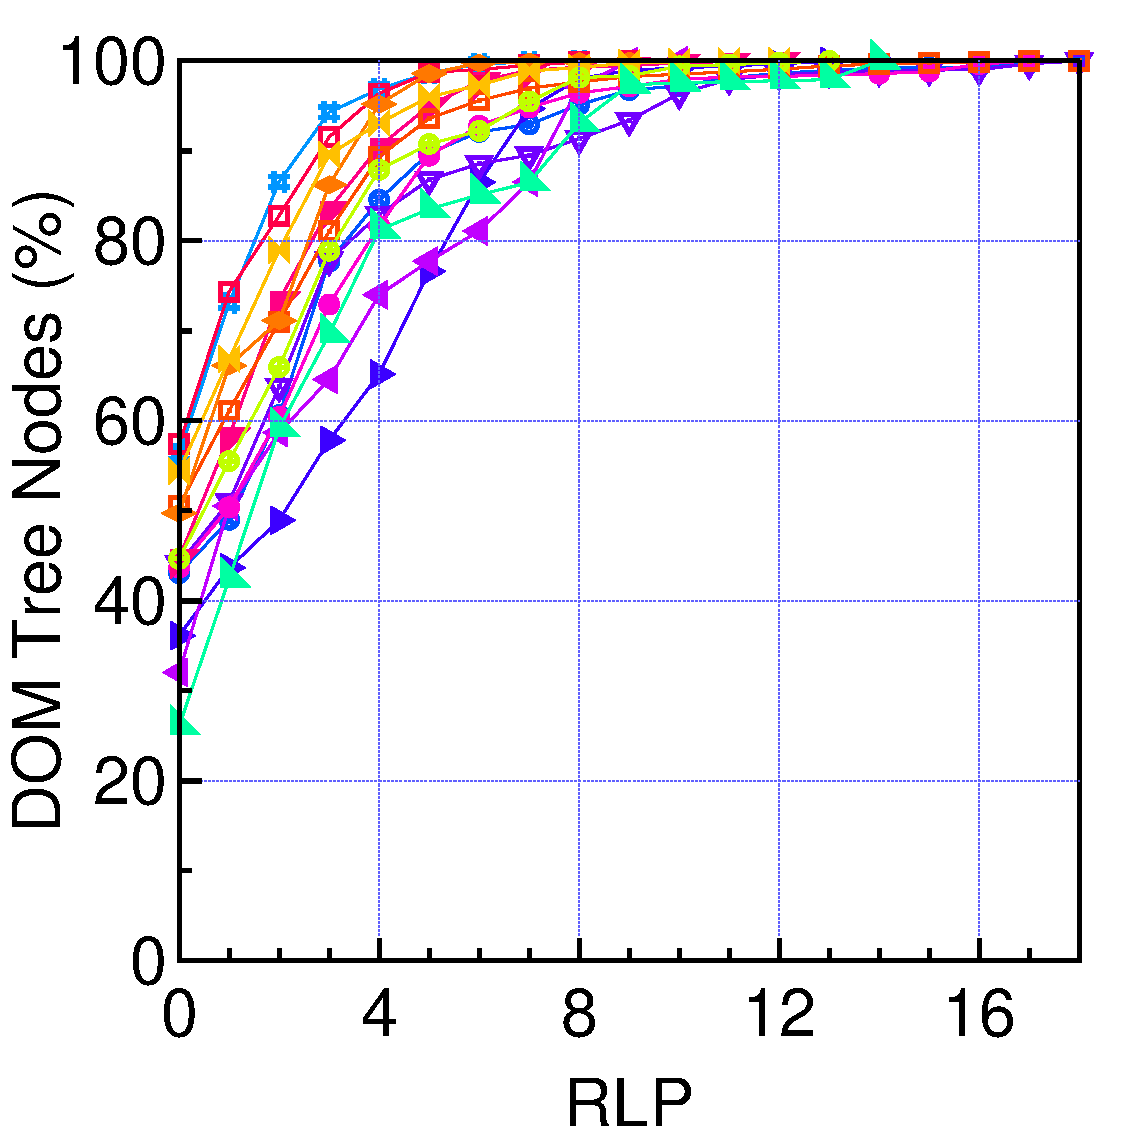
\includegraphics[trim=0 0 0 0, clip, width=.45\columnwidth]{rlp}
  \label{fig:rlp}
}
\hspace*{15pt}
\subfloat[\small{CSS property analysis.}]
{
  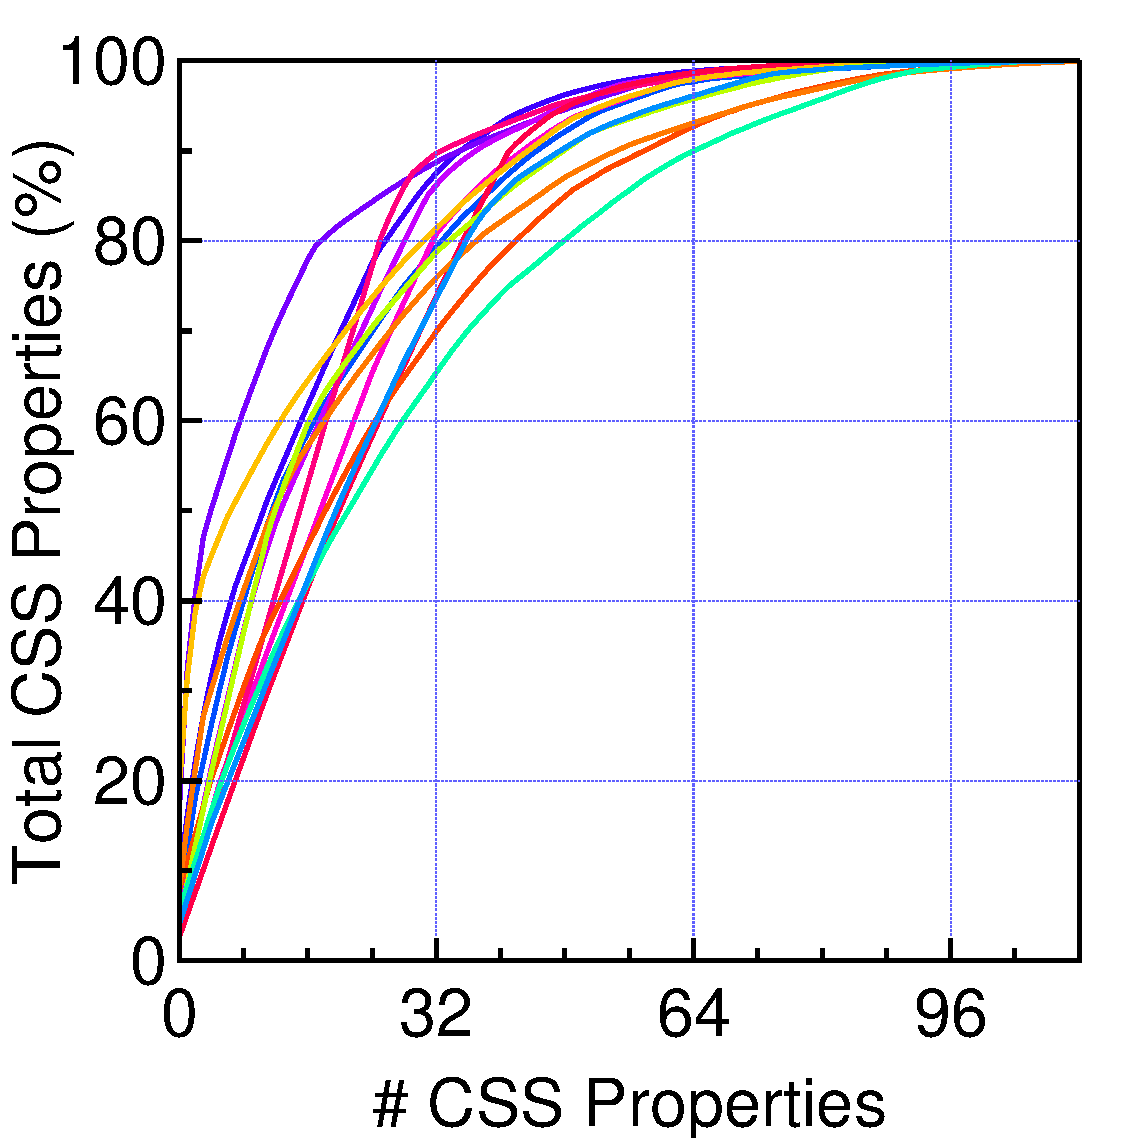
\includegraphics[trim=0 0 0 0, clip, width=.45\columnwidth]{plp}
  \label{fig:plp}
} 
\caption{\small Analysis of RLP and CSS properties across webpages.}
\label{fig:para}
\end{figure}

We profile the webpages to determine the appropriate amount of resource allocation required for the SRU. Profiling indicates that 90\% of the time, the RLP is below or equal to 4 (\Fig{fig:rlp}). Therefore, our design's scratchpad memory only stores up to four styles. Similarly, 32 hot CSS properties cover about 70\% of the commonly used properties (\Fig{fig:plp}). Thus, we implement a 32-wide SRU where each lane handles one hot CSS property. Due to these considerations, the input and output scratchpad memories are each 1~KB in size.

Furthermore, not all of the properties are delegated to the SRU. For example, some style properties require information on the parent and sibling nodes. To avoid complex hardware design for recursions and loops with unknown iterations, we do not implement them in our SRU prototype. The runtime library performs these checks, which we discuss later in~\Sect{sec:sru:sw}. Despite the trade-offs we make, about 72.4\% of the style rules across all the benchmarked webpages can utilize the SRU.  

\subsection{Software Support and Programmability}
\label{sec:sru:sw}

The SRU can be accessed via a small set of instruction extensions to the general-purpose ISA. In order to abstract the low-level details away from application developers, we provide a set of library APIs in high-level languages. Application developers use the APIs without knowing the existence of the specialized hardware. It is important to notice that these software APIs are used by Web browser rendering engine developers rather than high-level Web application developers. WebCore does not affect the programming interface of Web application developers, and therefore has no impact on the Web application development productivity.

\begin{figure}[h]
\centering
\captionsetup{width=.8\columnwidth}
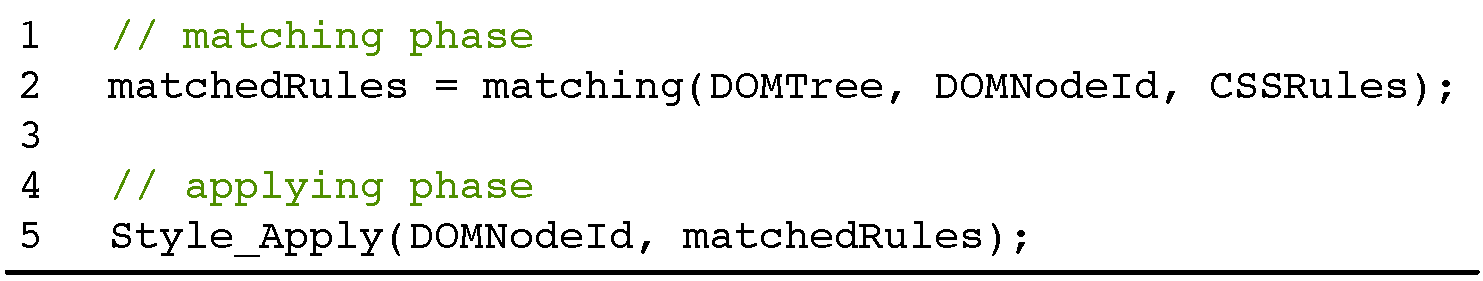
\includegraphics[trim=0 0 0 0, clip, width=.9\columnwidth]{style-code-sru}
\caption{\small{Pseudo-code of the \textit{Style} kernel with the new API.}}
\label{fig:style-code-sru}
\end{figure}

Programmers trigger the style resolution task by issuing a~\texttt{Style\_Apply(Id, Rules)} API, in which \texttt{Id} represents a DOM tree node ID and \texttt{Rules} represents matched CSS rules produced by the matching phase. \Fig{fig:style-code-sru} illustrates the pseudo-code of the \textit{Style} kernel using the provided API. Comparing against the original code in \Fig{fig:style-code}, we notice that the matching phase is not changed while the applying phase is greatly simplified with the \texttt{Style\_Apply} API.

One key task of this API implementation is to examine all the CSS properties of a particular DOM node because not all the CSS properties are implemented in the SRU (as discussed in~\Sect{sec:sru:hw}). For properties that can be offloaded to the SRU, the API implementation loads related data into the SRU's scratchpad memory. For those ``unaccelerated'' properties, the runtime creates the necessary compensation code. Specifically, we propose relying on the existing software implementation as a fail-safe fallback mechanism. Once the style resolution results are generated, the results can be copied out to the output scratchpad memory.

\section{Browser Engine Cache}
\label{sec:arch:cache}

To further improve the energy-efficiency of date feeding, we propose the browser engine cache. It is based on the observation that Web applications' accesses to principal data structures, such as the DOM tree and the Render tree, exhibit heavy data reuse and predictable access pattern~(\Sect{sec:cache:motivation}). Based on such an observation, the browser engine cache uses a small hardware memory structure coupled with a lightweight software-based cache management layer to provide energy-efficient data access~(\Sect{sec:cache:hw}). In addition, similar to SRU, we also provide a set of high-level language APIs that allow Web browser developers to easily access the browser engine cache~(\Sect{sec:cache:sw}).

\subsection{Motivation}
\label{sec:cache:motivation}

\begin{figure}[t]
\centering
\subfloat[\small{DOM node reuse behavior.}]
{
	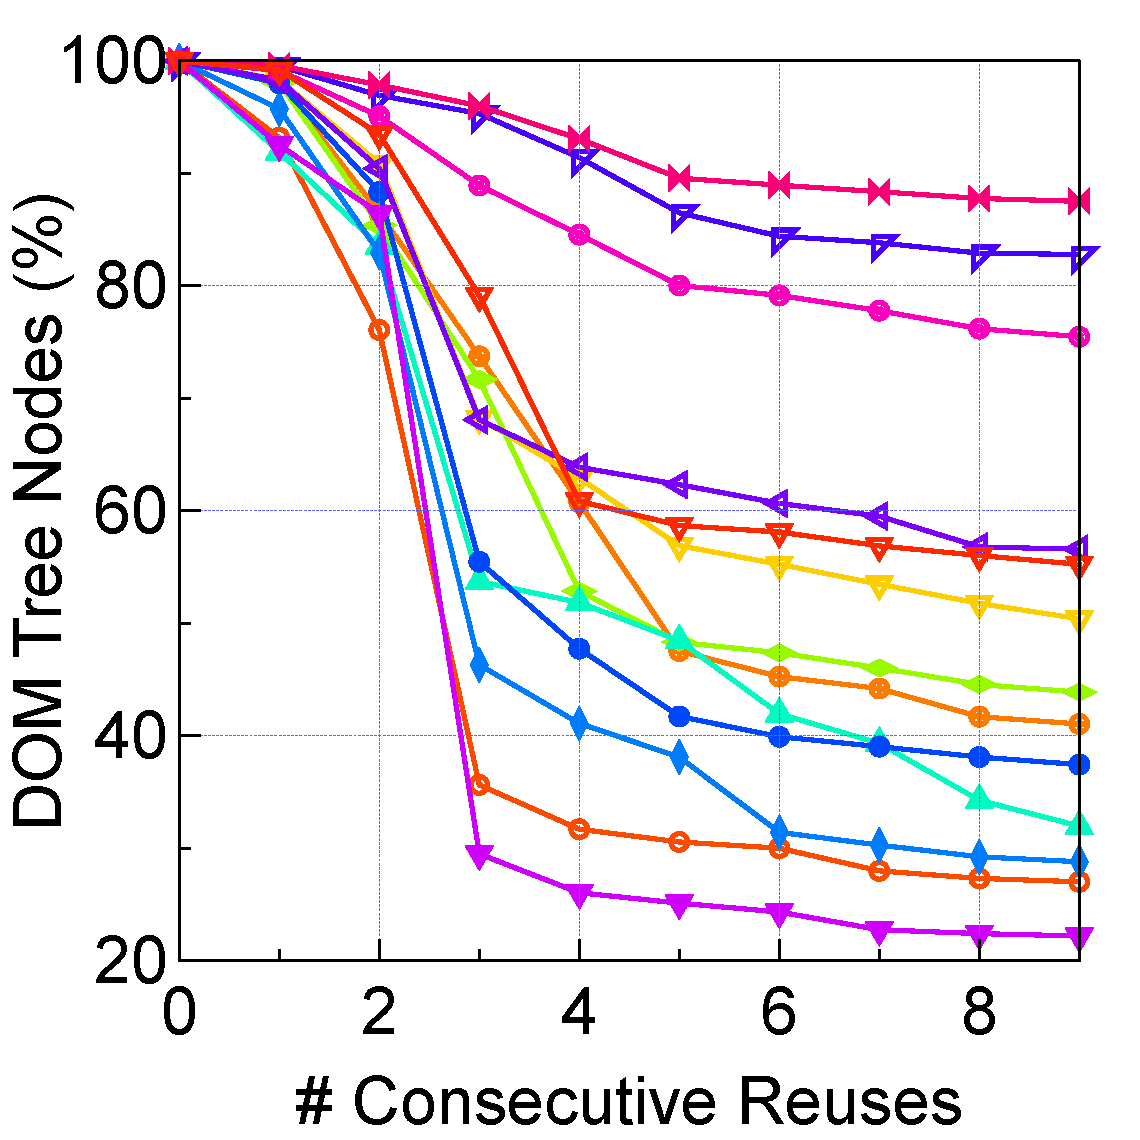
\includegraphics[trim=0 0 0 0, clip, width=.45\columnwidth]{cdf-con-reuse}
	\label{fig:con-reuse}
}
\hspace*{15pt}
\subfloat[\small{DOM node access hit rate.}]
{
	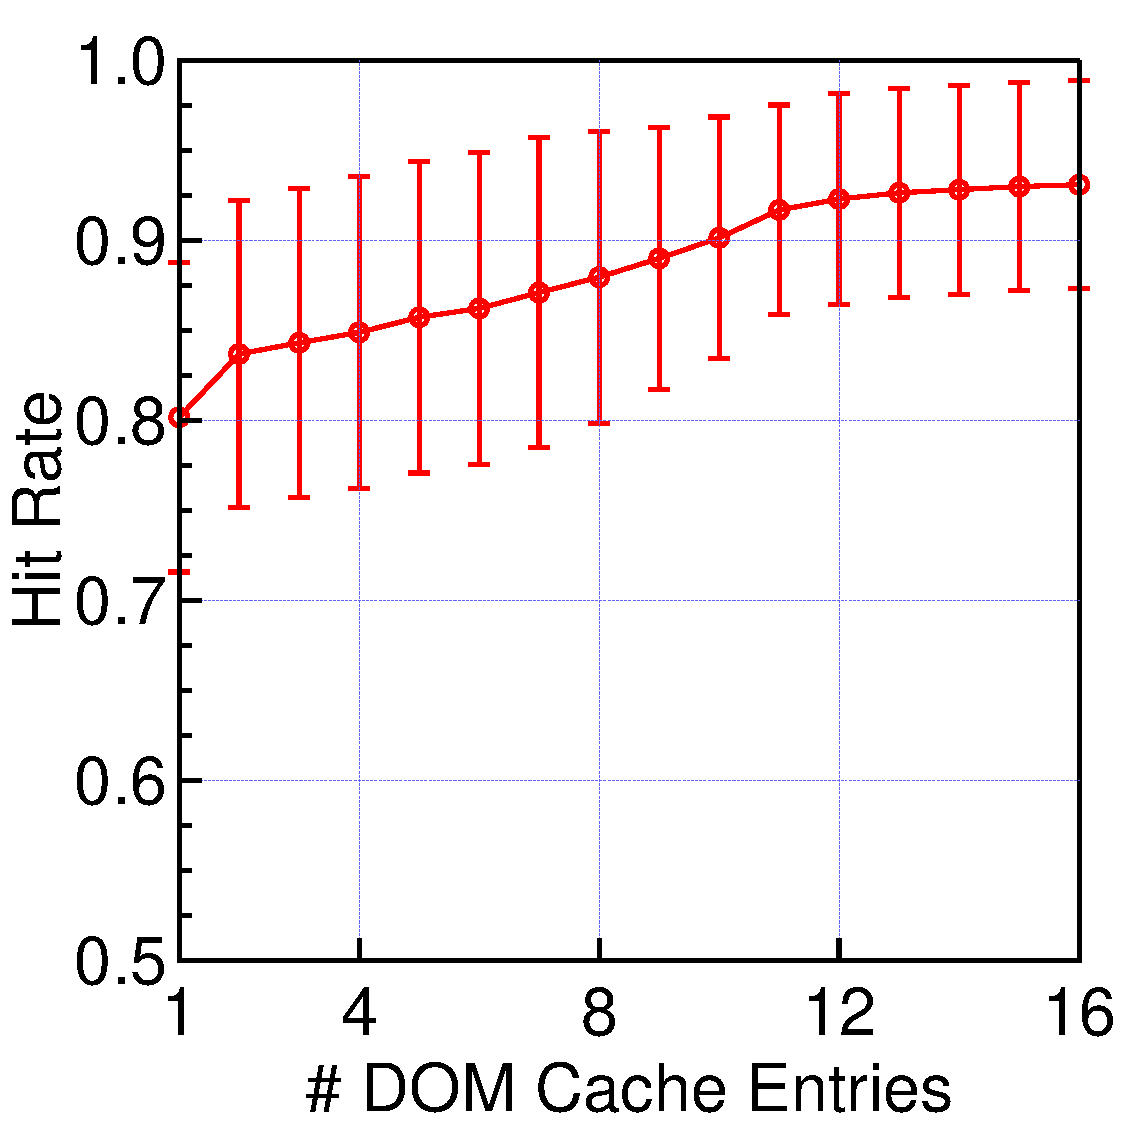
\includegraphics[trim=0 0 0 0, clip, width=.45\columnwidth]{hit-rate}
	\label{fig:hit-rate}
} 
\caption{\small DOM tree access behavior across webpages.}
\label{fig:dom-loc}
\end{figure}

The DOM tree and Render tree are the two most important data structures because they are shared across different kernels. We propose the Browser Engine Cache to improve the energy-efficiency of accessing them. Specifically, the browser engine cache consists of a DOM cache and a Render cache for the DOM tree and Render tree, respectively. We use the DOM to explain our locality observation. Similar analysis and design principles also apply to the render cache. Note that the browser engine cache focuses on improving the energy efficiency of data feeding. We will discuss techniques for improving the performance aspect of data accesses in \Sect{sec:arch:related}.

The energy inefficiency of the traditional cache is best embodied in the performance-oriented design P2 in~\Tbl{tab:dse:ednp}. P2 requires a larger data cache (64~KB) compared to a traditional mobile core. Although a large cache achieves a high hit rate of 93\%, it leads to almost one-fourth of the total energy consumption. However, through careful characterizations, we find that accesses to the DOM/Render tree have strong locality and regular access pattern such that they can benefit from a small and energy-efficient cache memory, rather than the large power-hungry traditional caches. Let us explain our observations below.

First, we find that data accesses to the DOM tree have heavy reuses. \Fig{fig:con-reuse} shows the cumulative distribution of DOM tree node reuse. Each~($x, y$) point corresponds to a portion of DOM tree nodes~($y$) that are consecutively reused at least a certain number of times~($x$). About 90\% of the DOM tree nodes are consecutively reused at least three times, which reflects strong data locality. This indicates that a very small cache can achieve the similar hit rate as a regular cache, but with much lower power.

Second, we find that the accesses to the DOM tree have regular stream-like patterns. To illustrate this,~\Fig{fig:data-acs} shows two representative data access patterns to the DOM tree from \website{www.sina.com} and \website{www.slashdot.org}. Each ($x, y$) point is read as follows. The $x$-th access to the DOM tree operated on the $y$-th DOM node. We observe a common streaming pattern. Such a streaming pattern is due to the intensive DOM tree traversal that is required by many rendering engine kernels. For example, in order to match CSS rules with descendant selectors such as~``\texttt{div p},'' which selects any~\texttt{$<$p$>$} element that is a descendant of~\texttt{$<$div$>$} in the DOM tree, the~\textit{Style} kernel must traverse the DOM tree, one node at a time, to identify the inheritance relation between two nodes. Similarly, the~\textit{Layout} kernel must traverse the Render tree (recursively) to determine the size of each webpage element, which in turn depends on the sizes of the elements contained within it.

In summary, the rendering engine typically operates on one DOM tree node heavily and traverses to the next one. After the rendering engine moves past a DOM node, it is rarely re-referenced soon. Such a unique access behavior motivates the browser engine cache design as we describe below.

\subsection{Hardware Design}
\label{sec:cache:hw}

We propose the DOM cache to capture the DOM tree data locality. It sits between the processor and the L1 cache, effectively behaving as an L0 cache. Each cache line contains the entire data for one DOM tree node, which is 698~bytes in our design. Different from the data array in a regular cache, we implement each cache entry (both in the DOM cache and render cache) as a collection of registers instead of a wide cache line.  Each register holds one attribute of the DOM (Render) tree node, and can be individually accessed through special memory instructions from the software.

The motivations to split each DOM cache line into individually addressable registers are as follows. First, not all the attributes of a node are accessed every time a node is referenced such that pre-loading all the node data from L1 cache to the browser engine cache lead to performance and energy penalty. For example, a Render tree node most often is of either \texttt{RenderBlock} or \texttt{RenderInline} type, each of which involves its own set of attributes. The browser can decide what attributes to load depending on what type a Render tree node is. Second, splitting the large memory array into small registers also allows fast and more energy-conserving accesses.

We choose to implement the DOM cache as a ``software-managed'' cache--i.e., the data is physically stored in hardware memory, and the software performs the actual cache management, such as insertion and replacement. Prior work has demonstrated effective software-managed cache implementations~\cite{Hallnor:2000:FAS:339647.339660}. It is possible to implement the DOM cache entirely in hardware, similar to a normal data cache. Our motivation for a software-managed cache is to avoid the complexity of a hardware cache. Typically, the cache involves hardware circuitry whose overhead can be high, especially for extremely small cache sizes.

\begin{figure}[t]
\centering
\subfloat[\small{\website{www.sina.com.cn}}]
{
	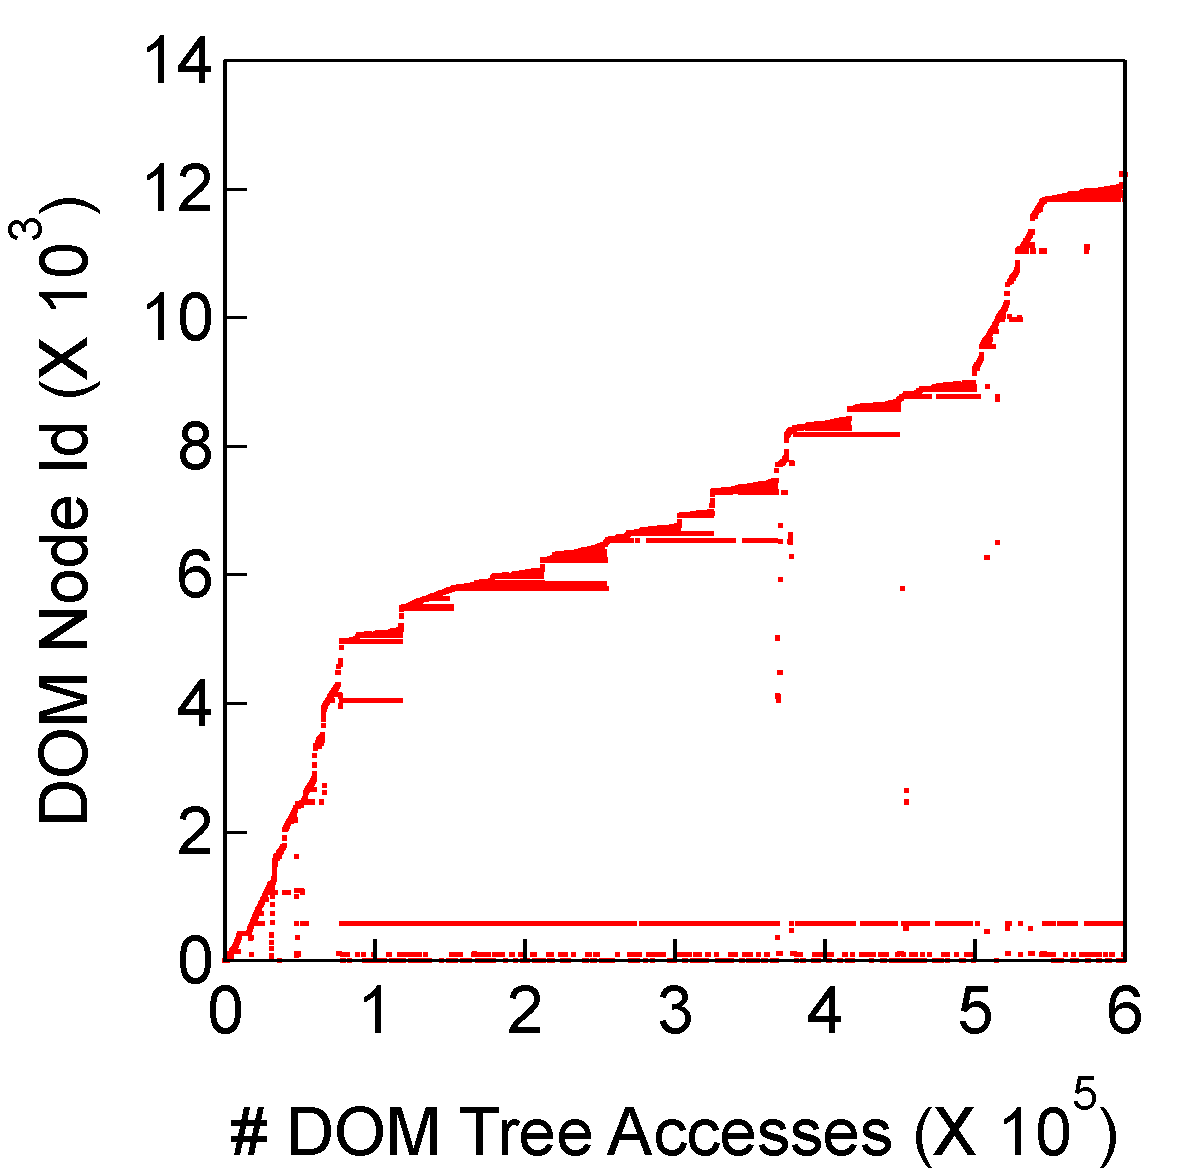
\includegraphics[trim=0 0 0 0, clip, width=.45\columnwidth]{sina}
	\label{fig:sina}
}
\hspace*{15pt}
\subfloat[\small{\website{www.slashdot.org}}]
{
	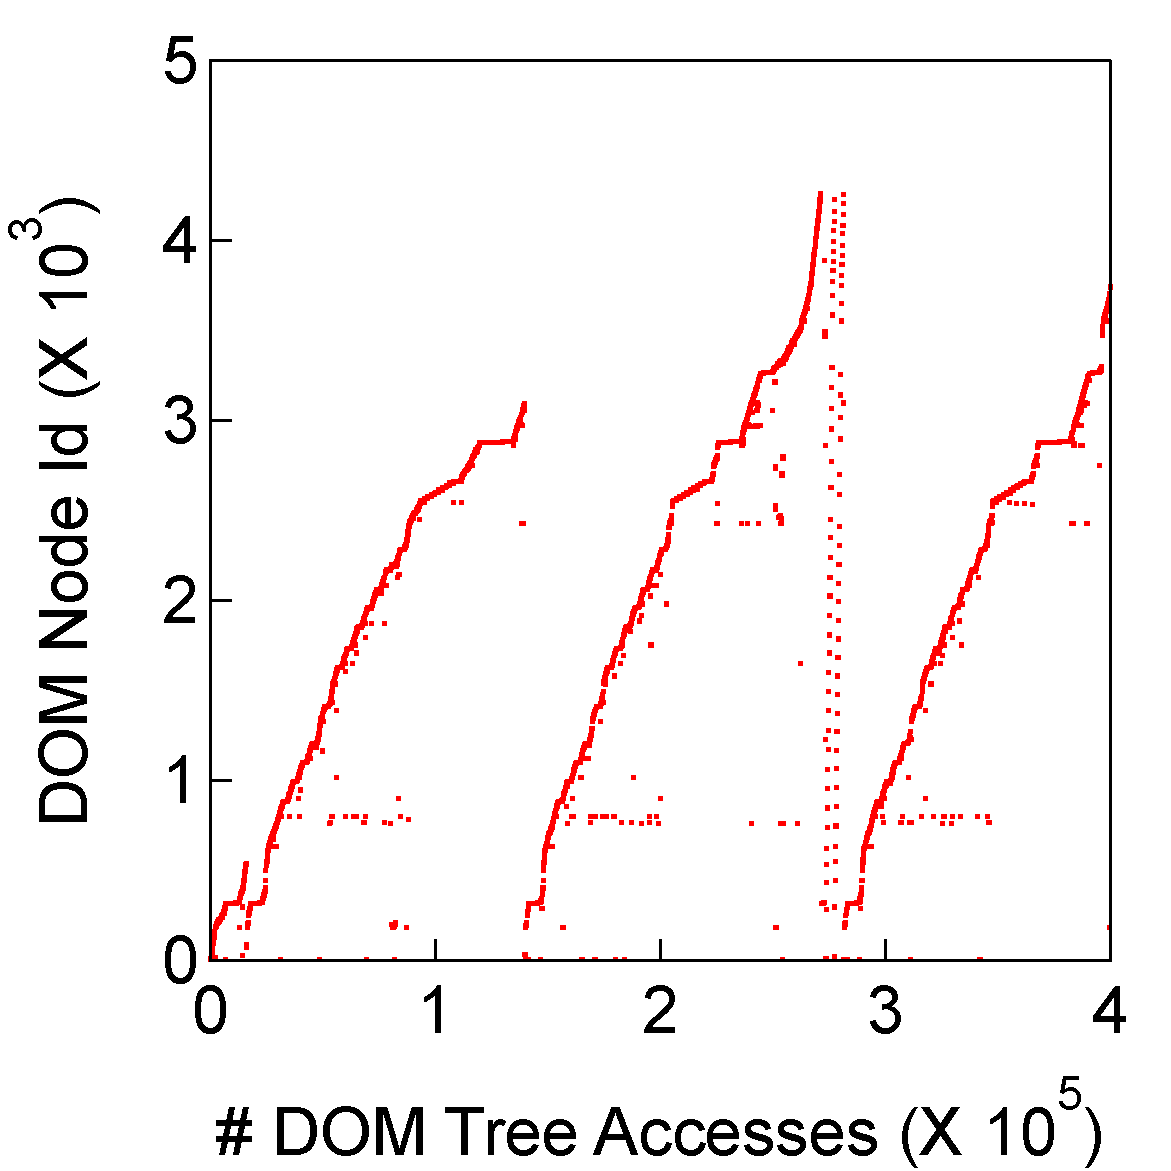
\includegraphics[trim=0 0 0 0, clip, width=.45\columnwidth]{slashdot}
	\label{fig:slashdot}
} 
\caption{\small Representative DOM tree access patterns.}
\label{fig:data-acs}
\end{figure}

The software overhead for the software-managed browser cache is relatively insignificant for the following reasons. First, a simple replacement policy that always evicts the earliest inserted line is sufficient. Due to the streaming pattern shown in~\Fig{fig:data-acs}, DOM tree nodes are rarely re-referenced soon after the browser engine moves past them. Therefore, a simple FIFO design is almost as effective as the least recently used policy, but with much less management overhead.

Second, a very small number of DOM cache entries guarantee a high hit rate. Therefore, the cache-hit lookup overhead is minimal.~\Fig{fig:hit-rate} shows how the hit rate changes with the number of entries allocated for the DOM tree. The curve represents the average hit rate, and the error bars represent the standard deviations across different webpages. Across all the webpages, a 4-entry design can achieve about 85\% hit rate, and so we use this configuration. In this sense, the DOM cache is effectively a single set, 4-way fully associative cache. Similarly, the render cache contains two entries (i.e., two cache lines). On average, it achieves over 90\% hit rate.

\subsection{Software Support and Programmability}
\label{sec:cache:sw}

To access a particular DOM tree node in the rendering engine, developers issue~\texttt{DOMCache\_LD(Id, attr)} and~\texttt{DOMCache\_ST(Id, attr, data)} for read and write operation, respectively. Similar APIs are also provided for the Render Cache. In the provided APIs, \texttt{Id} represents the DOM tree node ID (similar to the \texttt{Style\_Apply()} API), \texttt{attr} represents a particular DOM node attribute, and \texttt{data} indicates the new data of the specified \texttt{attr}. Recall that our DOM cache design allows each attribute of a DOM node to be individually addressed~(\Sect{sec:cache:hw}). The syntax of both APIs allow developers to fully utilize this feature.

\begin{figure}[b]
\centering
\captionsetup{width=\columnwidth}
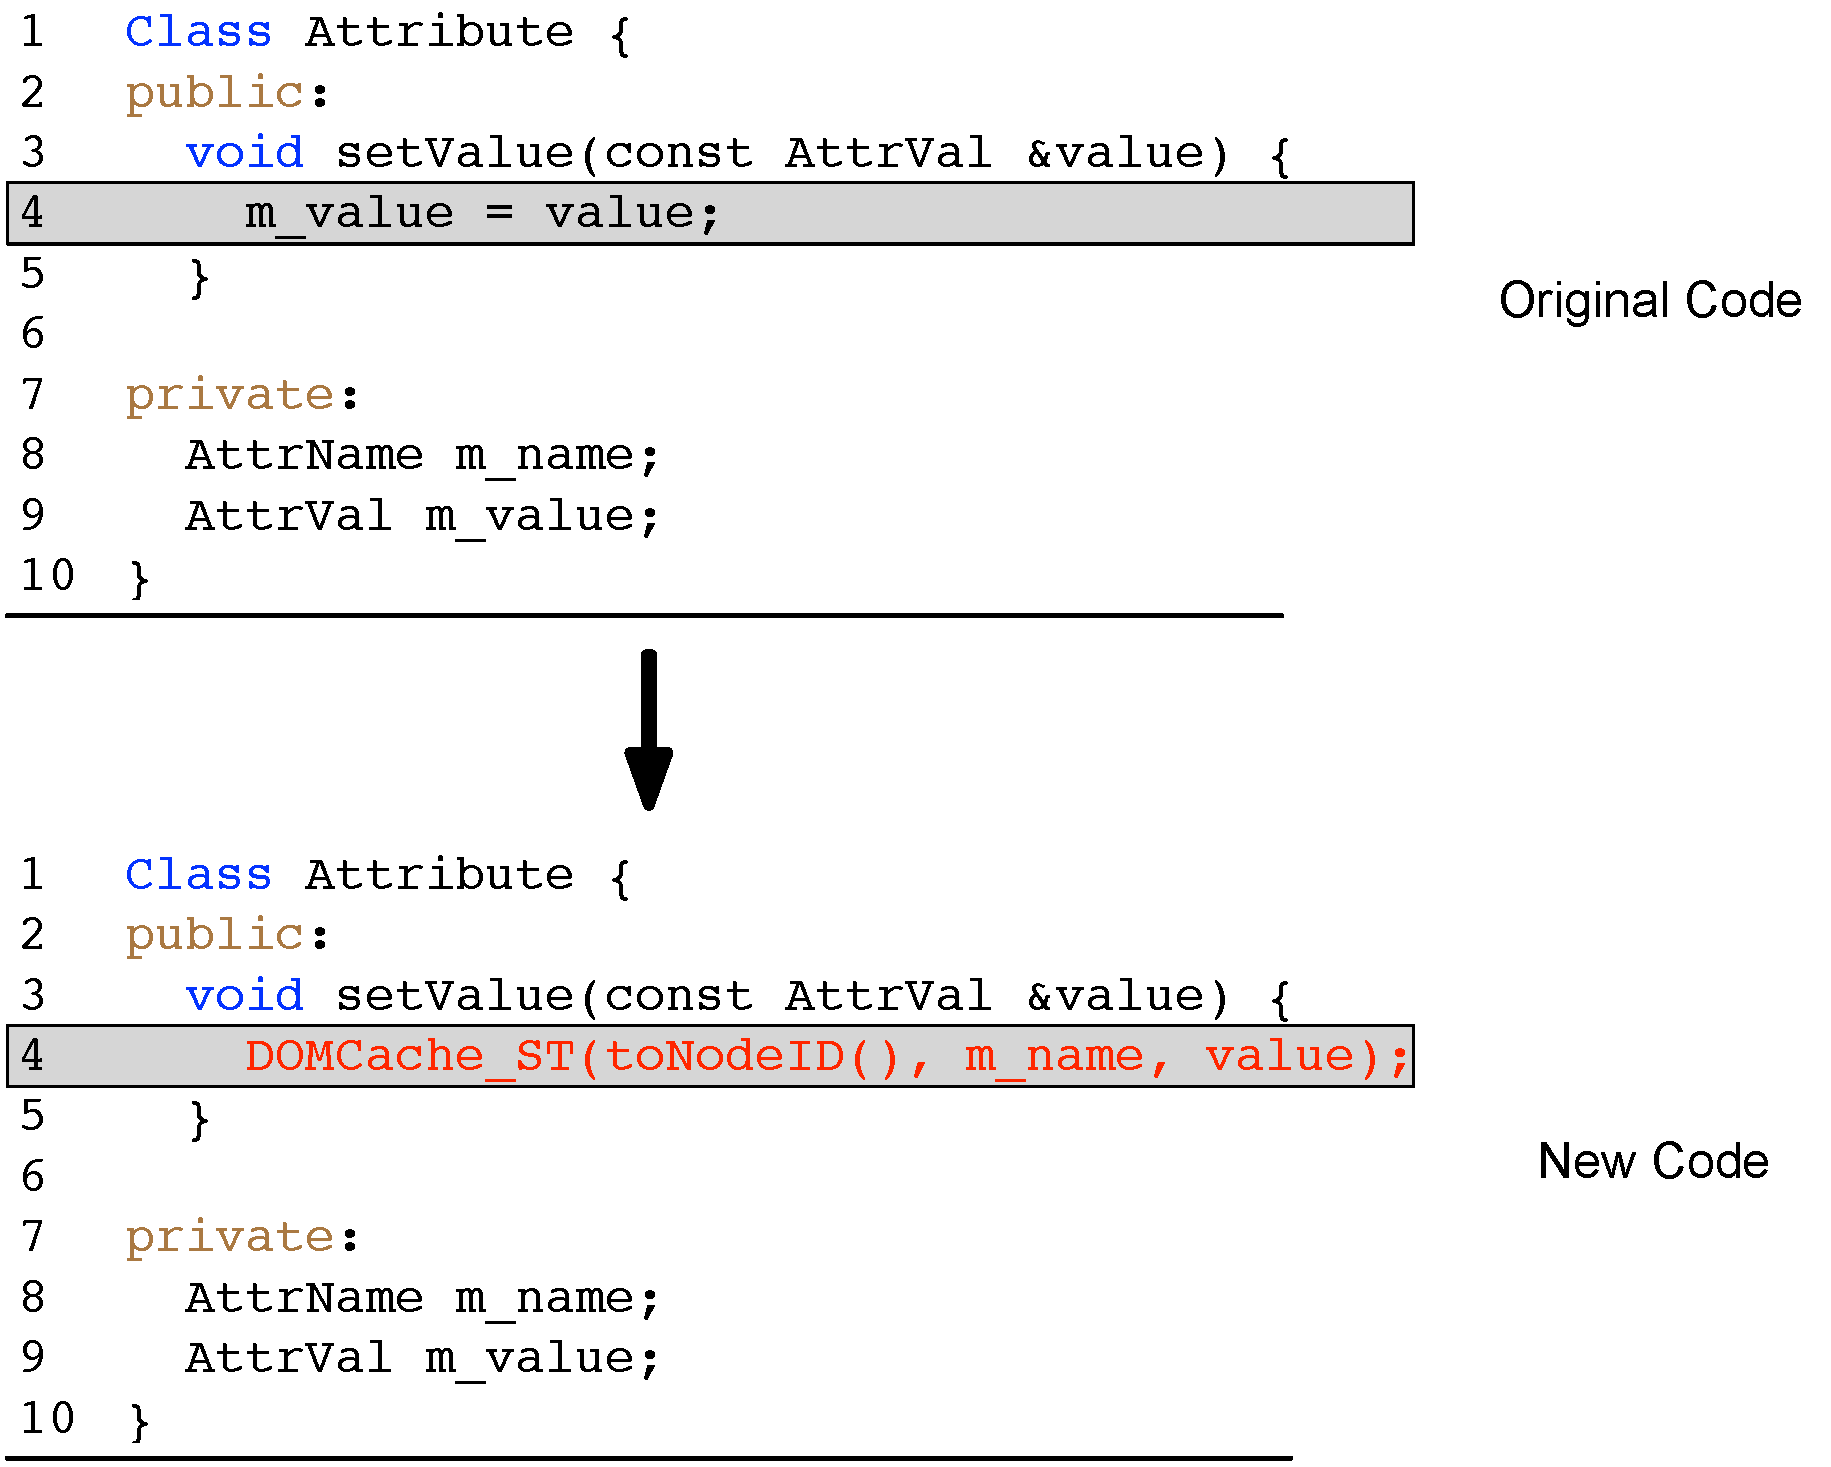
\includegraphics[trim=0 0 0 0, clip, width=\columnwidth]{style-code-cache}
\caption{\small{Using the \texttt{DOMCache\_ST()} API in the rendering engine. The new DOM attribute store API replaces the original attribute value assignment, and performs cache manegement.}}
\label{fig:style-code-cache}
\end{figure}

\Fig{fig:style-code-cache} shows how \texttt{DOMCache\_ST()} API is used in the rendering engine. It is used to set value of any given attribute in the \texttt{setValue()} method of the \texttt{Attribute} class. Specifically, \texttt{DOMCache\_ST()} replaces the original value assignment. The API implementation performs the actual hardware memory accesses as well as cache management, such as replacement and insertion. For example, the API needs to maintain an array, similar to the tag array in a regular cache, to keep track of which DOM nodes are in the cache and whether they are modified.  Effectively, the runtime library of DOM cache APIs implements a cache simulator. However, the runtime overhead is negligible due to the simple cache design as described in~\Sect{sec:cache:hw}.

It is worth noting that using DOM cache APIs only affects the primitive classes of a rendering engine (such as the \texttt{Attribute} class in \Fig{fig:style-code-cache}) while maintaining the interface between primitive classes and the rest of the rendering engine unchanged. For example, rendering engine developers can still use the same \texttt{setValue()} method to update an attribute's value. Therefore, we do not expect using the new APIs to affect the development productivity.

\section{WebCore Evaluation}
\label{sec:arch:eval}

In this section, we first present the power and timing overhead analysis of the proposed specialization techniques~(\Sect{sec:arch:eval:oh}). We then evaluate the energy-efficiency implications of the SRU and the browser engine cache individually~(\Sect{sec:arch:eval:sru}, \Sect{sec:arch:eval:cache}). In the end, we show the energy-efficiency improvement combining both customization and specialization~(\Sect{sec:arch:eval:comb}). In particular, we show that our specializations can achieve significantly better energy efficiency than simply dedicating the same amount of area and power overhead to tune the conventional general-purpose cores.

We evaluate our optimizations against three designs, D1 through D3. D1 refers to the energy-conscious design (P1) that we explored in~\Fig{fig:ivso}. Similarly, D2 refers to the performance-oriented design (P2) in~\Fig{fig:ivso}. D3 mimics the common design configuration of current out-of-order mobile processors. We configure D3 as a three-issue out-of-order core with 32-entry load queue and store queue, 40 ROB entries, and 140 physical registers. It has a 32~KB, 1-cycle latency L1 data and instruction cache, and a 1~MB, 16-cycle latency L2 cache.

\subsection{Overhead Analysis}
\label{sec:arch:eval:oh}

We use CACTI v5.3~\cite{cacti} to estimate the memory structures overhead. We implement the SRU in Verilog and synthesize our design in 28~nm technology using the Synposys toolchain.

\paragraph{Area} The size of SRU's scratchpad memory is 1~KB. The DOM cache size is 2,792~bytes. The render cache size is 1,036~bytes. The hardware requirements for the SRU are mainly comparators and MUXes to deal with control flow, and simple adders with constants inputs to compute each CSS property's final value. In total, the area overhead of the memory structures and the SRU logic is about 0.59~mm\textsuperscript{2}, which is negligible compared to typical mobile SoC size (e.g., Samsung's Exynos 5410 SoC has a total die area size of 122~mm\textsuperscript{2}~\cite{exynox5410diesize}).

\paragraph{Power} The synthesis reports that the SRU logic introduces 70~mW total power under typical stimuli. The browser engine cache and the SRU scratchpad memory add 7.2~mW and 2.4~mW to the dynamic power, respectively. They are insignificant compared to power consumption for Web browsing (in our measurements, a single core Cortex-A15 consumes about 1~W for webpage loading). Clocking gating can reduce the power consumption further~\cite{queuethermal}. But we are conservative in our analysis and do not assume such optimistic benefits.

\paragraph{Timing} Both the browser engine cache and SRU scratchpad memory can be accessed in one cycle, which is the same as the fastest L1 cache latency in our design space. The synthesis tool reports that the SRU logic latency is about 16 cycles under 1.6~GHz. Later in our performance evaluation, we conservatively assume the SRU logic is not pipelined.

\paragraph{Software} The software overhead mainly includes cache management and SRU compensation code creation. The overhead varies depending on individual webpage runtime behaviors. We model these overheads in our performance evaluation and discuss their impact along with the improvements.

\subsection{Style Resolution Unit}
\label{sec:arch:eval:sru}

\begin{figure}[t]
\centering
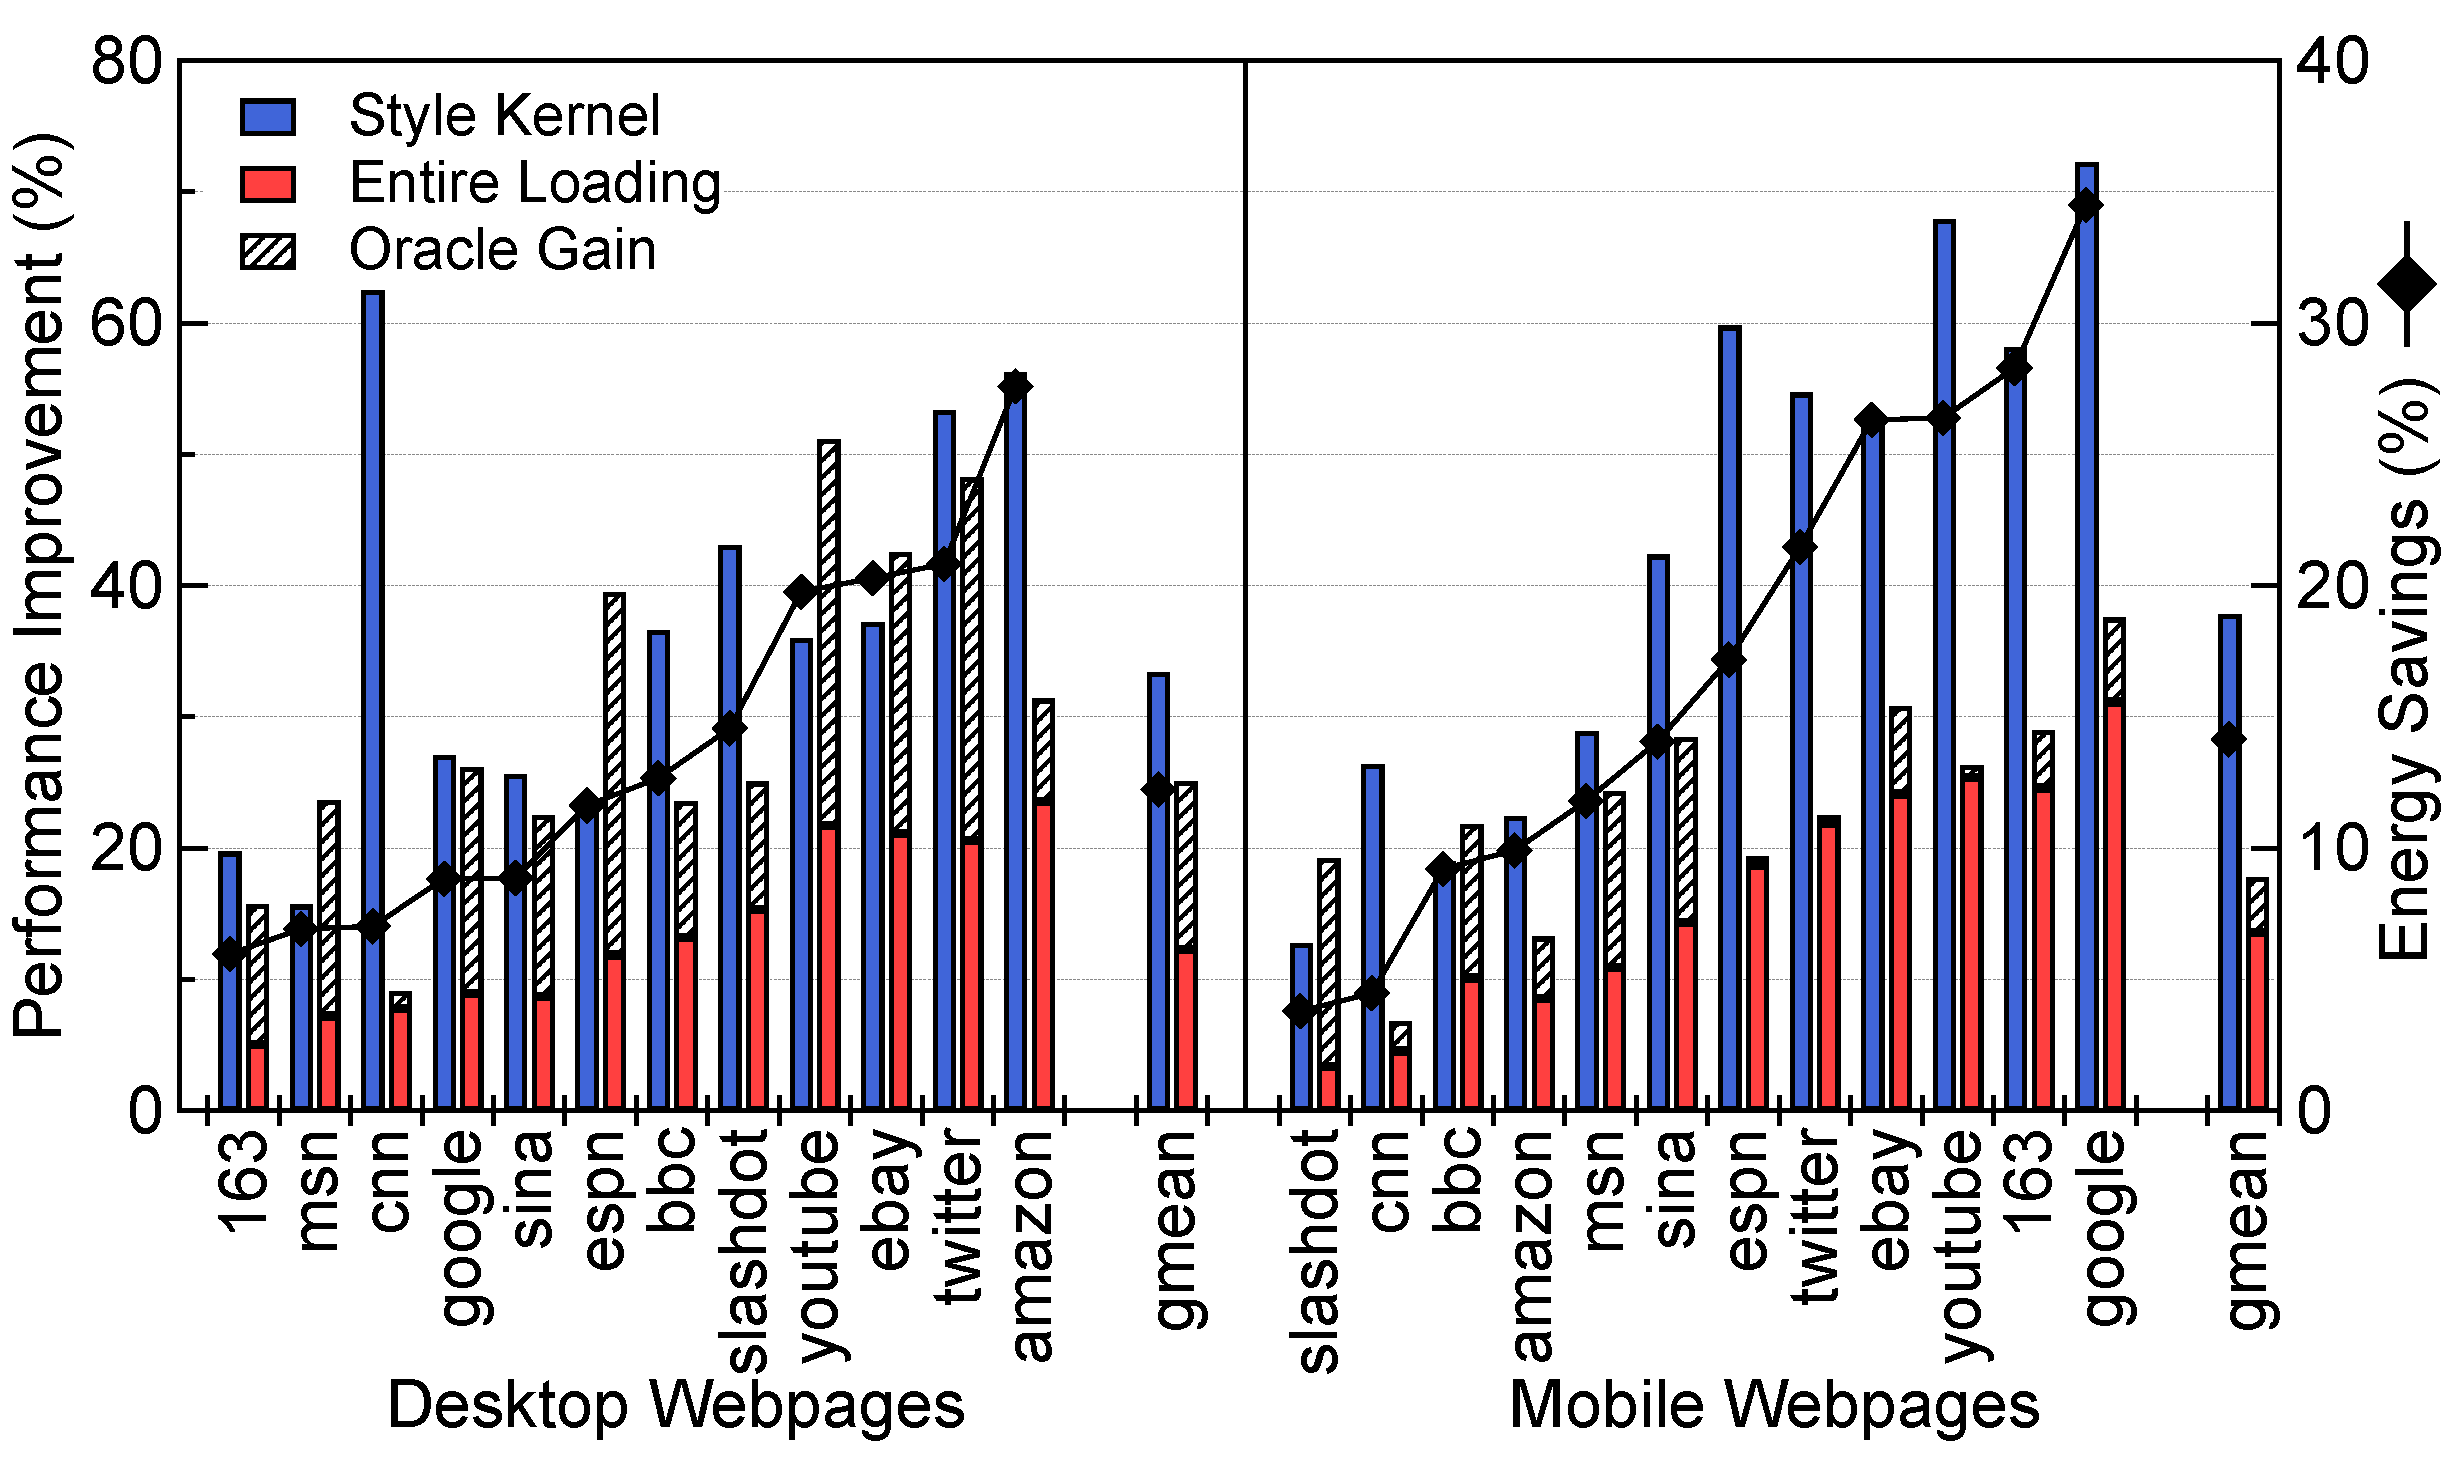
\includegraphics[trim=0 0 0 0, clip, width=\columnwidth]{sru-perf}
\caption{\small{Performance and energy improvement of the SRU.}}
\label{fig:sru-perf}
\end{figure}

Our SRU prototype design achieves on average 3.5X, and up to 10X, speedup for the accelerated style applying phase. The improvements vary because of individual webpage characteristics.

\Fig{fig:sru-perf} shows SRU's performance improvement for the~\textit{Style} kernel and the entire webpage loading on the performance-oriented design D2 in \Fig{fig:ivso}.  The average performance improvement of the~\textit{Style} kernel is 33.4\% and 37.8\% for desktop and mobile webpages, respectively. Generally, we find that mobile webpages benefit slightly more from the SRU because they tend to be less diversified in webpage styling, and therefore the SRU has higher coverage.

The overall improvements vary across webpages because different webpages spend different portions of time in the~\textit{Style} kernel. For example, \website{cnn} spends only 14\% of its execution time in the~\textit{Style} kernel during the entire run. Therefore, its 62\% improvement in the~\textit{Style} kernel translates to an overall improvement of only 7\%. On average, the SRU improves the entire webpage load time by 13.1\% on all the webpages.

The SRU not only improves performance but also reduces energy consumption. The right $y$-axis of~\Fig{fig:sru-perf} shows the energy saving for the entire webpage loading. Webpages are sorted according to the energy savings. On average, SRU results in 13.4\% energy saving for all webpages.

\Fig{fig:sru-perf} also shows the oracle improvement if the entire applying phase can be delegated to the SRU (i.e., no hardware resource constraints). Desktop webpages have much higher oracle gain than mobile webpages. The software fall-back mechanism is more frequently triggered in desktop-version webpages due to their diversity in styling webpages. This also implies the potential benefits of reconfiguring the SRU according to different webpages. An SRU that is customized for mobile webpages could potentially be much smaller.

We apply the SRU to different designs to show its general applicability. For loading an entire webpage, on a current mobile processor design (D3), the SRU improves performance by 10.0\% and reduces energy consumption by 10.3\%. On an energy-conscious design (D1), it improves performance by 8.4\% and reduces energy consumption by 11.6\%.

\subsection{Browser Engine Cache}
\label{sec:arch:eval:cache}

\Fig{fig:cache-energy} shows the energy reduction from using the browser engine cache. The browser engine cache can serve data more energy-efficiently because of the high hit rate of its cache (as shown in~\Fig{fig:hit-rate}). Mobile webpages achieve less energy saving than desktop-version webpages because of their smaller memory footprint. On average, the performance-oriented design (D2) achieves 14.4\% energy savings. Since the energy-conscious (D1) and current design (D3) have smaller caches, the energy consumption caused by the data cache is less, and therefore benefits less from the browser engine cache. On average, their energy consumption reduces by 5.9\% and 9.3\%, respectively.

\begin{figure}[t]
\centering
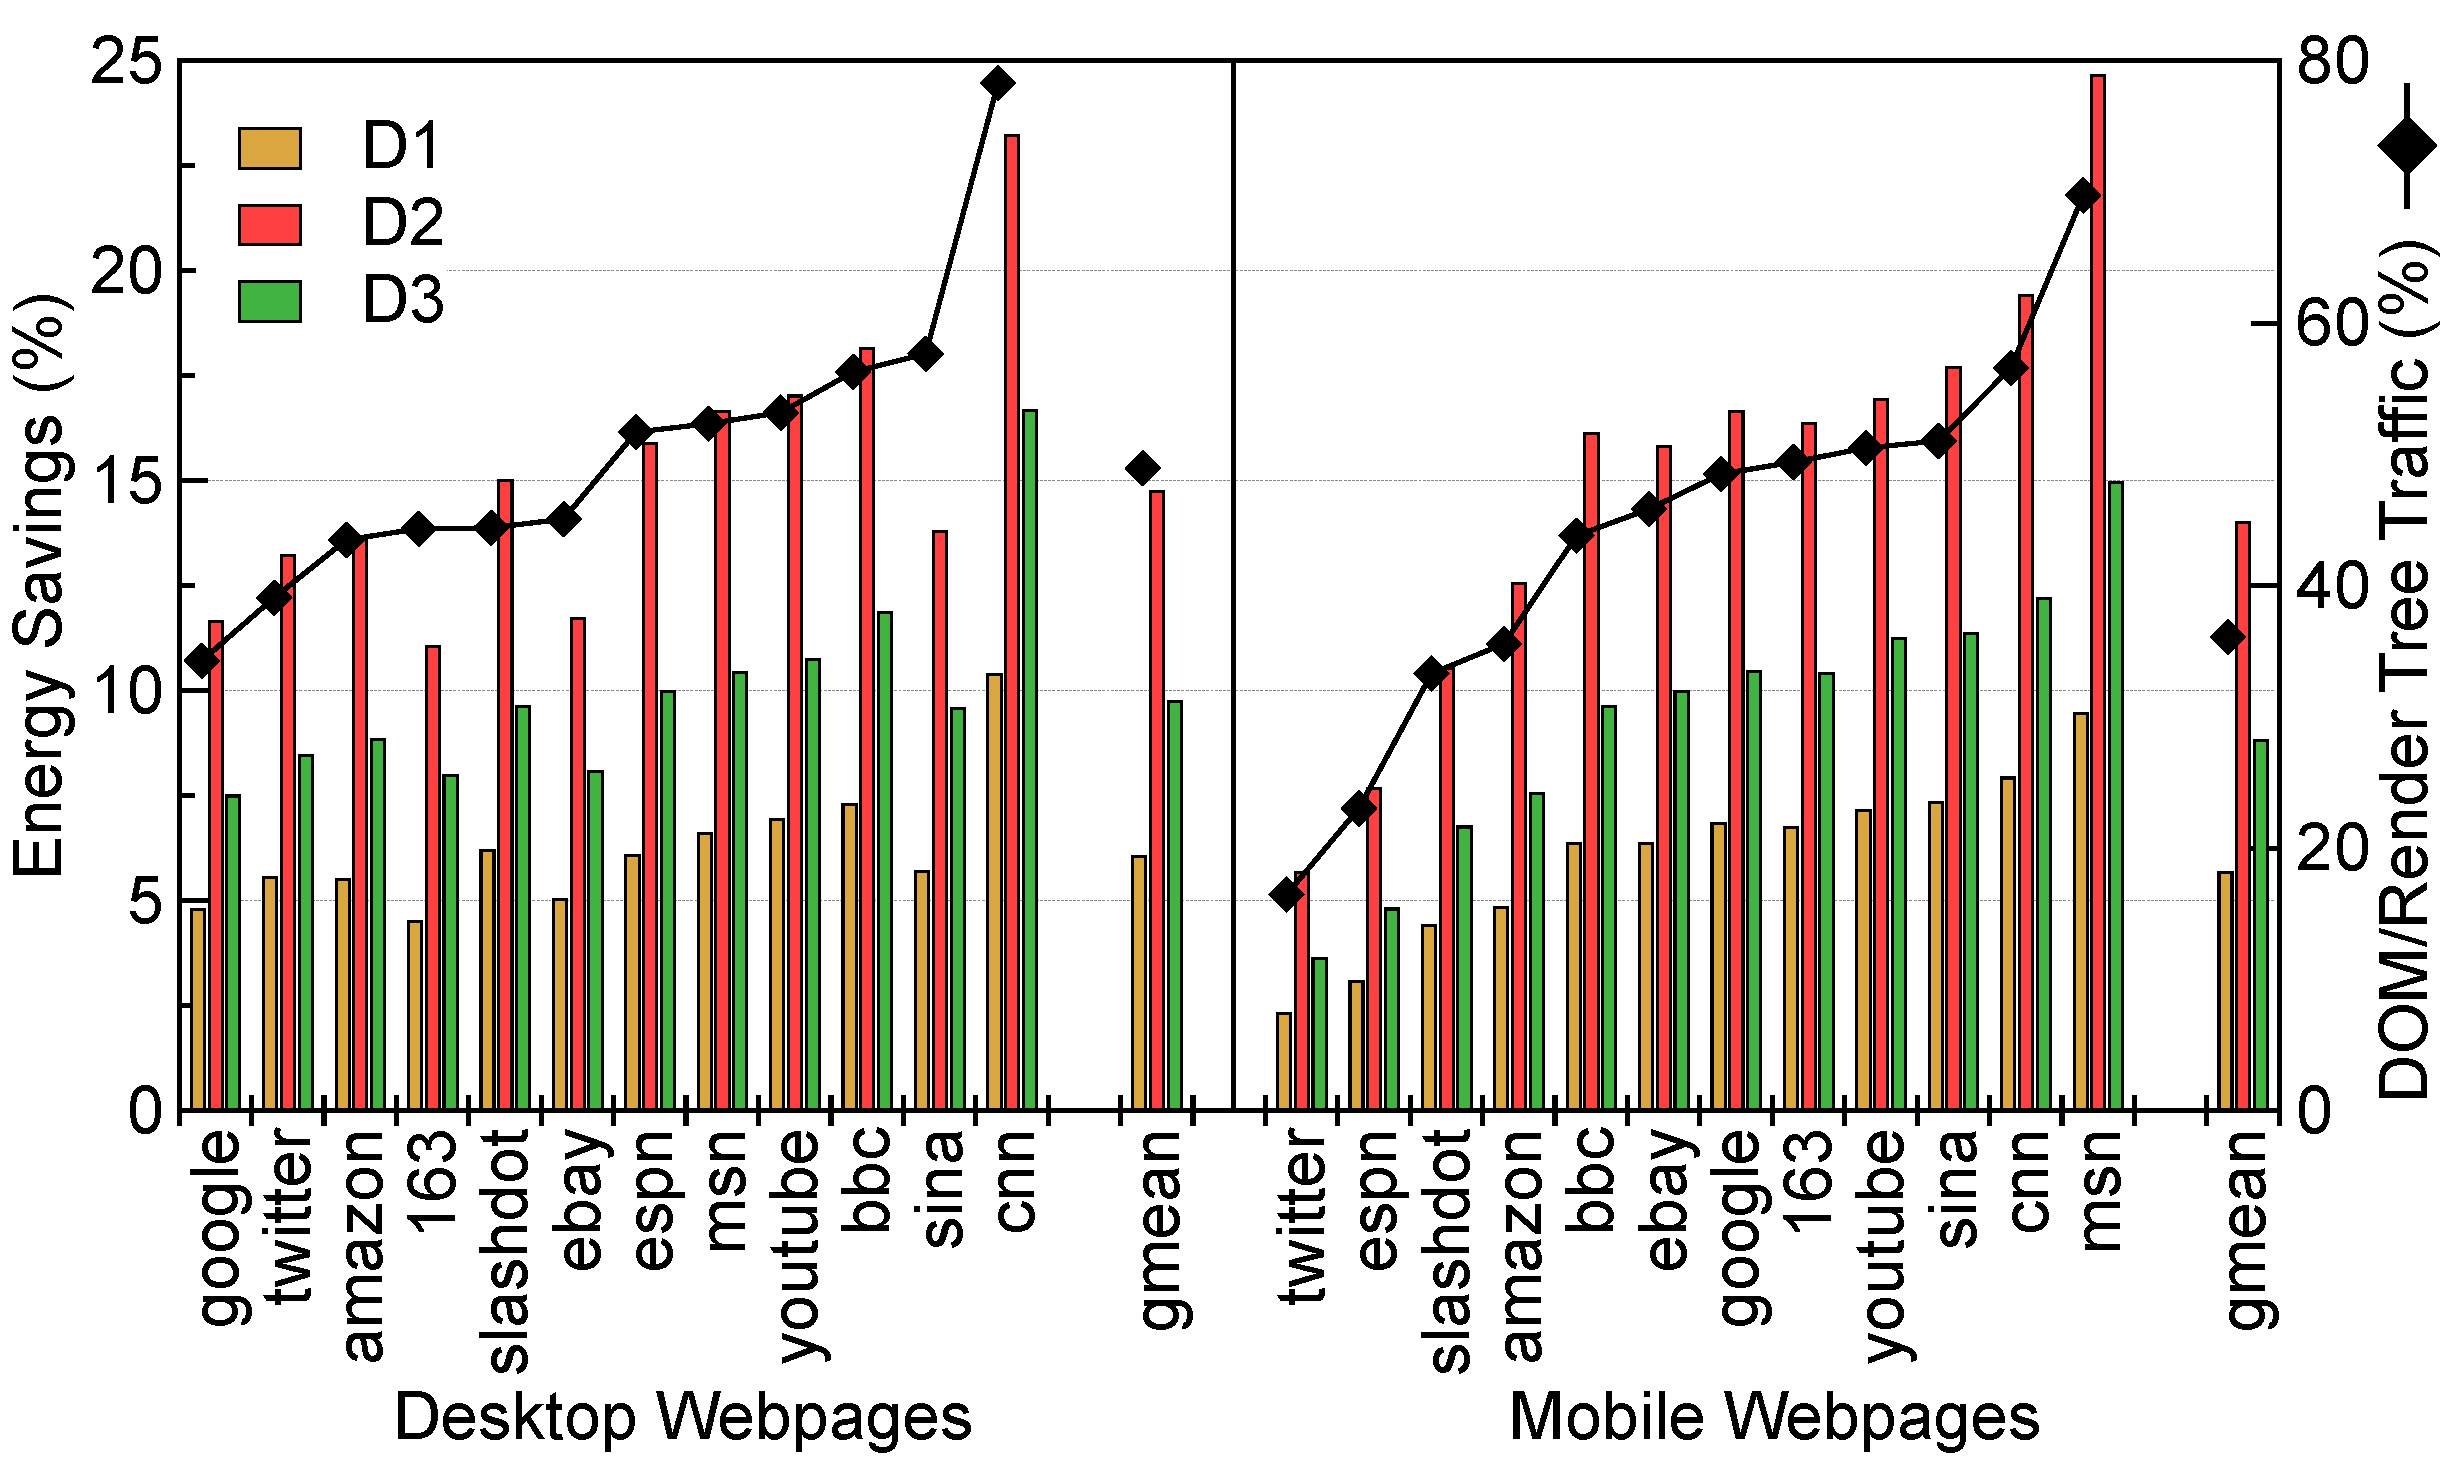
\includegraphics[trim=0 0 0 0, clip, width=\columnwidth]{cache-energy}
\caption{\small{Energy savings with a browser engine cache.}}
\label{fig:cache-energy}
\end{figure}

\begin{figure}[t]
\centering
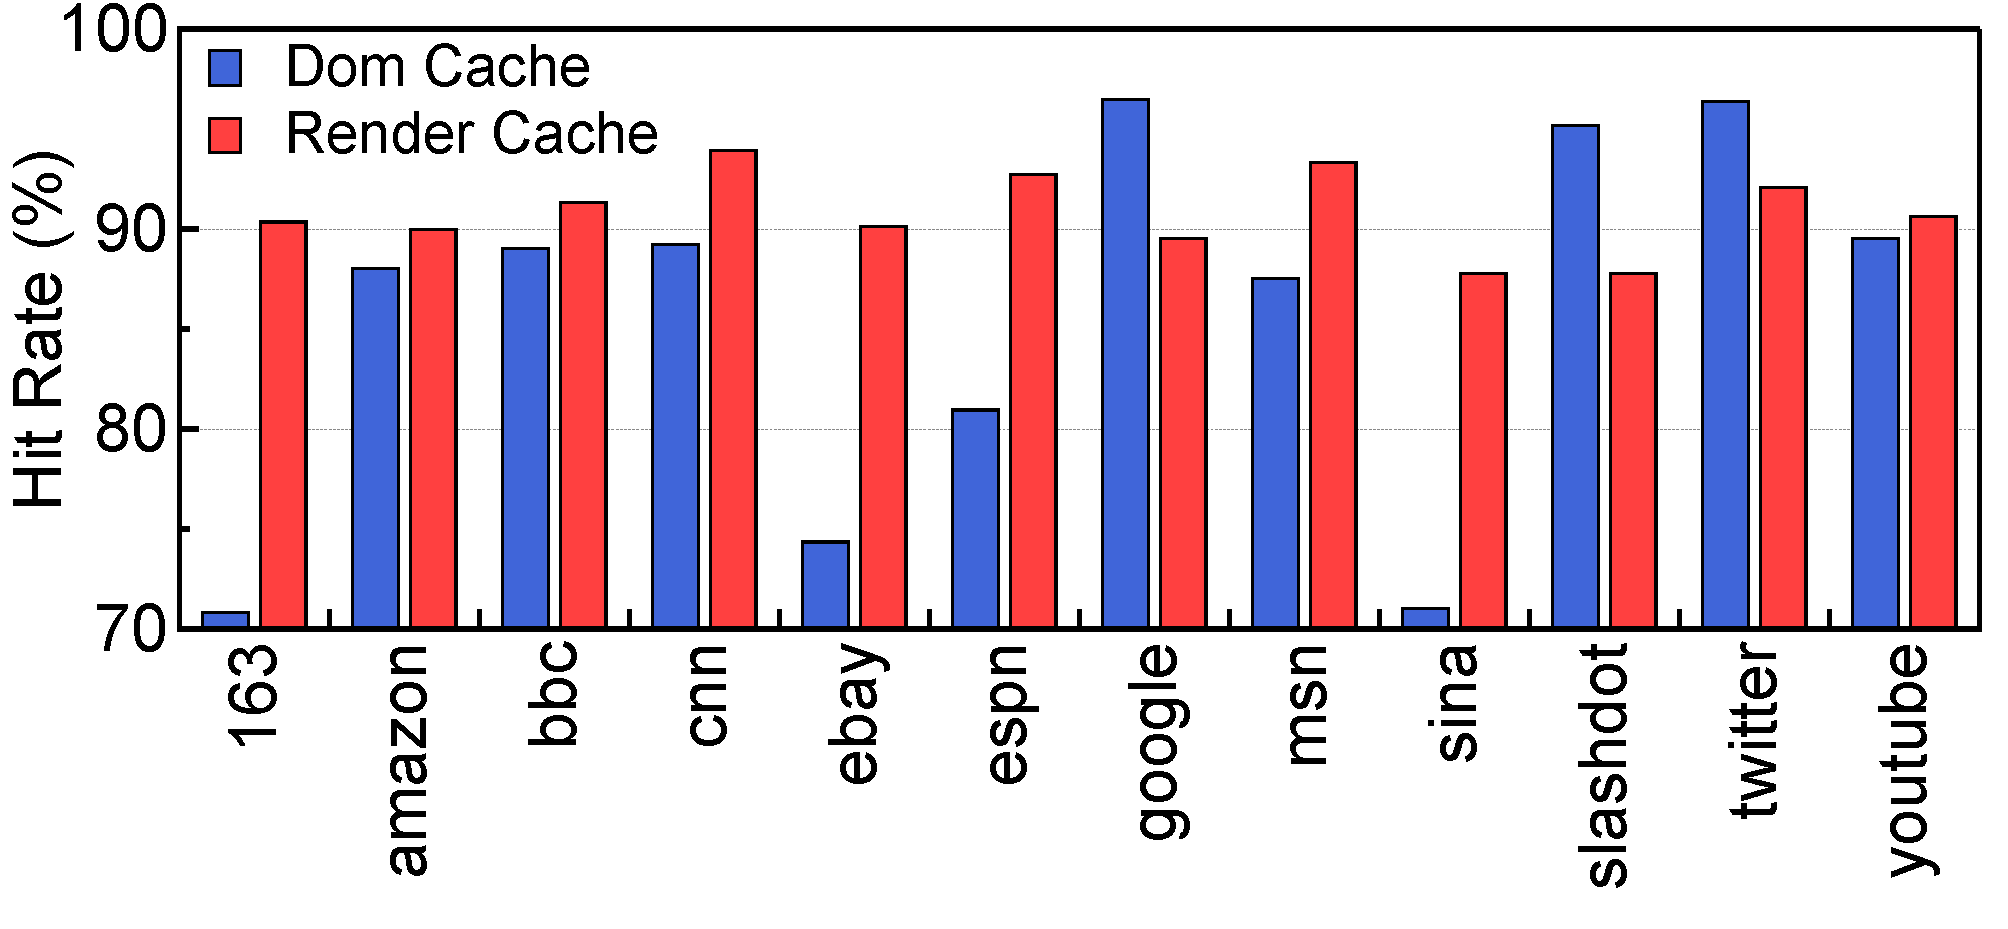
\includegraphics[trim=0 0 0 0, clip, width=.9\columnwidth]{hit-rate-page}
\caption{\small{DOM Cache and Render Cache hit rate for desktop webpages.}}
\label{fig:hit-rate-page}
\end{figure}

\begin{figure}[t]
\centering
\captionsetup{width=.9\columnwidth}
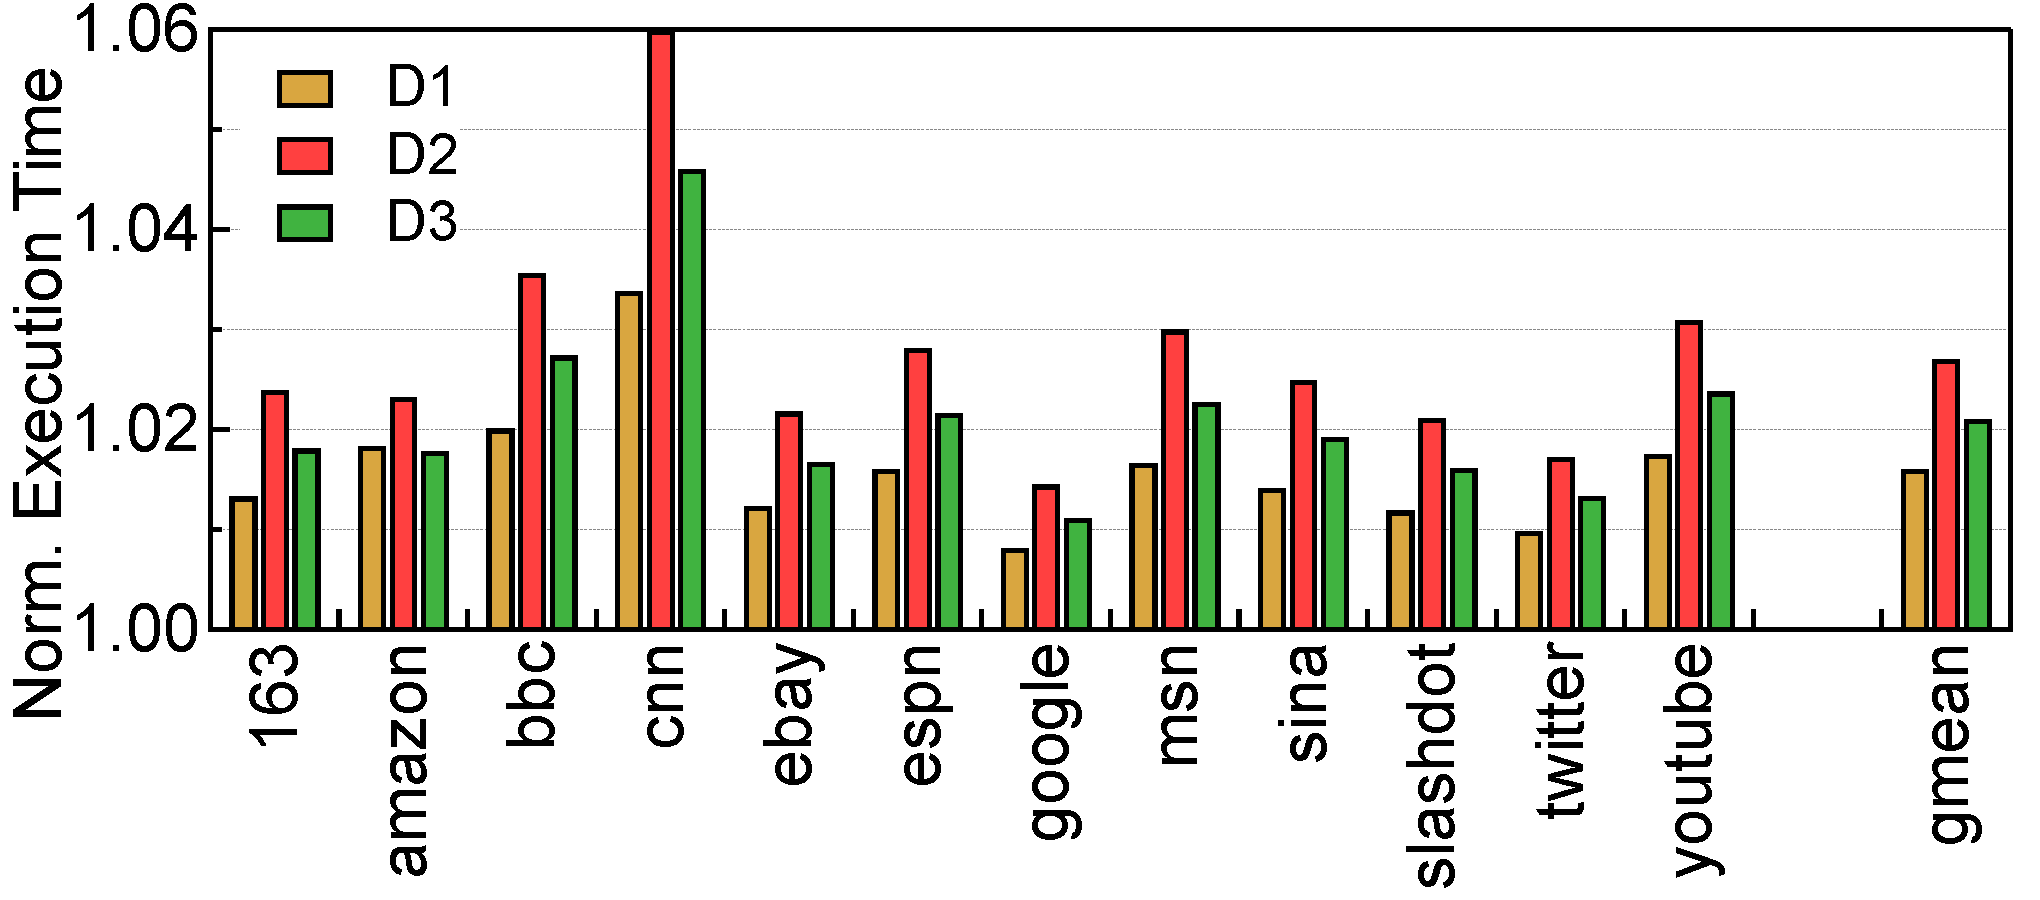
\includegraphics[trim=0 0 0 0, clip, width=.9\columnwidth]{cache-perf}
\caption{\small{Execution time with the browser engine cache of the three designs. Values are normalized to each design's baseline configuration without the browser engine cache.}}
\label{fig:cache-perf}
\end{figure}

We find that the DOM tree and Render tree access intensity largely determines the amount of energy saving. The right $y$-axis in~\Fig{fig:cache-energy} shows the amount of L1 data cache traffic that is attributed to accessing both data structures. In the most extreme case, about 80\% of the data accesses for loading~\website{cnn} touch the DOM tree and the Render tree. Therefore, it achieves the largest energy saving.

There are some outliers in desktop webpages where the energy savings are not proportional to DOM/Render tree access intensity. For example,~\website{sina} has a much higher traffic ($\sim$60\%) than~\website{twitter} ($\sim$40\%), but with similar energy savings. This is because~\website{sina} has a much lower DOM cache hit rate than~\website{twitter}. \Fig{fig:hit-rate-page} shows the DOM cache and Render cache hit ratio for desktop webpages. We observe that \website{sina} has a DOM cache hit rate at $\sim$70\%, lower than~\website{twitter} at $\sim$97\%. A lower DOM cache hit ratio indicates the \website{sina} does not fully use the low-energy browser engine cache. In contrast, we find that mobile webpages all have a high browser engine cache hit rate, and therefore their energy savings closely track the DOM/Render tree traffic.

Due to the software cache management overhead, the browser engine cache incurs performance overhead. \Fig{fig:cache-perf} shows the desktop webpages' execution time of the three designs with the browser engine cache. The values are normalized to each design's baseline configuration without the browser engine cache. We find that the performance slow down is minimal, primarily because the design decisions that we made (as described in~\Sect{sec:cache:hw}) minimize the software management overhead. On average, the slowdown for D2 with a 64~KB L1 data cache is only 2.7\%. The slowdown for D1 and D3 with smaller L1 data caches (8~KB and 32~KB, respectively) is slightly smaller--only 1.6\% and 2.1\%, respectively. We speculate that the reason is that both D1 and D3 have slower performance than D2, and as such, they amortize the overhead of the software cache management.

\subsection{Combined Evaluation}
\label{sec:arch:eval:comb}

\begin{figure}[t]
\centering
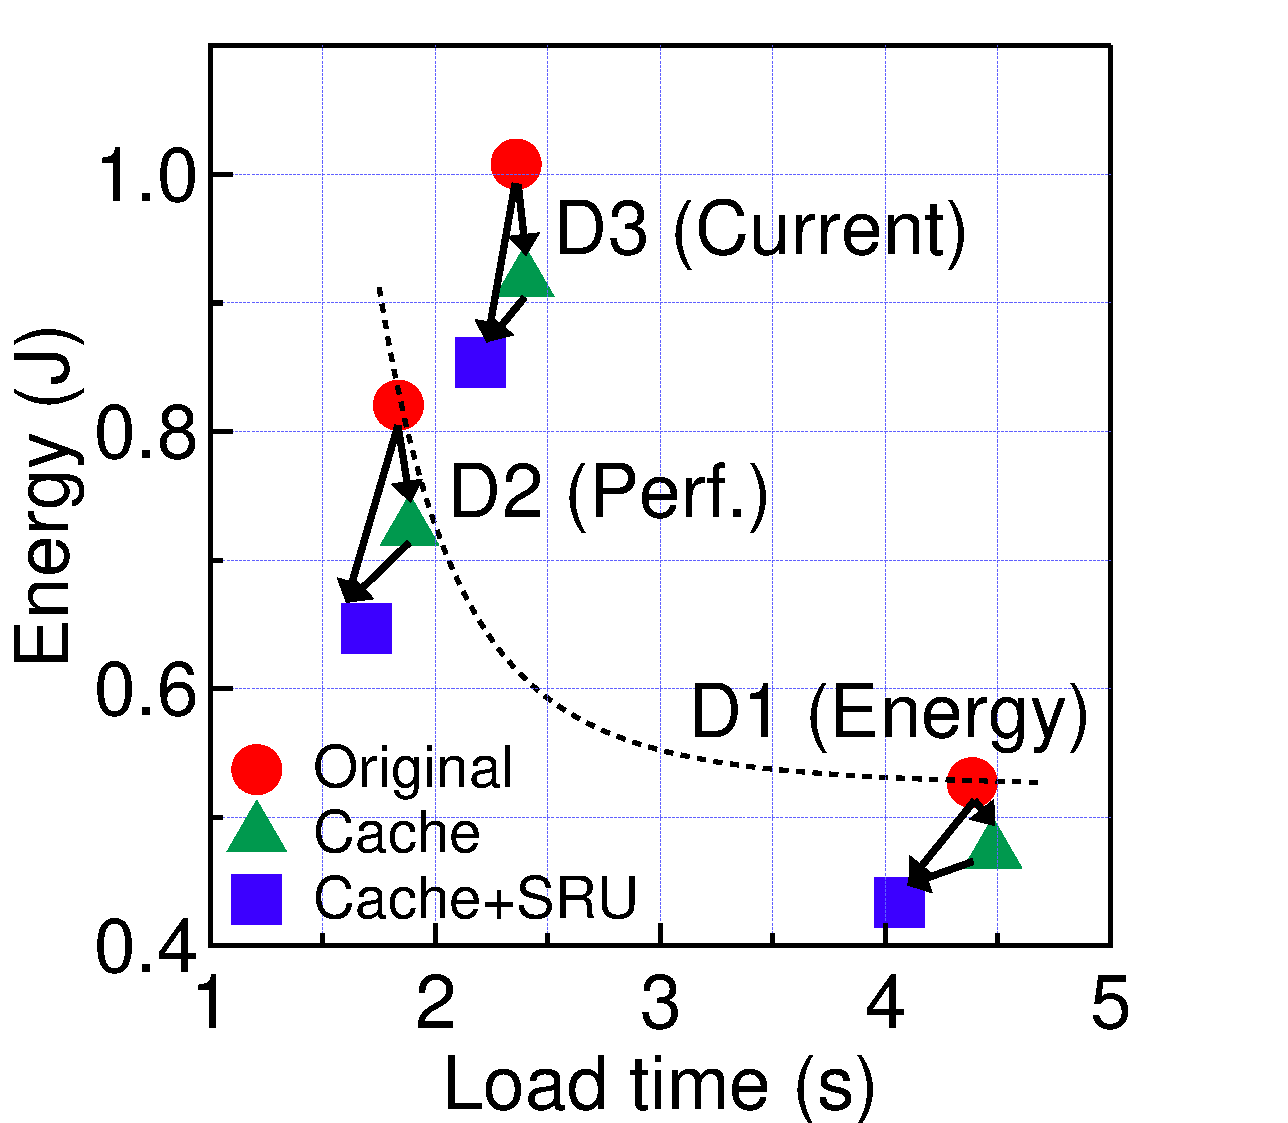
\includegraphics[trim=0 0 0 0, clip, width=.6\columnwidth]{dse-push}
\caption{Energy-efficiency improvement over three designs.}
\label{fig:dse-push}
\end{figure}

\Fig{fig:dse-push} shows the energy-efficiency improvement for the entire webpage loading on all three designs by progressively adding the two optimization techniques. The dotted curve represents the Pareto-optimal frontier of the design space discovered in~\Sect{sec:arch:customization:core}. The circles represent original designs in this energy-performance space. The triangles represent the new energy-performance trade-off points after applying the software-managed browser engine cache optimization. The squares show the new energy-performance points when the SRU is added atop the caching optimization.

Comparing the energy-conscious design (D2) with an existing mobile processor design (D3), we observe that customization of the general-purpose architecture alone without applying any specialization allows us to achieve 22.2\% performance improvement and 18.6\% energy saving.

After applying the browser engine cache, the performance slightly degrades due to its software management overhead. Therefore, all the triangles move slightly to the right despite the energy savings. However, applying the SRU optimization improves both performance and energy consumption. All the squares move toward the left corner. In effect, we push the Pareto-optimal frontier in the original design space to a new design frontier with significantly better energy efficiency.

In addition, we also observe that D3 with our specializations can now approach the original Pareto-optimal frontier. This implies that it is possible to apply specializations to existing mobile processors to achieve a similar level of energy efficiency as processors that are optimized for the mobile Web browsing workloads.

On average, the energy-conscious design (D1) benefits by 6.9\% and 16.6\% for performance improvement and energy reduction, respectively. The performance-oriented design (D2) benefits by 9.2\% and 22.2\% for performance improvement and energy reduction, respectively. Lastly, the existing mobile processor design (D3) benefits by 8.1\% and 18.4\% for performance improvement and energy reduction, respectively.

\begin{figure}[t]
\centering
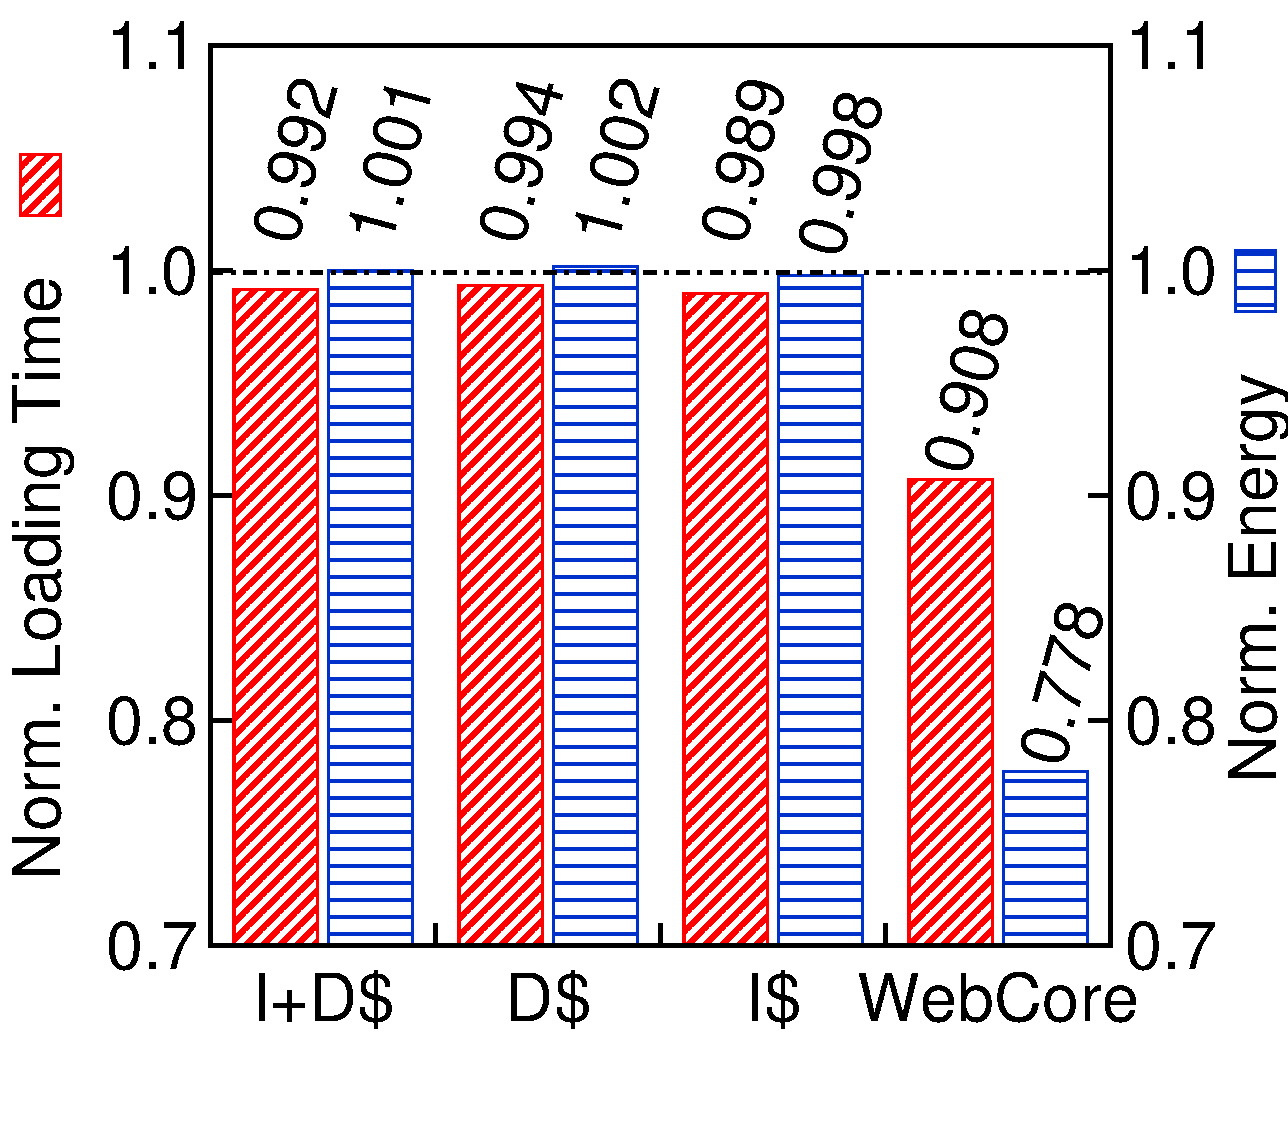
\includegraphics[trim=0 0 0 0, clip, width=.6\columnwidth]{compare-other}
\caption{Allocating area for caches versus specializations.}
\label{fig:compare-other}
\end{figure}

Our specializations incur area overhead. To quantitatively assess the effectiveness of the area overhead, we compare our results with general-purpose designs that simply use the same area overhead to scale up microarchitecture resources. In our evaluation, we use the additional area to improve the I-cache and D-cache sizes because instruction delivery and data feeding are the two major bottlenecks, as discussed in~\Sect{sec:arch:customization:sources}. The additional area would be most  justified to improve the I-cache and D-cache sizes.

As an example,~\Fig{fig:compare-other} compares our combined specializations (WebCore) with designs that increase the I-cache size by 24~KB (I\$), D-cache size by 24~KB (I\$), and both caches by 12~KB (I+D\$) based on the D2 design. The figure normalizes the webpage loading time and energy consumption to the D2 design without any specializations. We see that simply improving the cache sizes in general-purpose cores achieves only negligible performance improvement (\textless 1\%) with a slightly higher energy consumption. However, WebCore specializations provide significantly better energy efficiency.

\section{Related Work}
\label{sec:arch:related}

We first put \webcore in the broad context of architecture specialization for Web applications in \Sect{sec:arch:related:specialization}. The browser engine cache bears similarities with previous work on specialized cache design, which we discuss in \Sect{sec:arch:related:data}. Finally, \Sect{sec:arch:related:char} discusses prior work on constructing representative mobile Web benchmarks, which is inherently related to our Web application selection process.

\subsection{Architecture Specializations for the Web}
\label{sec:arch:related:specialization}

Similar to \webcore, SiChrome~\cite{SiChrome} performs aggressive specializations that map much of the Chrome browser into silicon. The key difference is that \webcore starts from a (well-optimized) general-purpose baseline and thus retains general-purpose programmability while still being energy-efficient. In addition, SiChrome evaluates energy-efficiency using the EDP metric while our Pareto optimal analysis provides a more generic optimization view than EDP.

EFetch~\cite{efetch} and ESP~\cite{esp} also propose specialized hardware structures on top of general-purpose cores to improve the performance and energy-efficiency of Web applications. They view a Web application execution as a sequence of events. As a result, the proposed specialized hardware primarily targets the inefficiencies associated with the event-driven execution model. \webcore views a Web application execution as a mix of different kernels. As such, the proposed specialization technique targets individual kernels. Both views are complementary in that per-event execution can benefit from kernel-level improvement that \webcore provides and vice versa.

\subsection{Specialized Cache Design}
\label{sec:arch:related:data}

L0 caches and scratchpad memories~\cite{filtercache,scratchpad} have long been used to reduce data communication overhead by acting as small, fast, and energy-conserving data storage. The browser engine cache proposed in this paper demonstrates the effectiveness of such an idea for mobile Web browsing workloads. We propose to implement the browser engine cache as a collection of registers where each register holds exactly one DOM (render) tree attribute. In contrast, the typical L0 cache in mobile SoCs~\cite{krait} is agnostic to the application-level data structures. Each L0 cache line, thus, holds more than one DOM attribute, leading to excessive energy consumption when accessing individual attributes.

In addition, the strong locality of the principal data structures revealed in our analysis can potentially be captured by dedicating cache ways to the Web browser application~\cite{BIC,WayStealing}. The streaming access pattern of the DOM tree shown in~\Fig{fig:data-acs} indicates that a dynamic cache insertion policy such as DIP~\cite{dip} or an intelligent linked data structure prefetcher~\cite{LDS} on L1 data cache are also worth exploring. However, the browser engine cache we propose aims at saving energy with minimal loss in performance, which the prior performance-oriented techniques have not been proven/claimed to provide.

\subsection{Web Applications Characterization}
\label{sec:arch:related:char}

BBench~\cite{BBench} is a webpage benchmark suite that includes 11 hot webpages. Its authors perform microarchitectural characterizations of webpage loading on an existing ARM system. Although the authors show that the 11 webpages have distinctly different characteristics from SPEC CPU~2006, they do not quantify the comprehensiveness and representativeness of the webpages against the vast number of webpages ``in the wild.'' In stark contrast, our analysis in~\Sect{sec:arch:exp} systematically proves the broad coverage of our webpages, which is needed for robustly evaluating the impact of the optimizations that we propose. For example, we find that BBench does not include significantly complex webpages, and our analysis led to including two webpages of that sort, i.e., ~\website{www.163.com} and~\website{www.sina.com.cn}. Their webpage sizes are about 4x larger than the average BBench webpage, and as such are needed to increase the coverage of our benchmarking suite.

MobileBench~\cite{mobilebench} characterizes the performance impact of various microarchitecture features on mobile workloads. Our paper quantifies the performance-energy trade-off, and focuses specifically on Web applications. Complementary to our design space exploration, MobileBench results show that more aggressive customizations of other microarchitecture structures such as the prefetcher are worth exploring.

%!TEX root=../paper.tex

\chapter{WebRT: Smart Web Browser Runtime Optimizing for Energy-Efficiency}
\label{sec:runtime}

Today's mobile processors are becoming extremely heterogeneous. They often combine general-purpose cores that have different performance and energy characteristics~\cite{single-ISA} (e.g., asymmetric chip-multiprocessor architecture) with special-purpose domain-specific cores (e.g., \webcore). While the hardware upheaval promises performance and energy improvements for the mobile Web, current Web runtime systems are not designed to fully exploit the capability of the underlying hardware. The main bottleneck is that current runtime-architecture interface merely exposes the hardware as a monolithic sequential execution model to the runtime system while hiding many architecture-level details. Without having a full visibility of the hardware details, current Web runtimes often lead to energy-inefficient decisions or violate user QoS requirement.

To bridge the widening gap between the architecture complexity and the architecture-agnostic runtime system, I propose to enhance the existing runtime-architecture interface by exposing architecture details to the Web runtime. I specifically focus on the ACMP architecture~\cite{acmp,single-ISA} as the hardware substrate. ACMP is long known to provide a large performance-energy trade-off space, and is already widely used in today's mobile systems~\cite{big-little-future,exynos5biglittle}. I  quantitatively show that Web applications particularly benefit from the heterogeneity offered by the ACMP architecture to achieve an ideal balance between QoS experience and energy consumption.

Leveraging the ACMP architecture, I propose \webrt, a Web runtime that minimizes energy while guaranteeing satisfactory user QoS experience by scheduling Web application executions using proper ACMP configurations. The key insight is that we must devise different optimization schemes according to the nature of different user interaction forms. To that end, I introduce a user-application interaction model called LTM. LTM captures three fundamental user interaction forms in mobile Web applications--Loading, Tapping, and Moving--and provides a framework for reasoning about different energy optimization strategies.

The rest of this chapter is organized as follows. \Sect{sec:runtime:exp} presents the hardware and software experimental methodology. \Sect{sec:runtime:ltm} introduces the LTM interaction model and points out that the runtime mechanisms need to be different for different interaction forms. Using loading (L) as a case study, \Sect{sec:runtime:char} quantitatively shows that an ACMP is beneficial for mobile Web and therefore is a natural candidate for \webrt. \Sect{sec:runtime:load} describes the \webrt components for L, and \Sect{sec:runtime:ebs} describes the \webrt component for T and M. Finally, \Sect{sec:runtime:related} compares the contrasts \webrt with prior work on software support for mobile Web.

\section{Experimental Setup}
\label{sec:runtime:exp}

\paragraph{Software Infrastructure} \webrt-related experiments and implementations are performed on Google's open-source Chromium browser engine, which is used directly in the Chrome browser and is the core of many other popular browsers, such as Opera and Android's default browser. We use Chromium version 48.0.2549.0, which is the most recent version at the time of my work. The modified Chromium runs on unmodified Android version 4.2.2.

\paragraph{Hardware Platform} We use the ODroid XU+E development board~\cite{odroidxue}, which contains an Exynos 5410 SoC that is known for powering the Samsung Galaxy S4. The Exynos 5410 SoC contains a representative ACMP architecture comprising an energy-hungry high-performance (big) core cluster and an energy-conserving low-performance (little) core cluster. The big and little clusters can be individually disabled and enabled. The big cores are ARM Cortex-A15 processors that operate between 800~MHz and 1.8~GHz at a 100~MHz granularity. The little cores are ARM Cortex-A7 processors that operate between 350~MHz and 600~MHz at a 50~MHz granularity. The frequency switching and core migration overhead is \SI{100}{\mu\second} and 20~$\mu$s, respectively~\cite{big-little,ebs}.

\paragraph{Energy Measurement}  \webrt focuses on the processor power consumption because the processor power has been steadily increasing and has gradually become the most significant power consumer in a mobile device compared to other components such as the screen and radio (\Sect{sec:motivation:energy}).

We measure the processor power and energy consumption on real hardware as follows. The ODroid XU+E development board has built-in current sense resistors (\SI{10}{\milli\ohm}) for both the big and little cores. We use a National Instrument DAQ Unit X-series 6366 to collect voltage measurements at these sense resistors for the big and small CPU clusters at a rate of 1,000 samples per second, and thereby derive the power consumption. Energy consumption is computed by multiplying power with real execution time.

\paragraph{Reproducibility} We repeat every experiment that we study 3 times. Unless otherwise mentioned, the results we report are the median of all runs. We find the run-to-run variations are usually about 5\%, and do not affect our conclusions. We use Mosaic~\cite{mosaic}, a UI-level record and replay tool, to ensure consistent user interaction and to reduce human-induced noise across different runs on the same application.

\section{LTM Model of Mobile User Interaction}
\label{sec:runtime:ltm}

%An ACMP consists of cores with different microarchitectures, such as out-of-order and in-order. Each core has a variety of frequency settings. Different core and frequency combinations provide a large trade-off space between performance and energy. The objective of our ACMP-based \webrt is to find an ideal ACMP configuration (i.e., a $\langle core, frequency \rangle$ tuple) that minimizes the energy consumption while guaranteeing an acceptable responsive time when a user interaction happens.

\begin{figure}[t]
  \centering
  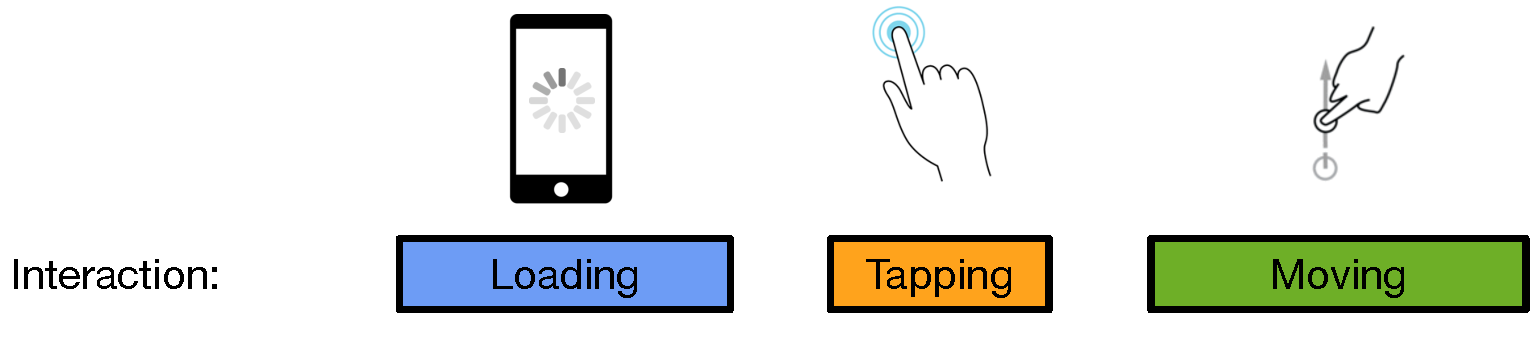
\includegraphics[trim=0 0 0 0, clip, width=.9\columnwidth]{interaction_model}
  \caption{The LTM (Loading-Tapping-Moving) user-application interaction model of mobile Web. LTM captures three primitive types of interaction: page loading, finger tapping, and finger moving. We use LTM as a framework to reason about user QoS experience.}
  \label{fig:interaction}
\end{figure}

To systematically analyze user interactions in mobile Web applications, we introduce a simple conceptual model called LTM, which captures three primitive user interaction forms in mobile Web applications: loading application page (L), tapping the display (T), and moving finger on the display (M). \Fig{fig:interaction} illustrates the LTM model.

The three interactions cover a majority of human-computer interactions on mobile devices. This is because every application requires a loading phase (L), and post-loading interactions on mobile devices are mostly performed in the form of finger tapping (T) or finger moving (M). The moving interaction in particular could be manifested in various ways, such as scrolling, swiping, or even drawing a picture. Internally, each user interaction is translated to one or more application event. For example, a tapping interaction is often translated to a \texttt{touchstart} and a \texttt{touchend} event, and a moving interaction can be translated to a \texttt{scroll} event or a \texttt{touchmove} event depending on context. In this paper, we focus on the following events that could be triggered by LTM interactions on a mobile device: \texttt{click}, \texttt{scroll}, \texttt{touchstart}, \texttt{touchend}, and \texttt{touchmove}. We do not consider events specific to desktops (e.g., \texttt{drag}, \texttt{mouseover}) that are generally not fired on mobile devices.

%Each event is bound to a DOM node with a callback function, which is executed when the event is triggered on the associated DOM node. The result of callback execution is fed into the Web browser rendering engine, which eventually paints the resulting frame(s) and updates the display. Frames are what users perceive as application's responses to their interactions, and thus determine the QoS experience.

The runtime optimization strategy for Loading is different from that for Touching and Moving. The fundamental difference is that Loading occurs only once per usage session while Touching and Moving interactions occur repetitively throughout the entire Web application usage session. As a result, it is possible to make the prediction for the Touching and Moving interactions based on the history information within the same usage session. For Loading, however, every application loading is likely different from the previous one, and as such we can not make predictions based on previous loadings of (potentially different) applications. Instead, we have to make prediction based on the particular content of a given Web application. I will discuss the \webrt component that targets the Loading in \Sect{sec:runtime:load} and the component that targets Touching and Moving interactions in \Sect{sec:runtime:ebs} separately.

\section{Motivation: Energy-Delay Trade-off}
\label{sec:runtime:char}

%Our goal in this work is to meet the cut-off latency of webpage loading while minimizing the energy consumption under that constraint whenever possible.  In order to achieve that, we have to carefully balance the performance and energy consumption of webpage loading. Heterogeneous systems with big/little cores each with DVFS capabilities naturally enable a flexible balance between performance and energy due to a large scheduling space.  Different workloads, according to their behaviors, can be scheduled to different cores/frequencies to explore different trade-offs between performance and energy.

%Our goal in this work is to meet the cut-off latency of webpage loading while minimizing the energy consumption under that constraint whenever possible.

An ACMP consists of cores with different computation capabilities--often with different microarchitectures, such as big out-of-order cores and small in-order cores. Each core has a variety of frequency settings. Different core and frequency combinations provide a wide range performance and energy characteristics. The flexibility of an ACMP architecture to make trade-offs between performance and energy consumption leads us to answer a fundamental question: do Web applications benefit from an ACMP heterogeneous systems?  For example, can a processor lower the frequency for a simple webpage to consume less energy but still respect the QoS deadline? Can a webpage originally scheduled on an energy-consuming core be migrated to an energy-saving core without violating the QoS constraint?

We quantitatively answer this question using webpage loading as a case study. The same experimental methodology and conclusion also hold true for the other two types of interactions in mobile Web applications. We base our measurements and analysis on the 5,000 hottest webpages on the Internet ranked by \website{http://www.alexa.com/}. We show that different webpages require different core and frequency configurations to meet a given deadline of webpage loading while minimizing the energy. This suggests that ACMPs with both big and smalls core, each capable of performing DVFS, are strongly beneficial.

To demonstrate the benefits of such heterogeneous systems, we measure the webpage load time and energy consumption of the 5,000 webpages on the Cortex-A9 and A8 processors. We sweep a total of seven configurations available on the big and little cores, i.e., Cortex-A9 with four DVFS settings and A8 with three DVFS settings, respectively. We begin our analysis with four webpages that represent the general trends that we observe (\Sect{sec:runtime:char:representative}), and we subsequently expand our analysis to include the comprehensive set of all webpages (\Sect{sec:runtime:char:comprehensive}).

\subsection{Representative Analysis}
\label{sec:runtime:char:representative}

\Fig{fig:pareto} shows the energy versus delay plots for the four representative webpages. Assuming 3~seconds as the cut-off latency for webpage load~\cite{ThreeSecond}, the four webpages have different ideal core and frequency configurations to meet the cut-off while simultaneously minimizing the energy consumption. For example, \website{www.autoblog.com} is a complex website that has 4,235 nodes in the DOM tree, and it therefore requires the highest frequency on the big core to meet the cut-off latency. However, this configuration is overpumped for simpler websites such as \website{www.newegg.com} with 3,152 DOM tree nodes. It only requires 700~MHz of the big core. This suggests that some webpages can benefit from different frequencies in each processor's core.

\begin{figure}[p]
\centering
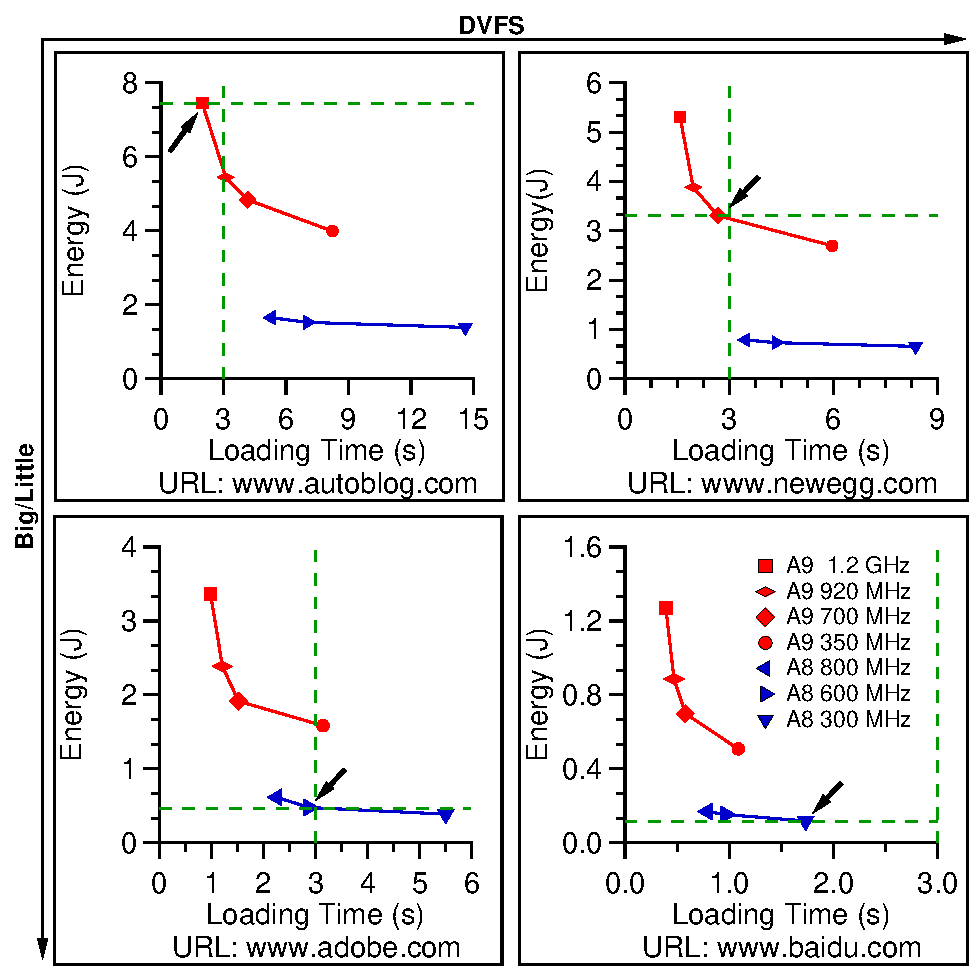
\includegraphics[trim=0 0 0 0, clip, width=\columnwidth]{pareto}
\caption{Webpages have different ideal execution configurations to meet the cut-off latency while consuming the least energy.}
\label{fig:pareto}
\end{figure}

In addition, some webpages can take advantage of scheduling between big/little cores. If only the big core is available, \website{www.adobe.com} can at best be loaded at 700~MHz. Instead, with the little core, the webpage can be loaded using 600~MHz, which still meets the cut-off latency but consumes 75\% less energy than 700~MHz on the big core. Similarly, \website{www.baidu.com} is a search engine website that has very concise content with less than 1~KB of images. It only requires the lowest frequency on the little core.

\subsection{Comprehensive Analysis}
\label{sec:runtime:char:comprehensive}

We extend our analysis to the full set of 5,000 webpages. \Fig{fig:conf-dist} shows the distribution of ideal core and frequency configurations for different cut-off latencies, ranging from 1~second to 10~seconds at 1~second intervals. Each region in \Fig{fig:conf-dist} represents the portion of webpages that are loaded at the corresponding architectural configuration with minimal energy consumption while still meeting the cut-off latency. We find a wide distribution of ideal configurations, indicating the benefits of a flexible baseline architecture that mixes big/little cores with different frequencies. 
%For example, if the cut-off latency is 1~s, the big core with its peak frequency can load 52.6\% of the webpages successfully while consuming the least amount of energy compared to all the other configurations.

\begin{figure}[t]
\centering
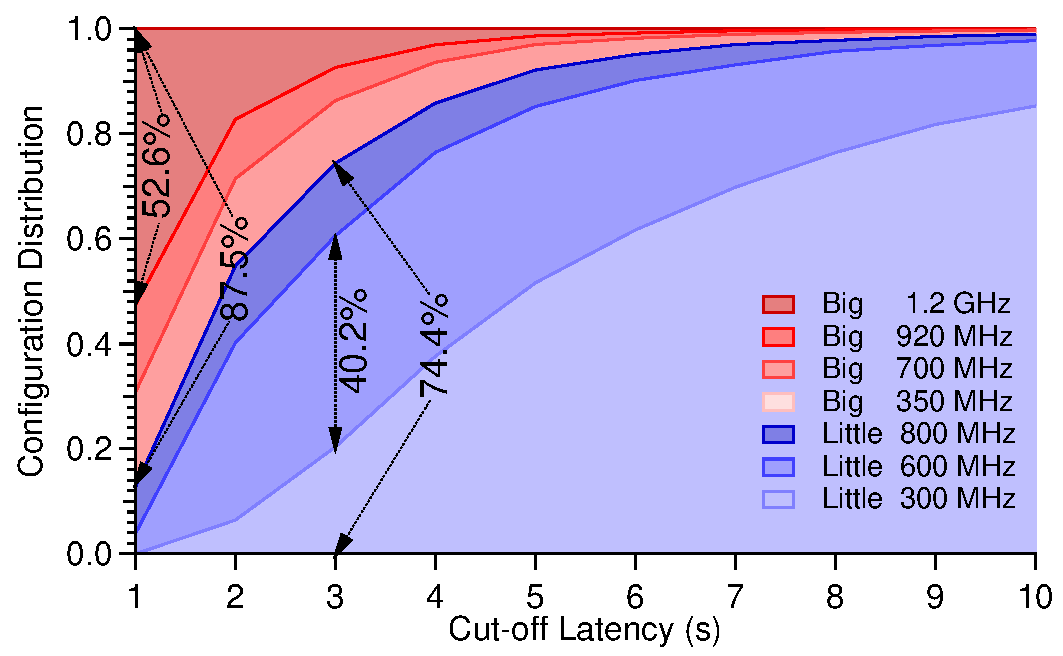
\includegraphics[trim=0 0 0 0, clip, width=.9\columnwidth]{conf_dist}
\caption{The distribution of ideal core and frequency configurations under different cut-off latencies.}
\label{fig:conf-dist}
\end{figure}

Assuming a tight 3~second cut-off latency~\cite{ThreeSecond}, a single core with a fixed frequency is insufficient for a wide spectrum of webpages.  The best single core with a fixed frequency is the little core with 600~MHz.  However, it can only load 40.2\% of the webpages within that latency constraint. Even a single core (big or little) with varying frequencies is insufficient. When we consider the little core with varying frequencies, only 74.4\% of webpages can be loaded within the cut-off latency. However, if we use a big core to load all the webpages, then the 74.4\% of webpages have suboptimal performance-energy trade-off. Furthermore, a simple heterogeneous system with both a big and little core but each with a fixed frequency may also cause suboptimal performance-energy trade-off for some webpages. Statistically, the best single-frequency configurations are 700~MHz on the big core and 600~MHz on the little core; yet, a heterogeneous system with only these two settings leads to ideal scheduling for only 52.1\% of the webpages.

Although 3~seconds is the typical cut-off latency on mobile systems, we also study the sensitivity of the ideal configuration distribution under other cut-off latencies. We find that varying cut-off demands also call for a flexible baseline architecture. As \Fig{fig:conf-dist} shows, no one particular configuration consistently performs well under varying cut-off latency requirements. For example, although relaxed cut-offs favor the little core, it is suboptimal for 87.5\% of the webpages under a tight 1~second constraint. Similarly, the big core, which performs very well under tight cut-offs, is overpumped under more relaxed constraints; it is only needed for about 3\% of webpages when the cut-off latency is 10~seconds.

%In conclusion, different webpages have different ideal core and frequency configurations, and can strongly benefit from a versatile heterogeneous system consisting of both big and little cores each capable of performing DVFS.
In summary, we find that different webpages require different ideal core and frequency settings to achieve the ideal balance between performance and energy-efficiency. Varying cut-off latencies also demand different ideal configurations. Therefore, we conclude that different webpages can strongly benefit from a versatile heterogeneous system consisting of both big and little cores each capable of performing DVFS.

\section{Webpage-aware Scheduling}
\label{sec:runtime:load}

In this section, I first show that it is possible to predict the webpage load time and energy consumption using merely webpage-inherent characteristics (\Sect{sec:runtime:load:model}). This prediction scheme had two advantages. First, it does not rely on any previous webpage loading history information and is based completely on each webpage's inherent characteristics. Second, the prediction is performed at the webpage parsing time which happens at the very beginning of the loading process, and as such allows enough time for energy optimizations. We quantitatively show that our predictive models achieve a desirable accuracy (\Sect{sec:runtime:load:model_eval}).

Based on such predictions, we propose a webpage-aware scheduler as a \webrt component that predicts the ACMP configuration for webpage loading in order to minimize energy consumption while meeting a specified cut-off latency (\Sect{sec:runtime:load:sched}). Real hardware and software measurements show that against a performance-oriented hardware strategy, the webpage-aware scheduler achieves 83.0\% energy savings while violating the cut-off latency for only 4.1\% more webpages. Compared with a more intelligent, on-demand OS DVFS scheduler, the mechanism achieves an additional 8.6\% energy savings along with a 4.0\% performance improvement~(\Sect{sec:runtime:load:eval}).

\subsection{Performance and Energy Modeling}
\label{sec:runtime:load:model}

%!TEX root=../../paper.tex

\begin{table}[t]
\centering
\captionsetup{width=.9\columnwidth}
\renewcommand*{\arraystretch}{1.4}
\renewcommand*{\tabcolsep}{15pt}
\resizebox{.9\columnwidth}{!}{
\begin{tabular}{ll}
\toprule[0.15em]
\multicolumn{1}{l}{\bigstrut\textbf{Category}} & \multicolumn{1}{l}{\textbf{Model Predictors}}\\
\midrule[0.05em]
\multicolumn{1}{l}{\multirow{3}{*}{Webpage primitive: HTML}}
                &       Number of each tag \\
                &       Number of each attribute\\
                &       Number of DOM tree node\\
\midrule[0.05em]
\multicolumn{1}{l}{\multirow{3}{*}{Webpage primitive: CSS}}
                &       Number of rules \\
                &       Number of each selector pattern\\
                &       Number of each property \\
\midrule[0.05em]
\multicolumn{1}{l}{\multirow{2}{*}{Content-dependent}}
                &       Total image size \\
                &       Total webpage size \\
\bottomrule[0.15em]
\end{tabular}
}
\caption{Model Predictors}
\label{tab:feat_list}
\end{table}



\paragraph{Model Derivation} We find that regression models provide sufficient accuracy to predict the webpage load time and energy consumption. A regression model is a mathematical function between a set of predictors and a response. Within our context, the response is either the webpage's load time or energy consumption in loading the webpage. The predictors are a set of webpage characteristics. The linear regression model models a webpage's load time and energy consumption (responses) as a linear combination of various webpage characteristics (predictors), formulated as: $y = \beta_0 + \sum_{i=1}^{p} x_i \beta_i$ where \textit{y} denotes the response, \textit{$x = x_{1},...,x_{p}$} denote \textit{p} predictors, and \textit{$\beta = \beta_{0},...,\beta_{p}$} denote corresponding coefficients of each predictor. The \textit{least squares method} is used to identify the best-fitting $\beta$ that minimizes the residual sum of squares (RSS)~\cite{ESL}.

We consider two types of predictors. The first type includes the \textit{webpage-inherent} primitives such as the number of HTML tags. These primitives have show strong inter-webpage differences, and as such have a strong influence on the load time and energy consumption. In addition, we must also consider the impact of \textit{content-dependent} characteristics such as image size and the total size of a webpage. These characteristics are coarse-grained metrics that are independent of webpage structures but which influence the load time and energy of rendering. A media website is a classic example where content-dependent characteristics are dominant. For example, a news website, such as \website{www.bbc.com}, has a relatively stable appearance. Its structural layout (i.e., HTML) and style (i.e., CSS) do not change frequently. However, the website's content is changing daily to keep up with the latest breaking news. For instance, they are constantly updating images, and image sizes have a significant impact on the webpage load time. In our measurement we observe a 4X load time difference between a 200~KB and 50~KB image. Therefore, it is necessary to consider both webpage-primitive and content-dependent characteristics for modeling the load time and energy consumption of webpage load.

We summarize these features in \Tbl{tab:feat_list}. In total, we consider 376 predictors. We require a number of sampling observations to construct the regression models. In total, we obtain 2,500 sampling observations, for which we measure both webpage load time and energy consumption simultaneously on the Cortex-A9 processor running at 1.2 GHz.
 
\paragraph{Model Specification and Refinement} We apply various techniques to mitigate overfitting and capture predictor-response nonlinearity to achieve high prediction accuracy. We use R~\cite{R} and its \textit{glmnet} and \textit{rms} packages for all analysis.

We consider a large number of predictors (376) relative to the number of observations (2,500). This is known to produce predictions that result in overfitting~\cite{ESL}. We mitigate this, to the first order, by eliminating predictors that are less correlated to the response. We test the predictor/response correlation strength by calculating the squared correlation coefficient ($\rho^2$) between each predictor variable and observed load time and energy. \Fig{fig:pred-strength} shows the seven most-correlated predictors. For both load time and energy, we find the number of DOM tree nodes (\textsf{\#nodes}) is the most-correlated webpage primitive because it heuristically captures the webpage structure's complexity. Also, both image size and the total webpage size are also correlated because they capture the webpage content. We only select predictors with $\rho^2$ greater than 0.01.

\begin{figure}[t]
\subfloat[Predictor-response correlation.]{
  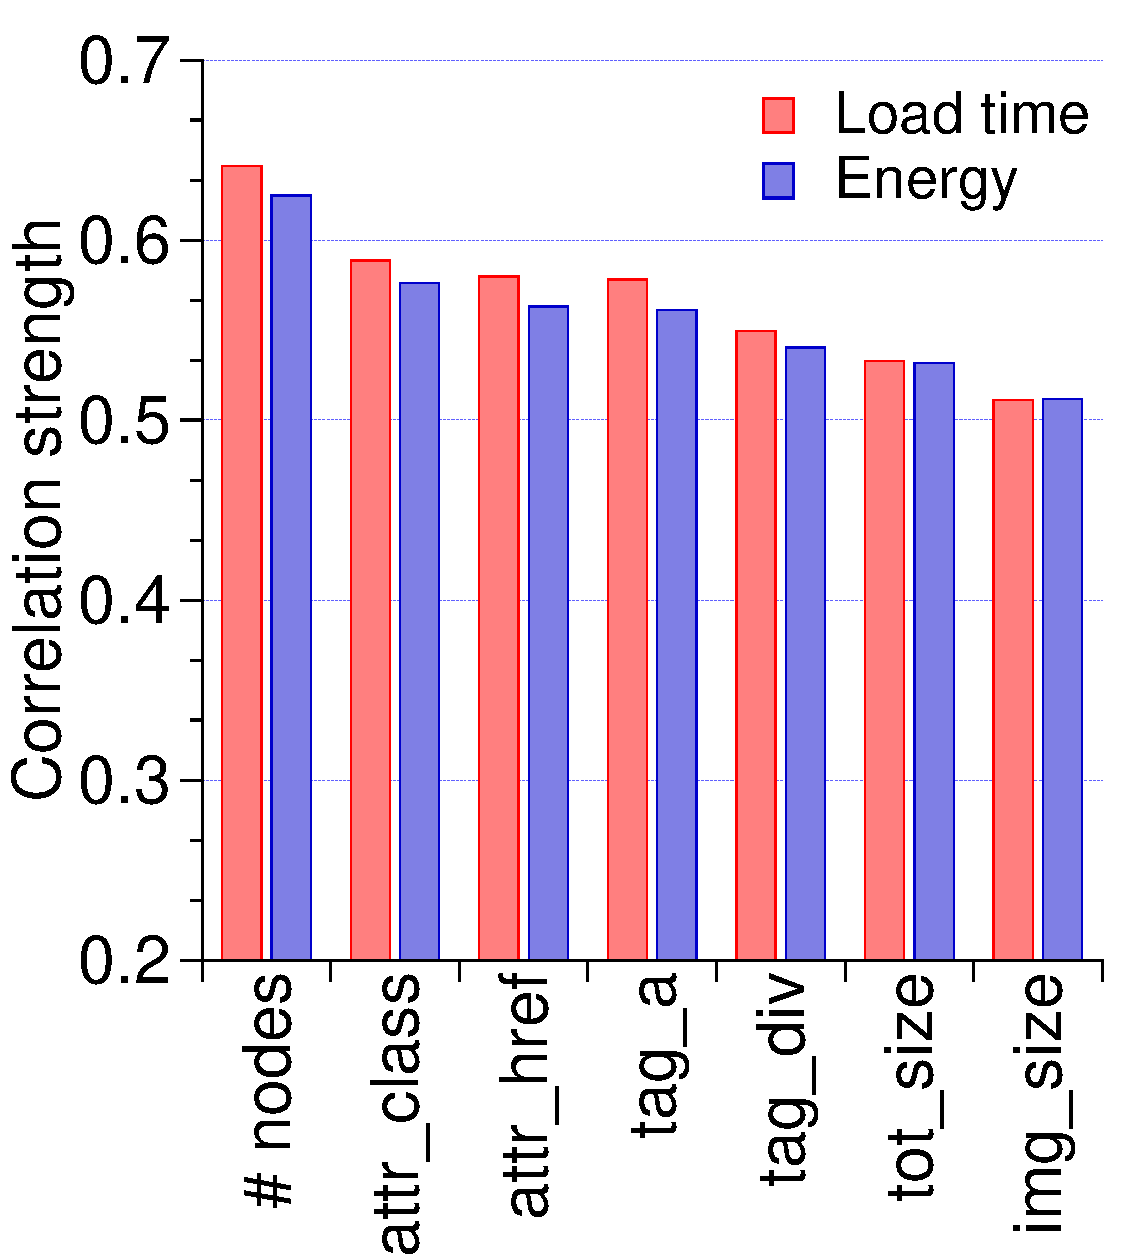
\includegraphics[trim=0 0 0 0, clip, width=.45\columnwidth]{pred-strength-new}
\label{fig:pred-strength}
}
\hspace*{1pt}
\subfloat[Predictor self-correlation.]{
  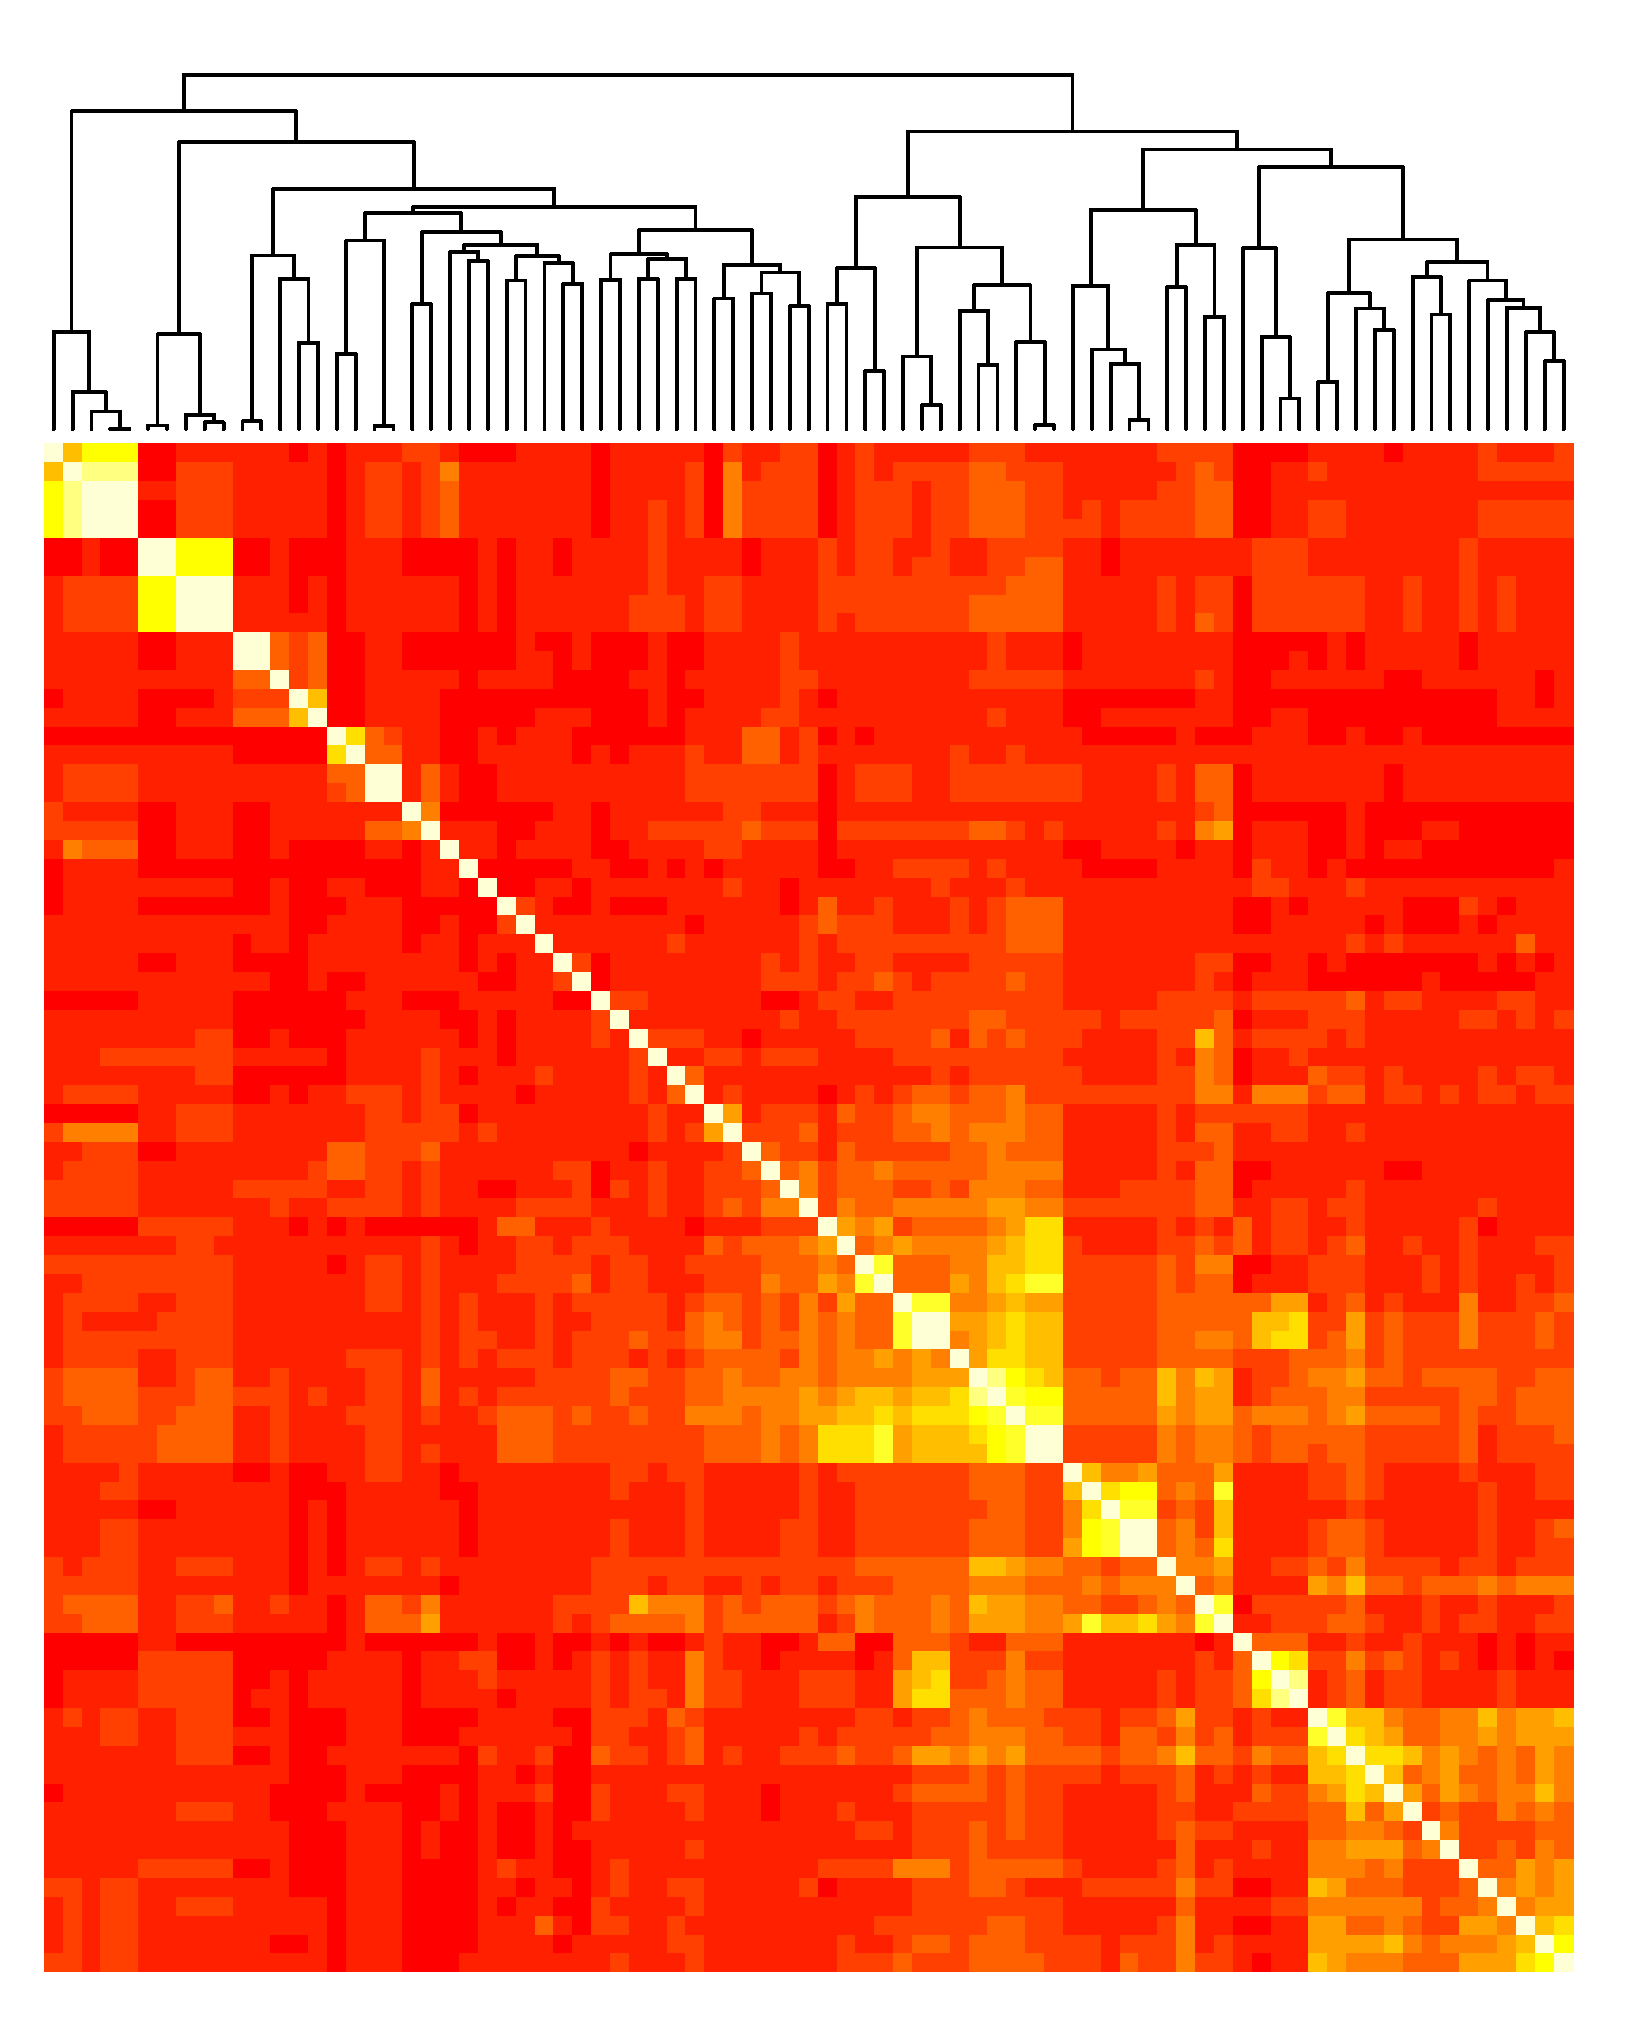
\includegraphics[trim=0 0 0 0, clip, width=.45\columnwidth]{all_cor-new}
\label{fig:all_cor}
} 
\caption{Predictor correlations.}
\label{fig:pred_cor}
\end{figure}

We further minimize overfitting by pruning features that are correlated to each other.  We test the correlation across predictors left after predictor strength test.  The correlation matrix is shown as a heatmap in \Fig{fig:all_cor}. The intensity of a point in the heatmap is proportional to the magnitude of the correlation coefficient between two predictors. The height of the branches in the dendrogram quantifies this magnitude.

In general, we find two types of correlation: inherent correlation and imposed correlation. Several HTML tags and attributes are functionally defined symbiotically and most often used together, exemplifying the inherent correlation. For example, the $<$\texttt{form}$>$ tag describes a form in the webpage, and the \texttt{action} attribute specifies where to submit the form. These two predictors are almost synchronized with each other, suggesting redundancy. Similar examples are the $<$\texttt{a}$>$ tag and the \texttt{href} attributes, which are defined to specify an external hypertext link. Some other predictors do not bear such an inherent relationship, but web developers use them together to describe related information, such as an image's width and height. For example, CSS properties \texttt{height} and \texttt{width} are highly correlated. The descendant selector pattern and class selector pattern also show heavy correlation for this reason.

Furthermore, it is unlikely that the true relationship between the response and all predictors is strictly linear as assumed by simple linear models.  One effective method to model nonlinearity is to fit data with \textit{restricted spline} functions that are piecewise polynomial functions but which force linear fitting beyond the first and last knots~\cite{ESL}.

\subsection{Model Evaluation}
\label{sec:runtime:load:model_eval}

To validate the model, we obtain 2,500 observations in addition to the 2,500 observations used for deriving the model. We incrementally evaluate the effect of various refinement techniques described previously by comparing the accuracy of three regression models. First, we evaluate a basic linear regression (L) model that prunes less-significant predictors. Second, we evaluate linear regression with regularization (R) that further prunes predictors correlated with each other. Third, we evaluate a restricted cubic spline-based (RCS) model using pruned features, which captures the nonlinear relationship between predictors and responses. Of all three models, RCS performs best at predicting both load time and energy. We show all three models for completeness of evaluation.

\paragraph{Performance model} The basic linear regression model (L) has a median and mean error rate of 25.8\% and 32.8\%, respectively, indicating a less-desirable prediction. The regularization-based model (R) reduces the median and mean error rate to 11.5\% and 13.6\%, respectively, due to more aggressive predictor pruning. Restricted cubic spline (RCS) modeling predicts the best, with the median and mean error rate of only 5.7\% and 7.5\% due to its capability of capturing more complex relationships between predictors and responses.

We also assess the distribution or prediction errors. \Fig{fig:perf_cdf} shows the results by presenting the cumulative distribution of the error for three modeling methods. Each ($x$, $y$) point in the graph corresponds to the portion of pages ($y$) that are at or below a particular error rate ($x$). Owing to overfitting, L predicts very accurately for a few webpages, but lacks the capability to be generally applicable to a large range of webpages.  As a result, L can only predict 20.0\% of the webpages within 10\% error. In contrast, R mitigates overfitting due to aggressive pruning, and predicts 44.6\% of the webpages within 10\% error. Finally, RCS further captures the nonlinear relationship, and therefore can predict 73.0\% of the webpages within 10\% error, and 94.0\% webpages within 20\% error.

\paragraph{Energy Model} Similar to the load time model, the RCS-based model performs the best, with the median error rate of 6.4\% (mean of 8.2\%), dropping from the median of 12.3\% and 27.1\% for R and L, respectively. \Fig{fig:energy_cdf} shows the cumulative distribution of the error for three modeling methods. For reasons explained earlier, RCS can predict 70.0\% of the webpages within 10\% error (91.8\% within 20\% error), improving from 41.7\% and 18.7\% of R and L, respectively.

\begin{figure}[t]
\subfloat[Load time model.]{
    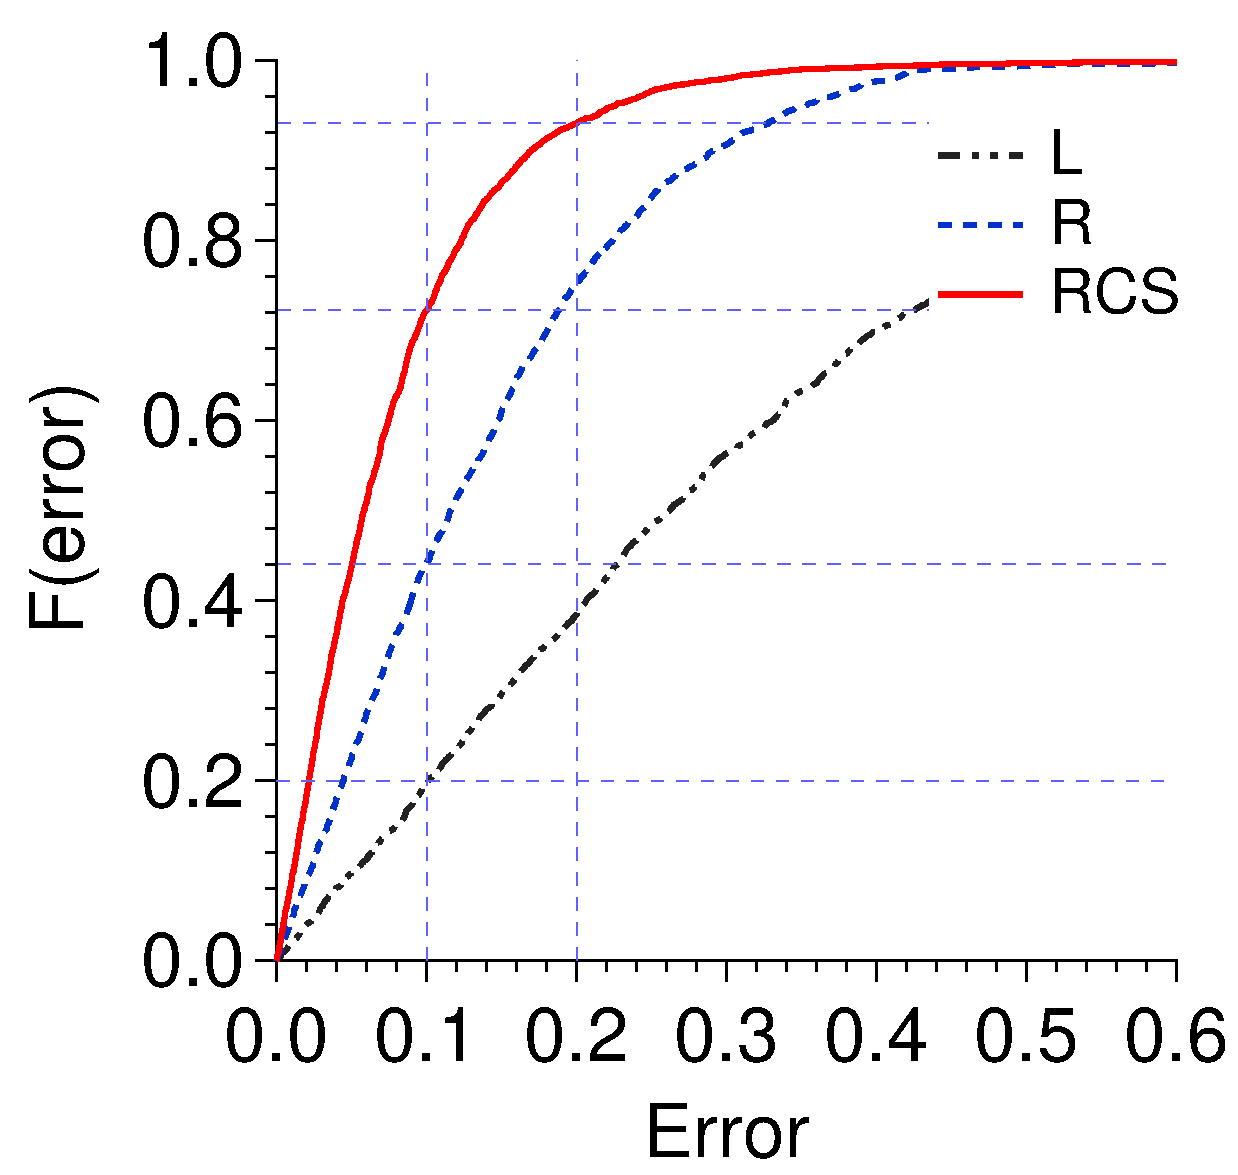
\includegraphics[trim=0 0 0 0, clip, width=.45\columnwidth]{perf_cdf}
\label{fig:perf_cdf}
}
\hspace*{15pt}
\subfloat[Energy model.]{
    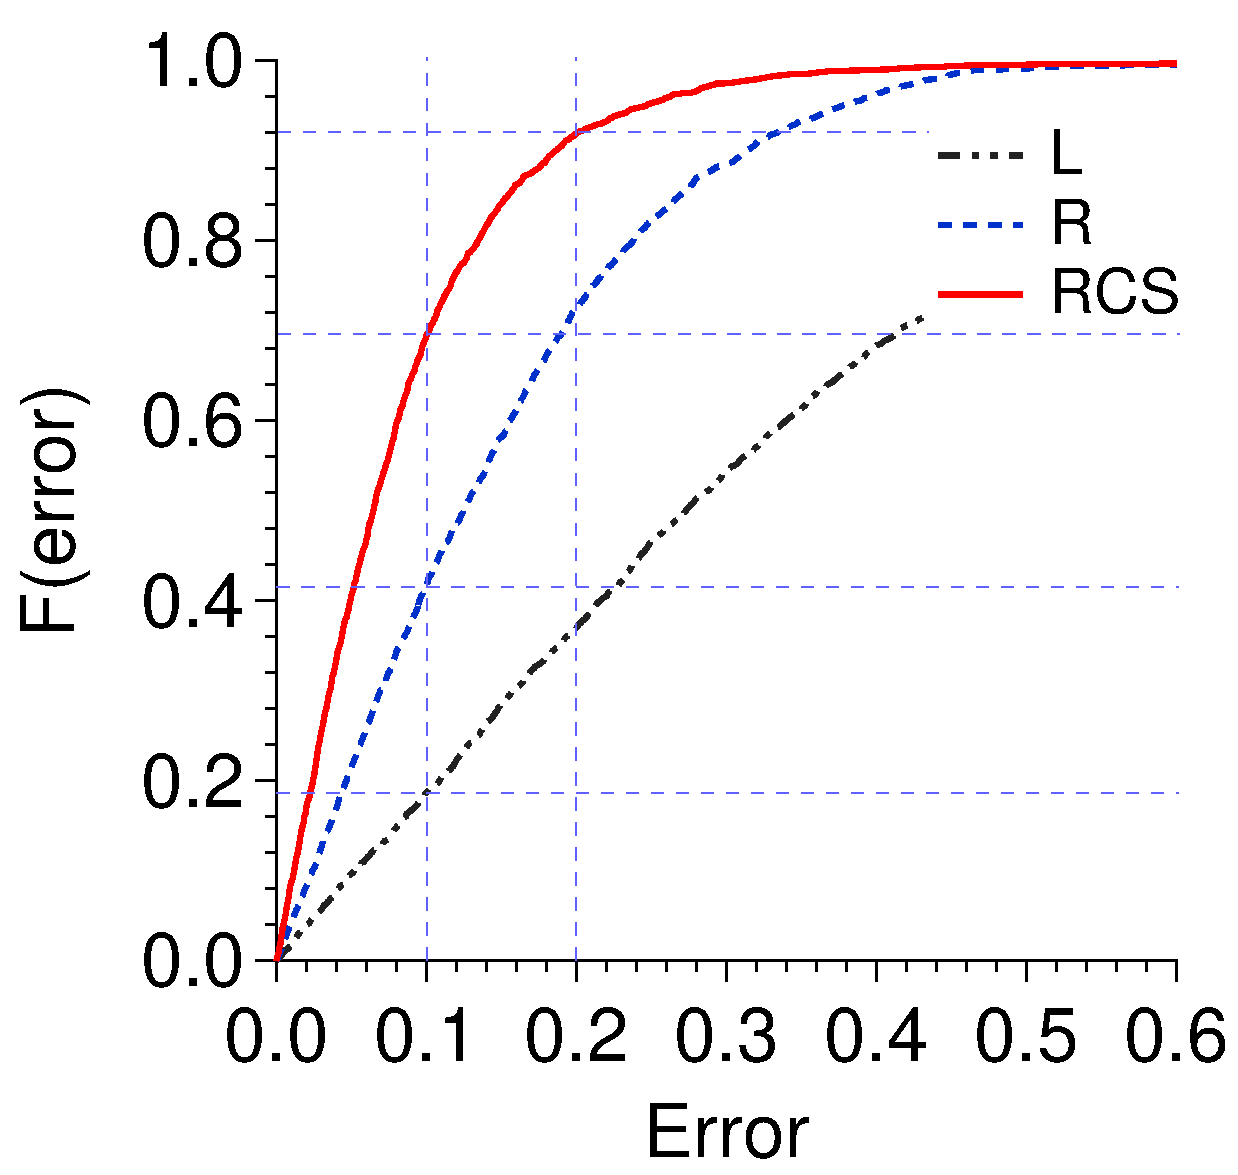
\includegraphics[trim=0 0 0 0, clip, width=.45\columnwidth]{energy_cdf}
\label{fig:energy_cdf}
} 
\caption{CDF of prediction errors.}
\label{fig:model_eval}
\end{figure}

\subsection{Scheduler Implementation}
\label{sec:runtime:load:sched}

\paragraph{Scheduler} During the parsing stage, which takes \textless 1\% of the total execution time, the webpage-aware scheduler extracts webpage characteristics, and feeds them into the prediction models to estimate the webpage load time and energy consumption under different core and frequency configurations.  On the basis of these predictions, the scheduler then identifies the configuration (if possible) that meets the cut-off latency with minimal energy consumption. If no such configuration is found, the webpage is scheduled to the big core with the highest frequency for the best possible performance.

\paragraph{Scheduling Overhead} We consider two major scheduling overheads: prediction and configuration transitioning. Prediction occurs very rapidly (\textless 3~milliseconds on the Cortex-A9 under 1.2~GHz). Moreover, prediction is interleaved with the parsing stage of the rendering engine. As parsing in modern browsers is highly optimized (e.g., asynchronous with the other processing), the prediction overhead is insignificant. On the basis of our measurements, we assume a constant overhead of 5~milliseconds.

Transitioning between hardware configurations involves the penalty of migrating tasks between big/little cores and/or frequency scaling overhead. The major overhead source of task migration is context switch, i.e. (re)storing architecture state such as register files and configuration registers, as well as warming up the private L1/L2 caches (assuming cache coherency between the last-level cache (LLC) of big and little cores). We assume a constant overhead of 20~milliseconds for state (re)storing per context switch, as indicated for the ARM big.LITTLE system~\cite{big.little}. For private cache warmup penalty, prior work shows that performance often improves when private LLCs of big and little cores are powered on together~\cite{PIE}. Thus, we ignore the warmup penalty. Also, prior work suggested that the power overhead of task migration is \textless 0.75\%~\cite{tm}. Thus, we do not consider the additional energy consumption of our scheduling mechanism.

For frequency scaling, we assume 0.3~milliseconds as the overhead. The Linux kernel uses this value on both the Cortex-A9 and A8 systems. This value takes into account both hardware (i.e., voltage regulator module switching frequency) and software overhead (i.e., privilege-level switching overhead for the frequency change request). In our evaluation, since we do not know which configuration the web browser is currently running in, we conservatively consider both the configuration transitioning overhead and the frequency scaling overhead at every scheduling point.

\subsection{Evaluation}
\label{sec:runtime:load:eval}

\begin{figure}[t]
\centering
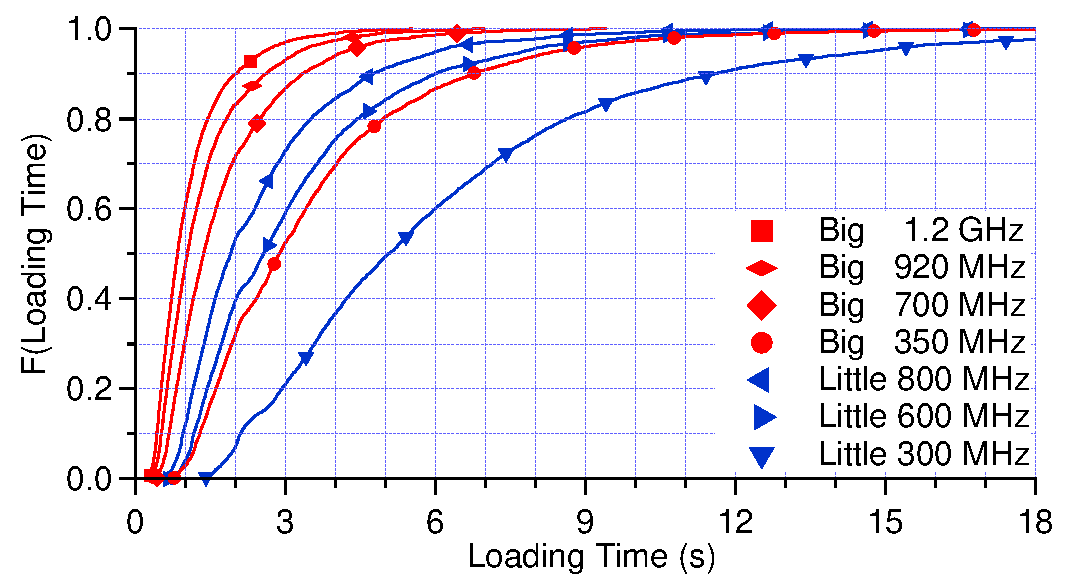
\includegraphics[trim=0 0 0 0, clip, width=.9\columnwidth]{cutoff_cdf}
\caption{CDF of webpage load time under different configurations.}
\label{fig:cutoff_cdf}
\end{figure}

\paragraph{Baseline Mechanism} We compare the webpage-aware scheduling mechanism against an intelligent synthesized OS scheduler that performs on-demand DVFS on a heterogeneous system. The OS scheduler scales the frequency during a webpage load based on simple heuristics of system utilization~\cite{OS_DVFS1,OS_DVFS2}. It samples the CPU usage at a certain period and scales up the frequency if the average CPU usage in the previous sampling period is above a preset threshold, and vice versa. Because no Linux scheduler can yet perform heterogeneous scheduling across big/little cores, we synthesize such a scheduler by running the webpages under the ``on-demand'' cpufreq-governor~\cite{ondemand} on the big core and the little core, individually, and then choose the better result.

We compare the two scheduling techniques with a baseline strategy that consistently yields the best performance. We determine such a baseline by assessing the performance of all the different core and frequency configurations. \Fig{fig:cutoff_cdf} shows the cumulative distribution of webpage load time under each configuration. Each ($x$, $y$) point in the figure represents the portion of webpages ($y$) loaded within a certain delay ($x$). The big core with the peak frequency (1.2~GHz) achieves the best overall performance. It can load 96.5\% of the webpages within 3~seconds. As the frequency and core capability degrade, fewer webpages can be loaded within the same cut-off latency. Therefore, we choose the big core~(A9) with its peak frequency~(1.2~GHz) as the high-performance baseline.

\paragraph{Energy savings} We evaluate the same 2,500 webpages that we used to assess the accuracy of the regression models. Assuming a 3~second cut-off latency, \Fig{fig:results_energy} shows the boxplot of per-webpage energy savings under the webpage-aware and OS schedulers against the high-performance mode. Both schedulers achieve significant energy savings over the high-performance baseline, with a (geometric) average of 83.6\% and 83.0\%, respectively. This is because both schedulers can schedule webpages to the lower power core or lower frequency.

\begin{figure}[t]
\subfloat[Distribution of per webpage energy saving against the baseline.]{
    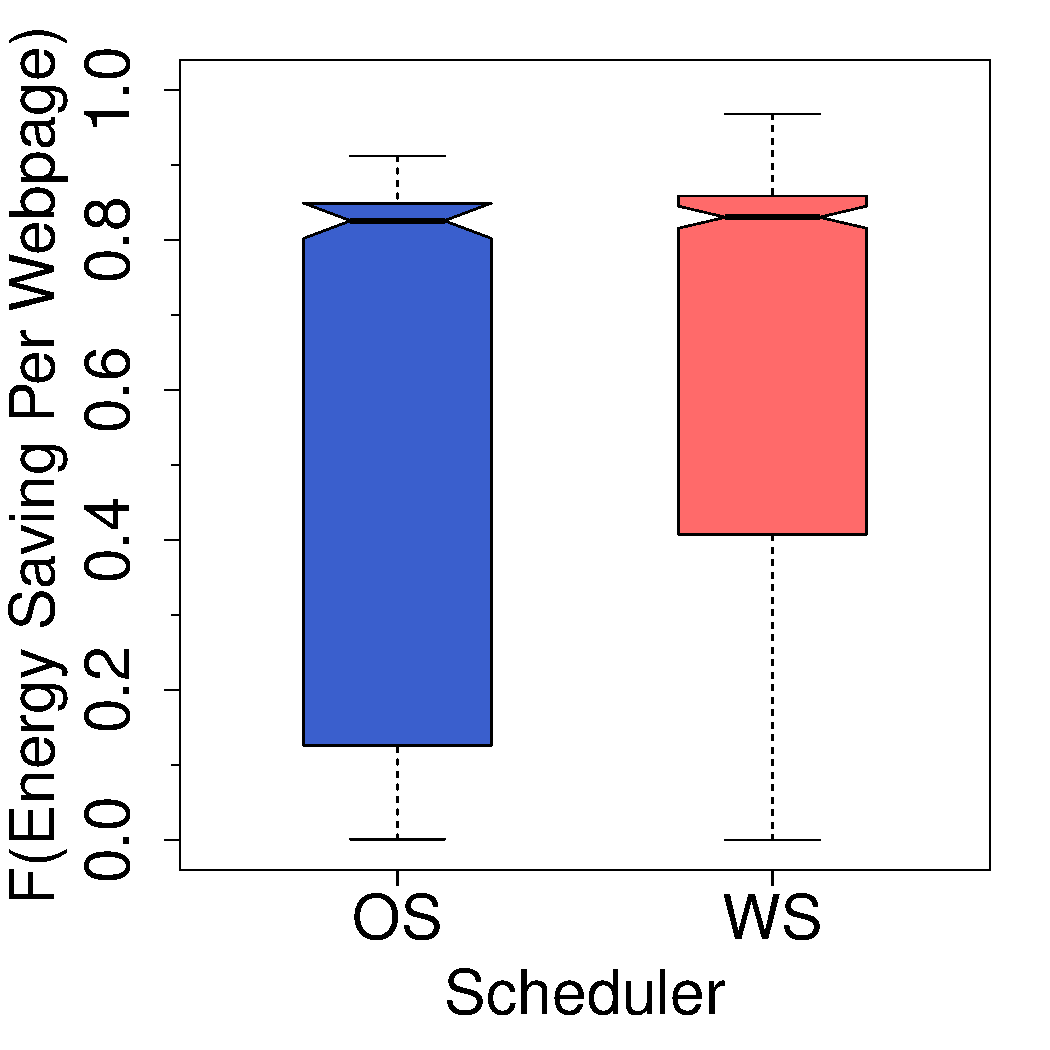
\includegraphics[trim=0 0 0 0, clip, width=.45\columnwidth]{boxplot}
\label{fig:results_energy}
}
\hspace*{15pt}
\subfloat[Number of webpages that load under the strict cut-off latency of 3~seconds.]{
    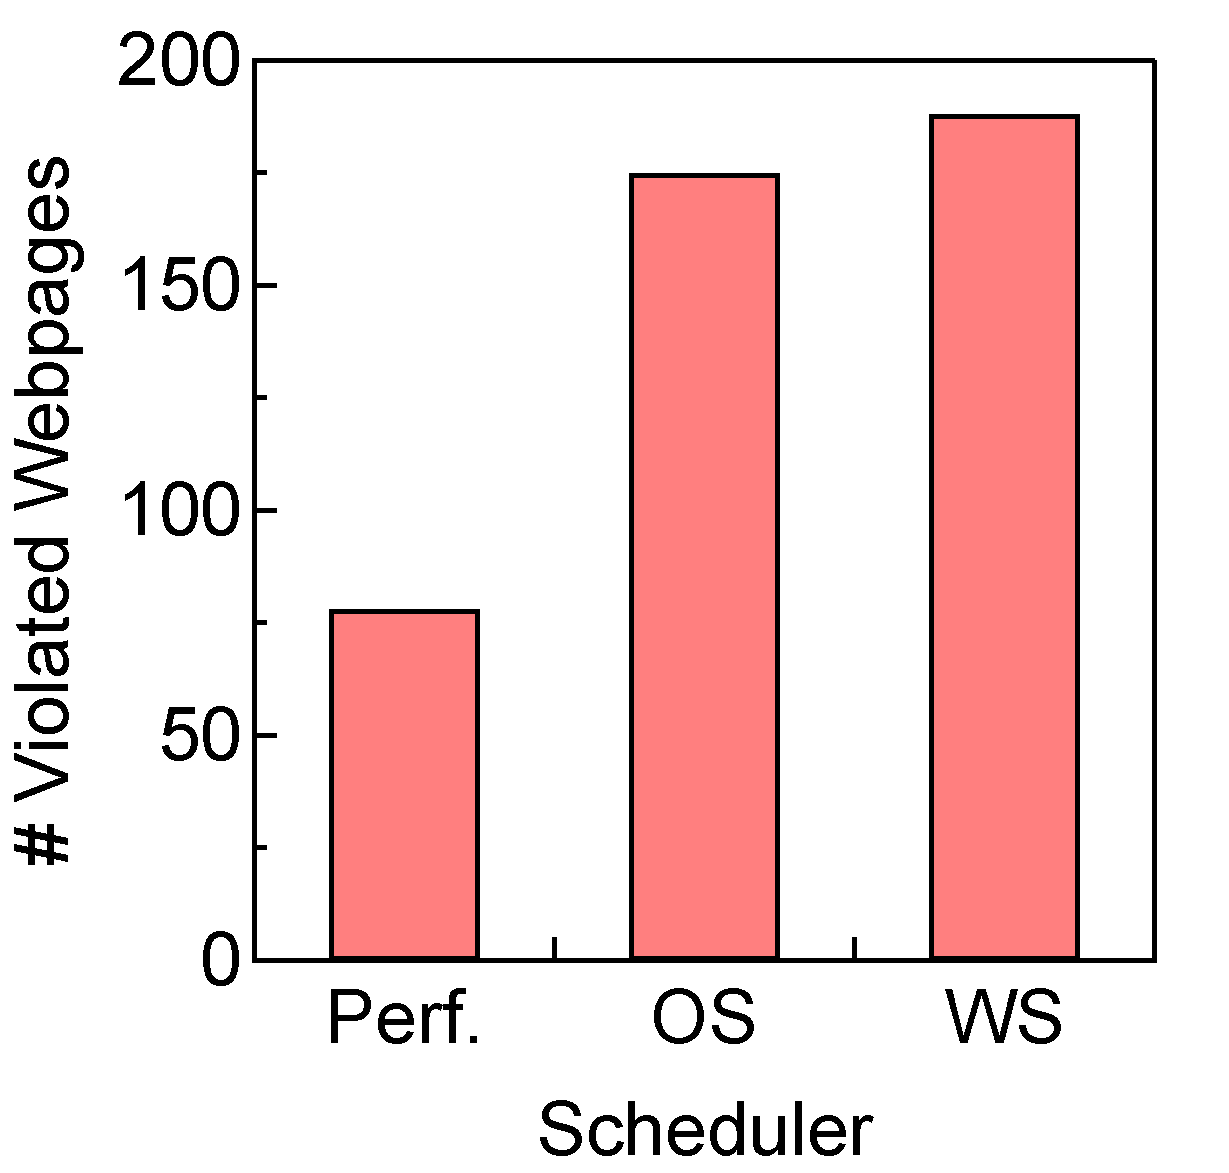
\includegraphics[trim=0 0 0 0, clip, width=.45\columnwidth]{results_cutoff}
\label{fig:results_cutoff}
} 
\caption{Evaluation of different scheduling strategies.}
\label{fig:sched_results}
\end{figure}

The webpage-aware scheduler has a denser energy-saving distribution toward 100\% than the OS scheduler. This indicates that generally the webpage-aware scheduler achieves higher energy savings. \Fig{fig:webpage-aware} shows the histogram of per-webpage relative energy of the webpage-aware scheduler to the OS scheduler. The webpage-aware scheduler saves energy for about 80\% of the webpages. There are several webpages that are mis-scheduled onto the big core that could have met the cut-off latency with the little core. These webpages consume much higher energy under the webpage-aware scheduler than the OS scheduler (\textgreater 2$X$ in~\Fig{fig:webpage-aware}).  On average, the webpage-aware scheduler reduces energy consumption by 8.6\% compared with the OS scheduler.

\paragraph{Performance impact} Both the OS scheduler and the webpage-aware scheduler trade performance for better energy savings compared with the performance mode. We evaluate their behaviors more critically using the number of webpages that violate the cut-off latency under their operations. This data is shown in \Fig{fig:results_cutoff}. The performance mode violates only 3.5\% of the webpages with a 3~second cut-off latency because it always operates at peak computational capability. Both of the software schedulers perform slightly worse. Our mechanism, the webpage-aware scheduler, results in 7.6\% violations, which is only 0.6\% worse than the OS scheduler. However, on (geometric) average, our mechanism loads webpages 4.0\% faster than the OS scheduler.

\paragraph{Cut-off sensitivity} To assess the webpage-aware scheduler under variable user demands and mobile device conditions, we also experiment with different cut-off latencies. For example, when the end user requests faster webpage load at 2~seconds, the mechanism achieves 7.3\% energy savings over the OS scheduler while violating 4\% fewer webpages. In a battery conservation mode where performance is less critical and the cut-off latency is relaxed to 10~seconds, the webpage-aware scheduler achieves 11.8\% energy savings compared with the OS scheduler while exceeding the cut-off latency for only 0.02\% webpages in total. We conclude that the webpage-aware scheduler is flexible to changing user requirements.

\paragraph{Prediction Accuracy} Scheduling effectiveness relies on the load time and energy prediction accuracy. We study the impact of the prediction accuracy by comparing webpage-aware scheduling with an Oracle scheduler that assumes perfect prediction under the 3~second cut-off latency. There are two types of misprediction: over-prediction causes webpages to load on a more powerful configuration that consumes more energy than the ideal one but does not cause cut-off violation; under-prediction loads webpages on a weaker configuration that consumes less energy but violates the cut-off constraint.  Our models lead to 10\% over-prediction and 4.1\% under-prediction. Compared with the Oracle scheduler, the webpage-aware scheduler results in 4.1\% cut-off violation but ``conserves'' 9.7\% energy.

\paragraph{Analysis} The advantage of the webpage-aware scheduler lies in its awareness of the webpages characteristics and the cut-off latency. As a result, it predicts and chooses a proper, albeit fixed, configuration for each webpage. In contrast, the OS scheduler's DVFS decision is based on the system utilization, which has no direct correlation with the webpage characteristics/cut-off latency and is sensitive to other system activities. Therefore, it may lead to a suboptimal performance-energy trade-off or even miss the cut-off constraint.

For example, when loading \website{www.newegg.com} (top-right in~\Fig{fig:pareto}) under the OS scheduler, we find that the CPU usage on the big core reaches above 95\% for around 40\% of the time and (unnecessarily) incurs peak frequency (i.e. 1.2~GHz).  When in fact, the big core with 720~MHz chosen by the webpage-aware scheduler is sufficient  to meet the 3-second cut-off latency, achieving 20\% energy savings compared with the OS scheduler in our experiments.

However, the flexibility to scale the frequency while loading a webpage sometimes allows the OS scheduler to exploit the marginal value of energy, i.e. a slight increase in energy (through frequency scaling) can bring the webpage back within the cut-off latency that would have been missed if the webpage were loaded using a lower frequency.

For example, \website{www.autoblog.com} (top-left in~\Fig{fig:pareto}) when loaded under 920~MHz (on the big core) just surpasses the 3-second deadline by 0.1 seconds, but has to fall back using 1.2~GHz under the webpage-aware scheduler. At 1.2~GHz, the webpage loads in only 1.8 seconds but consumes 37\% more energy than 920~MHz. However, under the OS scheduler, our statistics show that the OS boosts the frequency above 920~MHz for only around 20\% of the time, and finishes the load in 2.7 seconds. Compared with the webpage-aware scheduler that runs at 1.2~GHz for this webpage, the OS scheduler in this case saves 20\% energy, effectively exploiting the high marginal value of energy.

\paragraph{Integrated Scheduler} For complete evaluation, we also assess an integrated scheduler that combines the webpage-aware scheduler with OS DVFS. The purpose is to exploit the potentially high marginal value of energy via OS DVFS, but bound the DVFS space to avoid frequencies that are unnecessarily high (wasting energy) or low (missing the cut-off latency).

\begin{figure}[t]
\subfloat[Relative energy of the webpage-aware scheduler against the OS scheduler.]{
  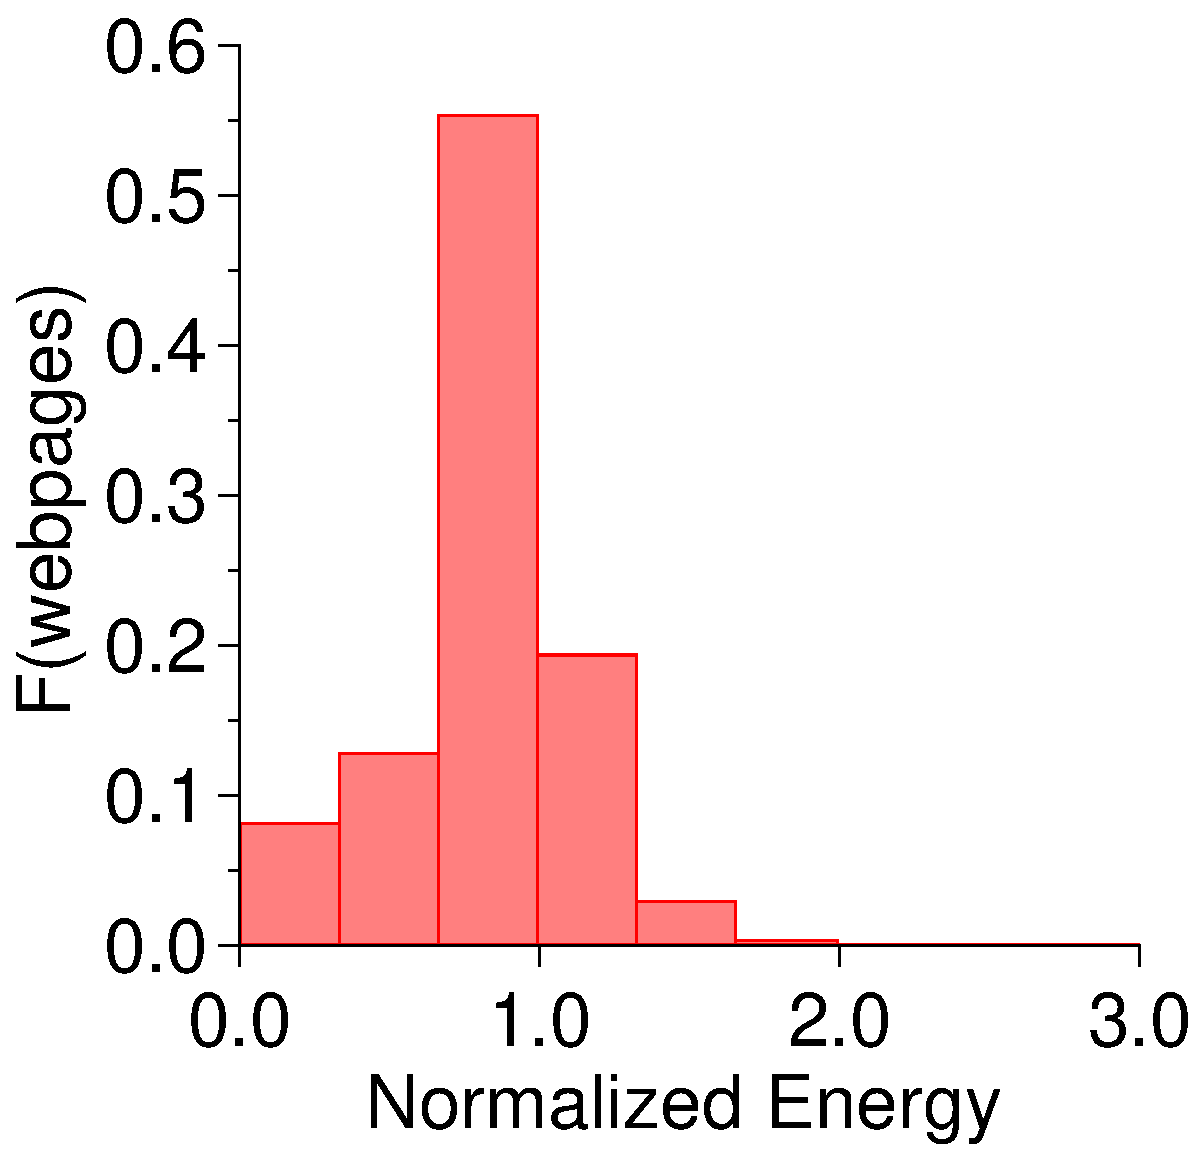
\includegraphics[trim=0 0 0 0, clip, width=.45\columnwidth]{webpage-aware}
\label{fig:webpage-aware}
}
\hspace*{15pt}
\subfloat[Relative energy of the integrated scheduler against the webpage-aware scheduler.]{
  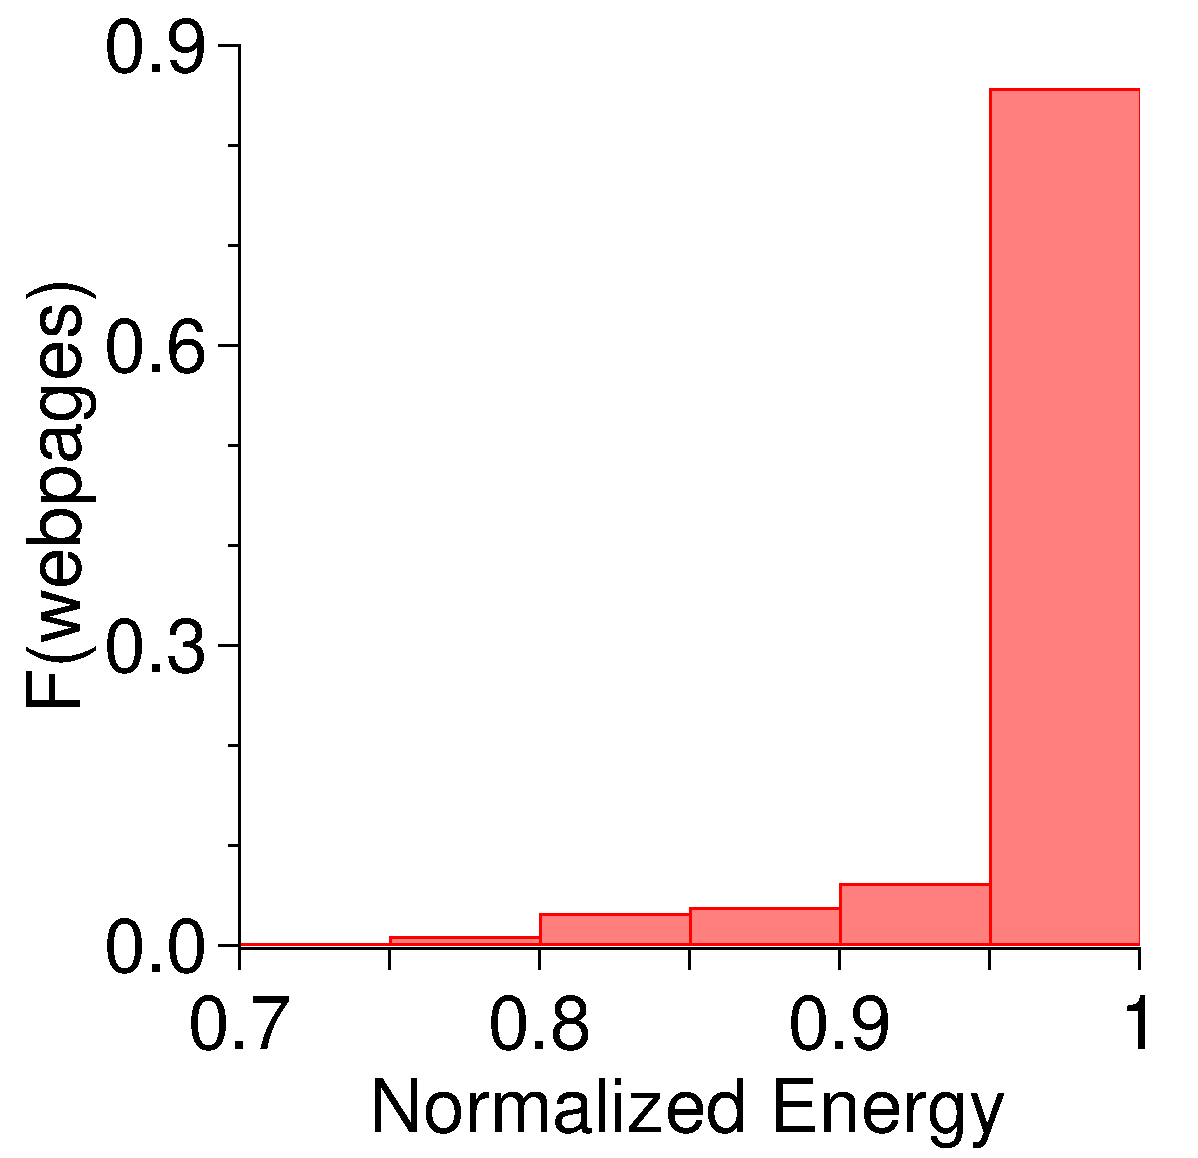
\includegraphics[trim=0 0 0 0, clip, width=.45\columnwidth]{integrated}
\label{fig:integrated}
} 
\caption{Distribution of per-webpage energy comparisons.}
\label{fig:e_saving}
\end{figure}

Specifically, the webpage-aware scheduler first restricts the OS DVFS scheduling space to two frequencies: a lower frequency that just meets the cut-off constraint and a upper frequency that just misses the constraint. Given the two frequencies, the webpage-aware scheduler tries to ensure that the cut-off latency can still be met by further tuning the percentage of time spent in either frequency. In practice, we set the \textsf{scaling\_max\_freq} and \textsf{scaling\_min\_freq} of the Linux cpufreq-governor to the lower and upper frequency, respectively. We set the \textsf{up\_threshold} to control when to promote to the higher frequency~\cite{ondemand}. For example, for \website{www.autoblog.com} (top-left in~\Fig{fig:pareto}), the OS DVFS on the big core would only operate on 1.2~GHz and 920~MHz. Because 920~MHz is nearly able to hit the deadline, only a small portion of the webpage load must be run in the upper frequency.  

\Fig{fig:integrated} shows, under a 3 seconds cut-off constraints, the histogram of per webpage relative energy of the integrated scheduler to the webpage-aware scheduler.  The integrated scheduler consistently out-performs the webpage-aware scheduler with 3.0\% average energy savings (up to 30\%).  We leave the full integration and detailed comparison for future work.

\section{Event-based Scheduling}
\label{sec:runtime:ebs}

I propose event-based scheduling (EBS) as the mechanism to optimize energy-efficiency for the Touching (T) and Moving (M) interactions. Each T or M interaction is internally translated to an application event. EBS is based on the observation that a T or M event may occur repetitively throughout a Web application usage session such that it is possible to predict the ideal architecture configuration of an event based on its history information of performance and energy consumption. We first present our motivation for performing event-based scheduling at the event handler level (\Sect{sec:runtime:ebs:char}). We then provide a high-level design overview of the event-based scheduling framework~(\Sect{sec:runtime:ebs:overview}) and then describe its implementation details~(\Sect{sec:runtime:ebs:sched}).

\subsection{Scheduling Unit}
\label{sec:runtime:ebs:char}

\begin{figure}[t]
\centering
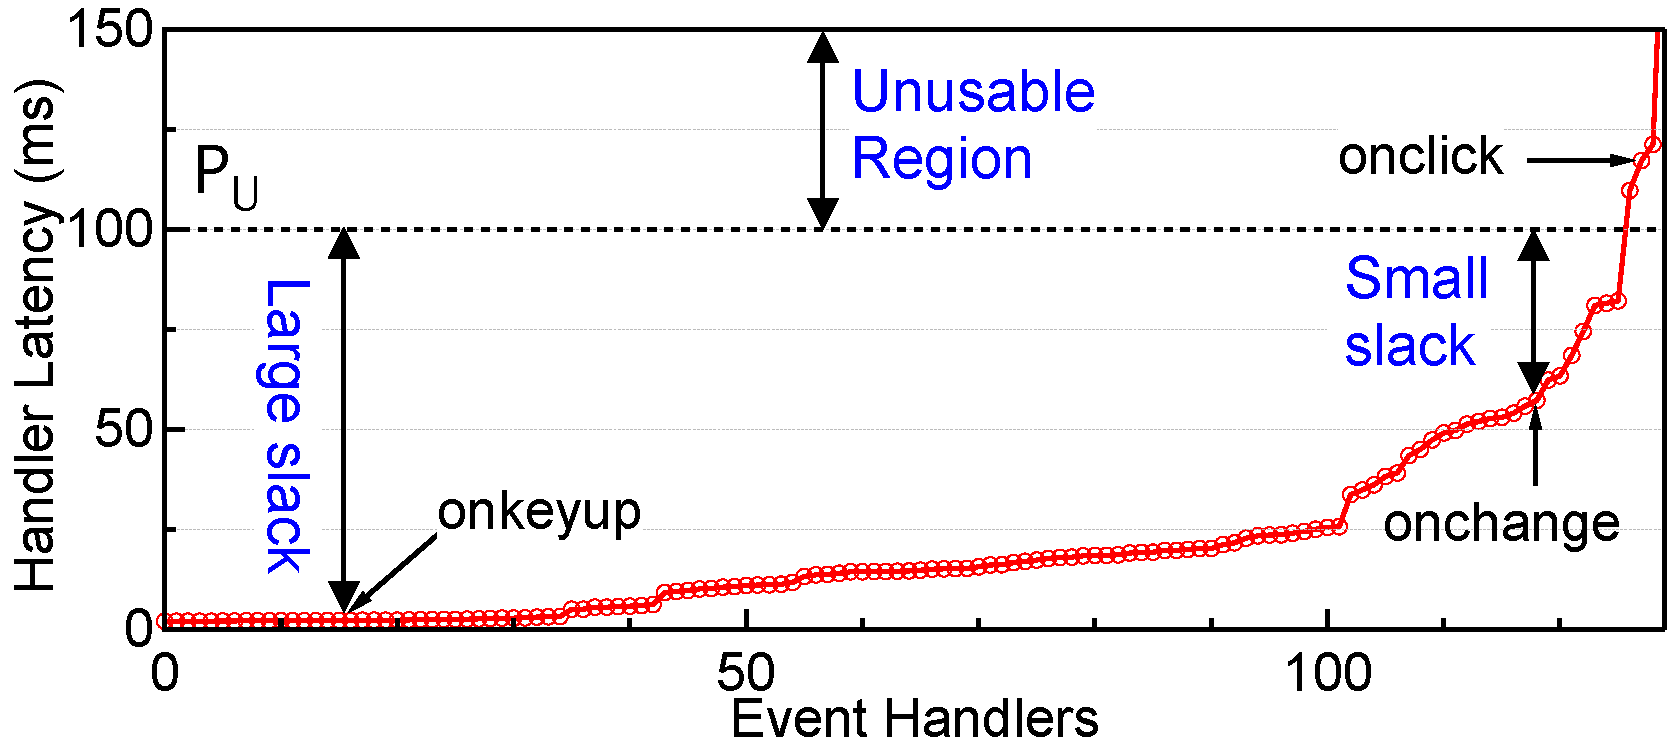
\includegraphics[trim=0 0 0 0, clip, width=0.9\columnwidth]{slack}
\caption{Event handler variation in Ember.js todo list application.}
\label{fig:slack}
\end{figure}

The scheduling unit in the event-based scheduler is the event handler. Whenever an event is triggered, a corresponding event handler is executed. \Fig{fig:runtime} provides an example, showing how event handlers H1, H2, and H3 (in that order) are pushed into the event queue for execution. For events that share the same performance constriant, we find that their event handlers have different execution latencies, and therefore lead to different performance slacks. We must treat each event handler differently and make scheduling decisions at that granularity.

We explain the variation in the event handlers' execution behavior using the Ember.js-based todo list application. \Fig{fig:slack} shows the sorted execution latencies of all the event handlers. The $x$-axis corresponds to the event handlers and the $y$-axis corresponds to the event handlers' execution latencies. In this example, we assume that the performance target for the scheduler is 100~ms, which is a common performance target for a smooth responsiveness.

We observe a large latency variation for the handlers in~\Fig{fig:slack}. We label three of the application's representative event handlers as the application executes: \texttt{onkeyup},~\texttt{onchange}, and~\texttt{onclick}. The~\texttt{keyup} event handler only processes one keystroke and therefore finishes execution very quickly in just 2~ms, which leaves a large amount of slack (98\%) for the scheduler to exploit. In contrast, the~\texttt{onchange} event handler adds one entry into the todo list. It requires about 50~ms for execution, which translates to only about 50\% slack in performance. Lastly, the~\texttt{onclick} event handler deletes all the entries in the todo list. The processing time exceeds the performance constraint, and as such there is no opportunity to exploit performance slack. Instead, it requires a higher performance configuration, if available.

\subsection{Scheduler Design Overview}
\label{sec:runtime:ebs:overview}

The event-based scheduler predicts the ideal heterogeneous architecture execution configuration (i.e., a $\langle core, frequency \rangle$ tuple) whenever an event is triggered and the corresponding event handler is executed such that it ``barely'' meets the performance target with minimal energy consumption. It is important to emphasize that one event may lead to multiple frames being updated. Therefore, the \ebs runtime operates on a per-frame basis as frames are what ultimately dictate user perceivable experience. If an event execution only produces one frame, the runtime finds the ideal execution configuration for the single frame associated with the event. If an event's execution leads to a sequence of frames such as in an animation, the runtime continuously identifies the ideal execution configuration for each frame until all the frames associated with the event are produced. All the associated frames share the same QoS target of the event.

The key idea of identifying an event's ideal execution configuration is to build a performance model and an energy model. They predict an event's latency and energy consumption under any core and frequency combination. With the two models, EBS sweeps all possible core and frequency combinations and selects the one that meets the QoS target with minimal energy.

\begin{figure}[t]
\centering
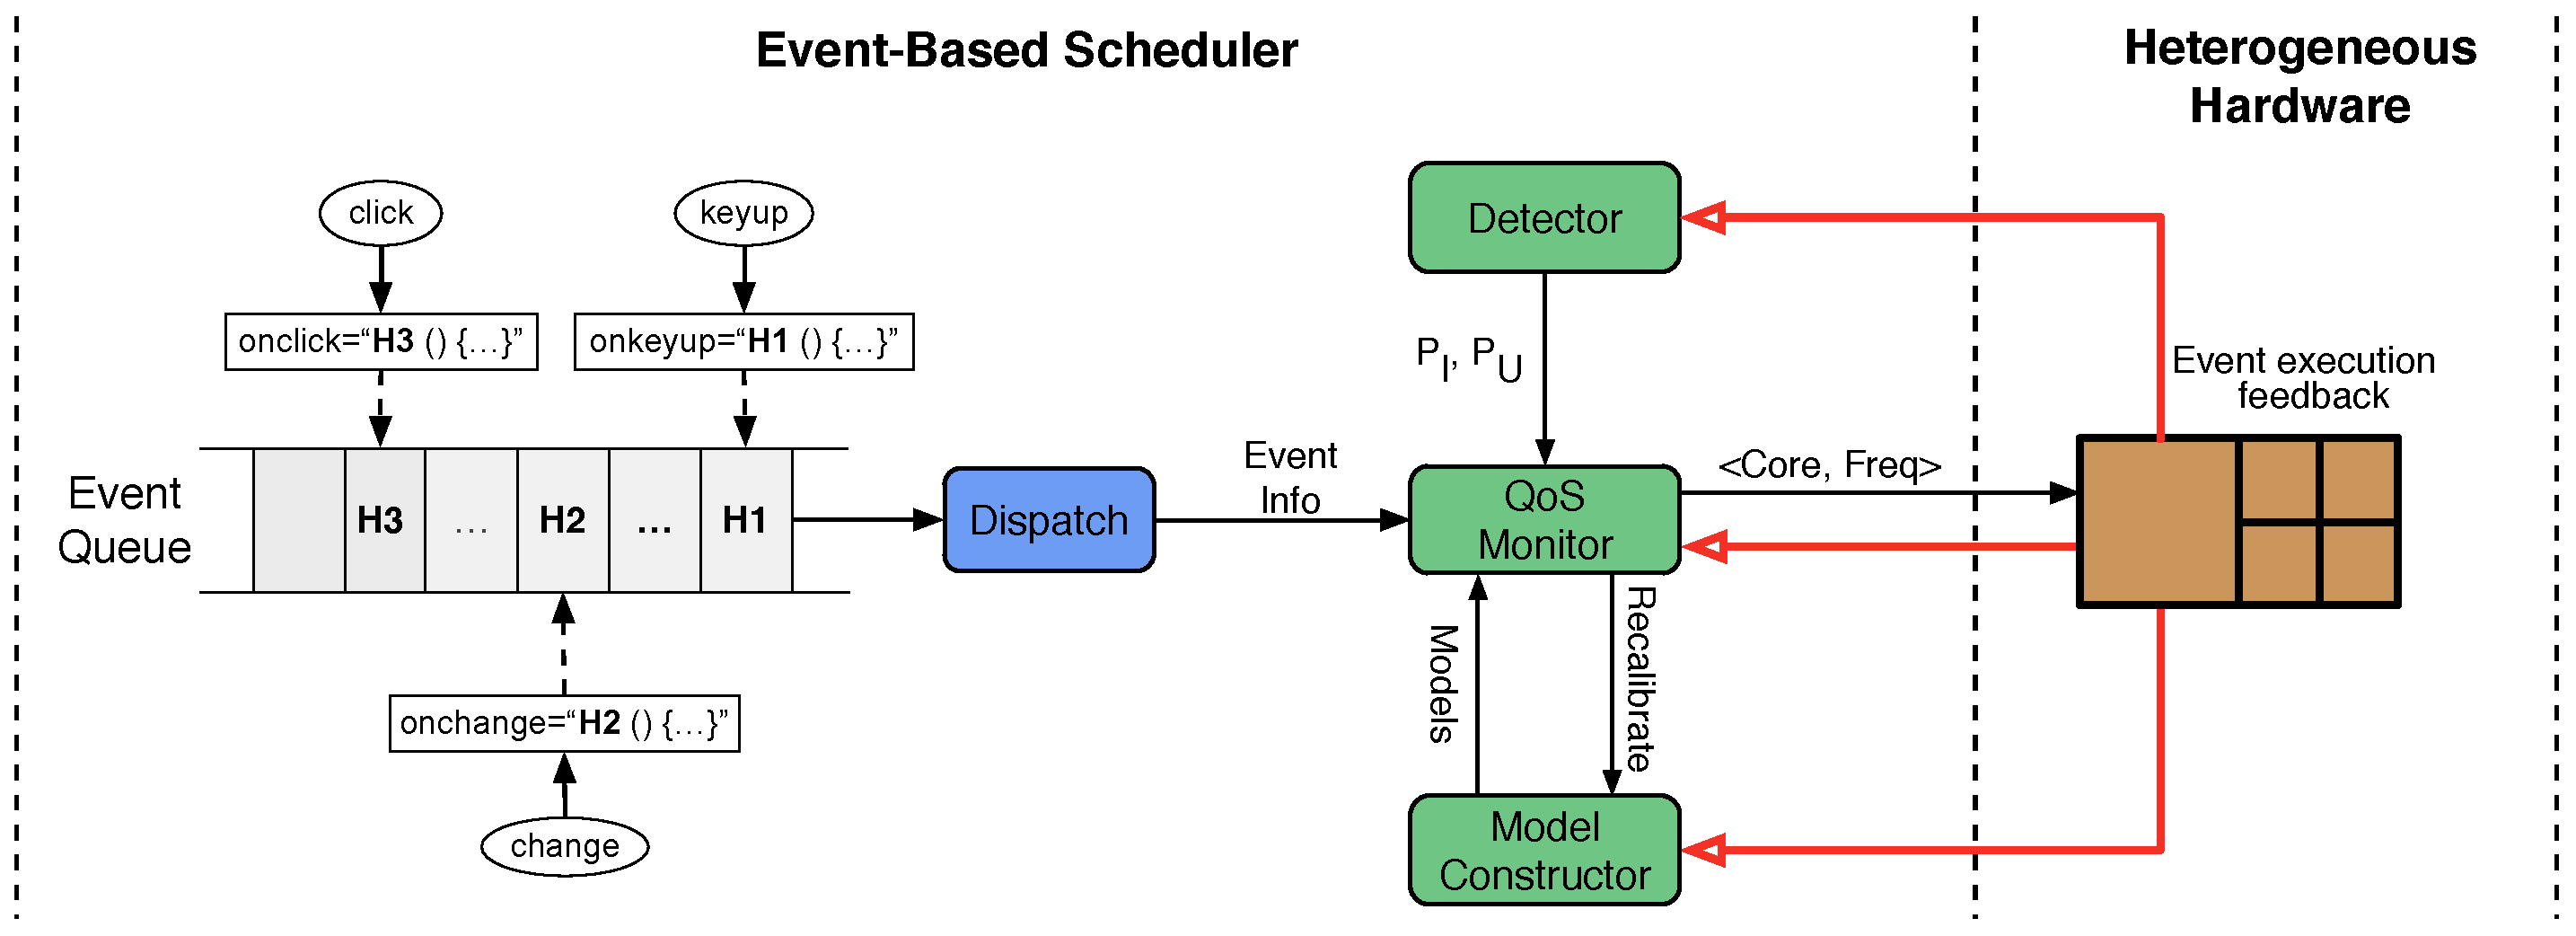
\includegraphics[trim=0 0 0 0, clip, width=\columnwidth]{runtime}
\caption{Event-based runtime scheduling framework.}
\label{fig:runtime}
\end{figure}

The scheduler consists of a simple dispatch frontend and scheduling backend as illustrated in~\Fig{fig:runtime}. The frontend \textit{Dispatch} unit extracts relevant event information, and passes it to the backend. The backend consists of a \textit{Detector}, a \textit{Model Constructor} and a \textit{QoS Monitor}. The detector automatically identifies each event's QoS requirement. In its simplest form, the detector assumes a default latency target, such as 100~ms, for each event. If an event is annotated with programmer-guided QoS hints such as those enabled by the \greenweb language extensions as I will discuss in \Sect{sec:lang}, the detector can also extract the specified QoS information from the application. The model constructor builds a performance and energy model for each event. The models and event QoS information are then fed into the QoS monitor, which predicts the architecture configuration for executing an event while meeting the specified QoS target.

During application execution, the QoS monitor keeps monitoring event execution time and energy consumption on the hardware and uses the information to adjust its prediction and scheduling decisions on the fly, similar to conventional feedback-driven optimizations~\cite{FDO}. We will explain the detailed operation of the monitor in the next subsection. Intuitively, it is possible for the performance and energy models to underpredict or overpredict the architecture configuration. Under such circumstances, the monitor can decide to tune the predicted frequency or transition between big and little cores. If the models are deemed completely unusable, the monitor informs the model constructor to recalibrate the models. We now describe some key implementation details of the QoS monitor operations.

\subsection{Scheduler Implementation Details}
\label{sec:runtime:ebs:sched}

\paragraph{Performance Model} We construct performance models for big and little cores separately. Each model predicts the event handler execution latency under different frequencies. We use the classical DVFS analytical model initially proposed in~\cite{dvfs_model}, and employed in subsequent work, such as~\cite{dvfs_power}:
\begin{align*}
Execution\,\,\,time = T_{memory} + N_{dependent}/f
\end{align*}
where $f$ is the CPU frequency, $T_{memory}$ is the absolute memory access time that does not change with respect to the CPU frequency, and $N_{dependent}$ is the number of CPU cycles that are not overlapped with the memory accesses.

Strictly speaking, $N_{dependent}$ is a function of $f$. However, precisely constructing a model that varies $N_{dependent}$ with $f$ is complex and introduces a large calibration overhead at runtime. In our experiments, we find that it is feasible and necessary to trade model precision for performance. In particular, we find that treating $N_{dependent}$ as a constant is sufficient in our case.

Given this simplification, the model constructor builds the model with the event latency under two different frequencies by calculating the value of $T_{memory}$ and $N_{dependent}$. The trade-off in choosing the two frequencies is that on one hand using two sufficiently different frequencies provides higher accuracy, since the execution latencies from closer frequencies are more susceptible to measurement noise. But on the other hand, using two frequencies that are extremely high and low may result in execution falling in the  imperceptible or unusable QoS regions, ultimately wasting energy. In our current implementation, we use the highest and the second-highest frequencies to construct the performance model. We find that the run-to-run variation for the data collected using these two frequencies is low, resulting in a robust model.

\begin{figure}[t]
  \centering
  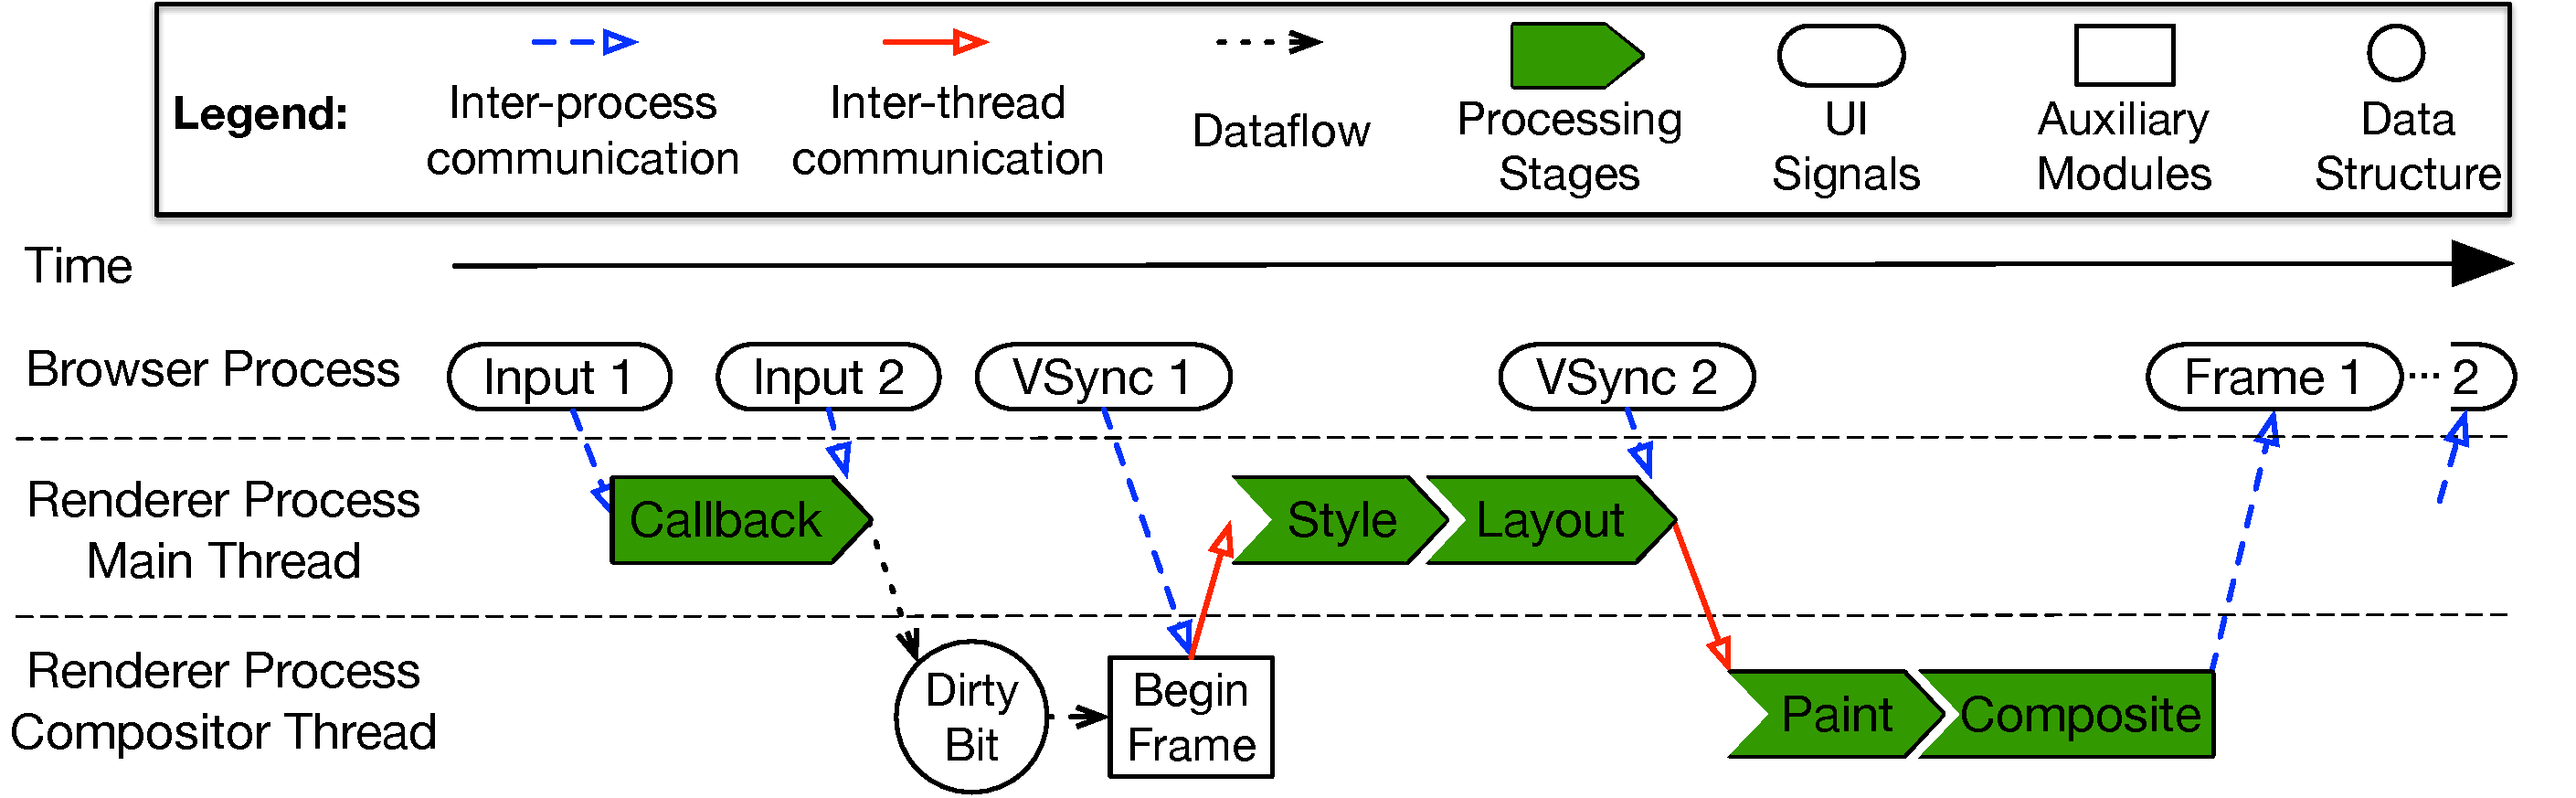
\includegraphics[trim=0 0 0 0, clip, width=\columnwidth]{inputs}
  \caption{The simplified view of frame lifetime in modern multiprocess/thread browsers. A frame starts when the browser process receives an input event and ends when the frame is displayed and the browser process is signaled. In between, an input event is processed by different stages spread across multiple threads. Different input events might interleave with each other.}
  \label{fig:inputs}
\end{figure}

\paragraph{Frame Latency Tracking} Tracking frame latency is crucial to constructing the performance and energy model. However, accurate frame latency tracking is a nontrivial task, primarily because of the complexities involved in generating a frame in modern Web browsers. Most prior work either is concerned only with the callback latency~\cite{ebs,efetch}, which, as we will show later, contributes to only a portion of frame latency, or it considers logical latency (e.g., the number of conditionals evaluated), which is insufficient to construct the prediction models~\cite{eventbreak}.

Accurately tracking frame latency requires us to understand how a frame is processed internally by a Web browser. Using Google Chrome browser as an example, \Fig{fig:inputs} illustrates a typical frame lifetime, starting from when an input event is received by the browser to when the frame is generated. Although we focus on Chrome, the execution model is generally applicable to almost all modern Web browsers such as Firefox, Safari, Opera, and Internet Explorer.

The browser process receives an input event and sends it to the renderer process, which applies five processing stages to produce a frame: callback execution, style resolution, layout, paint, and composite~\cite{renderingpipeline}. In the end, the browser process receives a signal indicating that the frame is produced. To improve performance, the processing stages are spread across two threads, and some portion of the composite stage could be offloaded to GPU (not shown). Note that our performance model in \Equ{eq:dvfs} captures the GPU processing time.

The key to latency tracking is to accurately attribute a frame to its triggering input. Two complexities of the frame generation process make frame attribution non-trivial. First, different input events might be interleaved. For the example in \Fig{fig:inputs}, Input 2 is triggered before Input 1 finishes. Naively associating an input event with its immediate next frame in this case would mistakenly attribute Frame 1 to Input 2.

Second, one frame might be associated with multiple input events. This is because modern browsers generate a new frame only when the display refreshes, i.e., a VSync signal arrives (typically 60~Hz on a mobile device), to avoid screen tearing~\cite{jankbusting,vsync}. If multiple callback functions have been executed before a VSync arrives, their effects are batched and cause only one frame. The batching is achieved through a \textit{dirty bit}. Each callback sets a dirty bit to indicate whether a new frame is needed as a result of callback execution. Callbacks from different inputs write to the same bit, but as long as one callback sets the dirty bit, a new frame will be generated when the browser later receives a VSync signal.

\begin{figure}[t]
  \centering
  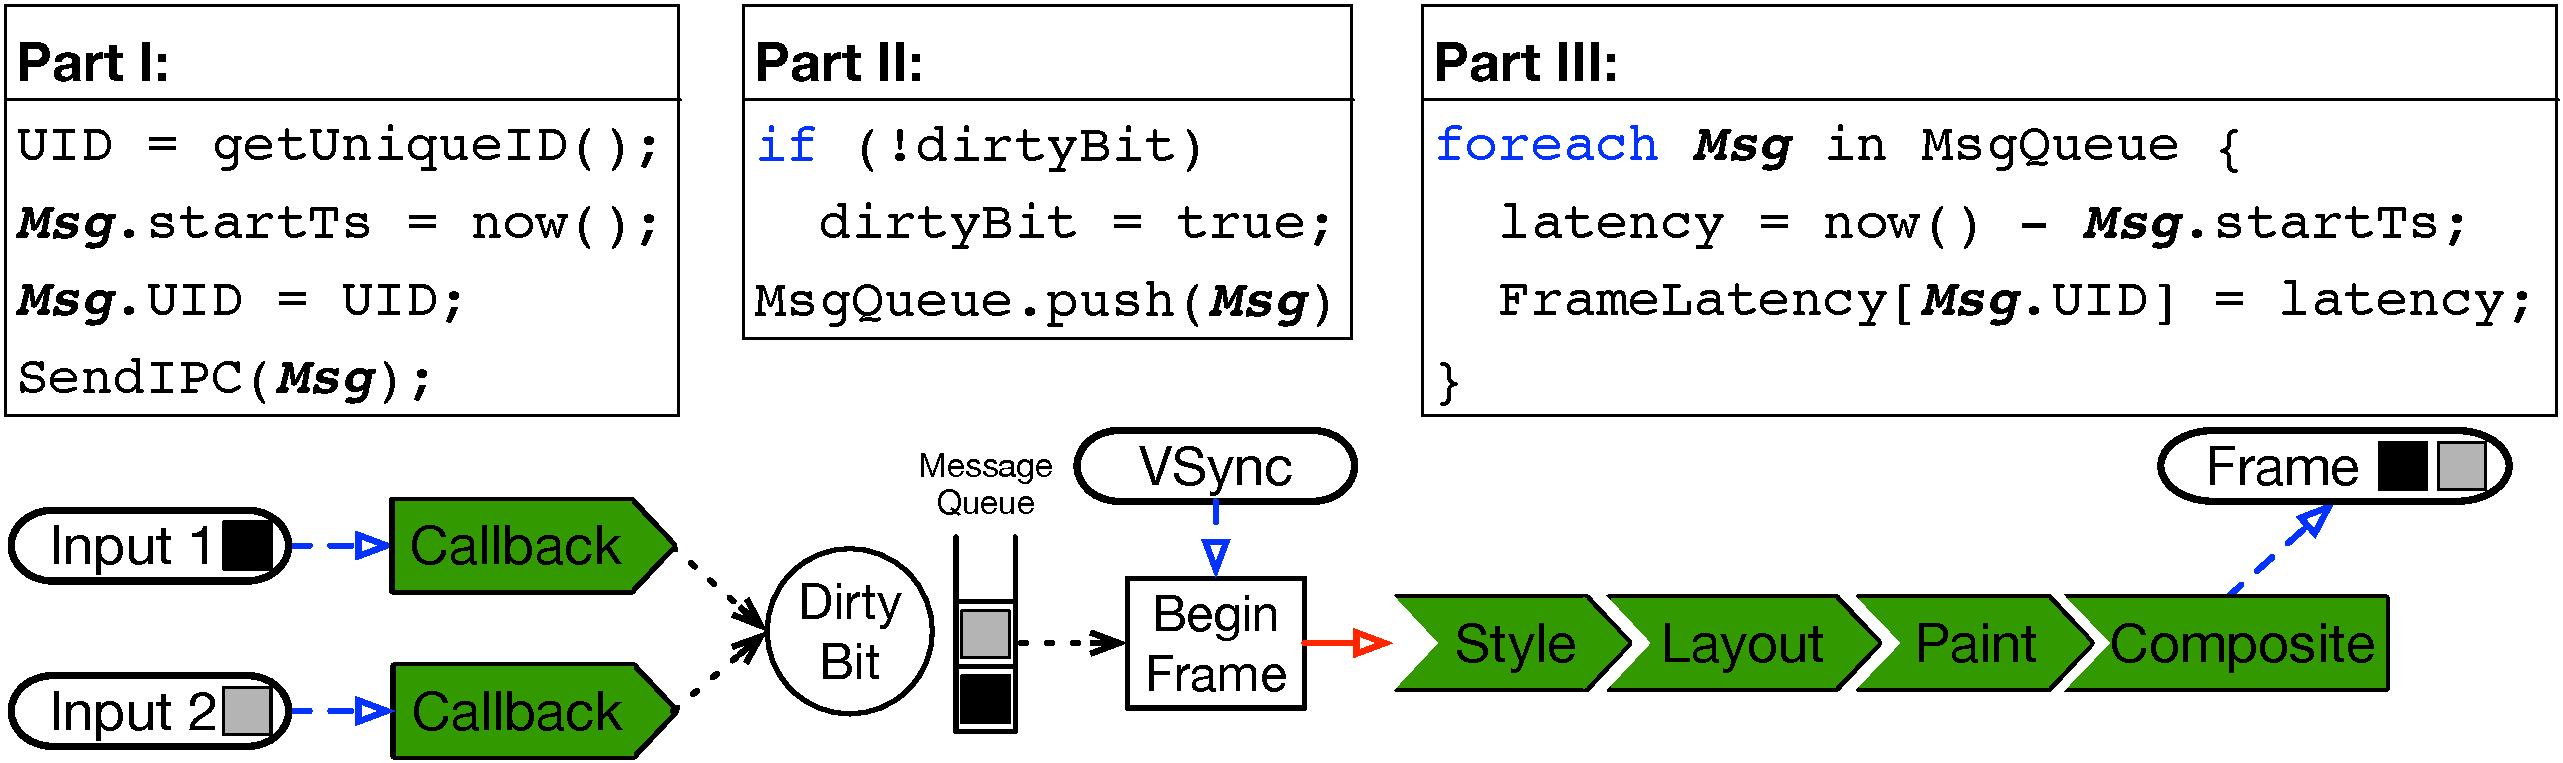
\includegraphics[trim=0 0 0 0, clip, width=\columnwidth]{tracking}
  \caption{Frame tracking algorithm. The key idea is to attach each input event with a metadata (\texttt{Msg} in the code) that uniquely identifies an input event and is propagated with the event. We use two colors to represent metadata of two different events in this example.}
  \label{fig:tracking}
\end{figure}

We show the flow of our tracking algorithm in \Fig{fig:tracking}. The key idea is to attach each input event with a piece of metadata (\texttt{Msg} in the code) that is propagated with the event throughout the entire processing pipeline. Each \texttt{Msg} is assigned with an ID that uniquely identifies an input (Part \RNum{1}). To track batched input events, the dirty bit system is augmented with a message queue, which stores \texttt{Msg} metadata of all input events that access the dirty bit after the previous VSync. All messages in the queue get propagated when the VSync signal arrives (Part \RNum{2}). When the browser receives the frame ready signal, it iterates through all the messages propagated with the signal and calculates the frame latency of each input based on their unique ID (Part \RNum{3}).

\paragraph{Energy Model} The energy model predicts the energy consumption of an event handler's execution. We construct the energy model on the basis of the performance model and the estimated power consumption. We derive the power estimation of all the core and frequency combinations by performing a profiling run and storing the results in a local power profile file that is read by the Web browser upon every launch. Persistently storing and looking up the power profile file aligns with the Android standard~\cite{powerxml}. Alternatively, we can dynamically derive the power consumption if power proxy counters, such as Running Application Power Limit (RAPL)~\cite{rapl}, are available and exposed to software. In our case, a rough estimate of the power consumption is sufficient.

\paragraph{QoS Monitor's Operation} The monitor uses deterministic finite automation (DFA) for each event handler to keep track of what architectural configuration it needs to provide for the event handler's execution. The first two times an event handler is executed, the QoS monitor informs the model constructor to build the performance and energy models. This lets the monitor predict the architecture configuration during all subsequent executions of the event handler.

After the initial model construction, the QoS monitor keeps monitoring the event handler's execution in order to perform fine-grained tuning. More specifically, the monitor compares the measured event handler execution latency with the scheduling target. The monitor conservatively deems the event handler's model as overpredicting (or underpredicting) if the measured value is lower than 80\% (or higher than 90\%) of the target latency. We empirically adopt these two threshold values because they are found to be effective in practice. Using a two-bit saturating counter, the monitor then increases the frequency by 100~MHz or transitions from the little core to the big core if model is underpredicting, or vice versa.

The monitor switches from fine-tuning an event handler's execution to recalibrating its model if it detects that the model is not performing well. We use a simple heuristic that is efficient in practice. If the model mispredicts (i.e., either underpredicts or overpredicts) more than four consecutive times, the monitor requests the model constructor to recalibrate.

\paragraph{Overheads} The QoS monitor accounts for scheduling overheads, which consist of two components: the overhead of the scheduling algorithm itself and the overhead of changing the architecture configuration (i.e, big/little core migration and/or frequency scaling). The scheduling algorithm's overhead is dominated by model construction, which only requires solving a two-variable linear system that imposes almost negligible overhead. For changing the architecture's configuration, we assume 100~$\mu$s for frequency scaling and 20~$\mu$s for switching cores, as discussed in \Sect{sec:runtime:exp}.

\subsection{Experimental Setup}
\paragraph{Application Selection} \Tbl{tab:app_ebs} shows the applications we use for evaluation. We crawl them using HTTrack~\cite{httrack} and host them on our Web server to enable annotations (discussed later). We acknowledge that the network condition could be slightly better when accessing a local server. However, we believe it has minimal impact because many prior work has shown that computation dominates the performance and energy consumption for today's mobile Web applications~\cite{zhu2015role,huang2012close,big-little}. Overall, these applications cover a wide range of domains such as news, utility, etc., and are mostly among the top 200 websites as ranked by Alexa~\cite{alexa}.

\paragraph{Baseline} We compare \ebs with two baselines:
\begin{itemize}
  \item \textit{Perf} is the policy that always runs the system at the peak performance, i.e., highest frequency in the big core in our setup. It is the standard policy for interactive applications to guarantee the best user QoS experience.
  
  \item \textit{Interactive} is Android's default \texttt{interactive} CPU governor designed specifically for interactive usages. It maximizes performance when the CPU recovers from the idle state, and then dynamically changes CPU performance as CPU utilization varies~\cite{android_cpufreq}.
\end{itemize}

\paragraph{Usage Scenarios} Real-world user study over one year span from the LiveLab project~\cite{livelab} shows that mobile users often have to interact with devices under different battery conditions. Therefore, we evaluate EBS under two primary usage scenarios based on battery status:

\begin{itemize}
  \item ``Imperceptible'' represents scenarios in which the battery budget is abundant and users expect high QoS experience. Therefore, the target performance that \webrt must deliver is high. We will rigorously define ``imperceptibility'' in \Sect{sec:lang:eqos}.
  
  \item ``Usable'' represents scenarios in which the battery budget is tight and users could tolerate lower performance. Therefore, the target performance that \webrt must deliver is lower than the ``imperceptible'' scenario. We will rigorously define ``usable'' in \Sect{sec:lang:eqos}.
\end{itemize}

It is worth noting that \textit{Perf} and \textit{Interactive} behave the same independently of the usage scenario. \ebs under these two scenarios is denoted by \textit{\ebs-I} and \textit{\ebs-U}, respectively, in the rest of the evaluation.

% !TEX root = ../../paper.tex

\begin{table}[p]
\large
\centering
\captionsetup{width=\columnwidth}
\caption{List of evaluated applications. ``Interaction Description'' provides a high-level description of the kind of interactions that are performed on each application. ``Time'' indicates the total interaction duration. ``Events'' indicates the amount of events triggered during an interaction.}
\renewcommand*{\arraystretch}{1.5}
\renewcommand*{\tabcolsep}{7pt}
\resizebox{\columnwidth}{!}
{  
\begin{tabular}{l l r r}
\toprule[0.15em]
\bigstrut\textbf{Application}  & \bigstrut\textbf{Interaction Description} & \bigstrut\textbf{Time}  & \bigstrut\textbf{Events} \\
\midrule[0.05em]
\texttt{BBC}          & Load the main webpage & 0:86    & 60 \\
\texttt{Google}       & Load the main webpage & 0:31    & 26\\
\texttt{CamanJS}   &   Tap a button to apply an image filter & 0:49    & 24\\
\texttt{LZMA-JS}    &  Tap a button to compress a file    & 0:53    & 39 \\
\texttt{MSN}         & Tap to display the menu bar & 0:59    & 126 \\
\texttt{Todo}         & Tap to delete all List items. & 0:26    & 26\\
\texttt{Amazon}       & Horizontally swipe the Ads bar & 0:36    & 101\\
\texttt{Craigslist}   & Scroll to find the ``outdoor'' category & 0:25    & 22\\
\texttt{Paper.js}     & Move finger to draw a series of curves &  0:16    & 560 \\
\texttt{Cnet}         & Tap a button to expand the main menu & 0:46    & 60 \\
\texttt{Goo.ne.jp}          & Tap button to switch to another news & 0:16    & 23 \\
\texttt{W3Schools}    & Tap to show the sitemap &  0:64    & 59 \\
\bottomrule[0.15em]
\end{tabular}
}
\label{tab:app_ebs}
\end{table}



\begin{figure}[t]
\centering
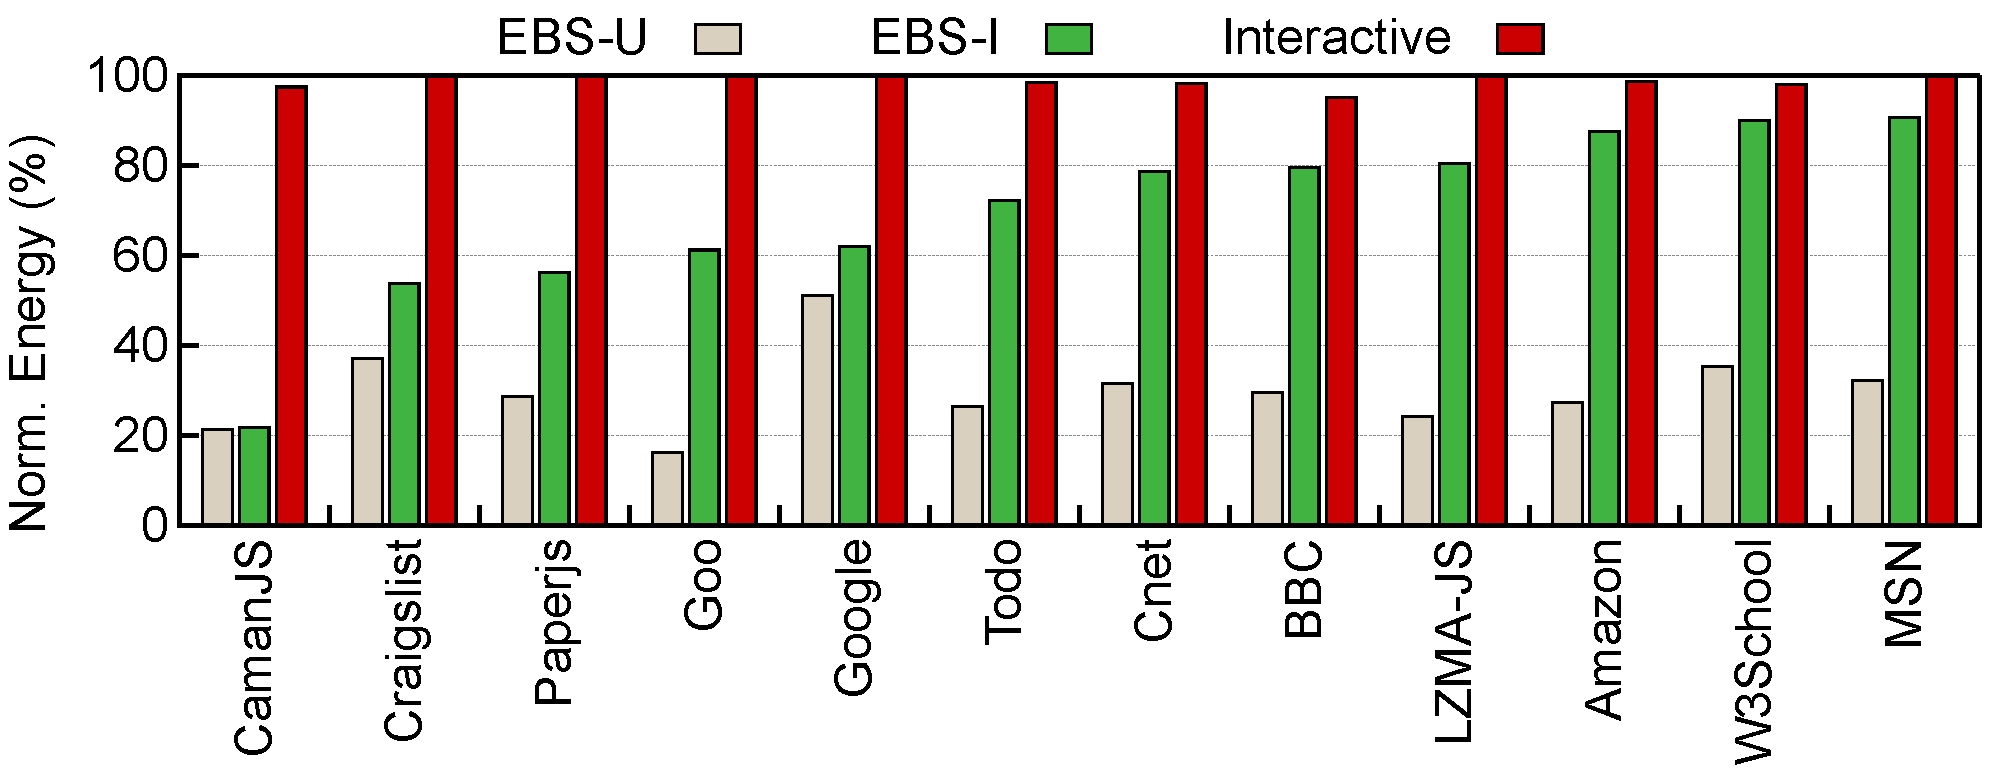
\includegraphics[trim=0 0 0 0, clip, width=\columnwidth]{energy_results_f}
\caption{Energy consumption normalized to \textit{Perf}. Lower is better.}
\label{fig:energy_results_f}
\end{figure}

\subsection{Evaluation}
\label{sec:runtime:ebs:eval}

\begin{figure}[p]
\centering
\subfloat[Architecture configuration distribution for \textit{\ebs-I}.]
{
        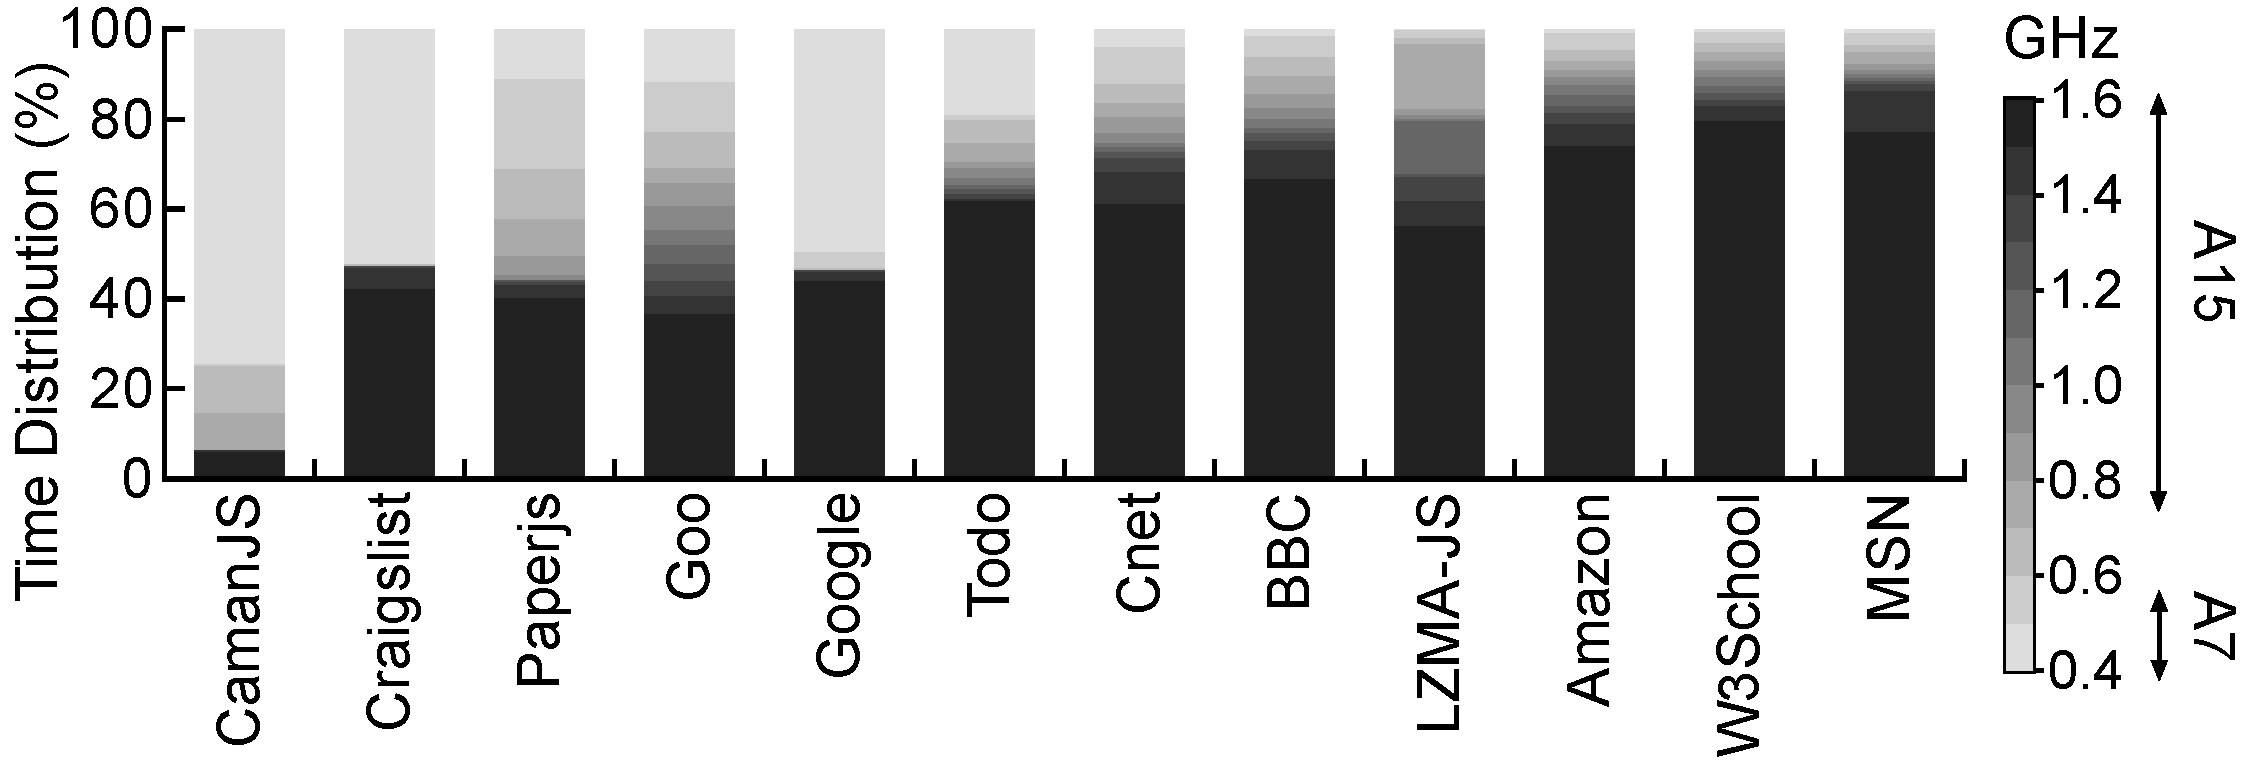
\includegraphics[trim=0 0 0 0, clip, width=\columnwidth]{freq_dist_pi}
        \label{fig:freq_dist_pi}
}\\
\vspace*{25pt}
\subfloat[Architecture configuration distribution for \textit{\ebs-U}.]
{
        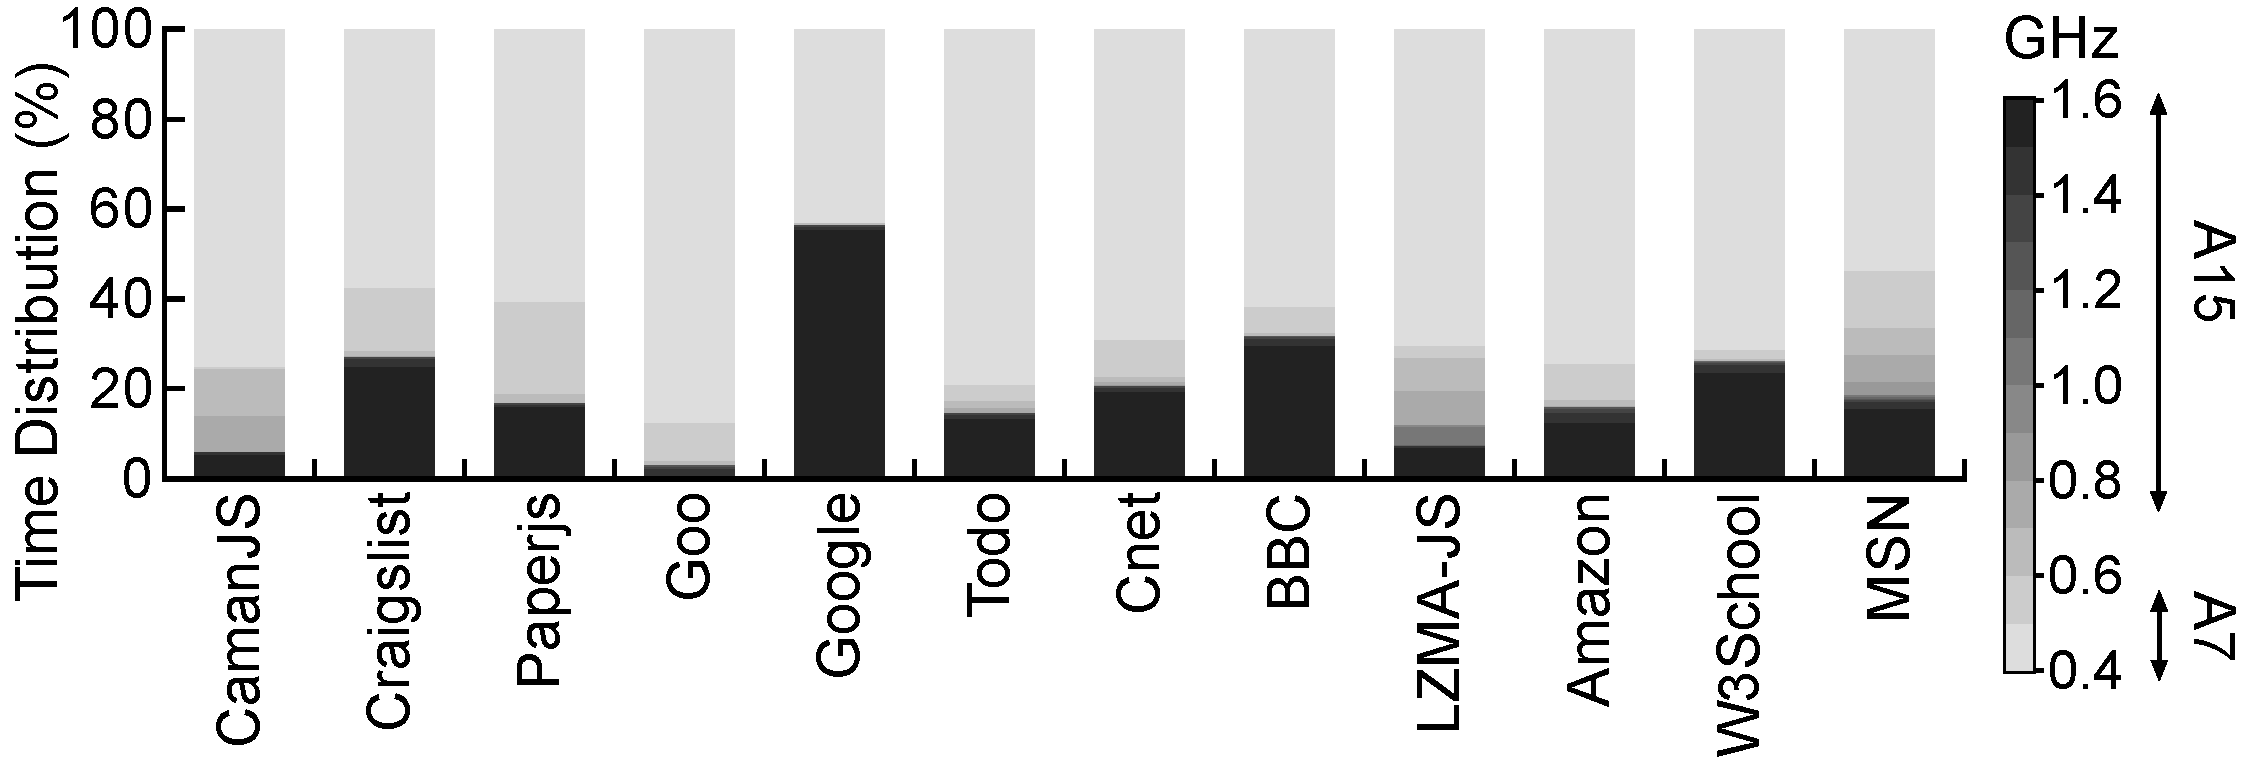
\includegraphics[trim=0 0 0 0, clip, width=\columnwidth]{freq_dist_pu}
        \label{fig:freq_dist_pu}
}
\caption{The architecture configuration distribution under the ``imperceptible'' (\textit{\ebs-I}) and ``usable''  (\textit{\ebs-U}) usage scenario.}
\label{fig:freq_dist}
\end{figure}

In this section, we perform a sequence of interactions on each application, and evaluate the end-to-end behavior of \ebs. Each sequence consists of a mix of LTM interactions and contains events with different QoS types and QoS targets. The ``Full Interaction'' category in \Tbl{tab:app} shows the details of each interaction. On average, each interaction sequence triggers about 94 events and lasts about 43~s.

We acknowledge that there are alternative ways to interact with each application. Thoroughly evaluating all the representative interactions with each application involves a large user study and is beyond the scope of this paper. However, we did perform our due diligence to make sure that the chosen interaction for each application is representative.

\paragraph{Energy Savings} \Fig{fig:energy_results_f} shows the energy consumption of \textit{Interactive} and \ebs's two usage scenarios. The results are normalized to \textit{Perf}, and sorted in the ascending order of \textit{\ebs-I}. As compared to \textit{Interactive}, \ebs achieves on average 29.2\% and 66.0\% energy saving under the imperceptible and usable usage scenarios, respectively.

\textit{Interactive} consumes energy close to \textit{Perf} across all applications, indicating that the Android \texttt{Interactive} governor is almost always operating at the peak performance. This is because user interactions, especially events with a ``continuous'' QoS type, typically generate a large volume of frames, which leads to high CPU utilization. \textit{Interactive} responds to the high CPU utilization by increasing CPU performance. With the QoS knowledge provided by developers, however, \ebs can identify execution configurations that conserve energy while still meeting QoS requirements.

\paragraph{Architecture Configuration Distribution} To better understand the sources of energy savings of \ebs , we examine the architecture configuration distribution of \ebs under the imperceptible and usable usage scenario shown in \Fig{fig:freq_dist_pi} and \Fig{fig:freq_dist_pu}, respectively. Bars with darker colors indicate higher performance configurations.

We make two notable observations from the distribution results. First, \ebs tends to bias toward big core (A15) configurations much more often under the imperceptible scenario (\Fig{fig:freq_dist_pi}) than under the usable scenario (\Fig{fig:freq_dist_pu}). This observation confirms the result that \textit{\ebs-I} has less energy saving than \textit{\ebs-U}. Second, the fact the \ebs dynamically changes its execution configuration under different QoS targets indicates that the \ebs can adapt to different user QoS expectations while saving energy. In contrast, \textit{Interactive} always adopts the same scheduling policy independent of the user QoS expectation, leading to energy waste. This observation indicates that an ACMP architecture is beneficial in mobile Web, but the burden is on the runtime system to intelligently leverage it.

\begin{figure}[t]
  \centering
  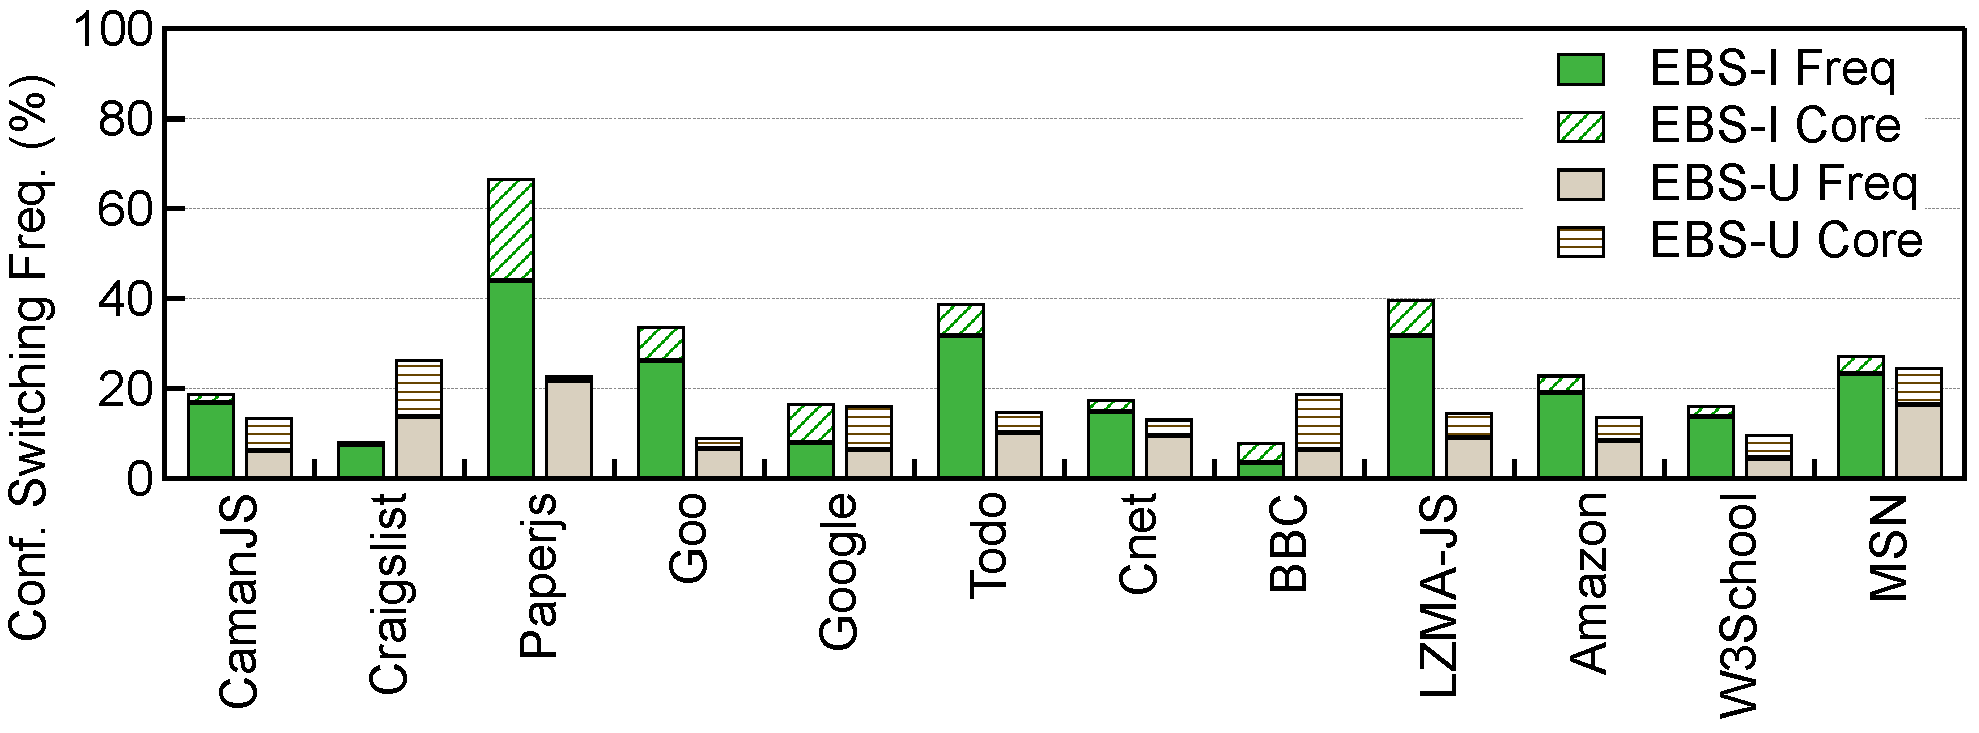
\includegraphics[trim=0 0 0 0, clip, width=\columnwidth]{freq_switch}
  \caption{Execution configuration switching frequency under \textit{\ebs-I} and \textit{\ebs-U}. Two configuration switching types exist: CPU frequency switch (solid) and core migrations (stripe).}
  \label{fig:freq_switch}
\end{figure}

\paragraph{Configuration Switching Frequency} Complementary to the distribution of architecture configuration, \Fig{fig:freq_switch} shows the switching frequency of architecture configuration in \textit{\ebs-I} and \textit{\ebs-U}. We decompose the configuration switching into two categories: CPU frequency change and core migration (between big and little clusters). Thus, \Fig{fig:freq_switch} is shown as a stacked bar plot where the frequencies of both categories are stacked for each application.

\begin{figure}[p]
\centering
\subfloat[QoS violation comparison under the imperceptible usage scenario.]
{
        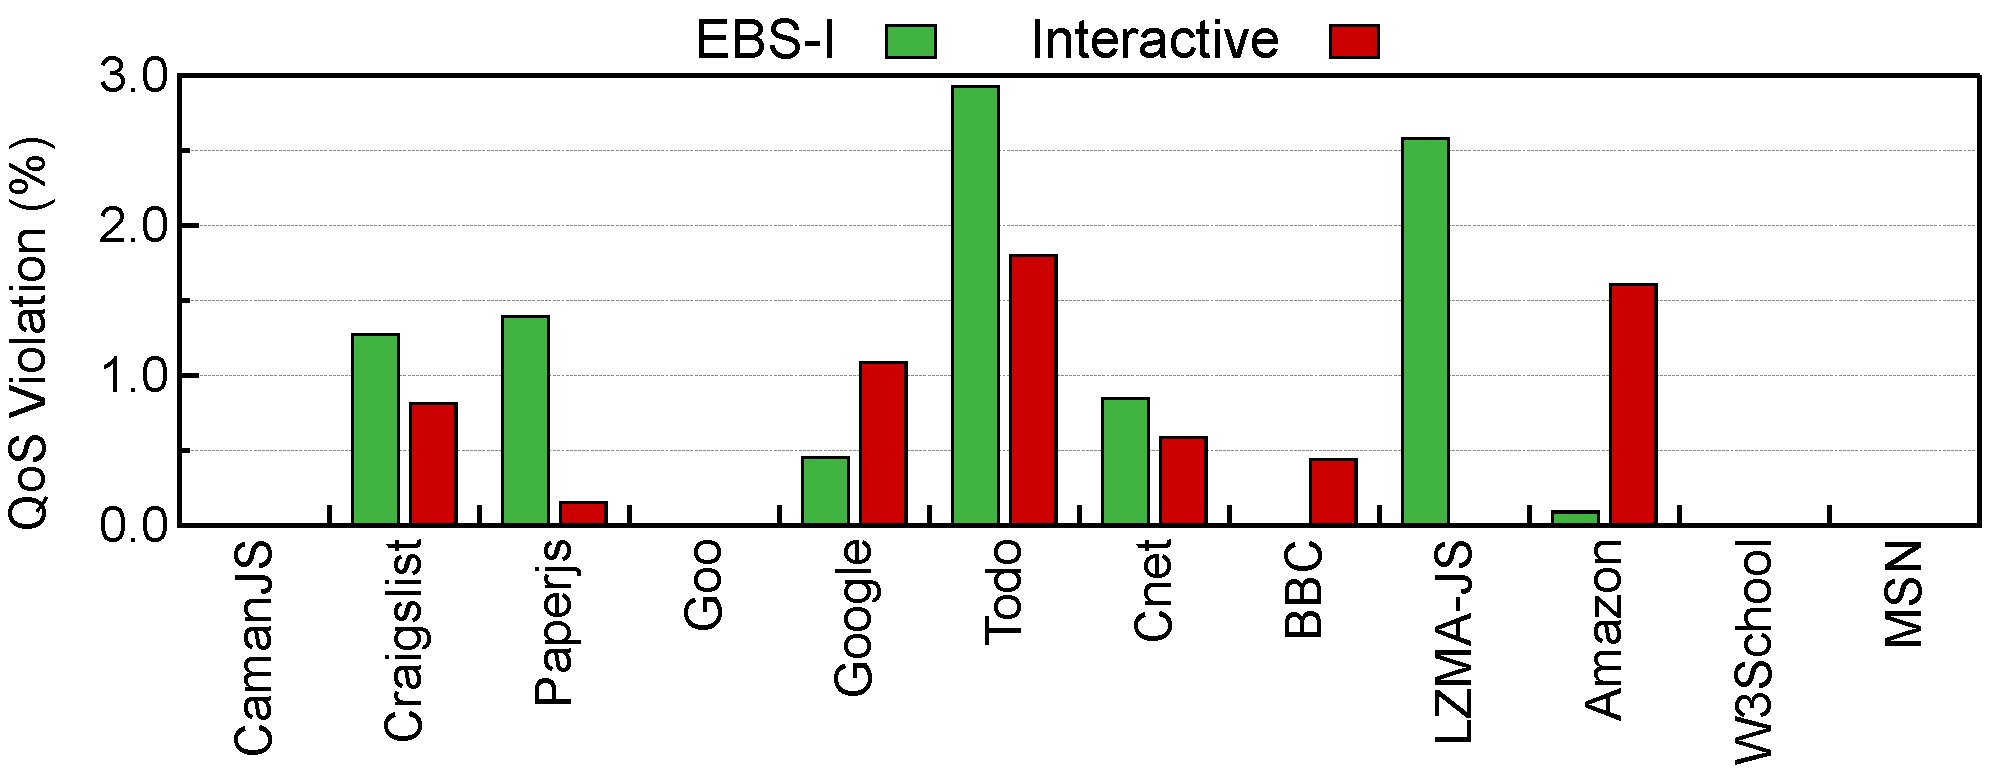
\includegraphics[trim=0 0 0 0, clip, width=\columnwidth]{qos_pi_results_f}
        \label{fig:qos_pi_results_f}
}\\
\vspace*{25pt}
\subfloat[QoS violation comparison under the usable usage scenario.]
{
        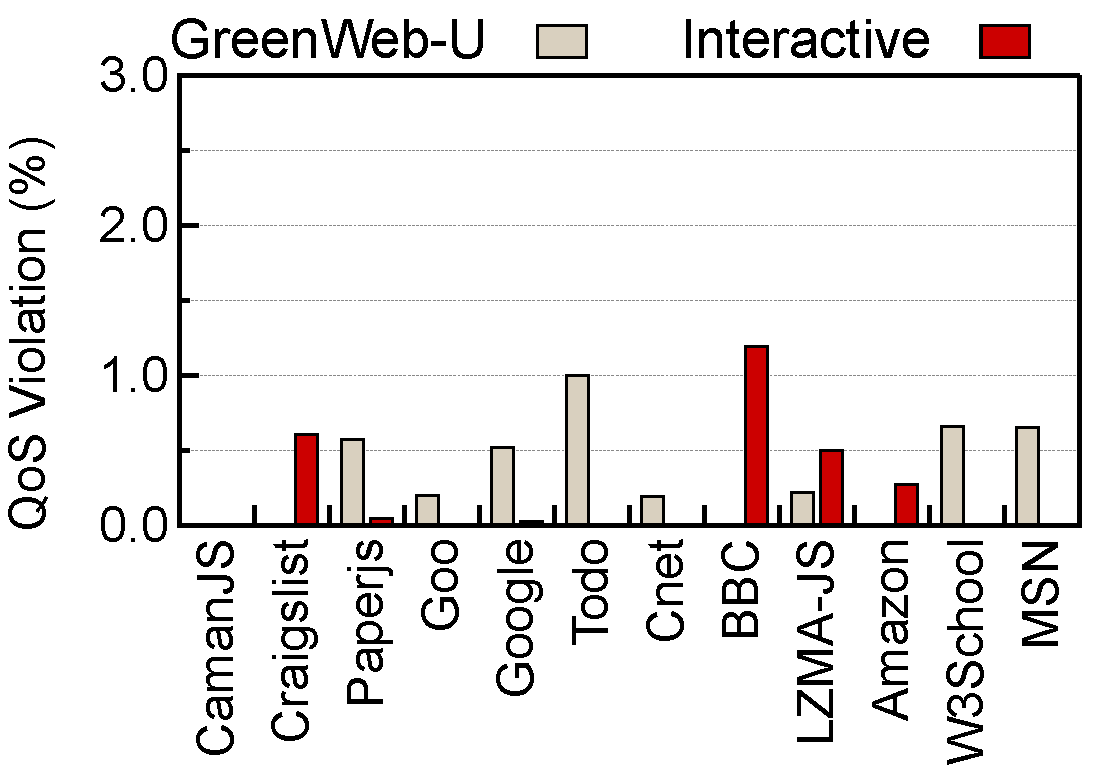
\includegraphics[trim=0 0 0 0, clip, width=\columnwidth]{qos_pu_results_f}
        \label{fig:qos_pu_results_f}
}
\caption{QoS violations are presented as additional violations on top of \textit{Perf}. The $y$-axis of the two figures are kept the same for comparion purposes.}
\label{fig:full_results}
\end{figure}

We draw three conclusions from the switching frequency statistics. First, \ebs introduces only modest configuration switching (20\% on average). Recall from \Sect{sec:runtime:exp} that the CPU frequency switching and core migration incur overhead only to the order of $\mu$s, much smaller than the QoS target which is typically to the order of millisecond. Therefore, the execution configuration has minimal performance impact.

Second, for most of applications \textit{\ebs-I} incurs more switchings than \textit{\ebs-U}. This is unsurprising because as compared to \textit{\ebs-U}, \textit{\ebs-I} optimizes for a tighter QoS target, which is more sensitive to frame (phase) variance and more vulnerable to frame performance mis-prediction. In contrast, a more relaxed QoS target is more robust against frame variance. Our results suggest that a better frame performance predictor such as the profiling-guided prediction~\cite{pgdvfs} would be helpful in reducing the execution configuration switching in the imperceptible mode.

Third, the CPU frequency change dwarfs core migrations and dominates the configuration switching. Thus, fast DVFS is desired. Our results suggest that a fast on-chip voltage regulator that is increasingly prevalent in server processors~\cite{fivr,ivr} is also beneficial in mobile CPUs.

\paragraph{QoS Violation} \Fig{fig:qos_pi_results_f} and \Fig{fig:qos_pu_results_f} show the QoS violation of \textit{Interactive} and \ebs under the imperceptible and usable scenarios, respectively. On average, \ebs introduces 0.8\% and 0.6\% more QoS violations than \textit{Perf} under the imperceptible and usable scenarios, respectively. The QoS violations are lower than in the microbenchmarks because the interaction duration gets longer and the QoS violations caused by profiling runs are amortized.

Compared to \textit{Interactive}, \ebs has similar, in some cases fewer, QoS violations. Considering the significant energy savings, we conclude that the QoS-aware \ebs system can use energy more wisely by being aware of user QoS expectations. Overall, \ebs achieves better energy efficiency than the QoS-agnostic \textit{Interactive} scheme.

\section{Related Work}
\label{sec:runtime:related}

We first discuss prior scheduling work on ACMP because the particular implementation of \webrt presented in this work relies on the ACMP architecture (\Sect{sec:runtime:related:sched}). As the goal of \webrt is to save energy without sacrificing performance, we then discuss prior work on improving the performance (\Sect{sec:runtime:related:perf}) and energy consumption (\Sect{sec:runtime:related:energy}).

\subsection{Single ISA/DVFS Scheduling}
\label{sec:runtime:related:sched}

The particular implementation of \webrt is an example of utilizing single-ISA heterogeneous systems capable of DVFS for trading off performance with energy~\cite{single-ISA}. Nvidia's Kal-El~\cite{Tegra3} is a single-ISA heterogeneous system that integrates four high-frequency cores with one low-frequency core. ARM's proposed big.LITTLE system~\cite{big.little} contains an out-of-order Cortex-A15 processor and an in-order Cortex-A7 processor. ACMP architecture is already widely adopted in today's mobile SoCs shipped by major vendors such as Samsung and Qualcomm~\cite{exynos5biglittle}. We expect our \webrt implementation to be readily applicable to commodity mobile hardware.

The scheduling mechanism in \webrt differs from existing single-ISA scheduling and DVFS techniques in three key aspects: scheduling \textit{unit}, scheduling \textit{objective}, and scheduling \textit{heuristics}. First, the scheduling unit in existing techniques is either interval based (fixed-instruction interval~\cite{single-ISA,compositecores,tracephase,tm,DVFSPred} or fixed-time interval~\cite{DCS,MIPJ,PIE,ondemand,unfairsched}) or a code segment (e.g., critical sections, lagging threads, application kernels~\cite{acs,bis,uba,YinYang}). The scheduling unit in the \webrt is Web application-specific entities: event handlers in event-based scheduling and webpage loadings in webpage-aware scheduling. These Web application-specific units directly correspond to user interactions and let us directly optimize for user QoS experience.

Second, the scheduling objectives in existing techniques are typically architecture-level energy-efficiency metrics such as energy, EDP~\cite{edp}, and million-instructions-per-joule (MIPJ)~\cite{MIPJ}. These metrics trade off raw performance instead of QoS with energy. Therefore, they may lead to executions that fall into the imperceptible or unusable QoS regions and waste energy. On the contrary, \webrt scheduler  aims at minimizing energy consumption under explicit performance constraint in order to guarantee satisfactory QoS experience.
%In addition, we also propose a metric called QPE, which could be directly used as a scheduling objective for trading off QoS with energy consumption.

Third, the webpage-aware scheduler's prediction-based scheduling heuristics is similar to other recent heterogeneous scheduling proposals in the architecture community \cite{PIE,compositecores,tracephase,tm}. In contrast, instead of relying on (micro)architecture- and system-level statistics for prediction, the webpage-aware scheduler captures the complex behavior of webpage characteristics using regression modeling, and accurately predicts the webpage load time and energy consumption.

Timer coalescing~\cite{powerinosx} used in OS X Mavericks also exploits the performance slack for energy savings, similar to our event-based scheduling. It postpones noncritical timers and coalesces them for batch executions to increase the processor idle time for energy savings. However, timer coalescing applies only to timers in Apple's native applications (or OS processes), whereas our EBS framework is not limited to timer events, but can apply to any event-driven applications.

\subsection{Web Performance Optimizations}
\label{sec:runtime:related:perf}

Most prior research focus on parallelizing browser tasks, such as parsing, CSS selection, etc.~\cite{ParallelBrowser,FTL,UCI,Parabix}. Although such parallelized algorithms can achieve speedups ranging from 4X to 80X for various browsing tasks, they typically do not scale well beyond four cores with the expense of potential energy inefficiency. Thus, while parallelization has potential in desktop systems, it is less favorable for mobile Web computing.

Another portion of performance optimizations focuses on improving the execution model of the Web browser through asynchronous/multiprocess rendering, resource prefetching, smarter browser caching, etc.~\cite{pocketweb,Adrenaline,smart-caching,webkit2,firefox-spec_parsing}. All these techniques are orthogonal and can be integrated with my proposal, which primarily focused on the core rendering engine of a Web browser.

\subsection{Web Energy Optimizations}
\label{sec:runtime:related:energy}

Thiagarajan~et al.~\cite{www-battery} break the Web browser's energy consumption into coarser-grained elements, such as CSS and Javascript behavior, and identify a few system- and application-level optimizations to improve the energy consumption of mobile Web browsing.  The optimizations they recommend, such as reorganizing JavaScript files and removing unnecessary CSS rules, are orthogonal and complementary to our webpage prediction and scheduling work. Other works analyze the power/energy consumption of the entire smartphone\cite{Carroll,eprof,JamesHotchip}, whereas we focus on improving the energy-efficiency of the mobile processor in response to the demand for high-performance.

Another body of energy-related research focuses on diagnosing energy bugs and hogs in mobile applications. These techniques either completely kill an energy-hungry application~\cite{carat} or require developers to improve manually the energy efficiency~\cite{energygreedapis,eprof,eLens}. \webrt eases developers' effort by automatically optimizing for energy efficiency.


%!TEX root=../paper.tex

\chapter{GreenWeb: Web Language Extensions for Energy-Efficient Web Computing}
\label{sec:lang}

%Web application developers today must be conscious of energy efficiency. Current abstractions between software and hardware, however, do not provide developers opportunities to optimize for energy efficiency. Instead, energy optimizations are mostly conducted at the hardware and OS level via techniques such as dynamic voltage and frequency scaling. Although effective from a hardware perspective, the key limitation of these techniques is that they are not aware of user quality-of-service (QoS) expectation and may lead to poor experience~\cite{big-little, ebs, pgdvfs}. Failing to deliver desirable QoS experience can cause severe consequences. For example, a 1-second delay in webpage load time costs Amazon \$1.6 billion annual lost in sales~\cite{Eaton:2013uq}.

Web languages are at the interface between applications and Web runtime. Traditionally, Web developers use Web languages to express structure, style, and functionality of an application while relying on the underlying system to perform energy optimizations without compromising user QoS experience. However, as mobile users become increasingly aware of poor energy behavior of applications~\cite{badappreviews,appdeletion}, Web developers today must be  explicitly conscious of energy efficiency. Current programming language abstractions, however, provide developers few opportunities to optimize for energy efficiency. Instead, energy optimizations are mostly conducted at the hardware and OS level via techniques such as dynamic voltage and frequency scaling. Although effective from a system perspective, the key limitation of these techniques is that they are not aware of user quality-of-service (QoS) expectations and may lead to poor experience~\cite{big-little,ebs,pgdvfs}. Failing to deliver a desirable QoS experience can cause severe consequences. For example, a 1-second delay in webpage load time costs Amazon \$1.6 billion annual sales lost~\cite{Eaton:2013uq}.

In this chapter, I present \greenweb, a set of Web language extensions defined as Cascading Style Sheet (CSS) rules that allow Web developers to express user QoS expectation at an abstract level. Based on the programmer-guided QoS information, the runtime substrate of \greenweb could then dynamically determine how to deliver the target QoS experience while minimizing the energy consumption.

To help Web developers reason about QoS constraints in Web applications, our \textit{key insight} is that user QoS experience can be sufficiently captured by two fundamental abstractions: \textit{QoS type} and \textit{QoS target}. Intuitively, QoS type characterizes whether users perceive QoS experience by interaction responsiveness or animation smoothness, and QoS target denotes the performance level that is required to deliver a desirable user experience for a specific QoS type. \greenweb provides specific language constructs for expressing the two QoS abstractions and thus empowering Web developers to provide ``hints'' to guide energy optimizations.

Allowing programmers to annotate QoS information in applications is both \textit{precise} and \textit{efficient}. It is precise because only developers have the exact knowledge of code logic. They can provide QoS type and target information that is difficult for the runtime to infer. It is efficient because it does not entail performance and energy overhead of runtime detection. Such a design philosophy is similar to traditional pragma-based programming APIs such as OpenMP. For example, the ``\texttt{omp for}'' pragma in OpenMP indicates that iterations in a \texttt{for} loop are completely independent such that the runtime can safely parallelize the loop without the need to check for correctness. Similarly, \greenweb annotations would allow the Web runtime to perform ``best-effort'' optimizations without having to infer QoS information.

The rest of this chapter is organized as follows. \Sect{sec:lang:eqos} discusses the relationship between QoS, performance, and energy consumption. It lays the foundation of abstracting user QoS experience. \Sect{sec:lang:abst} defines two abstractions that are critical to mobile user QoS experience, and \Sect{sec:lang:spec} describes the proposed \greenweb language constructs that express the two abstractions. \Sect{sec:lang:auto} presents \autogreen to demonstrate the feasibility of automatically applying \greenweb annotations to a Web application. \Sect{sec:lang:inter} discusses the relationship between the \greenweb extensions and the \webrt runtime, and argue that \greenweb and \webrt are synergistic while independent. \Sect{sec:lang:disc} discusses the implications and limitations of the current design and implementation of \greenweb. Finally, \Sect{sec:lang:related} puts \greenweb in the general context of language support for performance and energy-efficiency.

\section{Trade-off Between QoS, Performance, and Energy}
\label{sec:lang:eqos}

We illustrate the relationship between application QoS, performance, and energy savings in~\Fig{fig:eqos}. Performance degrades from left to right on the~\textit{x}-axis. The left and right~\textit{y}-axes indicate QoS and energy savings, respectively. Foundational work in human-computer interaction research~\cite{eventlatency,designUI,info_vis,response_time,percent_done,usability_engineering} indicates that interactive application QoS can be classified into three distinct states as machine performance degrades: \textit{imperceptible} $[P_H,P_I]$, \textit{tolerable} $(P_I,P_U]$, and \textit{unusable} $(P_U,P_L]$.

\begin{figure}[t]
\centering
\captionsetup{width=.9\columnwidth}
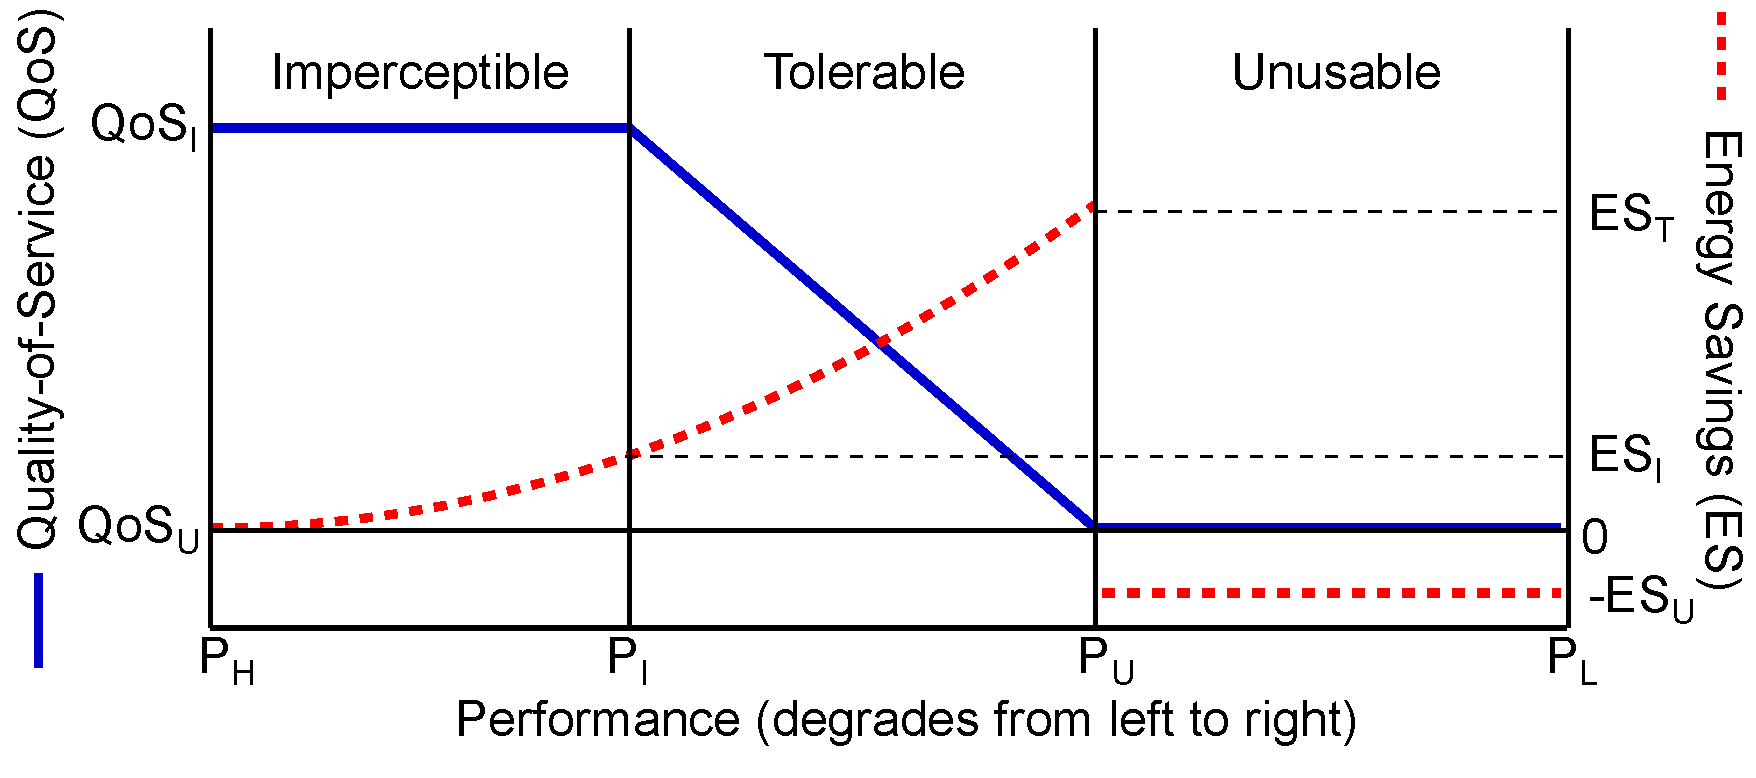
\includegraphics[trim=0 0 0 0, clip, width=.9\columnwidth]{eqos}
\caption{The interplay between QoS, performance, and energy.}
\label{fig:eqos}
\end{figure}

In the imperceptible region, performance can degrade without any user-perceptible QoS loss while achieving more energy savings. Imperceptible QoS, $QoS_I$, is maintained until performance reaches $P_I$, the lowest performance level that provides $QoS_I$. In the imperceptible region, supplying higher performance simply leads to more energy waste without adding any end-user value. For example, the most conservative approach to guarantee application QoS is to supply the peak performance of $P_H$; it leads to an energy waste of $ES_I$. Beyond $P_I$, application QoS enters the tolerable region, where QoS deteriorates as performance reduces, but still remains tolerable. Any QoS could be acceptable in this region depending on the usage scenario or specific user pattern~\cite{usagepattern,satscore}. Therefore, the tolerable QoS region exhibits a traditional performance-energy trade-off space. As performance further degrades, QoS is eventually violated at $P_U$, which is the performance limit where users no longer feel engaged by the application. At $P_U$ and beyond, users abandon the service. As a result, any energy consumed up until the service abandonment ($ES_U$) is wasted, because the underlying computation does not provide any utility to the user.

In summary, QoS-aware energy-efficiency optimization implies one of the following two optimization strategies depending on user QoS expectation. First, when the QoS expectation is high, guarantee imperceptible QoS experience with the minimal energy by exploiting the performance slack between $P_H$ and $P_I$. Second, when the user QoS expectation is low, guarantee usable QoS experience with the minimal energy by achieving a performance of $P_U$.

\section{QoS Abstractions for Web Applications}
\label{sec:lang:abst}

Expressing user QoS experience to the underlying system is the key in QoS-aware energy efficiency optimizations. However, today's Web languages do not allow expressing QoS information. Programmers need new \textit{abstractions}. We propose two abstractions, QoS type and QoS target, that capture two fundamental aspects of user QoS experience in Web applications. Such QoS abstractions hide the complexity of the specific application implementation from underlying systems while still providing enough details to guide energy optimizations. This section introduces the abstractions, and the next section~(\Sect{sec:lang:spec}) describes the proposed language constructs that enable programmers to express the abstractions.

Abstracting user QoS experience requires us to first understand how users assess QoS experience in mobile Web applications. To that end, we leverage the LTM user-application interaction model described in \Sect{sec:runtime:overview}. The LTM model captures three fundamental user interactions in mobile Web applications (Loading-Tapping-Moving) and gives us a framework for reasoning about user QoS experience. Based on the LTM model, we propose the QoS type~(\Sect{sec:lang:abst:type}) and QoS target~(\Sect{sec:lang:abst:target}) abstractions. We discuss why they are necessary and sufficient to express QoS information for QoS-aware energy efficiency optimizations.

\subsection{QoS Type}
\label{sec:lang:abst:type}

We define an abstraction called \textit{QoS type} to capture different ways that users interpret the QoS experience. Two major QoS types exist: \textit{single} and \textit{continuous}. Intuitively, they indicate whether the QoS experience is determined by the ``responsiveness'' of a single frame or the ``smoothness'' of a continuous sequence of frames, respectively. Let us use the LTM model to elaborate on the two QoS types.

%!TEX root=../../paper.tex

\begin{table}[t]
\large
\centering
\caption{Interactions in mobile Web applications fall into three categories based on different QoS type and QoS target combinations.}
\renewcommand*{\arraystretch}{1.2}
\renewcommand*{\tabcolsep}{10pt}
\resizebox{\columnwidth}{!}
{
  \begin{tabular}{l l l c}
  \toprule[0.15em]
  \bigstrut\textbf{QoS Type} & \bigstrut\textbf{\specialcell{QoS Target\\($P_I$, $P_U$)}} & \multicolumn{1}{c}{\bigstrut\textbf{~~~~~~~~Description}} & \bigstrut\textbf{Interaction}\\
  \midrule[0.05em]
  Continuous & (16.6, 33.3) ms & \specialcell{QoS experience is evaluated\\by \textit{continuous} frame latencies.} & T, M\\
  \midrule
  \multirow{2}{*}[-23pt]{Single} & (100, 300) ms & \specialcell{QoS experience is evaluated
\\by \textit{single} frame latency. Users
\\expect \textit{short} response period.} & T \\ \cline{2-4}
  & (1, 10) s & \specialcell{QoS experience is evaluated
\\by \textit{single} frame latency. Users
\\expect \textit{long} response period.} & L, T \\
  \bottomrule[0.15em]
  \end{tabular}
}
\label{tab:qos_info}
\end{table}



\paragraph{Single} Some user interactions produce only a single frame, which we call the response frame. The QoS type of these interactions is ``single,'' indicating that user QoS experience is determined by the latency at which the response frame is perceived by users~\cite{eventlatency}. For instance, imagine a fingertap interaction (T) that opens a search box in a Web application. Users perceive the effect of the fingertap when the application displays a response frame---the frame with the search box displayed. Web application loading process (L) also falls in this category. This is because although there are several intermediate frames being produced during the loading process, user QoS experience is largely determined by the latency of the ``first meaningful frame''~\cite{fmf}, which indicates that a Web application is usable by users.

Under the ``single'' QoS type, an ideal energy-efficient system would allocate just enough energy to produce the single response frame and conserve energy afterwards. It is worth noting that the system might not be completely idle after the response frame is delivered. The system could still perform work such as updating the browser cache, performing garbage collection, or rasterizing off-screen pixels. Such ``post-frame'' work is not critical to user QoS experience and could be executed in a low-power mode.

\paragraph{Continuous} The other QoS type is ``continuous,'' corresponding to interactions whose responses are not one single frame but a sequence of continuous frames. User QoS experience is determined by the latency of \textit{each} frame in the sequence rather than one specific frame as in the ``single'' case. Ideally, an energy-efficient Web runtime would allocate just enough energy for each frame in the sequence and conserve energy after all the frames are produced.
%Determining the exact sequence of frames given an input event is a non-trivial task and we discuss it in \Sect{sec:runtime:frame}.

Continuous frames are often found in the form of animations. The simplest form of animation is triggered by finger moving (M) such as scrolling. Tapping (T) can also cause a sequence of frames to be generated. For instance, many Web applications provide a navigation button that dynamically expands when tapped and generates an animation. More complex animations in Web applications can be controlled by \texttt{requestAnimationFrame} (\texttt{rAF}) APIs~\cite{animationtiming} and CSS animation/transition~\cite{cssanimations,csstransitions}.

Distinguishing between ``continuous'' and ``single'' is important. If an event callback triggers an animation but the runtime treats its QoS type as ``single'', the runtime would optimize for only the first frame in the sequence, and thus mis-operates for the remaining frames. On the other hand, if an event produces only a single frame followed by some ``post-frame'' work, a runtime (mistakenly) optimizing for ``continuous'' frame latency would force the hardware to run at the peak performance to execute the ``post-frame'' work (with the intention of generating more frames), leading to energy waste. Whether an event triggers a single frame or a sequence of frames can not be determined a priori. In \Sect{sec:lang} we will introduce a set of language extensions that let developers explicit specify an event's QoS type, through which the runtime could be better informed in optimizations.

\subsection{QoS Target}
\label{sec:lang:abst:target}

Another critical QoS abstraction is \textit{QoS target}, denoting the performance level needed to deliver a certain QoS experience. We use frame latency as a natural choice for the performance metric because frame updates dictate QoS experience. Specifically, we define frame latency as the delay from when an event is initiated by a user to when its corresponding frame(s) show on the display.

Two different QoS targets exist that are critical to user experience: imperceptible target ($P_I$) and usable target ($P_U$)~\cite{ebs}. Imperceptible target delivers a latency that is imperceptible/instantaneous to users. Achieving a performance higher than $P_I$ does not add user perceptible value while unnecessarily wasting energy. The usable target, in contrast, corresponds to a latency that can barely keep users engaged. Delivering a performance lower than $P_U$ may cause users to deem an application unusable and even abandon it.

\paragraph{Single} For interactions with the ``single'' QoS type, QoS target depends on the complexity of the interaction~\cite{eventlatency}. For interactions that are expected to finish quickly, user latency tolerance is low. For instance, a fingertap that displays a search box falls into this category, because displaying a search box is inherently expected to finish ``instantly.'' For these ``lightweight'' interactions, users feel the system is responding instantly at 100~ms, and start thinking that the system is not working after 300~ms~\cite{humanperception}. Thus, 100~ms and 300~ms can be used as the $P_I$ and $P_U$ values, respectively.

In contrast, when users are aware of a computationally intensive job being processed, they tend to have high tolerance for latencies~\cite{usability_engineering}. Psychological study shows that users can subconsciously wait up to 1 second for a job to complete while still staying focused on the current train of thought. Once a job execution exceeds 10 seconds, user attentions are distracted and cannot tolerate the delay~\cite{info_vis,response_time}. Therefore, 1 second and 10 seconds can be treated as the $P_I$ and $P_U$ values for ``heavyweight'' interactions, respectively.

\paragraph{Continuous} For interactions with a ``continuous'' QoS type, 60 and 30 frames per second (FPS) deliver a ``seamless'' and ``just playable'' user experience, respectively~\cite{fps_target}. Thus, a performance level that guarantees 16.6~ms and 33.3~ms frame latency can be regarded as the imperceptible and usable QoS target, respectively. It is worth noting that the QoS target applies to each frame rather than an average latency. This is because human eyes are very sensitive to frame variance. Tiny hitches in a high volume of frames can cause a poor QoS experience and even headaches~\cite{jankbusting,adaptivevsync}.

User interactions fall into three distinct categories based on the different QoS type and QoS target combinations as listed in \Tbl{tab:qos_info}. Although the absolute values of QoS target ($P_I$ and $P_U$) in each category can vary slightly with user perceptibility, their magnitudes differ significantly across categories (i.e., tens of milliseconds versus hundreds of milliseconds versus seconds). Thus, QoS target is an important abstraction to differentiate different performance requirements.

\section{QoS-Aware Web API Design}
\label{sec:lang:spec}

We now present \greenweb, a set of Web language extensions that lets application developers easily express the two QoS abstractions as program annotations. We first discuss the design principles of \greenweb extensions (\Sect{sec:lang:spec:principles}). We then describe the design and specification of \greenweb~(\Sect{sec:lang:spec:api}). We then present usage scenarios to demonstrate the expressiveness and modularity of the \greenweb design~(\Sect{sec:lang:spec:ex}).

\subsection{Design Principles}
\label{sec:lang:spec:principles}

\greenweb extensions follow three design principles. First, adding or removing \greenweb annotations does not change application functionality and correctness. In other words, \greenweb annotations are \textit{modular} components in an application. Modularity allows developers who are unfamiliar with application logic to still be able to express QoS information, and allows removing problematic annotations in a non-interference manner.

Second, \greenweb is \textit{intuitive} for Web application developers to use in that it does not require developers to specify absolute values of QoS targets (although this option is provided if needed). This is important because developers may not have quantitative knowledge about user perceptibility. Instead, developers provide a qualitative specification. This design makes the APIs more expressive, and provides flexibility for runtime implementation. 

Third, \greenweb syntax is \textit{compatible} with current Web language specifications, which is crucial for lowering the learning curve and ensuring programmer productivity.

\subsection{QoS-Aware Web API Design}
\label{sec:lang:spec:api}

% !TEX root = ../../paper.tex

\begin{table}[p]
\large
\centering
\caption{Specifications of the \greenweb APIs. Each API is a new CSS rule specifying the QoS information when a particular event is triggered on certain Web application element.}
\renewcommand*{\arraystretch}{1.1}
\renewcommand*{\tabcolsep}{8pt}
\resizebox{\columnwidth}{!}
{
    \begin{tabular}{l l}
    \toprule[0.15em]
    \bigstrut\textbf{Syntax} & \bigstrut\textbf{Semantics} \\
    \midrule[0.05em]
    \specialcell{\texttt{\textcolor{blue}{E:QoS} \{}
\\~~~~\texttt{\textcolor{Green}{onevent-qos:} continuous}
\\\texttt{\}}} & \specialcell{As soon as \texttt{onevent} is triggered on\\DOM element \texttt{E}, the application must\\continuously optimize for frame latency.\\Use the $P_I$ and $P_U$ values in \Tbl{tab:qos_info} as\\the default QoS target for all frames.}\\
    \midrule[0.05em]
    \specialcell{\texttt{\textcolor{blue}{E:QoS} \{}
\\~~~~\texttt{\textcolor{Green}{onevent-qos:} single,}
\\~~~~\texttt{~~~~~~~~~~~~~~short|}
\\~~~~\texttt{~~~~~~~~~~~~~~~long}
\\\texttt{\}}} & \specialcell{Once \texttt{onevent} is triggered on element\\\texttt{E}, the application must optimize for the\\latency of the single frame caused by\\ \texttt{onevent}. Users expext short (long)\\latency. Use the $P_I$ and $P_U$ values in\\\Tbl{tab:qos_info} as the default QoS target.}\\
    \midrule[0.05em]
    \specialcell{\texttt{\textcolor{blue}{E:QoS} \{}
\\~~~~\texttt{\textcolor{Green}{onevent-qos:} continuous|}
\\~~~~\texttt{~~~~~~~~~~~~~~~~~single,}
\\~~~~\texttt{~~~~~~~~~~~~~~~ti-value,}
\\~~~~\texttt{~~~~~~~~~~~~~~~tu-value}

\\\texttt{\}}} & \specialcell{Explicitly specify $P_I$ (\texttt{ti-value}) and\\$P_U$ values (\texttt{tu-value}) for QoS targets.\\Note that both values must either appear\\or be ommitted together.}\\
    \bottomrule[0.15em]
    \end{tabular}
}
\label{tab:api_spec}
\end{table}


\begin{figure}[t]
  \centering
  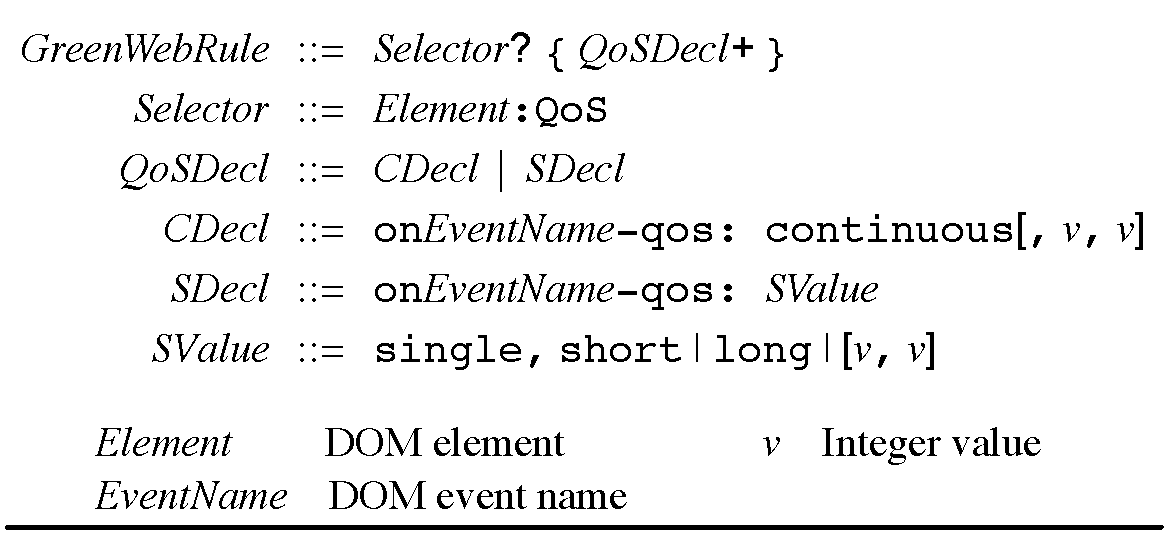
\includegraphics[trim=0 0 0 0, clip, width=.8\columnwidth]{syntax}
  \caption{The syntax of \greenweb language extensions.}
  \label{fig:syntax}
\end{figure}

The \greenweb APIs extend the current CSS language to specify QoS type and QoS target information. We choose CSS because its syntax and semantics naturally allow us to select DOM elements and specify various characteristics. The core of CSS is a set of \textit{style rules}. Each style rule selects specific Web application elements and sets their style properties. A style rule expresses such semantics through two language constructs: a \textit{selector}, which selects specific Web application elements, and a set of style \textit{declarations}, which are $\langle property, value \rangle$ pairs that assign $value$ to $property$. As an example, the following CSS rule \texttt{h1 \{font-weight: bold\}} selects all the \texttt{h1} elements and sets their \texttt{font-weight} property to \texttt{bold}.

Traditionally, CSS supports purely visual style properties such as fonts and colors. Recent development of CSS (e.g., CSS3) lets developers express richer information such as controlling animations~\cite{cssanimations} and adapting to different device form factors~\cite{css3mediaquery}. \greenweb follows this spirit of CSS language evolution and further expands the CSS semantics scope to allow expressing user QoS related information.

\Fig{fig:syntax} shows the \greenweb syntax, and \Tbl{tab:api_spec} lists the semantics of each API. Intuitively, each \greenweb API selects an application element \texttt{E}, and declares CSS properties to express the QoS type and QoS target information when an event \texttt{onevent} is triggered on \texttt{E}. We now describe the details of the \greenweb extensions.

\paragraph{Selector} To decorate a CSS rule as specifying the QoS information of an element, we define a new CSS pseudo-class selector~\cite{css_pseudo_class} ``\texttt{:QoS}.'' An element \texttt{E} is selected using existing selectors, such as ID (\texttt{\#id}) and Class (\texttt{.class}) selectors, before applying the \texttt{:QoS} pseudo-class qualifier. For example, \texttt{div\#intro:QoS} selects the \texttt{div} element with the ID \texttt{intro} before declaring QoS information.

\paragraph{Property} QoS information is expressed as CSS properties in \greenweb. We define a new CSS property called \texttt{onevent-qos}, in which \texttt{onevent} is a DOM event that \greenweb supports. In its simplest form, \texttt{onevent-qos} could be set to \texttt{continuous} (first rule in \Tbl{tab:api_spec}). The semantics of declaring \texttt{onevent-qos: continuous} is that as soon as \texttt{onevent} is triggered on element \texttt{E}, the Web browser runtime must continuously optimize for frame latency until the last relevant frame is generated.

To express the ``single'' QoS type, the \texttt{onevent-qos} property accepts a list of two values separated by a comma, one to indicate that the QoS type is single, and the other to indicate whether users expect a short or long execution period (second rule in \Tbl{tab:api_spec}). For instance, the declaration \texttt{onevent-qos: single, short} expresses that the runtime must optimize for the latency of the single frame caused by \texttt{onevent}, and users expect short frame latency.

Developers do not have to specify the QoS target values; the \greenweb runtime will use the $P_I$ and $P_U$ values in \Tbl{tab:qos_info} as the default QoS target. However, we also provide the flexibility for developers to overwrite the default QoS targets. This is achieved by specifying absolute values of $P_I$ and $P_U$ (in milliseconds) after \texttt{single} or \texttt{continuous}, as shown in the third rule in \Tbl{tab:api_spec}.

\subsection{Example Usage}
\label{sec:lang:spec:ex}

The proposed QoS-aware \greenweb APIs support a wide range of Web application interaction patterns. We explore different usages using two examples.

\begin{figure}[t]
\centering
\subfloat[Express the QoS type of \texttt{ontouchstart} event as ``continuous,'' and use the default $P_I$ and $P_U$ values.]
{
	\includegraphics[trim=0 0 0 0, clip, width=.45\columnwidth]{csstransition}
	\label{fig:csstransition}
}
\hspace*{15pt}
\subfloat[Express the QoS type of \texttt{ontouchmove} event as ``continuous,'' and use 20~ms and 100~ms as the new QoS targets.]
{
	\includegraphics[trim=0 0 0 0, clip, width=.45\columnwidth]{raf}
	\label{fig:raf}
} 
\caption{Example \greenweb usage.}
\label{fig:ex}
\end{figure}

\paragraph{Animations via CSS Transition} The first example involves annotating events that achieve animation using a CSS transition. A CSS transition lets developers specify the initial and end state of an animation and how long the transition takes, while leaving the transition implementation to the Web browser~\cite{csstransitions}. \Fig{fig:csstransition} shows an example in which the transition of the \texttt{width} property of a \texttt{div} element is animated. The initial \texttt{width} property is set to 100px (line 4). The style declaration ``\texttt{transition: width 2s;}'' at line 5 indicates that whenever the \texttt{width} property is reset, the transition will begin and finish in 2 seconds. Later when users click the \texttt{<div>} element, the \texttt{animateExpanding} callback is executed (line 19), which sets the \texttt{width} property to 500px, triggering the 2-second animation.

Application developers realize that user QoS experience of the \texttt{ontouchstart} event is dictated by the animation smoothness. Using \greenweb, developers could express such information by specifying that the QoS type of \texttt{ontouchstart} event is ``continuous'' (lines 7-9). Without further expressing the QoS targets, the default values of $T_I$ and $T_U$ (16.6~ms and 33.3~ms) are used.

\paragraph{Animations via rAF} Another common way of achieving animation is through the \texttt{requestAnimationFrame} (rAF) functions. \Fig{fig:raf} shows the code snippet. In a nutshell, every time a user moves a finger, \texttt{rAF} is executed (if not already) to register an anonymous callback function (line 12), which will get executed when the display refreshes (i.e., when a VSync signal~\cite{vsync} arrives)~\cite{jankbusting} to achieve animation.

Application developers realize that once move events start, they trigger a sequence of continuous frames that determine user QoS experience. In addition, the developers believe that the specific animation in this application does not require a high FPS. Therefore, they specify the QoS type as ``continuous'' and overwrite the default QoS targets with 20~ms and 100~ms, respectively (lines 3-5).

\paragraph{Modular Design Discussion} The \greenweb API design is modular in the sense that \greenweb-annotated program can be integrated with other non-annotated code while ensuring functionality. After all, \greenweb extensions concern with QoS and traditional language constructs concern with functionality. This composability ensures a \textit{separation of concerns} between QoS and functionality (correctness) in Web programming.

The modularity of \greenweb also lets developers add QoS annotations for an event independent of how the event callback is implemented. For example, although animations in the above two examples are implemented through different mechanisms (CSS transition and \texttt{rAF}) and are triggered by different events (\texttt{ontouchstart} and \texttt{ontouchmove}), developers simply express the QoS type as ``continuous'' without having to understand the implementation details. One can imagine that the modularity of the \greenweb APIs would also allow annotating QoS information for functionalities that are implemented by thirty-party libraries whose source code is not available. Modularity is important for extending Web languages because Web application implementations change rapidly. The \greenweb annotations can remain unchanged as the application version evolves and can be removed without interfering the rest of the application logic.

\section{Automatic Annotation}
\label{sec:lang:auto}

To assist programmers in annotating a Web application with QoS information, we provide a system called \autogreen, which automatically applies \greenweb annotations. The rationale behind designing \autogreen is twofold. First, some Web developers may not want to spend the extra effort of manual annotation, such as for legacy applications. Second, in complex Web applications with many DOM nodes and events, manually going through all events could be cumbersome. In both cases, \autogreen automatically finds all the events and annotates them with the two QoS abstractions, enabling QoS-aware energy efficiency optimizations without programmer intervention.

\Fig{fig:autogreen} gives an overview of \autogreen. It consists of three major phases: an instrumentation phase, a profiling phase, and a generation phase. The instrumentation phase first discovers all DOM nodes and their associated events in an application, and instruments every event callback to inject QoS detection code. With the instrumented application, \autogreen performs a profiling run of each event by explicitly triggering its callback function. During the callback execution, the (injected) detection code checks for certain conditions to determine an event's QoS type and QoS target. After profiling, \autogreen generates QoS annotations and injects them back to the original code.

The detection code determines the QoS type of an event as follows. An event's QoS type is set to ``continuous'' if its callback function triggers a jQuery \texttt{animate()} function, a \texttt{rAF}, or a CSS transition/animation. Otherwise the QoS type is set to ``single.'' To detect \texttt{animate()} and \texttt{rAF}, we overload their original functions and check in the overloaded function. To detect CSS transition/animation, we register a \texttt{transitionend}/\texttt{animationend} event~\cite{csstransitionend,cssanimationend}, which if triggered indicates that a CSS transition/animation exists. As a proof-of-concept prototype, our current implementation does not yet support checking other ways of realizing animations, but could be trivially extended to do so by following a similar detection procedure as described above.

\begin{figure}[t]
  \centering
  \includegraphics[trim=0 0 0 0, clip, width=\columnwidth]{autogreen}
  \caption{\autogreen's workflow to automatically annotate mobile Web applications with \greenweb APIs.}
  \label{fig:autogreen}
\end{figure}

\autogreen uses the default QoS target values listed in~\Tbl{tab:qos_info} for each detected QoS type. Particularly, for events with a ``single'' QoS type, \autogreen always assumes a short duration. This is because \autogreen does not understand the semantics of an event callback function and has to make conservative decisions about the QoS target information in favor of satisfying QoS over conserving energy.

\section{GreenWeb and WebRT Inteplay}
\label{sec:lang:inter}

\greenweb and \webrt are independent. On one hand, \greenweb does not make any specific assumptions about how the underlying runtime is implemented as long as the runtime is able to make trade-offs between performance and energy consumption. For example, it is possible to use the ACMP-based \webrt as a \greenweb runtime implementation to make QoS-energy trade-offs at the hardware level. It is also feasible to build a runtime leveraging only a single big (or little) core capable of DVFS~\cite{pgdvfs,vsmp}. In addition, one could implement a \greenweb runtime using pure software-level techniques, such as prioritizing resource loading~\cite{klotski} or using power-conserving colors~\cite{chameleon}. 

On the other hand, \webrt does not assume how the QoS requirements is provided to be able to perform scheduling. If not annotated using \greenweb APIs, the QoS information could be defaulted to values that a particular implementation assumes. That is, the \webrt schedulers can assume a default QoS target and QoS type for each Loading, Touching, and Moving interaction. Moreover, the \webrt schedulers could also attempt to infer the QoS type and QoS target by profiling event executions to identify which category in \Tbl{tab:qos_info} that an event falls into.

%Therefore, combining in an integrated system provides programmers an opportunity to guide runtime energy-efficiency optimizations by providing QoS ``hints.''
%I leave the quantitative comparison between unguided and \greenweb-guided \webrt to future work.

\section{Evaluation}
\label{sec:lang:eval}

We evaluate \greenweb in three different aspects. First, we evaluate the \textit{necessity} of \greenweb APIs (\Sect{sec:lang:eval:need}). That is, can a Web runtime automatically infer events' QoS information without developers explicitly providing hints? Second, we evaluate the ``effectiveness'' of the \greenweb APIs (\Sect{sec:lang:eval:effect}). That is, given the annotated QoS information, can a Web runtime effectively optimizes for energy-efficiency while meeting the QoS expectations? Finally, we evaluate the annotation effort in apply \greenweb APIs to Web application (\Sect{sec:lang:eval:annotate}). That is, is the annotation effort lightweight enough to incentive developers to use \greenweb APIs?

To evaluate \greenweb we implement a \webrt-based \greenweb runtime--although note that \webrt and \greenweb are independent as discussed in \Sect{sec:lang:inter}. In particular, the \webrt implementation is exactly the same as what we described in \Sect{sec:runtime}, i.e., based on the ACMP architecture. The software and hardware platform we use the evaluate \greenweb is the same as described in \Sect{sec:runtime:exp}. In addition, we base our evaluation on the same set of applications that are used in evaluating \ebs in \Sect{sec:runtime:ebs:eval}. The details of each application in shown in \Tbl{tab:app}

% !TEX root = ../../paper.tex

\begin{table}[p]
\large
\centering
\captionsetup{width=1\columnwidth}
\caption{Applications used for evaluating \greenweb. They are the same as the ones used for evaluating \ebs in \Sect{sec:runtime:ebs:eval}. ``Annotation'' indicates percentage of events that are annotated. ``Events'' indicates the amount of events triggered during full interaction. Note: we only annotate and count events that are directly triggered by mobile user interactions as discussed in \Sect{sec:runtime:ltm}. Applications marked with * are manually annotated because they are developed using libraries that \autogreen does not currently support. Their annotation percentage numbers are estimated.}
\renewcommand*{\arraystretch}{1.5}
\renewcommand*{\tabcolsep}{6pt}
\resizebox{1\columnwidth}{!}
{
\begin{tabular}{l | c l l | c c}
\toprule[0.15em]
\bigstrut\textbf{Application}  &  \bigstrut\textbf{Interaction} & \bigstrut\textbf{QoS Type}  & \bigstrut\textbf{QoS Target}  & \bigstrut\textbf{Events} & \bigstrut\textbf{Annotation}         \\
\midrule[0.05em]
\website{BBC}          & Loading   & Single        & (1, 10) s          & 60    &  20\%$^*$  \\
\website{Google}       & Loading   & Single        & (1, 10) s          & 26    & 87.5\%       \\
\website{CamanJS}      & Tapping   & Single        & (1, 10) s          & 24    & 100\%    \\
\website{LZMA-JS}      & Tapping   & Single        & (1, 10) s           & 39    & 100\%    \\
\website{MSN}          & Tapping   & Single        & (100, 300) ms         & 126   & 51.2\%    \\
\website{Todo}         & Tapping   & Single        & (100, 300) ms        & 26    & 38.3\%      \\
\website{Amazon}       & Moving    & Continuous    & (16.6, 33.3) ms      & 101   &   33\%$^*$  \\
\website{Craigslist}   & Moving    & Continuous    & (16.6, 33.3) ms    & 22    & 84.6\%      \\
\website{Paper.js}     & Moving    & Continuous    & (16.6, 33.3) ms    & 560    & 100\%   \\
\website{Cnet}        & Tapping   & Continuous    & (16.6, 33.3) ms       & 60    & 55.3\%   \\
\website{Goo.ne.jp}          & Tapping   & Continuous    & (16.6, 33.3) ms     & 23    & 51.8\%    \\
\website{W3Schools}    & Tapping   & Continuous    & (16.6, 33.3) ms      & 59    & 100\%    \\
\bottomrule[0.15em]
\end{tabular}
}
\label{tab:app}
\end{table}



\subsection{Manual Annotation vs. Runtime Mechanism}
\label{sec:lang:eval:need}

As an alternative to receiving QoS annotations (e.g., using \greenweb APIs) from developers, the Web runtime could try to detect QoS information at runtime without language hints. One implementation is to implement the exact logic of \autogreen within the Web runtime. However, there are three major drawbacks of such a runtime-based approach.

First, implementing the QoS detection at runtime is not scalable. For example, whenever the Web standard introduces a new method of implementing animation (i.e., ``continuous'' QoS type) the browser runtime has to be extended to support it. In contrast, with developers directly specifying the QoS type the runtime can confidently optimize for the ``continuous'' QoS type without having to know how an animation is implemented. Second, a pure runtime strategy cannot precisely detect the QoS target information of an event for exactly the same reason that \autogreen cannot precisely detect QoS target. Third, detecting QoS at runtime also introduces runtime performance and energy overhead that could potentially offset the energy saving benefits.

\subsection{Energy-Efficiency Improvement}
\label{sec:lang:eval:effect}

\begin{figure}[p]
\centering
\subfloat[Energy consumption normalized to \textit{Perf}. Lower is better.]
{
        \includegraphics[trim=0 0 0 0, clip, width=1\columnwidth]{energy_results_u}
        \label{fig:energy_results_u}
}\\
\vspace*{25pt}
\subfloat[QoS violations normalized to \textit{Perf}. Lower is better.]
{
        \includegraphics[trim=0 0 0 0, clip, width=1\columnwidth]{qos_results_u}
        \label{fig:qos_results_u}
}
\caption{Microbenchmarking results. Energy numbers are normalized to \textit{Perf}, which provides the best QoS and consumes the most energy. QoS violations are presented as additional violations on top of \textit{Perf}. \textit{GreenWeb-I} and \textit{GreenWeb-U} are \greenweb under two usage scenarios.}
\label{fig:ubenchmark_results}
\end{figure}

To understand the effectiveness of \greenweb on \textit{individual} events, we design a set of microbenchmarking experiments. The goal is to exercise \greenweb on various events that differ in interaction types (LTM), QoS type, and QoS target. To better understand the behavior of \greenweb during microbenchmarking, we compare it only against \textit{Perf}, which always has the highest energy and lowest QoS violation.
%We leave evaluating full interaction of each application to the next subsection.

We construct the microbenchmark set by pairing each application in \Tbl{tab:app} with one of the three primitive interactions (Loading, Tapping, Moving). For each interaction, we manually apply \greenweb annotations. The QoS type and QoS target are determined by the authors visually observing the effect of each interaction. The ``Micro-benchmarking'' category in \Tbl{tab:app} shows details about each microbenchmark. Half of the interactions have a QoS type of ``single'', and the other half have a QoS type of ``continuous.'' Overall, our microbenchmarks cover user events that have different combinations of interaction types, QoS types and QoS targets. 

\paragraph{Energy Savings} \Fig{fig:energy_results_u} shows the energy consumption of \greenweb under both the imperceptible (\textit{GreenWeb-I}) and the usable (\textit{GreenWeb-U}) usage scenarios. The results are normalized to \textit{Perf}. For the diverse set of interactions in our microbenchmark, \greenweb achieves an average 31.9\% and 78.0\% energy saving under the two usage scenarios, respectively. Overall, the energy savings under the usable mode are higher than in the imperceptible mode because the usable QoS target is lower, which allows \greenweb to leverage low energy ACMP configurations more often.

The greatest energy savings in the imperceptible mode come from events in the application \textsf{Todo}, \textsf{CamanJS}, and \textsf{LZMA-JS}. All three events have a ``single'' QoS type, but with different QoS targets (100~ms and 1~s). The frame complexity of the three events is low relative to their QoS target such that \greenweb can meet the QoS target using only little core configurations. \textit{Perf} wastes energy by constantly using the big core with peak frequency. This suggests that \greenweb can adapt to events with different QoS targets.

For all events whose QoS type is ``continuous,'' we see a large difference in energy savings between the imperceptible and usable scenarios. This suggests that in general \greenweb must spend a substantial amount of time on the big core in order to meet the imperceptible QoS target (16.6~ms), but it can use little core configurations most of the time to meet the usable QoS target (33.3~ms). 

\paragraph{QoS Violation} QoS violation is defined as the percentage by which a frame latency exceeds the QoS target. For example, a frame latency of 200~ms leads to an 100\% QoS violation under a 100~ms QoS target. For events with a ``continuous'' QoS type, we report the geometric mean of all associated frames. It is worth noting that although \textit{Perf} behaves the same under the two usage scenarios, its QoS violations are different because the QoS targets are different.

\Fig{fig:qos_results_u} shows the QoS violation of \greenweb on top of \textit{Perf}. On average, \greenweb introduces 1.3\% and 1.2\% more QoS violations than \textit{Perf} under the imperceptible and usable usage scenario, respectively. In the imperceptible mode, three application events (\textsf{MSN}, \textsf{LZMA-JS} and \textsf{BBC}) whose QoS type is ``single'' have relatively high QoS violations. The high QoS violation is primarily introduced by \greenweb's profiling runs to construct the predictive models (see \Sect{sec:runtime:pred}). For example, \textsf{MSN}'s interaction requires peak performance to minimize QoS violations. \greenweb takes two profiling runs, one of which is using the minimum frequency, to adapt to the peak performance. The minimal frequency run causes significant QoS violations. In contrast, events that have a ``continuous'' QoS type trigger a large amount of frames. Therefore, the profiling overhead is effectively amortized, and their QoS violations are negligible.

Some events that have a ``continuous'' QoS type have relatively high QoS violations under the usable mode. Outstanding examples are \textsf{W3School} and \textsf{Cnet}. Our analysis shows that most of the QoS violations come from frame complexity surges in a continuous frame sequence. \greenweb aggressively scales down performance when the QoS target is low, and did not always react to the sudden frame complexity increase quickly. This suggests that the \greenweb runtime could be better enhanced to capture the pattern of frame fluctuation in an event, potentially through offline profiling~\cite{pgdvfs}.

\subsection{Annotation Effort}
\label{sec:lang:eval:annotate}

It is important to keep the annotation process lightweight  because a \greenweb-based system requires Web applications to be explicitly annotated. Manually annotating the QoS information of each event is time consuming for two reasons. First, real Web applications typically contain tens or even hundreds of events, as shown in \Tbl{tab:app}. Second, one would have to understand the event callback semantics to determine the QoS type and QoS target of each event, which makes it difficult to annotate unfamiliar code, which in turn makes \greenweb impractical to use in real Web development.

Through our experience with evaluating \greenweb on real Web applications, we find that the best practice is to use a combination of \autogreen and manual annotation. We use \autogreen because it greatly improves productivity. Throughout all benchmarked applications, \autogreen finishes annotations under 1 minute for an entire annotation.

The downside of \autogreen is that it does not always annotate QoS targets correctly because it conservatively assumes short response latency for events with a ``single'' QoS type (see discussion in \Sect{sec:lang:auto}). Therefore, we manually correct the QoS target for events that should have a long response latency. Overall, we find that the percentage of events whose QoS type is ``single'' is below 20\% for all applications. Most application events have a QoS type of ``continuous'', corroborating the prevalence of animation in today's Web applications. The ``Annotation'' column in \Tbl{tab:app} shows that in the end we annotate over 50\% of all events in most applications. Unannotated events are not directly triggered by mobile user interactions and therefore are not the optimization target of \greenweb, as discussed in~\Sect{sec:runtime:ltm}.

Overall, it took us about 5 $\sim$10 minutes to annotate each application with the combined manual and automatic approach. While we are not familiar with each application's codebase, the annotation is not a labor-intensive process. We expect the overhead to be even lower for experienced developers who are more familiar with their own applications.

\section{Discussion}
\label{sec:lang:disc}

\paragraph{Effectiveness in a Multi-application Environment} The ACMP-based \greenweb runtime implementation presented here assumes that all CPU resources in a SoC are available to the foreground Web application during scheduling. We believe that this ACMP-based runtime design is also applicable when multiple mobile applications are concurrently consuming CPU resources. The reason is two-fold.

First, today's ACMP systems have ample CPU resources, e.g., four big and four small cores in the Exynos 5410 SoC with each core cluster having DVFS capability. If there is a background application occupying some CPU resources, the \greenweb runtime system will still have a large trade-off space to schedule, although with fewer resources. Second, today's mobile SoCs are on the verge of supporting fine-grained power management techniques such as per-core DVFS using integrated voltage regulators (IVRs)~\cite{ivr}. Therefore, the scheduling space will become larger to further accommodate concurrent applications in the near future.

\paragraph{Defense Against Mis-annotation} One potential vulnerability of exposing \greenweb hints to developers is that developers might place hints that lead to inefficient system decisions. For example, a developer could set every event's QoS target to an extremely low value, which causes the Web runtime always to operate at the highest performance with maximal energy consumption. Such a mis-annotation could be introduced either inadvertently as a program energy bug or intentionally as an adversarial attack.

The notion of user-agent intervention (UAI)~\cite{useragentintervention} in the Web community can be used to defend against such an issue. In short, UAI contends that a Web platform should correct application behaviors that are deemed harmful or undesired. Most of today's Web runtime systems have already implemented plenty of UAI policies such as blocking malicious third-party scripts or re-prioritizing resource loading order under latency/bandwidth constraints. Similarly, a Web runtime could adopt a \greenweb-specific UAI policy. One candidate is to specify an energy budget of any Web application and ignores overly aggressive \greenweb annotations once the energy budget is consumed. We leave it as future work to define, express, and implement such a UAI policy.

\paragraph{Composability of QoS Abstractions} Although the QoS type and QoS target abstractions are sufficient for expressing predominant QoS specifications on \textit{today}'s mobile devices, in the long term we will see new user interaction forms (e.g., using visible light~\cite{license}) and new ways that users assess QoS experience. Therefore, it is important to design ``primitive'' QoS abstractions, based on which complex, higher-level QoS abstractions can be easily composed.

The composability of QoS abstractions is critical because enumerating every single possible kind of QoS experience in a Web programming model is not scalable. Instead, the Web programming model should ideally provide a QoS primitive library that lets developers construct different QoS specifications in a completely customized way. To achieve this goal will likely involve extensively surveying future human-computer interaction forms and new QoS specifications. We leave it for the next phase of research.

\section{Related Work}
\label{sec:lang:related}

We first discuss \greenweb in the context of prior work on language support for Web performance (\Sect{sec:lang:related:perf}). Although there exists little prior work on language support for Web energy-efficiency, language extensions for general energy optimizations do exist, which we compare and contrast \greenweb against in (\Sect{sec:lang:related:energy}). Finally, we discuss why the two QoS abstractions we propose are more comprehensive than prior work on mobile QoS characterizations (\Sect{sec:lang:related:qos}).

\subsection{Language Support for Web Performance}
\label{sec:lang:related:perf}

The Web community has a long tradition of providing language extensions that allow developers to specify ``hints'' for browsers. The focus, however, has been primarily on \textit{performance} optimizations. \greenweb, to the best of our knowledge, is the first Web language extension that specifically targets \textit{energy}.

The most classical example of performance hint is link prefetch~\cite{linkprefetch}, which lets Web developers use an HTML tag to specify that a particular link will likely be fetched in the near future. With such information, a Web browser could prefetch the link when there are no on-demand network requests. Another example is the CSS \texttt{willChange} property~\cite{csswillchange}, which hints browsers about what visual changes to expect from an element so that the browser could perform a computationally intensive task ahead of time. Similar to \texttt{willChange}, \greenweb introduces a new CSS property \texttt{onevent-qos}, which allows providing QoS-related hints.

\subsection{Language Support for Energy Efficiency}
\label{sec:lang:related:energy}

Language support for energy efficiency has recently become a major research thrust. Most work targets sensor-based applications and approximate computing whereas \greenweb, to the best of our knowledge, is the first to focus on Web applications. In addition, most previously proposed language systems require developers to annotate applications manually. We show that \greenweb annotations can be automatically applied without programmer intervention. We now compare \greenweb with prior language proposals in greater detail.

Eon~\cite{eon} provides language constructs that let developers express alternative program control flow paths and associate energy states with control flows, based on which the runtime selects control flow paths that are suitable given the device energy level. Green~\cite{green} provides APIs that let developers specify multiple approximate versions of a function and QoS loss constraints, which guide the runtime to save energy without violating QoS. Both proposals rely on developers supplying alternative implementations, which is an optimization not immediately applicable to Web applications. In the future, however, it would be interesting to evaluate such an optimization strategy in the Web domain.

Energy Types~\cite{energytypes} and EnerJ~\cite{enerJ} take the language support for energy-efficiency a step further by designing general type systems. Both work ensures sound and safe energy optimizations by enforcing static type checking. Both type systems target imperative programming, and therefore are not immediately applicable to Web programming which is inherently declarative. In the future, however, it would be interesting to study how to decorate DOM elements with different type qualifiers to guide the energy optimizations.

LAB~\cite{lab} identifies latency, accuracy, and battery as fundamental abstractions for improving energy efficiency in sensor-based applications. Similarly, \greenweb identifies the QoS type and QoS target abstractions for enabling energy-efficient Web applications.

\subsection{Mobile QoS Characterization}
\label{sec:lang:related:qos}

The two QoS abstractions and the design of \greenweb APIs is driven by understanding application QoS requirements from an application events perspective, which is not the focus in the majority of existing mobile workload suite and benchmark~\cite{jsbench,BrowsingBench,BrowserMark,MobileBench,Moby,Vellamo,AnTuTu,sunspider,Octane,Kraken,GeekBench}. Other benchmarks consider only a particular form of QoS. For example, BBench~\cite{BBench} considers the webpage load time as the QoS constraint for Web browsing; the Web latency benchmark~\cite{WebLatencyBenchmark} considers the event latency of user actions to webpage elements; the GFXBench~\cite{GFXBench} and BaseMark~\cite{BaseMark} benchmarks consider FPS. However, our QoS abstractions lead to a general methodology to identify QoS requirements of a wide range of applications.

%!TEX root=../paper.tex

\chapter{Retrospective and Prospective Remarks}
\label{sec:conc}

This chapter provides retrospective and prospective views of my dissertation work. The retrospective part (\Sect{sec:conc:retro}) distills three principles developed from my work on building a high-performance while energy-efficient mobile Web computing system. The prospective part (\Sect{sec:conc:pros}) suggests next steps for generalizing the principles and outlines lucrative research items.

\section{Retrospective}
\label{sec:conc:retro}

As a promising first step, my proposal explores the feasibility of a holistic system design to improve the energy-efficiency of mobile Web computing while delivering user satisfaction. It argues that the traditional interfaces across the Web computing stack should be enhanced with new abstractions for QoS and hardware. Overall, it demonstrates three general principles:

\begin{itemize}
  \item \textsc{Empowering Web Developers Without Overburdening Them} Web developers today must be conscious of energy-efficiency because of increasing user awareness. Current application/runtime abstractions, however, do not provide developers opportunities to optimize for energy-efficiency. Pure runtime-based techniques are QoS-agnostic. A key principle in my work is that developers should be integrated into the energy optimization loop. \greenweb (\Sect{sec:lang}) demonstrates a first step by empowering developers to express user QoS expectations as program annotations. The QoS annotations guide the runtime to make a calculated trade-off between performance and energy consumption. Meanwhile, to incentivize a wide usage of \greenweb-like annotations, it is critical to ease developers' manual annotation efforts. \autogreen framework explores the feasibility of automatic annotation with promising results.
  
  \item \textsc{Exposing Architecture Details Without Losing Generality} Mobile system-on-chips (SoC) undergo rapid design iterations with each generation incorporating more complex cores and IP blocks. A Web runtime system must embrace, but does not overly couple with, the unprecedented hardware complexity. A guiding principle for system designers is that the runtime/architecture interface should be enhanced with new abstractions---abstractions that expose enough hardware details while not imposing too strict constraints on runtime implementation. \webrt (\Sect{sec:runtime}) is a concrete example of this principle where processor core type and core frequency in an ACMP architecture are exposed as two new abstractions to the Web runtime. The two new hardware abstractions enable a large performance-energy scheduling space while do not impose any constraints how the scheduling should be implemented.
  
  \item \textsc{Balancing Programmability With Domain Specialization} Ultimately mobile processor architecture designs will have to improve both the performance and energy-efficiency simultaneously, not just making trade-offs between the two design goals. Architectural specialization comes as the first choice to achieve both improvements. However, I argue that retaining the general-purpose programmability during the specialization process is of critical importance for the Web stack because of its inherent complexity. \webcore (\Sect{sec:arch}) demonstrates one approach of balancing programmability and specialization by starting from a (well-customized) general-purpose design and incrementally incorporating modest specializations for the most lucrative software targets.
\end{itemize}

\section{Prospective}
\label{sec:conc:pros}

The future of mobile Web computing is undoubtedly exciting. It is exciting not only because of the intellectual challenges it poses, but also because of its applicability to our everyday life and its profound impact on our society. Guided by the principles described in the previous chapter, I outline a few open problems that are critical to the next era of mobile Web computing.

\begin{itemize}
  \item \textsc{Composability of QoS Abstractions~~} As mobile application domains such as virtual reality and augment reality become more mainstream, new forms of user interaction (e.g., through nose~\cite{nosewatch}, visible light~\cite{license}) will emerge and as such users will have new ways of assessing their QoS experience. Although the QoS type and QoS target abstractions proposed in this work are sufficient for expressing QoS specifications in \textit{today}'s mobile applications, it is not clear how to express a new QoS abstraction in the context of \textit{future} mobile applications.
  
  To express semantics of new QoS specifications, the next step of Web language research should understand how to design ``primitive'' QoS abstractions, based on which complex, higher-level QoS abstractions can be easily composed. The composability of QoS abstractions is critical because enumerating every single possible kind of QoS experience in a Web programming model is not scalable. Instead, the Web programming model should ideally provide a QoS primitive library that lets developers construct different QoS specifications in a completely customized way.
  
  To achieve this goal will likely involve an intimate collaboration between the system and human-computer interaction community. Breakthroughs in neuropsychology research that seeks to construct fundamental human perception models will also play an important role.
     
  \item \textsc{Scalable Web Runtime~~} If today's hardware systems that a mobile Web runtime has to manage, e.g., an ACMP architecture, are already complex, the complexity in tomorrow's mobile hardware will be unprecedented. ITRS projects that the number of specialized IP blocks will reach upwards of 100$X$ more than today by 2022. What further adds to the hardware complexity is the fragmentation issue where, for instance, one IoT device will have non-standard, vendor-customized, and application-specific hardware components that are not found in any other devices.
  %For instance, Apple's mobile SoCs have dozens of specialized IP blocks occupying more than half of the die area~\cite{cachehw}.
  
  Future mobile Web runtime should effectively manage the hardware complexity in order to fully take advantage of the hardware capability. The challenge of the runtime design is one of scalability. On one hand, a monolithic design that appeals to all existing IP blocks is unscalable because the performance and energy overheads accumulate as the number of IP blocks surges. On the other hand, a completely customized runtime tailored for the specifics of a particular device is unscalable either. This is because software vendors would have to distribute different runtimes based on different device capabilities, essentially transferring the burden of managing hardware complexity to managing software complexity.
  
  An ideal mobile Web runtime should strike a balance between the two extremes, allowing one piece of software to be distributed across all devices while providing flexibilities to support hardware components unique to each device. One promising approach is to borrow the principles of the microkernel-based OS design: a minimal runtime kernel equipped with extensible modules, each dealing with one or one group of hardware IPs. The extensibility, i.e., the ability to (un)load a runtime module with isolated concerns, is what makes this runtime design scalable. The research challenge is to carefully select what tasks go into the runtime kernel and to define what the abstractions at the kernel-module interface should be.
  
  \item \textsc{Programmable Accelerators for Mobile Machine Learning} Machine learning techniques are making a foray into mobile/edge computing, and will be an indispensable component in future mobile Web applications with the help of extensive library support (e.g., ConvNetJS~\cite{convnetjs}). Most research in the architecture community focuses on accelerating a rather narrow set of machine learning techniques (e.g., convolutional neural networks) and application domains (e.g., image processing). There is wider space of algorithms (e.g., unsupervised learning, recurrent neural networks) and application domains (e.g., speech, language) for which computational characteristics are yet to be well-understood and hardware solutions are yet to be found.
    
  There is a need to design architectures that offer better performance and energy-efficiency on a broad set of machine learning tasks. The design should be guided by the same principle of \webcore, i.e., to balance general-purpose programmability with specialization. One particularly promising approach is to start by designing accelerator building blocks, which are then composed together to form a high-level architecture. The building blocks should exploit the fundamental computational characteristics and communication patterns common to various machine learning techniques. The composition process should allow flexible reconfiguration of different building blocks without losing much efficiency.
  
  The idea is closely related to prior explorations of configurable processors (e.g. CCA~\cite{cca}, CGRA~\cite{cgra}, LSSD~\cite{lssd}). However, the unique characteristics of machine learning tasks, especially the extremely high memory pressure, will most certainly yield new design insights and trade-offs.

\end{itemize}


















%%%%%%%%%%%%%%%%%%%%%%%%%%%%%%%%%%%%%%%%%%%%%%%%%%%%%%%%%%%%%%%%%%%%%%
% Appendix/Appendices                                                %
%%%%%%%%%%%%%%%%%%%%%%%%%%%%%%%%%%%%%%%%%%%%%%%%%%%%%%%%%%%%%%%%%%%%%%
%
% If you have only one appendix, use the command \appendix instead
% of \appendices.
%
%\appendices
%\index{Appendices@\emph{Appendices}}%

%\chapter{Lerma's Appendix}
\index{Appendix!Lerma's Appendix@\emph{Lerma's Appendix}}%
The source \LaTeX{} file for this document is no longer quoted in
its entirety in the output document. A \LaTeX{} file can 
include its own source by using the command
\cn{verbatiminput\{\cn{jobname}\}}.


%%%%%%%%%%%%%%%%%%%%%%%%%%%%%%%%%%%%%%%%%%%
\chapter{My Appendix \#2}
\index{Appendix!My Appendix \#2@\emph{My Appendix \#2}}%
\section{The First Section}
This is the first section.
This is the second appendix.

\section{The Second Section}
This is the second section of the second appendix.

\subsection{The First Subsection of the Second Section}
This is the first subsection of the second section of the second appendix.

\subsection{The Second Subsection of the Second Section}
This is the second subsection of the second section of the second appendix.

\subsubsection{The First Subsubsection of the Second Subsection of
		the Second Section}
This is the first subsubsection of the second subsection of the
second section of the second appendix.

\subsubsection{The Second Subsubsection of the Second Subsection
		of the Second Section}
This is the second subsubsection of the second subsection of the
second section of the second appendix.

%%%%%%%%%%%%%%%%%%%%%%%%%%%%%%%%%%%%%%%%%%%
\chapter{My Appendix \#3}
\index{Appendix!My Appendix \#3@\emph{My Appendix \#3}}%

\section{The First Section}
This is the first section.
This is the third appendix.

\section{The Second Section}
This is the second section of the third appendix.





%%%%%%%%%%%%%%%%%%%%%%%%%%%%%%%%%%%%%%%%%%%%%%%%%%%%%%%%%%%%%%%%%%%%%%
% Generate the bibliography.					     %
%%%%%%%%%%%%%%%%%%%%%%%%%%%%%%%%%%%%%%%%%%%%%%%%%%%%%%%%%%%%%%%%%%%%%%
%								     %
% NOTE: For master's theses and reports, NOTHING is permitted to     %
%	come between the bibliography and the vita. The command      %
%	to generate the index (if used) MUST be moved to before      %
%	this section.						     %
%								     %
%\nocite{*}      % This command causes all items in the 		     %
                % bibliographic database to be added to 	     %
                % the bibliography, even if they are not 	     %
                % explicitly cited in the text. 		     %
		%						     %
\bibliographystyle{plain}  % Here the bibliography 		     %
\bibliography{tex/refs}        % is inserted.			     %
%\index{Bibliography@\emph{Bibliography}}%			     %
%%%%%%%%%%%%%%%%%%%%%%%%%%%%%%%%%%%%%%%%%%%%%%%%%%%%%%%%%%%%%%%%%%%%%%


%%%%%%%%%%%%%%%%%%%%%%%%%%%%%%%%%%%%%%%%%%%%%%%%%%%%%%%%%%%%%%%%%%%%%%
% Generate the index.						     %
%%%%%%%%%%%%%%%%%%%%%%%%%%%%%%%%%%%%%%%%%%%%%%%%%%%%%%%%%%%%%%%%%%%%%%
%								     %
% NOTE: For master's theses and reports, NOTHING is permitted to     %
%	come between the bibliography and the vita. This section     %
%	to generate the index (if used) MUST be moved to before      %
%	the bibliography section.				     %
%								     %
%\printindex%    % Include the index here. Comment out this line      %
%		% with a percent sign if you do not want an index.   %
%%%%%%%%%%%%%%%%%%%%%%%%%%%%%%%%%%%%%%%%%%%%%%%%%%%%%%%%%%%%%%%%%%%%%%


%%%%%%%%%%%%%%%%%%%%%%%%%%%%%%%%%%%%%%%%%%%%%%%%%%%%%%%%%%%%%%%%%%%%%%
% Vita page.							     %
%%%%%%%%%%%%%%%%%%%%%%%%%%%%%%%%%%%%%%%%%%%%%%%%%%%%%%%%%%%%%%%%%%%%%%

%!TEX root=../paper.tex

\begin{vita}
Yuhao Zhu was born in Wuxi, Jiangsu, P.R. China, in 1988. He received the Bachelor of Science degree in Computer Science and Engineering from Beihang University (previously known as Beijing University of Aeronautics and Astronautics), Beijing, China in 2010. He worked as an undergraduate researcher in the last year of the college at Tsinghua University, working with Yangdong Deng on GPGPU, parallel EDA algorithms, and IP router microarchitectures. He is now a graduate researcher and Ph.D. candidate at the Electrical and Computer Engineering Department in The University of Texas at Austin, Austin, TX, working with Vijay Janapa Reddi. He is on track to graduate in May 2017. Since Aug 2016, he has also been a Research Fellow visiting the School of Applied Engineering and Science in Harvard University, Cambridge, MA. His Ph.D. research has been supported by the Google Ph.D. fellowship and the Microelectronics and Computer Development Fellowship at UT Austin. He was a research intern/Co-op engineer at STMicroelectronics, AMD Research, and Google Inc.

\end{vita}



\end{document}
